% Options for packages loaded elsewhere
\PassOptionsToPackage{unicode}{hyperref}
\PassOptionsToPackage{hyphens}{url}
%
\documentclass[
]{book}
\usepackage{lmodern}
\usepackage{amsmath}
\usepackage{ifxetex,ifluatex}
\ifnum 0\ifxetex 1\fi\ifluatex 1\fi=0 % if pdftex
  \usepackage[T1]{fontenc}
  \usepackage[utf8]{inputenc}
  \usepackage{textcomp} % provide euro and other symbols
  \usepackage{amssymb}
\else % if luatex or xetex
  \usepackage{unicode-math}
  \defaultfontfeatures{Scale=MatchLowercase}
  \defaultfontfeatures[\rmfamily]{Ligatures=TeX,Scale=1}
\fi
% Use upquote if available, for straight quotes in verbatim environments
\IfFileExists{upquote.sty}{\usepackage{upquote}}{}
\IfFileExists{microtype.sty}{% use microtype if available
  \usepackage[]{microtype}
  \UseMicrotypeSet[protrusion]{basicmath} % disable protrusion for tt fonts
}{}
\makeatletter
\@ifundefined{KOMAClassName}{% if non-KOMA class
  \IfFileExists{parskip.sty}{%
    \usepackage{parskip}
  }{% else
    \setlength{\parindent}{0pt}
    \setlength{\parskip}{6pt plus 2pt minus 1pt}}
}{% if KOMA class
  \KOMAoptions{parskip=half}}
\makeatother
\usepackage{xcolor}
\IfFileExists{xurl.sty}{\usepackage{xurl}}{} % add URL line breaks if available
\IfFileExists{bookmark.sty}{\usepackage{bookmark}}{\usepackage{hyperref}}
\hypersetup{
  pdftitle={Cloudspotting: Visual analytics for distributional semantics},
  pdfauthor={Mariana Montes},
  hidelinks,
  pdfcreator={LaTeX via pandoc}}
\urlstyle{same} % disable monospaced font for URLs
\usepackage{color}
\usepackage{fancyvrb}
\newcommand{\VerbBar}{|}
\newcommand{\VERB}{\Verb[commandchars=\\\{\}]}
\DefineVerbatimEnvironment{Highlighting}{Verbatim}{commandchars=\\\{\}}
% Add ',fontsize=\small' for more characters per line
\usepackage{framed}
\definecolor{shadecolor}{RGB}{248,248,248}
\newenvironment{Shaded}{\begin{snugshade}}{\end{snugshade}}
\newcommand{\AlertTok}[1]{\textcolor[rgb]{0.94,0.16,0.16}{#1}}
\newcommand{\AnnotationTok}[1]{\textcolor[rgb]{0.56,0.35,0.01}{\textbf{\textit{#1}}}}
\newcommand{\AttributeTok}[1]{\textcolor[rgb]{0.77,0.63,0.00}{#1}}
\newcommand{\BaseNTok}[1]{\textcolor[rgb]{0.00,0.00,0.81}{#1}}
\newcommand{\BuiltInTok}[1]{#1}
\newcommand{\CharTok}[1]{\textcolor[rgb]{0.31,0.60,0.02}{#1}}
\newcommand{\CommentTok}[1]{\textcolor[rgb]{0.56,0.35,0.01}{\textit{#1}}}
\newcommand{\CommentVarTok}[1]{\textcolor[rgb]{0.56,0.35,0.01}{\textbf{\textit{#1}}}}
\newcommand{\ConstantTok}[1]{\textcolor[rgb]{0.00,0.00,0.00}{#1}}
\newcommand{\ControlFlowTok}[1]{\textcolor[rgb]{0.13,0.29,0.53}{\textbf{#1}}}
\newcommand{\DataTypeTok}[1]{\textcolor[rgb]{0.13,0.29,0.53}{#1}}
\newcommand{\DecValTok}[1]{\textcolor[rgb]{0.00,0.00,0.81}{#1}}
\newcommand{\DocumentationTok}[1]{\textcolor[rgb]{0.56,0.35,0.01}{\textbf{\textit{#1}}}}
\newcommand{\ErrorTok}[1]{\textcolor[rgb]{0.64,0.00,0.00}{\textbf{#1}}}
\newcommand{\ExtensionTok}[1]{#1}
\newcommand{\FloatTok}[1]{\textcolor[rgb]{0.00,0.00,0.81}{#1}}
\newcommand{\FunctionTok}[1]{\textcolor[rgb]{0.00,0.00,0.00}{#1}}
\newcommand{\ImportTok}[1]{#1}
\newcommand{\InformationTok}[1]{\textcolor[rgb]{0.56,0.35,0.01}{\textbf{\textit{#1}}}}
\newcommand{\KeywordTok}[1]{\textcolor[rgb]{0.13,0.29,0.53}{\textbf{#1}}}
\newcommand{\NormalTok}[1]{#1}
\newcommand{\OperatorTok}[1]{\textcolor[rgb]{0.81,0.36,0.00}{\textbf{#1}}}
\newcommand{\OtherTok}[1]{\textcolor[rgb]{0.56,0.35,0.01}{#1}}
\newcommand{\PreprocessorTok}[1]{\textcolor[rgb]{0.56,0.35,0.01}{\textit{#1}}}
\newcommand{\RegionMarkerTok}[1]{#1}
\newcommand{\SpecialCharTok}[1]{\textcolor[rgb]{0.00,0.00,0.00}{#1}}
\newcommand{\SpecialStringTok}[1]{\textcolor[rgb]{0.31,0.60,0.02}{#1}}
\newcommand{\StringTok}[1]{\textcolor[rgb]{0.31,0.60,0.02}{#1}}
\newcommand{\VariableTok}[1]{\textcolor[rgb]{0.00,0.00,0.00}{#1}}
\newcommand{\VerbatimStringTok}[1]{\textcolor[rgb]{0.31,0.60,0.02}{#1}}
\newcommand{\WarningTok}[1]{\textcolor[rgb]{0.56,0.35,0.01}{\textbf{\textit{#1}}}}
\usepackage{longtable,booktabs}
\usepackage{calc} % for calculating minipage widths
% Correct order of tables after \paragraph or \subparagraph
\usepackage{etoolbox}
\makeatletter
\patchcmd\longtable{\par}{\if@noskipsec\mbox{}\fi\par}{}{}
\makeatother
% Allow footnotes in longtable head/foot
\IfFileExists{footnotehyper.sty}{\usepackage{footnotehyper}}{\usepackage{footnote}}
\makesavenoteenv{longtable}
\usepackage{graphicx}
\makeatletter
\def\maxwidth{\ifdim\Gin@nat@width>\linewidth\linewidth\else\Gin@nat@width\fi}
\def\maxheight{\ifdim\Gin@nat@height>\textheight\textheight\else\Gin@nat@height\fi}
\makeatother
% Scale images if necessary, so that they will not overflow the page
% margins by default, and it is still possible to overwrite the defaults
% using explicit options in \includegraphics[width, height, ...]{}
\setkeys{Gin}{width=\maxwidth,height=\maxheight,keepaspectratio}
% Set default figure placement to htbp
\makeatletter
\def\fps@figure{htbp}
\makeatother
\setlength{\emergencystretch}{3em} % prevent overfull lines
\providecommand{\tightlist}{%
  \setlength{\itemsep}{0pt}\setlength{\parskip}{0pt}}
\setcounter{secnumdepth}{5}
\usepackage{booktabs}
\usepackage{booktabs}
\usepackage{longtable}
\usepackage{array}
\usepackage{multirow}
\usepackage{wrapfig}
\usepackage{float}
\usepackage{colortbl}
\usepackage{pdflscape}
\usepackage{tabu}
\usepackage{threeparttable}
\usepackage{threeparttablex}
\usepackage[normalem]{ulem}
\usepackage{makecell}
\usepackage{xcolor}
\usepackage{fontspec}
\usepackage{multicol}
\usepackage{hhline}
\usepackage{hyperref}
\ifluatex
  \usepackage{selnolig}  % disable illegal ligatures
\fi
\usepackage[style=apa,]{biblatex}
\addbibresource{assets/bib/PhDCitations.bib}
\addbibresource{assets/bib/packages.bib}
\newlength{\cslhangindent}
\setlength{\cslhangindent}{1.5em}
\newlength{\csllabelwidth}
\setlength{\csllabelwidth}{3em}
\newenvironment{CSLReferences}[2] % #1 hanging-ident, #2 entry spacing
 {% don't indent paragraphs
  \setlength{\parindent}{0pt}
  % turn on hanging indent if param 1 is 1
  \ifodd #1 \everypar{\setlength{\hangindent}{\cslhangindent}}\ignorespaces\fi
  % set entry spacing
  \ifnum #2 > 0
  \setlength{\parskip}{#2\baselineskip}
  \fi
 }%
 {}
\usepackage{calc}
\newcommand{\CSLBlock}[1]{#1\hfill\break}
\newcommand{\CSLLeftMargin}[1]{\parbox[t]{\csllabelwidth}{#1}}
\newcommand{\CSLRightInline}[1]{\parbox[t]{\linewidth - \csllabelwidth}{#1}\break}
\newcommand{\CSLIndent}[1]{\hspace{\cslhangindent}#1}

\title{Cloudspotting: Visual analytics for distributional semantics}
\author{Mariana Montes}
\date{2021-07-07}

\begin{document}
\maketitle

{
\setcounter{tocdepth}{1}
\tableofcontents
}
\hypertarget{abstract}{%
\chapter*{Abstract}\label{abstract}}
\addcontentsline{toc}{chapter}{Abstract}

The present study is part of the Nephological Semantics research project at QLVL,
which aims to develop tools for large-scale corpus-based semantic analyses.
A core aspect of the project involves representing semantic structure with vector space models (VSMs),
a computational tool that currently requires a deeper understanding of its inner workings
and how its results relate to cognitive theories of meaning.

Count-based VSMs represent words\footnote{The term \emph{word} is used very loosely here to encompass different possible definitions.} as vectors of co-occurrence frequencies in a multidimensional space
\autocite{turney.pantel_2010,lenci_2018}. Basically, a word is represented by
its association strength to other words.
They can be generated at both type- and token-level \autocite{heylen.etal_2012,heylen.etal_2015,depascale_2019}.
At type level, two words are represented as more similar if they are attracted to the same
contextual features (e.g.~other words) and repelled by the same contextual features. This should
allow us to identify semantic fields and other relationships between words, but collapses the full
range of contexts of each word into one representation.
At the token level, instead, we look at individual \emph{occurrences}, and define them as more similar if
the words in their contexts are attracted to and repelled by the same contextual features.
This way we should be able to map the internal variation of the behavior of individual words,
i.e.~their semasiological structure.

Within the larger Nephological Semantics project, this work package is dedicated
to the understanding of token-level vector space models as a tool
for the study of polysemy. Concretely, we explore a number of parameter settings for the models,
i.e.~ways of defining the context used to represent each tokens, and their impact on the
resulting representation, by means of visual analytics.
We used manual annotation of sense tags as a heuristic, but without
considering them a golden standard. Instead, we aim to map parameter settings to various
semantic phenomena coded in the annotations, such as
meaning granularity (e.g.~distinguishing homonyms and senses within the homonyms).
The vector space models, which take the form of large matrices,
can be reduced to two dimensions via different methods,
such as t-SNE \autocite{Rtsne2008,Rtsne2014}.
These coordinates can then be mapped onto a scatterplot, resulting in a variety of
shapes, which we call \emph{clouds}.

The workflow was applied to a set of 32 Dutch nouns, verbs and adjectives exhibiting
a range of semantic phenomena. For each of them, 240-320 concordance lines were extracted,
annotated and modeled. The combination of parameter settings, some of which included syntactic
information, resulted in 200-212 different models. The models were clustered with Partition
Around Medoids \autocite{kaufman.rousseeuw_1990,R-cluster} so that a manageable, representative set could be explored
in more depth, in particular visualizing their t-SNE representations.

Preliminary results suggest that the shape of the clouds depends on the
distinctiveness of the collocational patterns, which may or may not match the sense
annotations. Noisier models can smooth over these sharp distinctions, while more refined
models emphasize them. More importantly, there is no set of parameters that works
across the board.

\hypertarget{acknowledgments}{%
\chapter*{Acknowledgments}\label{acknowledgments}}
\addcontentsline{toc}{chapter}{Acknowledgments}

The words in this pages, the thoughts they try to convey, are the result of
years of thinking, discussing, studying, learning. My voice weaves them together,
but it draws from so many sources that have encouraged my growth, stood by me,
fed my curiosity, passion and enthusiasm for everything that makes up this text.

For their support and their ideas, I want to thank my supervisors Dirk Geeraerts,
Dirk Speelman and Benedikt Szmrecsanyi. Each of them gave their own piece, building
my confidence, encouraging me to keep exploring and learning. My main supervisor,
Dirk Geeraerts, deserves a special acknowledgment for all the hours in deep
discussion on the complex issue that is \emph{meaning}, and what all this is about after
all. I appreciate his patience and his engagement. Every time we talked I left
feeling more excited and passionate about the topic, more confident and happy.
Hartelijk bedankt.

I must also thank my colleagues from the Linguistics Department at KU Leuven,
which at the different stages of my years here have been a lovely company and
support system. In particular, I would like to thank the members of the
Nephological Semantics project, with whom I shared so much of the excitement and
frustrations of our common project.

When I joined the project, I already brought with me my own history and connection
to (cognitive) linguistics, corpora, statistics and programming. I honestly wouldn't
be where I am today if it weren't for my parents, Miguel and Patricia. They have
always supported and fostered my study and my interests, given me the tools to
grow, to face new challenges. I know I can, because they believe it too.

\hypertarget{introduction}{%
\chapter{Introduction}\label{introduction}}

This dissertation concerns itself with the application of distributional methods,
developed within the field of Computational Linguistics (Section \ref{comp}),
to lexicological research, in particular the theoretical framework of Cognitive Semantics (Section \ref{cog}).
In addition, the study makes heavy use of visual analytics (Section \ref{viz}).

It is part of a larger project, Nephological Semantics, an even a longer research programme within QLVL (Section \ref{nephosem}).

\hypertarget{comp}{%
\section{Distributional semantics and Computational Linguistics}\label{comp}}

Distributional semantics is a popular technique in Computational Linguistics, where it originated.
{[}Brief mention of references, but I will elaborate what it's about in the first technical chapter.{]}
It relies on the Distributional Hypothesis, which states a correlation between the distributional properties
of words and their meaning (or rather, between differences in distribution and differences in meaning).

There are some differences between the use of this technique in Computational Linguistics and what we'll show
in this thesis.

First, Computational Linguistics is typically task-oriented, and tests its models by comparing their
results to benchmarks, or gold standards {[}reference to some of them{]}. In contrast, we will
take manual annotation as a guideline, but not as a ground truth, and we are more interested in
learning what the models can tell us about the behaviour of words and in \emph{how} models differ than
in their accuracy. {[}Admittedly, this is in part because there is no best model.{]}

Second, their distributional models mostly work at type-level and with word forms as units,
whereas we will look into token-level models with lemmas as units.
Of course, there is work at token-level in computational linguistics (as I will describe in the first chapter)
but it is not as popular as the type level. A more recent exception is BERT and family.

Third, since the advent of prediction-based models {[}Mikolov et al 2013\ldots{]}, word embeddings have become
increasingly popular; a number of papers have compared the performance of these and count-based models,
with different results, but in practice, neural networks are the norm in NLP. For these studies, we
looked into count-based model as a more transparent method, i.e.~one in which we can trace the similarities
between tokens to the words that co-occur with them and their type-level similarity.
As the rest of the dissertation will show, the models are not necessarily as transparent as we thought they would be,
but that intuition was still the reasoning behind the preference for count-based models.

{[}Can I equate Computational Linguistics and NLP?{]}

\hypertarget{cog}{%
\section{Distributional semantics and Cognitive Semantics}\label{cog}}

{[}For the computational audience?{]}

Cognitive Linguistics is a theoretical framework characterized by (among other principles) an emphasis on meaning
(everything can be meaningful), the notion of fuzzy and prototypical categories and an usage-based approach.
{[}Bunch of references!{]}

These three cornerstones inform our study of distributional models in this dissertation.

First, given that the Distributional Hypothesis that underlies the methodology suggests a correlation between
distributional differences and semantic differences, what \emph{kind} of semantic differences are at play?
Can we model different semantic dimensions with different distributional properties?
What kind of semantic phenomena (specialization, generalization, metaphor, metonymy\ldots{} or even animacy, concreteness) can be modelled?
{[}This from a semasiological point of view; refer to onomasiological and lectometric studies too :) {]}

Second, the notion of fuzzy and prototypical categories underlies a sceptical perspective towards the existence of senses
as discrete categories {[}more references{]} and encourages us to pursue a mechanism that can represent semasiological structure
in a non concrete way. To a certain degree, we need discrete entities to talk about them, we need to classify things,
and both the sense annotation and the use of clustering algorithms respond to such needs. But we don't take them as a norm; instead,
we embrace the presence of noise, of degrees of membership, of partial overlap between solutions and general tendencies.
The full dissertation should be read in this light.

Third, the usage-based approach is easily mapped into this bottom-up, empirical, quantitative methodology,
within an already established trend in Cognitive Linguistics {[}references!{]}. With a few exceptions (we'll see),
all the examples will be (randomly?\footnote{I like this idea, because it's (1) more honest and (2) fast, but might not return the best illustrations}) extracted from the samples taken for the case studies. The arguments exposed in this
dissertation are backed up by the data used (which are available in The Cloud) and the specific analyses performed,
which also means that their generalization power is limited to that data and analyses.
Given that the results don't \emph{look} like they would be specific to this corpus (not in terms of the concrete descriptions of the lemmas,
but the methodological and theoretical generalizations), it is likely that they apply to other forms as well, but of course,
it's an empirical question :)

\hypertarget{viz}{%
\section{Visual analytics}\label{viz}}

Brief introduction of the motivation and rationale of the visualization tools (which will get their own chapter.)

\hypertarget{nephosem}{%
\section{Nephological Semantics}\label{nephosem}}

Brief history and description of the project, how it brings the three points above together,
and what this PhD shares with previous PhD's/publications within the project or what holes it fills.
For this I still have to reread the project description, Stefano's subsection on his PhD and your Chapter 1 (any other suggestions?).

\hypertarget{str}{%
\section{Structure of the dissertation}\label{str}}

The rest of the dissertation will consist of three main parts.
The first part will focus on the methodological procedure and choices taken in this study:
the workflow to create vector space models (including an introduction to distributional semantics),
the visualization tool and clustering algorithms, and the selection of a dataset, its annotation, parameter settings, etc. (Not necessarily in that order.)
The second part will focus on the most important findings from the study {[}i.e.~three main points{]}.
The third (and less substantial?) part will round up the dissertation with a general practical guide (tips, tricks and warnings),
suggestions for further research and a conclusion. {[}Whether this amounts to one or two chapters, I'll still have to see.{]}

\hypertarget{part-visualization-tool}{%
\part{Visualization tool}\label{part-visualization-tool}}

\hypertarget{an-interface-to-the-world-of-clouds}{%
\chapter{An interface to the world of clouds}\label{an-interface-to-the-world-of-clouds}}

In this and the following chapters, we will go through the steps needed to obtain ``clouds'' from corpora and how to explore them in the visualization tool developed within the Nephological Semantics project. It was originally created by \href{https://github.com/tokenclouds/tokenclouds.github.io}{Thomas Wielfart},
using \href{https://d3js.org}{D3}, a popular Javascript library for data-driven visualization, and then further developed by me, culminating in the \href{https://github.com/qlvl/NephoVis}{present version} \autocite{montes.qlvl_2021}.

This section will include the technical description of the workflow, as it pertains
to the tool itself and to the processing work made before (the Python module, other
Python and R functions), and a sort of manual of how it's used.

Visual analytics aims to integrate statistical data analysis with techniques from information visualization so that human analysts can recognize, interpret and reason about the statistical patterns that the data analysis reveals \autocite{card.etal_1999}. Importantly, a visual analytics approach offers a manipulable, interactive visualization that, unlike static diagrams, enables the exploration of a space of parameter values and modeling outputs.

The following chapters interlace some technical explanations of the methodology with
description of the actual steps taken in this research. Chapter \ref{workflow} offers an introduction
to distributional models and everything that a researcher needs to know to go from a corpus
to the material needed for the visualization. This abstract description is followed by
an explanation of the specific parameters explored in our case studies in Chapter \ref{params}.
This information should be enough to understand the usefulness of the visualization,
thoroughly described in \ref{nephovis}, which builds on \textcite{montes.heylen_Submitted}.
Chapter \ref{hdbscan} expands the analytical possibilities combining the output of the workflow
with HDBSCAN and visualizing it on a Shiny App.
Finally, Chapter \ref{ann} gives an overview of the annotation procedure. While the step itself
was taken before any modeling was performed, it is only necessary for visual evaluation
and more relevant to the theoretical insights in the second part of this thesis.

\hypertarget{workflow}{%
\chapter{From corpora to clouds}\label{workflow}}

The main goal of the distributional models discussed in this text is to explore semasiological structure from textual data.
The starting point is a corpus, and one of the most tangible outputs is the visual representation as a cloud.
In this chapter we will describe how to generate clouds from the raw, seemingly indomitable ocean of corpora.

First, we will describe how token-level vector space models are created.
Section \ref{vector-creation} will explain count-based models, but this is by no means the only viable path.
Other techniques, such as BERT \autocite{BERT}\footnote{See also \textcite{devries.etal_2019} for a Dutch version.}, that can generate vectors for individual instances of a word,
can be used for the first stage of this workflow.

Once we have vector representations of individual instances of a lexical item, we need to process them.
For visualization purposes, we need to reduce the numerous dimensions of the vectors to a manageable number, such as 2.
Section \ref{dim-reduction} will explore and compare a few alternatives.

The same output that is put through dimensionality reduction for the visualization can also
be submitted to other forms of analysis such as clustering algorithms, whose results may
even be combined with the visualization. We will look at HDBSCAN in particular in Chapter \ref{hdbscan}.

\hypertarget{vector-creation}{%
\section{A cloud machine}\label{vector-creation}}

At the core of vector space models, \emph{aka} distributional models, we find the Distributional Hypothesis, which is most often linked to Harris's observation that ``difference of meaning correlates with difference of distribution'' \autocite*[ 156]{harris_1954}, but also to \textcite{firth_1957a} and Wittgenstein.
In other words, items that occur in similar contexts in a given corpus will be semantically similar, while those that occur in different contexts will be semantically different \autocites[Ch. 6]{jurafsky.martin_2020}{lenci_2018}. Crucially, this does not imply that we can describe an individual item with their distributional properties, but that comparing the distribution of two items can tell us something about their semantic relatedness \autocite[ 19]{sahlgren_2006}.

\textcite{firth_1957a} inspired a whole tradition of corpus linguistics which started to look at collocations as part of the semantic description of a lemma. The Cobuild dictionary was the first to integrate collocational information into their entries. The Birmingham school, pioneered by John Sinclair, used co-occurrence frequency information to describe a lexical item (most often word forms, in English; see \textcite[29]{sinclair_1991} and; \textcite[23-24]{stubbs_1995}) by the set of those context words most attracted to them. Researchers would normally transform the raw frequencies with association measures such as mutual information
\autocites[ 33]{church.hanks_1989,stubbs_1995}{mcenery.etal_2010,gablasova.etal_2017}
or t-score
among others (see \textcite{gablasova.etal_2017} for an overview),
set a threshold (around 3 for mutual information)
and rank the context words that survive such threshold.

Count-based vectors basically compare two items by contrasting their list of collocates, but instead of implementing a binary distinction based on an arbitrary threshold,
the magnitude of the association strengths will play a role. Rather than measuring the overlap between the traditional collocational profiles, it will depend on what the actual values are.

Distributional models operationalize\footnote{See \textcite{stefanowitsch_2010} for a discussion on definitions and operationalizations of \emph{meaning} and their relationship to an overarching theoretical notion of \emph{meaning}.
} this idea by representing words as vectors (i.e.~arrays of numbers) coding frequency information. Typically, the raw frequency is transformed to some association strength measure, such as pointwise mutual information \autocite[PMI, see][]{church.hanks_1989}, which compares the frequency with which two words occur close to each other and the expected frequency if the words were independent. For example, Table \ref{tab:vec1} shows small vectors representing the English nouns \emph{linguistic}, \emph{lexicography}, \emph{research} and \emph{chocolate}, as well as the adjective \emph{computational}, as series of association strengths with a set of lemmas. Empty cells indicate that the word in the row and the word in the column never co-occur in the corpus (given a certain window span).

\providecommand{\docline}[3]{\noalign{\global\setlength{\arrayrulewidth}{#1}}\arrayrulecolor[HTML]{#2}\cline{#3}}

\setlength{\tabcolsep}{2pt}

\renewcommand*{\arraystretch}{1.5}

\begin{longtable}[c]{|p{0.75in}|p{0.75in}|p{0.75in}|p{0.75in}|p{0.75in}|p{0.75in}|p{0.75in}}

\caption{Example of type-level vectors.}\label{tab:vec1}\\

\hhline{>{\arrayrulecolor[HTML]{666666}\global\arrayrulewidth=2pt}->{\arrayrulecolor[HTML]{666666}\global\arrayrulewidth=2pt}->{\arrayrulecolor[HTML]{666666}\global\arrayrulewidth=2pt}->{\arrayrulecolor[HTML]{666666}\global\arrayrulewidth=2pt}->{\arrayrulecolor[HTML]{666666}\global\arrayrulewidth=2pt}->{\arrayrulecolor[HTML]{666666}\global\arrayrulewidth=2pt}->{\arrayrulecolor[HTML]{666666}\global\arrayrulewidth=2pt}-}

\multicolumn{1}{!{\color[HTML]{000000}\vrule width 0pt}>{\raggedright}p{\dimexpr 0.75in+0\tabcolsep+0\arrayrulewidth}}{\fontsize{11}{11}\selectfont{\textcolor[HTML]{000000}{\global\setmainfont{Arial}target}}} & \multicolumn{1}{!{\color[HTML]{000000}\vrule width 0pt}>{\raggedright}p{\dimexpr 0.75in+0\tabcolsep+0\arrayrulewidth}}{\fontsize{11}{11}\selectfont{\textcolor[HTML]{000000}{\global\setmainfont{Arial}language/n}}} & \multicolumn{1}{!{\color[HTML]{000000}\vrule width 0pt}>{\raggedright}p{\dimexpr 0.75in+0\tabcolsep+0\arrayrulewidth}}{\fontsize{11}{11}\selectfont{\textcolor[HTML]{000000}{\global\setmainfont{Arial}word/n}}} & \multicolumn{1}{!{\color[HTML]{000000}\vrule width 0pt}>{\raggedright}p{\dimexpr 0.75in+0\tabcolsep+0\arrayrulewidth}}{\fontsize{11}{11}\selectfont{\textcolor[HTML]{000000}{\global\setmainfont{Arial}flemish/j}}} & \multicolumn{1}{!{\color[HTML]{000000}\vrule width 0pt}>{\raggedright}p{\dimexpr 0.75in+0\tabcolsep+0\arrayrulewidth}}{\fontsize{11}{11}\selectfont{\textcolor[HTML]{000000}{\global\setmainfont{Arial}english/j}}} & \multicolumn{1}{!{\color[HTML]{000000}\vrule width 0pt}>{\raggedright}p{\dimexpr 0.75in+0\tabcolsep+0\arrayrulewidth}}{\fontsize{11}{11}\selectfont{\textcolor[HTML]{000000}{\global\setmainfont{Arial}eat/v}}} & \multicolumn{1}{!{\color[HTML]{000000}\vrule width 0pt}>{\raggedright}p{\dimexpr 0.75in+0\tabcolsep+0\arrayrulewidth}!{\color[HTML]{000000}\vrule width 0pt}}{\fontsize{11}{11}\selectfont{\textcolor[HTML]{000000}{\global\setmainfont{Arial}speak/v}}} \\

\noalign{\global\setlength{\arrayrulewidth}{2pt}}\arrayrulecolor[HTML]{666666}\cline{1-7}

\endfirsthead

\hhline{>{\arrayrulecolor[HTML]{666666}\global\arrayrulewidth=2pt}->{\arrayrulecolor[HTML]{666666}\global\arrayrulewidth=2pt}->{\arrayrulecolor[HTML]{666666}\global\arrayrulewidth=2pt}->{\arrayrulecolor[HTML]{666666}\global\arrayrulewidth=2pt}->{\arrayrulecolor[HTML]{666666}\global\arrayrulewidth=2pt}->{\arrayrulecolor[HTML]{666666}\global\arrayrulewidth=2pt}->{\arrayrulecolor[HTML]{666666}\global\arrayrulewidth=2pt}-}

\multicolumn{1}{!{\color[HTML]{000000}\vrule width 0pt}>{\raggedright}p{\dimexpr 0.75in+0\tabcolsep+0\arrayrulewidth}}{\fontsize{11}{11}\selectfont{\textcolor[HTML]{000000}{\global\setmainfont{Arial}target}}} & \multicolumn{1}{!{\color[HTML]{000000}\vrule width 0pt}>{\raggedright}p{\dimexpr 0.75in+0\tabcolsep+0\arrayrulewidth}}{\fontsize{11}{11}\selectfont{\textcolor[HTML]{000000}{\global\setmainfont{Arial}language/n}}} & \multicolumn{1}{!{\color[HTML]{000000}\vrule width 0pt}>{\raggedright}p{\dimexpr 0.75in+0\tabcolsep+0\arrayrulewidth}}{\fontsize{11}{11}\selectfont{\textcolor[HTML]{000000}{\global\setmainfont{Arial}word/n}}} & \multicolumn{1}{!{\color[HTML]{000000}\vrule width 0pt}>{\raggedright}p{\dimexpr 0.75in+0\tabcolsep+0\arrayrulewidth}}{\fontsize{11}{11}\selectfont{\textcolor[HTML]{000000}{\global\setmainfont{Arial}flemish/j}}} & \multicolumn{1}{!{\color[HTML]{000000}\vrule width 0pt}>{\raggedright}p{\dimexpr 0.75in+0\tabcolsep+0\arrayrulewidth}}{\fontsize{11}{11}\selectfont{\textcolor[HTML]{000000}{\global\setmainfont{Arial}english/j}}} & \multicolumn{1}{!{\color[HTML]{000000}\vrule width 0pt}>{\raggedright}p{\dimexpr 0.75in+0\tabcolsep+0\arrayrulewidth}}{\fontsize{11}{11}\selectfont{\textcolor[HTML]{000000}{\global\setmainfont{Arial}eat/v}}} & \multicolumn{1}{!{\color[HTML]{000000}\vrule width 0pt}>{\raggedright}p{\dimexpr 0.75in+0\tabcolsep+0\arrayrulewidth}!{\color[HTML]{000000}\vrule width 0pt}}{\fontsize{11}{11}\selectfont{\textcolor[HTML]{000000}{\global\setmainfont{Arial}speak/v}}} \\

\noalign{\global\setlength{\arrayrulewidth}{2pt}}\arrayrulecolor[HTML]{666666}\cline{1-7}\endhead



\multicolumn{7}{!{\color[HTML]{FFFFFF}\vrule width 0pt}>{\raggedright}p{\dimexpr 5.25in+12\tabcolsep+6\arrayrulewidth}}{\fontsize{11}{11}\selectfont{\textcolor[HTML]{000000}{\global\setmainfont{Arial}PMI values based on symmetric window of 10; frequency data from GloWbE.}}} \\

\endfoot



\multicolumn{1}{!{\color[HTML]{000000}\vrule width 0pt}>{\raggedright}p{\dimexpr 0.75in+0\tabcolsep+0\arrayrulewidth}}{\fontsize{11}{11}\selectfont{\textcolor[HTML]{000000}{\global\setmainfont{Arial}linguistics/n}}} & \multicolumn{1}{!{\color[HTML]{000000}\vrule width 0pt}>{\raggedright}p{\dimexpr 0.75in+0\tabcolsep+0\arrayrulewidth}}{\fontsize{11}{11}\selectfont{\textcolor[HTML]{000000}{\global\setmainfont{Arial}4.37}}} & \multicolumn{1}{!{\color[HTML]{000000}\vrule width 0pt}>{\raggedright}p{\dimexpr 0.75in+0\tabcolsep+0\arrayrulewidth}}{\fontsize{11}{11}\selectfont{\textcolor[HTML]{000000}{\global\setmainfont{Arial}0.99}}} & \multicolumn{1}{!{\color[HTML]{000000}\vrule width 0pt}>{\raggedright}p{\dimexpr 0.75in+0\tabcolsep+0\arrayrulewidth}}{\fontsize{11}{11}\selectfont{\textcolor[HTML]{000000}{\global\setmainfont{Arial}-}}} & \multicolumn{1}{!{\color[HTML]{000000}\vrule width 0pt}>{\raggedright}p{\dimexpr 0.75in+0\tabcolsep+0\arrayrulewidth}}{\fontsize{11}{11}\selectfont{\textcolor[HTML]{000000}{\global\setmainfont{Arial}3.16}}} & \multicolumn{1}{!{\color[HTML]{000000}\vrule width 0pt}>{\raggedright}p{\dimexpr 0.75in+0\tabcolsep+0\arrayrulewidth}}{\fontsize{11}{11}\selectfont{\textcolor[HTML]{000000}{\global\setmainfont{Arial}-}}} & \multicolumn{1}{!{\color[HTML]{000000}\vrule width 0pt}>{\raggedright}p{\dimexpr 0.75in+0\tabcolsep+0\arrayrulewidth}!{\color[HTML]{000000}\vrule width 0pt}}{\fontsize{11}{11}\selectfont{\textcolor[HTML]{000000}{\global\setmainfont{Arial}0.41}}} \\





\multicolumn{1}{!{\color[HTML]{000000}\vrule width 0pt}>{\raggedright}p{\dimexpr 0.75in+0\tabcolsep+0\arrayrulewidth}}{\fontsize{11}{11}\selectfont{\textcolor[HTML]{000000}{\global\setmainfont{Arial}lexicography/n}}} & \multicolumn{1}{!{\color[HTML]{000000}\vrule width 0pt}>{\raggedright}p{\dimexpr 0.75in+0\tabcolsep+0\arrayrulewidth}}{\fontsize{11}{11}\selectfont{\textcolor[HTML]{000000}{\global\setmainfont{Arial}3.51}}} & \multicolumn{1}{!{\color[HTML]{000000}\vrule width 0pt}>{\raggedright}p{\dimexpr 0.75in+0\tabcolsep+0\arrayrulewidth}}{\fontsize{11}{11}\selectfont{\textcolor[HTML]{000000}{\global\setmainfont{Arial}2.18}}} & \multicolumn{1}{!{\color[HTML]{000000}\vrule width 0pt}>{\raggedright}p{\dimexpr 0.75in+0\tabcolsep+0\arrayrulewidth}}{\fontsize{11}{11}\selectfont{\textcolor[HTML]{000000}{\global\setmainfont{Arial}-}}} & \multicolumn{1}{!{\color[HTML]{000000}\vrule width 0pt}>{\raggedright}p{\dimexpr 0.75in+0\tabcolsep+0\arrayrulewidth}}{\fontsize{11}{11}\selectfont{\textcolor[HTML]{000000}{\global\setmainfont{Arial}2.19}}} & \multicolumn{1}{!{\color[HTML]{000000}\vrule width 0pt}>{\raggedright}p{\dimexpr 0.75in+0\tabcolsep+0\arrayrulewidth}}{\fontsize{11}{11}\selectfont{\textcolor[HTML]{000000}{\global\setmainfont{Arial}-}}} & \multicolumn{1}{!{\color[HTML]{000000}\vrule width 0pt}>{\raggedright}p{\dimexpr 0.75in+0\tabcolsep+0\arrayrulewidth}!{\color[HTML]{000000}\vrule width 0pt}}{\fontsize{11}{11}\selectfont{\textcolor[HTML]{000000}{\global\setmainfont{Arial}2.09}}} \\





\multicolumn{1}{!{\color[HTML]{000000}\vrule width 0pt}>{\raggedright}p{\dimexpr 0.75in+0\tabcolsep+0\arrayrulewidth}}{\fontsize{11}{11}\selectfont{\textcolor[HTML]{000000}{\global\setmainfont{Arial}computational/j}}} & \multicolumn{1}{!{\color[HTML]{000000}\vrule width 0pt}>{\raggedright}p{\dimexpr 0.75in+0\tabcolsep+0\arrayrulewidth}}{\fontsize{11}{11}\selectfont{\textcolor[HTML]{000000}{\global\setmainfont{Arial}1.6}}} & \multicolumn{1}{!{\color[HTML]{000000}\vrule width 0pt}>{\raggedright}p{\dimexpr 0.75in+0\tabcolsep+0\arrayrulewidth}}{\fontsize{11}{11}\selectfont{\textcolor[HTML]{000000}{\global\setmainfont{Arial}0.08}}} & \multicolumn{1}{!{\color[HTML]{000000}\vrule width 0pt}>{\raggedright}p{\dimexpr 0.75in+0\tabcolsep+0\arrayrulewidth}}{\fontsize{11}{11}\selectfont{\textcolor[HTML]{000000}{\global\setmainfont{Arial}-}}} & \multicolumn{1}{!{\color[HTML]{000000}\vrule width 0pt}>{\raggedright}p{\dimexpr 0.75in+0\tabcolsep+0\arrayrulewidth}}{\fontsize{11}{11}\selectfont{\textcolor[HTML]{000000}{\global\setmainfont{Arial}-1}}} & \multicolumn{1}{!{\color[HTML]{000000}\vrule width 0pt}>{\raggedright}p{\dimexpr 0.75in+0\tabcolsep+0\arrayrulewidth}}{\fontsize{11}{11}\selectfont{\textcolor[HTML]{000000}{\global\setmainfont{Arial}-}}} & \multicolumn{1}{!{\color[HTML]{000000}\vrule width 0pt}>{\raggedright}p{\dimexpr 0.75in+0\tabcolsep+0\arrayrulewidth}!{\color[HTML]{000000}\vrule width 0pt}}{\fontsize{11}{11}\selectfont{\textcolor[HTML]{000000}{\global\setmainfont{Arial}-1.8}}} \\





\multicolumn{1}{!{\color[HTML]{000000}\vrule width 0pt}>{\raggedright}p{\dimexpr 0.75in+0\tabcolsep+0\arrayrulewidth}}{\fontsize{11}{11}\selectfont{\textcolor[HTML]{000000}{\global\setmainfont{Arial}research/n}}} & \multicolumn{1}{!{\color[HTML]{000000}\vrule width 0pt}>{\raggedright}p{\dimexpr 0.75in+0\tabcolsep+0\arrayrulewidth}}{\fontsize{11}{11}\selectfont{\textcolor[HTML]{000000}{\global\setmainfont{Arial}0.2}}} & \multicolumn{1}{!{\color[HTML]{000000}\vrule width 0pt}>{\raggedright}p{\dimexpr 0.75in+0\tabcolsep+0\arrayrulewidth}}{\fontsize{11}{11}\selectfont{\textcolor[HTML]{000000}{\global\setmainfont{Arial}-0.84}}} & \multicolumn{1}{!{\color[HTML]{000000}\vrule width 0pt}>{\raggedright}p{\dimexpr 0.75in+0\tabcolsep+0\arrayrulewidth}}{\fontsize{11}{11}\selectfont{\textcolor[HTML]{000000}{\global\setmainfont{Arial}0.04}}} & \multicolumn{1}{!{\color[HTML]{000000}\vrule width 0pt}>{\raggedright}p{\dimexpr 0.75in+0\tabcolsep+0\arrayrulewidth}}{\fontsize{11}{11}\selectfont{\textcolor[HTML]{000000}{\global\setmainfont{Arial}-0.5}}} & \multicolumn{1}{!{\color[HTML]{000000}\vrule width 0pt}>{\raggedright}p{\dimexpr 0.75in+0\tabcolsep+0\arrayrulewidth}}{\fontsize{11}{11}\selectfont{\textcolor[HTML]{000000}{\global\setmainfont{Arial}-0.68}}} & \multicolumn{1}{!{\color[HTML]{000000}\vrule width 0pt}>{\raggedright}p{\dimexpr 0.75in+0\tabcolsep+0\arrayrulewidth}!{\color[HTML]{000000}\vrule width 0pt}}{\fontsize{11}{11}\selectfont{\textcolor[HTML]{000000}{\global\setmainfont{Arial}-0.38}}} \\





\multicolumn{1}{!{\color[HTML]{000000}\vrule width 0pt}>{\raggedright}p{\dimexpr 0.75in+0\tabcolsep+0\arrayrulewidth}}{\fontsize{11}{11}\selectfont{\textcolor[HTML]{000000}{\global\setmainfont{Arial}chocolate/n}}} & \multicolumn{1}{!{\color[HTML]{000000}\vrule width 0pt}>{\raggedright}p{\dimexpr 0.75in+0\tabcolsep+0\arrayrulewidth}}{\fontsize{11}{11}\selectfont{\textcolor[HTML]{000000}{\global\setmainfont{Arial}-1.72}}} & \multicolumn{1}{!{\color[HTML]{000000}\vrule width 0pt}>{\raggedright}p{\dimexpr 0.75in+0\tabcolsep+0\arrayrulewidth}}{\fontsize{11}{11}\selectfont{\textcolor[HTML]{000000}{\global\setmainfont{Arial}-0.53}}} & \multicolumn{1}{!{\color[HTML]{000000}\vrule width 0pt}>{\raggedright}p{\dimexpr 0.75in+0\tabcolsep+0\arrayrulewidth}}{\fontsize{11}{11}\selectfont{\textcolor[HTML]{000000}{\global\setmainfont{Arial}1.28}}} & \multicolumn{1}{!{\color[HTML]{000000}\vrule width 0pt}>{\raggedright}p{\dimexpr 0.75in+0\tabcolsep+0\arrayrulewidth}}{\fontsize{11}{11}\selectfont{\textcolor[HTML]{000000}{\global\setmainfont{Arial}-0.73}}} & \multicolumn{1}{!{\color[HTML]{000000}\vrule width 0pt}>{\raggedright}p{\dimexpr 0.75in+0\tabcolsep+0\arrayrulewidth}}{\fontsize{11}{11}\selectfont{\textcolor[HTML]{000000}{\global\setmainfont{Arial}3.08}}} & \multicolumn{1}{!{\color[HTML]{000000}\vrule width 0pt}>{\raggedright}p{\dimexpr 0.75in+0\tabcolsep+0\arrayrulewidth}!{\color[HTML]{000000}\vrule width 0pt}}{\fontsize{11}{11}\selectfont{\textcolor[HTML]{000000}{\global\setmainfont{Arial}-1.13}}} \\

\noalign{\global\setlength{\arrayrulewidth}{2pt}}\arrayrulecolor[HTML]{666666}\cline{1-7}

\end{longtable}

Each row is a vector coding the distributional information of the lemma it represents. By \emph{lemma} we refer to the combination of a stem and a part of speech, e.g.~\emph{chocolate/n} covers \emph{chocolate}, \emph{chocolates}, \emph{Chocolate}\ldots{} How we define the unit is a decision we must make when we build a model (see Chapter \ref{params}); in computational linguistic research, this unit is often a word form, and the difference between using word forms or lemmas varies drastically depending on the language of the corpus. More importantly, we must remember that the vectors represent a distributional profile of the lemma, which is automatically extracted from a corpus, not of a meaning \autocite[Cf.][ 82]{bolognesi_2020}.

Table \ref{tab:vec1} offers a brief example in which semantically similar lemmas (e.g.~\emph{linguistics} and \emph{lexicography}) have similar vectors, while semantically different lemmas (e.g.~\emph{linguistics} and \emph{chocolate}) have different vectors.

These are type-level vectors: each of them aggregates over all the instances of a given lemma, e.g.~\emph{linguistics}, to build an overall profile. As a result, it collapses the internal variation of the lemma, i.e.~its semasiological structure. In order to uncover such information, we need to build vectors for the individual instances or tokens, relying on the same principle: items occurring in similar contexts will be semantically similar. For instance, we might want to model the three (artificial) occurrences of \emph{study} in (1) through (3), where the target item is in italics.

\begin{enumerate}
\def\labelenumi{(\arabic{enumi})}
\tightlist
\item
  Would you like to \emph{study} lexicography?
\item
  They \emph{study} this in computational linguistics as well.
\item
  I eat chocolate while I \emph{study}.
\end{enumerate}

Given that, at the aggregate level, a word can co-occur with thousands of different words, type-level vectors can include thousands of values. In contrast, token-level vectors can only have as many values as the individual window size comprises, which drastically reduces the chances of overlap between vectors. In fact, the three examples don't share any item other than the target. As a solution, inspired by \textcite{schutze_1998}, we replace the context words around the token with their respective type-level vectors \autocite{heylen.etal_2015,depascale_2019}.

For example, we could represent example (1) with the vector for its context word \emph{lexicography}, that is, the second row in Table \ref{tab:vec1}; example (2) with the sum of the vectors for \emph{linguistics} (row 1) and \emph{computational} (row 3); and example (3) with the vector for \emph{chocolate} (row 5). This not only solves the sparsity issue, ensuring overlap between the vectors, but also allows us to find similarity between (1) and (2) based on the similarity between the vectors for \emph{lexicography} and \emph{linguistics}.

From applying this method we obtain numerical representations of occurrences of a word. We can compare them to each other by calculating pairwise distances, which is at the base of clustering analyses (such as HDBSCAN, see Chapter \ref{hdbscan}) and visualization techniques based on dimensionality reduction (section \ref{dim-reduction}).

However, in order to obtain this result we need to make a number of decisions related, among other things, with how we define \emph{word} and \emph{context} \autocite[Cf.][ 83]{bolognesi_2020}. These decisions will be discussed in Chapter \ref{params}.

\hypertarget{dim-reduction}{%
\section{Dimensionality reduction}\label{dim-reduction}}

Dimensionality reduction algorithms try to reduce the number of dimensions of a high-dimensional entity while retaining as much information as possible. In Latent Semantic Analysys (LSA)
it is used to reduce type-level spaces from thousands of dimensions to a few hundred, and the resulting reduced dimensions have been found to correspond to semantic fields.
\textcite{vandecruys_2008} tried both SVD and non-negative matrix factorization on type-level BOW-based models with whole paragraphs as windows but they did not bring any improvement.

It could also be used for token-level spaces, but the comparisons discussed in \textcite[246]{depascale_2019} indicate that they don't necessarily perform better than non reduced spaces. Besides, as we will see in Chapter \ref{params}, we can also generate spaces that are already in the few hundred dimensions by selecting the first order context words as second order features, which does not underperform in our studies. Skipping the SVD step also implies more transparent vectors, facilitating the understanding of what is going on under the hood, but, as many other paths we have not taken, the application of SVD remains a parameter to explore in the future.

Both dimensionality reduction techniques and neural networks are suggested as ways of condensing very long, sparse vectors \autocite{jurafsky.martin_2020,bolognesi_2020},
but if the FOC-based selection of second order dimensions suffices, it is not really needed. Indeed, we might want to compare SVD versions and embeddings with these vectors, but for the purposes of understanding what is going on and obtaining meaningful information for corpora, this is still cool!

The algorithms we will discuss in this section, instead, try to locate different items on a low-dimensional space (e.g.~2D) preserving their distances in the high-dimensional space (e.g.~5000D) as well as possible.
The literature up to today tends to go for either multidimensional scaling (MDS) or t-stochastic neighbor embeddings (t-SNE);
recently, an interesting alternative called UMAP has been introduced, which we'll discuss shortly.

MDS is an ordination technique, like principal components analysis (PCA). It tries out different low-dimensional configurations aiming to maximize the correlation between the pairwise distances in the high-dimensional space and those in the low-dimensional space: items that are close together in one space should stay close together in the other, and items that are far apart in one space should stay far apart in the other.
It can be evaluated via the stress level, the complement of the correlation coefficient: if the correlation between the pairwise distances is 0.85, the stress level is 0.15.
Unlike PCA, however, the dimensions are not meaningful \emph{per se}; two different runs of MDS may result in plots that mirror each other while representing the same thing. Nonetheless, the R implementation (in particular, \texttt{metaMDS()} of the \{vegan\} package, see \textcite{R-vegan}) rotates the plot so that the horizontal axis represents the maximum variation.
In cognitive linguistics literature both metric \autocite{hilpert.correiasaavedra_2017,hilpert.flach_2020,koptjevskaja-tamm.sahlgren_2014}
and nonmetric MDS \autocite{heylen.etal_2015,heylen.etal_2012,depascale_2019,perek_2016} have been used.

The second technique, t-SNE \autocite{Rtsne2008,Rtsne2014}, has also been incorporated in cognitive distributional semantics \autocite{depascale_2019,perek_2018}.
It is also popular in computational linguistics \autocites[ 118]{smilkov.etal_2016,jurafsky.martin_2020}; in R, it can be implemented with the \texttt{Rtsne} function of the homonymous package \autocite{R-Rtsne}.
The algorithm is quite different from MDS. For our purposes the crucial point is that it prioritizes preserving local similarity structure instead of the global structure: items that are close together in the high-dimensional space should stay close together in the low-dimensional space, but those that are far apart in the high-dimensional space may be even farther apart in low-dimensional space.

This leads to nice, tight clusters but the distance between them is less interpretable than in an MDS plot (where, in any case, tight clusters are a rare occurrence in these studies). In other words, we can interpret tight groups of tokens as being similar to each other, but we cannot extract meaningful information from the distance between these groups. In addition, it would seem that points that are far away in a multidimensional space might show up close together in the low dimensional space \autocite{oskolkov_2021}. Uniform Manifold Approximation and Projection \autocite{mcinnes.etal_2020}, instead, penalizes this sort of discrepancies. It would be an interesting avenue for further research, but a brief test on the current data did not reveal such great differences between t-SNE and UMAP to warrant the replacement of the technique within the duration of this project. Other apparent advantages such as speed were not observed in the small samples under consideration (in fact, UMAP ---or at least its R implementation with the \{umap\} package \autocite{R-umap}--- was even slower).

In both cases we need to state the desired number of dimensions before running the algorithm ---for visualization purposes, the most useful choice is 2. Three dimensions are difficult to interpret if projected on a 2D space, such as a screen \autocites[ 18]{card.etal_1999}[ 222]{wielfaert.etal_2019}. In addition, t-SNE requires setting a parameter called perplexity, which basically sets how many neighbors the preserved local structure should cover.

\hypertarget{params}{%
\chapter{Parameter settings}\label{params}}

In this chapter I will describe the various parameter settings we have explored:
which are the possible decisions, which ones we have set and which were looked at,
why. This should be preceded by an explanation of the workflow itself.

\hypertarget{fixed-decisions}{%
\section{Fixed decisions}\label{fixed-decisions}}

There are a number of parameters that were set fixed for the studies in this project, but which are by no means the only possibility. In some cases we rely on previous work to set a fixed solution, while in other cases it was rather a matter of practicality: time and resources are limited.

\begin{itemize}
\item
  Corpus: QLVLNews corpus ---language: Dutch, register: newspapers, mode: written, period: 1999-2004
\item
  Unit definition: stem + part of speech (it could have been wordform, just stem, wordform and part of speech, or even include dependency information) See \textcite[25]{kiela.clark_2014} for results on English, favoring stemming but not requiring pos tags.
\item
  Cosine distances between vectors See \textcite{jurafsky.martin_2020} 105, but \textcite{kiela.clark_2014} suggest correlation instead; euclidean distances between models; log transformation of ranks\ldots{}
\item
  PPMI values \autocite{kiela.clark_2014,depascale_2019} --- \textcite{vandecruys_2008} distinguishes between local and global PPMI; we use global PPMI
\item
  Window size for second order: 4 (used by depascale I think,
  did not show very different results from win 10)
\end{itemize}

\hypertarget{first-steps}{%
\section{First steps}\label{first-steps}}

Both the targets and the first and second order features are lemma/part-of-speech pairs,
such as \emph{haak/verb} (the verb \emph{haken} `to hook/crochet'),
\emph{beslissing/noun} (the noun \emph{beslissing} `decision'), \emph{in/prep}
(the preposition \emph{in} `in').
The features (or context words) can have any part of speech except for punctuation
and have a minimum relative frequency frequency of 1 in 2 million (absolute frequency of 227)
after discarding punctuation from the token count in the full
QLVLNews corpus. There are 60533 such lemmas in the corpus.

(This threshold is more or less arbitrary, but we're assuming that words with a lower frequency
won't have a rich enough vectorial representation.)

In the steps between defining corpus and types and obtaining a the token-level vectors,
we have two main kinds of parameters to explore.
\textbf{First-order parameters} influence which context features will be selected
from the immediate environment of the target tokens,
while the \textbf{second-order parameters} influence the shape of the vectors
that represent such first-order features.

In order to visualize the tokens, we have performed dimensionality reduction, i.e.
a process by which we try to represent relative distances between items in a low-dimensional space
while preserving the distances in high-dimensional space as much as possible.
This procedure was described in Section \ref{dim-reduction}.

\hypertarget{first-order-selection-parameters}{%
\section{First-order selection parameters}\label{first-order-selection-parameters}}

We call the immediate context of a token the \textbf{first order context}: therefore,
first-order parameters are those that influence which elements in the immediate environment
of the token will be included in modeling said token. This was made in two stages:
one dependent on whether syntactic information was use, and one independent of it.

It goes without saying that the parameter space is virtually unlimited, and decisions
had to be made regarding which particular settings would be explored. We tried to
keep the parameter settings different enough from each other to have some variation.
The decisions were based on a mix of literature \autocite{kiela.clark_2014},
linguistic intuition and generalizations over the annotation of our very targets.
As part of the annotation task, the annotators had to select the items in the
immediate context that had helped them select the appropriate tag. In order to remove
noise from misunderstandings and idiosyncrasy, we only looked at pairs (or trios) of
annotators that had agreed with each other and with our final annotation and ranked
the context words over which they had agreed. The distance and dependency information
of these context words were used to inform some of our decisions below.

On the first stage, the main distinction is made by \texttt{BASE}: between bag-of-words (\texttt{BOW}) based
and dependency-based models (\texttt{LEMMAPATH} and \texttt{LEMMAREL}).
The former are further split by window size (\texttt{FOC-WIN}), part-of-speech filters (\texttt{FOC-POS})
and whether sentence boundaries are respected (\texttt{BOUND}).

\begin{description}
\tightlist
\item[\texttt{FOC-WIN} (first order window)]
A symmetric window of 3, 5 or 10 tokens to each side of the target was used.

Of course, virtually any other value is possible {[}add references!{]}. Windows of
5 and 10 are typical in the literature {[}sources?{]}, while 3 was enough to capture most
of the context words tagged as informative by the annotators.
\item[\texttt{FOC-POS} (first order part-of-speech)]
A restriction was placed to only select (common) nouns, adjectives, verbs and adverbs (\texttt{lex})
in the surroundings of the token. If no restriction is placed, the value of this parameter is \texttt{all}.

Of course, other selections are possible. {[}add reference{]} distinguish between
\texttt{nav}, which only includes common nouns, adjectives, and verbs, and \texttt{nav-nap}, which
expand the selection to proper nouns, adverbs and prepositions.

A more detailed research on different combinations would be material for further
research. As we will see, the \texttt{lex} filter is often redundant with the one based on
association strength.
\item[\texttt{BOUNDARIES}]
Given information on the limits of sentences (e.g.~in corpora annotated for
syntactic dependencies), we can exclude context words beyond the sentence of the target (\texttt{bound})
or include them (\texttt{nobound}).

This parameter seems to be virtually irrelevant. It was thought as a way of
leveling the comparison with the dependency-based models, which by definition don't
include context words beyond the sentence, but they don't seem to make a difference.
\end{description}

The distinction between BOW- and dependency-based model doesn't rely so much on
which context words are selected but on how tailored the selection is to the specific
tokens. For example, a closed-class element like a preposition may be distinctive
of particular usage patterns in which a term might occur. However, such a frequent,
multifunctional word could easily occur in the immediate raw context of the target
without actually being related to it. Unfortunately, just narrowing the window span
doesn't solve the problem, since it would also drastically reduce the number of
context words available for the token and for any other token in the model.
In contrast, we could also have context words that are directly linked to the target
but separated by many other words in between, and enlarging the window to include
them would imply too much noise for this token and for any other token in the model.

A dependency-based model, instead, will only include context words in a certain
syntactic relationship to the target, regardless of the number of words in between.
The actual selection process takes two forms in our case: by path length and by
relationship. The former, which we call \texttt{LEMMAPATH}, is similar to a window size
but counts the steps in a dependency path instead of slots in a bag-of-words window.
The latter, \texttt{LEMMAREL}, matches the dependency paths to specific templates inspired
by the context words tagged as informative by the annotators.

To exemplify, let's look at (4) and take \emph{herhalen} `to repeat' as the target.

\begin{enumerate}
\def\labelenumi{(\arabic{enumi})}
\setcounter{enumi}{3}
\tightlist
\item
  \emph{De geschiedenis rond Remmelink herhaalt zich.} `The history around Remmelink repeats itself.'
\end{enumerate}

This is different from say \textcite{vandecruys_2008} where the combination of dependency relation and item make up the feature (I think). This requires a (carefully planned) type-level matrix with dependency features, which we didn't get to generate, but it might be interesting for future research, if it indeed is better at distinguishing between nouns with different degrees of concreteness (although apparently this is also achieved by a BOW model with global PPMI, which is what we use\ldots).

\begin{description}
\tightlist
\item[\texttt{LEMMAPATH}]
This set of dependency-based models selects the features that enter a syntactic
relation with the target with a maximum number of steps.

The possible values we have included are \texttt{selection2} and \texttt{selection3}, which filter
out context words more than two or three steps away, respectively, and \texttt{weight}, which
gives a larger weight to context words that are closer in the dependency path.

A one-step dependency path is either the head of the target or its direct dependent.
Such features are included by both \texttt{selection2} and \texttt{selection3} and receive a weight of 1 in \texttt{weight}.
In (4) this includes the subject, \emph{geschiedenis} `history', and the reflexive pronoun \emph{zich},
which depend directly on it. If the target was \emph{geschiedenis} `history', \emph{herhalen} `to repeat',
its head, would be selected.

A two-step dependency path is either the head of the head of the target, the dependent of its dependent,
or its sibling. Such features are included by both \texttt{selection2} and \texttt{selection3} and receive a weight of 2/3 in \texttt{weight}.
In (4) this includes the determiner \emph{de} and the modifier \emph{rond} `around' directly depending on
a \emph{geschiedenis} `history'.

A three-step dependency path is either the head of the head of the head of the target,
the sibiling of the head of its head, the dependent of the dependent of its dependent,
or the dependent of a sibling. A typical case of the last path is the subject of a passive construction with a modal,
where the target is the verb in participium (\emph{belastingen} `taxes' in \emph{de belastingen moeten geheven worden} `the taxes must be levied').
Such features are included in \texttt{selection3} but excluded from \texttt{selection2} and receive a weight of 1/3 in \texttt{weight}.
In (4) this corresponds to \emph{Remmelink}, the object of \emph{rond} `around'.

Features more than 3 steps away from the target are always excluded.
While some features four steps away can be interesting, such as passive subjects of a verb with two modals, they are not that frequent and may not be worth the noise included by accepting all features with so many steps between them and the target. To catch those relationships, \texttt{LEMMAREL} is a more efficient method.
There are no context words more than three steps away from the target in (4).
\end{description}

See \textcite{kiela.clark_2014} 24-25 for a discussion of type-level results with a similar approach compared to a small BOW window. I don't think it's really comparable though.

\begin{description}
\tightlist
\item[\texttt{LEMMAREL}]
This set of dependency-based models selects the features that enter in a certain
syntactic relation with the target. They are tailored to the part-of-speech of the target,
and each group expands on the selection of the group before it. The specific selections
are listed in Table \ref{tab:lemmareltable}.
\end{description}

\providecommand{\docline}[3]{\noalign{\global\setlength{\arrayrulewidth}{#1}}\arrayrulecolor[HTML]{#2}\cline{#3}}

\setlength{\tabcolsep}{2pt}

\renewcommand*{\arraystretch}{1.5}

\begin{longtable}[c]{|p{0.75in}|p{16.02in}|p{11.21in}|p{15.43in}}

\caption{Dependency paths selected by different `LEMMAREL` values.}\label{tab:lemmareltable}\\

\hhline{>{\arrayrulecolor[HTML]{666666}\global\arrayrulewidth=2pt}->{\arrayrulecolor[HTML]{666666}\global\arrayrulewidth=2pt}->{\arrayrulecolor[HTML]{666666}\global\arrayrulewidth=2pt}->{\arrayrulecolor[HTML]{666666}\global\arrayrulewidth=2pt}-}

\multicolumn{1}{!{\color[HTML]{000000}\vrule width 0pt}>{\raggedright}p{\dimexpr 0.75in+0\tabcolsep+0\arrayrulewidth}}{\fontsize{11}{11}\selectfont{\textcolor[HTML]{000000}{\global\setmainfont{Arial}groups}}} & \multicolumn{1}{!{\color[HTML]{000000}\vrule width 0pt}>{\raggedright}p{\dimexpr 16.02in+0\tabcolsep+0\arrayrulewidth}}{\fontsize{11}{11}\selectfont{\textcolor[HTML]{000000}{\global\setmainfont{Arial}nouns}}} & \multicolumn{1}{!{\color[HTML]{000000}\vrule width 0pt}>{\raggedright}p{\dimexpr 11.21in+0\tabcolsep+0\arrayrulewidth}}{\fontsize{11}{11}\selectfont{\textcolor[HTML]{000000}{\global\setmainfont{Arial}verbs}}} & \multicolumn{1}{!{\color[HTML]{000000}\vrule width 0pt}>{\raggedright}p{\dimexpr 15.43in+0\tabcolsep+0\arrayrulewidth}!{\color[HTML]{000000}\vrule width 0pt}}{\fontsize{11}{11}\selectfont{\textcolor[HTML]{000000}{\global\setmainfont{Arial}adjectives}}} \\

\noalign{\global\setlength{\arrayrulewidth}{2pt}}\arrayrulecolor[HTML]{666666}\cline{1-4}

\endfirsthead

\hhline{>{\arrayrulecolor[HTML]{666666}\global\arrayrulewidth=2pt}->{\arrayrulecolor[HTML]{666666}\global\arrayrulewidth=2pt}->{\arrayrulecolor[HTML]{666666}\global\arrayrulewidth=2pt}->{\arrayrulecolor[HTML]{666666}\global\arrayrulewidth=2pt}-}

\multicolumn{1}{!{\color[HTML]{000000}\vrule width 0pt}>{\raggedright}p{\dimexpr 0.75in+0\tabcolsep+0\arrayrulewidth}}{\fontsize{11}{11}\selectfont{\textcolor[HTML]{000000}{\global\setmainfont{Arial}groups}}} & \multicolumn{1}{!{\color[HTML]{000000}\vrule width 0pt}>{\raggedright}p{\dimexpr 16.02in+0\tabcolsep+0\arrayrulewidth}}{\fontsize{11}{11}\selectfont{\textcolor[HTML]{000000}{\global\setmainfont{Arial}nouns}}} & \multicolumn{1}{!{\color[HTML]{000000}\vrule width 0pt}>{\raggedright}p{\dimexpr 11.21in+0\tabcolsep+0\arrayrulewidth}}{\fontsize{11}{11}\selectfont{\textcolor[HTML]{000000}{\global\setmainfont{Arial}verbs}}} & \multicolumn{1}{!{\color[HTML]{000000}\vrule width 0pt}>{\raggedright}p{\dimexpr 15.43in+0\tabcolsep+0\arrayrulewidth}!{\color[HTML]{000000}\vrule width 0pt}}{\fontsize{11}{11}\selectfont{\textcolor[HTML]{000000}{\global\setmainfont{Arial}adjectives}}} \\

\noalign{\global\setlength{\arrayrulewidth}{2pt}}\arrayrulecolor[HTML]{666666}\cline{1-4}\endhead



\multicolumn{1}{!{\color[HTML]{000000}\vrule width 0pt}>{\raggedright}p{\dimexpr 0.75in+0\tabcolsep+0\arrayrulewidth}}{\fontsize{11}{11}\selectfont{\textcolor[HTML]{000000}{\global\setmainfont{Arial}1}}} & \multicolumn{1}{!{\color[HTML]{000000}\vrule width 0pt}>{\raggedright}p{\dimexpr 16.02in+0\tabcolsep+0\arrayrulewidth}}{\fontsize{11}{11}\selectfont{\textcolor[HTML]{000000}{\global\setmainfont{Arial}modifiers and determiners of the target, items of which the target is modifier or determiner, and verbs of which the target is object or subject}}} & \multicolumn{1}{!{\color[HTML]{000000}\vrule width 0pt}>{\raggedright}p{\dimexpr 11.21in+0\tabcolsep+0\arrayrulewidth}}{\fontsize{11}{11}\selectfont{\textcolor[HTML]{000000}{\global\setmainfont{Arial}direct objects, active and passive subjects (with up to two modals for the active one), reflexive complement and prepositions depending directly on the target}}} & \multicolumn{1}{!{\color[HTML]{000000}\vrule width 0pt}>{\raggedright}p{\dimexpr 15.43in+0\tabcolsep+0\arrayrulewidth}!{\color[HTML]{000000}\vrule width 0pt}}{\fontsize{11}{11}\selectfont{\textcolor[HTML]{000000}{\global\setmainfont{Arial}nouns modified by the target and direct modifiers of it (except for prepositions), subject and direct objects of the verbs of which the target is direct modifier or predicate complement, with up to one modal or auxiliary in between}}} \\





\multicolumn{1}{!{\color[HTML]{000000}\vrule width 0pt}>{\raggedright}p{\dimexpr 0.75in+0\tabcolsep+0\arrayrulewidth}}{\fontsize{11}{11}\selectfont{\textcolor[HTML]{000000}{\global\setmainfont{Arial}2}}} & \multicolumn{1}{!{\color[HTML]{000000}\vrule width 0pt}>{\raggedright}p{\dimexpr 16.02in+0\tabcolsep+0\arrayrulewidth}}{\fontsize{11}{11}\selectfont{\textcolor[HTML]{000000}{\global\setmainfont{Arial}conjuncts of the target (with or without conjunction), objects of the modifier of the target, and items of whose modifier the target is object}}} & \multicolumn{1}{!{\color[HTML]{000000}\vrule width 0pt}>{\raggedright}p{\dimexpr 11.21in+0\tabcolsep+0\arrayrulewidth}}{\fontsize{11}{11}\selectfont{\textcolor[HTML]{000000}{\global\setmainfont{Arial}conjuncts of the target, complementizers, nouns depending through a preposition and verbal complements or elements of which the target is a verbal complement}}} & \multicolumn{1}{!{\color[HTML]{000000}\vrule width 0pt}>{\raggedright}p{\dimexpr 15.43in+0\tabcolsep+0\arrayrulewidth}!{\color[HTML]{000000}\vrule width 0pt}}{\fontsize{11}{11}\selectfont{\textcolor[HTML]{000000}{\global\setmainfont{Arial}object of the preposition modifying the target, conjunct of the target (with or without conjunction), prepositional object of verb modified by target (as modifier or prepositional complement)}}} \\





\multicolumn{1}{!{\color[HTML]{000000}\vrule width 0pt}>{\raggedright}p{\dimexpr 0.75in+0\tabcolsep+0\arrayrulewidth}}{\fontsize{11}{11}\selectfont{\textcolor[HTML]{000000}{\global\setmainfont{Arial}3}}} & \multicolumn{1}{!{\color[HTML]{000000}\vrule width 0pt}>{\raggedright}p{\dimexpr 16.02in+0\tabcolsep+0\arrayrulewidth}}{\fontsize{11}{11}\selectfont{\textcolor[HTML]{000000}{\global\setmainfont{Arial}objects and modifiers of items of which the target is subject or modifier, subjects and modifiers of items of which the target is subject or modifier, modifiers of the modifiers of the target, and items of whose modifier the target is modifier}}} & \multicolumn{1}{!{\color[HTML]{000000}\vrule width 0pt}>{\raggedright}p{\dimexpr 11.21in+0\tabcolsep+0\arrayrulewidth}}{\fontsize{11}{11}\selectfont{\textcolor[HTML]{000000}{\global\setmainfont{Arial}}}} & \multicolumn{1}{!{\color[HTML]{000000}\vrule width 0pt}>{\raggedright}p{\dimexpr 15.43in+0\tabcolsep+0\arrayrulewidth}!{\color[HTML]{000000}\vrule width 0pt}}{\fontsize{11}{11}\selectfont{\textcolor[HTML]{000000}{\global\setmainfont{Arial}}}} \\

\noalign{\global\setlength{\arrayrulewidth}{2pt}}\arrayrulecolor[HTML]{666666}\cline{1-4}

\end{longtable}

\hypertarget{ppmi-weighting}{%
\subsection{PPMI weighting}\label{ppmi-weighting}}

The \texttt{PPMI} parameter is taken outside the set of first-order parameters because it can both filter out first-order features and reshape their vector representations. In truth, the choice of \textbf{p}ositive \textbf{p}ointwise \textbf{m}utual \textbf{i}nformation (PPMI) over other weighting mechanisms, as well as setting a threshold or not, is already a parameter setting, which in these circumstances is set to PPMI and a threshold of 0. In all cases, the PPMI was calculated based on a 4-4 window (that could also be a variable parameter).

This parameter can take three values. \texttt{selection} and \texttt{weight} mean that only the first-order features with a PPMI \textgreater{} 0 with the target type are selected, and the rest discarded, while \texttt{no} does not apply the filter. The difference between \texttt{selection} and \texttt{weight} is that the former only uses the value to filter the context features, while the latter also weighs their vectors with that value.

\hypertarget{second-order-selection}{%
\subsection{Second-order selection}\label{second-order-selection}}

The selection of second-order features influences the shape of the vectors: how the selected first-order features are represented. While the frequency transformation and the window on which such values were computed could be varied, they were set to fixed values, namely PPMI and 4-4 respectively. The parameters that were varied across, although we don't expect drastic differences between the models, are vector length and part-of-speech.

\begin{description}
\tightlist
\item[\texttt{SOC-POS} (second order part-of-speech)]
This parameter can take two values: \texttt{nav} and \texttt{all}. In the former case, a selection of 13771 lect-neutral nouns, adjectives and verbs made by Stefano is taken as the set of possible second-order features. In the latter, all lemmas with frequency above 227 and any part-of-speech are considered.
\item[\texttt{LENGTH}]
Vector length is the number of second-order features and therefore the dimensionality of the matrices on which the distance matrices are based, although the amount is not all that changes. It is applied after filtering by part-of-speech.

We have selected two values: \texttt{5000} and \texttt{FOC}. The former includes the 5000 most frequent elements of the possible features, while the latter takes the intersection between the possible second-order-features and the first-order-features, regardless of frequency. With \texttt{SOC-POS:all}, \texttt{FOC} will include all first-order features of that model, while with \texttt{SOC-POS:nav}, only those included in Stefano's selection.

The actual number of dimensions resulting from \texttt{FOC} depends on the strictness of the first order filter. This information can be found on the plots that, for each staal, show how many first order context words are left after each combination of first order filters.
\end{description}

\textcite{kiela.clark_2014} 24 say it is not worth it to make it longer than 50k; jurafsky.martin\_2020 did mention something of the kind too
Does stefano say anything?

\hypertarget{foc-as-soc}{%
\subsubsection{FOC as SOC}\label{foc-as-soc}}

What does it mean to use the same first-order context words as second-order context words?

First, depending on the number of target tokens and the strictness of the filter, there could be a different number of context words, ranging in the hundreds or low thousands.

Second, the context words will be compared based on their co-occurrence with each other. The behaviour of a context word outside the context of the target will be largely ignored: of course, the association strength between two items has to do with their co-occurrence across the whole corpus, as well as their non-co-occurrence, but it will only be included in the second order vector of the first item if the second is also among the first order context words.

\hypertarget{medoids}{%
\section{Medoids}\label{medoids}}

The multiple parameters return a huge number of models, and while purely quantitative methods might
be able to process and compare them, it is not feasible for a human to look at hundreds of clouds
and stay sane enough to make out anything from them. A more efficient --and easier on the human mind--
way to approach this is, instead, to look at representative models.

This method requires us to choose a number of medoids beforehand, which is not an easy
task. If we wanted the medoids to represent the best clustering solution, we could run
the algorithm with different values of \(k\) and compare the results with measures such
as silhouette width, as suggested by \textcite{levshina_2015}. However, that is not
necessarily our goal. We want to be able to see as much variation as possible, while keeping
the number of different models manageable (i.e.~below 9). It is not particularly problematic
if these models are redundant, as long as we can ensure that all the phenomena that we
are interested in are represented in them.

For example, given a lemma with multiple senses, it might be the case that some models
group the tokens of one sense, and others group the tokens of another: we would like to see
representatives of both kinds.

There is no guarantee that the method with the best silhouette returns all the variation we
are interested in --our goal is, rather, to limit the number of different models we need to
examine from the total number, say 200, to a more manageable amount, like 8.
In the same terms, there is also no guarantee that when we identify something interesting
in a medoid, i.e.~an island for a particular usage pattern, all the models in the cluster of
that medoid, and only those models, will share that characteristic. In order to check that,
we can look at random samples (again, of 8 or 9 models) of each of the clusters and
visually compare them to their medoids. This doesn't need to be as thorough an examination as
that of the medoids themselves: it suffices to check if the random sample is not too different
and seems to share the characteristic of interest. {[}add example{]}

In general terms, for the characteristics identified in the case studies that make up this
investigation, we can be quite confident that the medoids are representative of the models in
their clusters. However, depending on the concreteness of the phenomena, the variation across
models, the clarity of the visualization and the wishful thinking that might lurk in the
researchers' minds, it might be the case that something found or assessed in a medoid is not
shared by the models in its cluster. The comparison needed with the random sample should be
fast and honest and is strongly recommended: if the medoids are representative, you can see it
in an instant; if they are not, it just takes a bit longer to admit it. It is \emph{not} the same as actually studying and comparing 64 different models.

\hypertarget{nephovis}{%
\chapter{NephoVis}\label{nephovis}}

In this chapter we will learn how to use the visualization tool to explore
and compare token-level vector space models.

As of this moment, the tool can be found at a
\href{https://qlvl.github.io/NephoVis}{Github Page}, that is,
a \href{https://github.com/qlvl/NephoVis}{Github repository} that can be rendered
as a static website \autocite{montes.qlvl_2021}.
It obtains its data from a \href{https://github.com/qlvl/tokenclouds}{submodule};
an interested user could clone the repository and just modify the path to the data.

The code for the visualization is written in Javascript, making heavy use of the
\href{https://d3.js}{D3.js} library, which was designed for beautiful web-based
\textbf{d}ata-\textbf{d}riven visualization. While it is known of its steep learning curve,
it can be useful to think of it in terms of R's vectorized approach: it links
DOM elements to arrays and manipulates them based on the items' properties.

The main rationale and framework for this visualization tool was developed by
Thomas Wielfaert \autocite{wielfaert.etal_2019}; that code can be found
\href{https://github.com/tokenclouds/tokenclouds.github.io/LeTok/}{here}.

The current implementation would not exist without this foundational setup. However,
a number of the available features were added later.

The description of the tool will not immediately follow the expected workflow of an user.
Instead, we will start with the lowest level, \protect\hyperlink{level_3}{Level 3},
which represents individual token-level clouds,
zoom out into \protect\hyperlink{level_2}{Level 2}, which shows multiple token-level clouds simultaneously,
which will make the most abstract level, \protect\hyperlink{level_1}{Level 1}, more clear.
Afterwards (Section \ref{nephowf}) we will briefly simulate the path an user would take from Level 1 to Level 3.
This perspective was also taken in \textcite{montes.heylen_Submitted}.
Finally, Section \ref{wishlist} goes into the Beta features
that require better development and testing, as well as ideas that we might want to
implement in the future. In any case, it must be noted that from July 2019 to
2021-07-07 the user and developer have been the same person, with occasional,
valuable input from other members of the Nephological Semantics project. The
project could certainly benefit from a wider input of suggestions.

\hypertarget{level_3}{%
\section{Level 3}\label{level_3}}

Level 3 of the visualization tool shows a zoomable scatterplot in which each glyph represents a token, i.e.~an instance of the target lexical item. The name of the model, coding the parameter settings as described in
, is indicated on the top. It is possible to map colors and shapes to categorical variables (such as sense labels) and sizes to numerical variables (such as number of available context words) and to select tokens with a given value by clicking on the corresponding legend key.

\hypertarget{level_2}{%
\section{Level 2}\label{level_2}}

Level 2 of the visualization is \emph{not} a scatterplot matrix, although it looks like one and the code was inspired by Mike Bostock's example. Instead, it is just an array of small plots next to each other and wrap of easier readability.

Each of them represents a different model and the same basic features from Level 3 are available: color, shape and size coding, selection by clicking and brushing, and finding the context by hovering over the tokens.

Because they are model-dependent, highlighted context and searching tokens by context word are meaningless in this level, where multiple models are being shown simultaneously. The key contribution of this level, next to the superficial visual comparison of the shape of each plot, is the ability to select one or more tokens in a plot and highlighting them in the rest of the plots as well. Thanks to this functionality, the user can compare the relative position of a group of tokens in a model against that in a different model.

\hypertarget{level_1}{%
\section{Level 1}\label{level_1}}

Level 1 shows one zoomable scatterplot, similar to Level 3, but with each glyph representing one model, instead of one token. As a reminder of the difference, the default shape in Level 1 is a wye (``Y''), while that in the other levels is a circle. The data represented by this scatterplot is not the distance between tokens anymore, but that between models, as described at the beginning of Section 3. This scatterplot aims to represent the similarity between models and allows the user to select the models to inspect according to different criteria. Categorical variables (e.g.~whether sentence boundaries are used) can be mapped to colors and shapes, as shown in Figure 5, and numerical variables (e.g.~number of tokens in the model) can be mapped to size. A selection of buttons on the left panel, as well as the legends for color and shape, can be used to filter models with a certain parameter setting. Otherwise, models can be selected by clicking on the glyphs that represent them.

\hypertarget{nephowf}{%
\section{The full story}\label{nephowf}}

The increasing granularity from Level 1 to Level 3 and the manner of access to different functionalities respect the mantra ``Overview first, zoom and filter, then details-on-demand'' \autocite[ 97]{shneiderman_1996}.
The individual plots in Levels 1 and 3 are literally zoomable; and in all cases it is possible to select items (either models, in Level 1, or tokens, in the other two), for more detailed inspection. Finally, a number of features show details on demand, such as the names of the models in Level 1 and the context of the tokens in the other two levels.

In practice, the user will start with Level 1, the scatterplot of models, and can look for structure in the distribution of the parameters on the plot. For example, color coding may reveal that models with nouns, adjectives, verbs and adverbs as first-order context words are very different from those without strong filters for part-of-speech, while the use of sentence boundaries makes little difference. Depending on whether the user wants to compare models similar or different to each other, or which parameters they would like to keep fixed, they will use individual selection or the buttons to choose models for Level 2. In our case, we click on ``Select medoids'', which selects the 8 models returned by a partitioning algorithm, which offers a wide range of variation in a manageable number of plots.

In Level 2 the user can already compare the shapes that the models take in their respective plots, the distribution of categories like sense labels, and the number of lost tokens. In addition, the ``distance matrix'' button offers a heatmap of the pairwise distances between the selected models. In the case of heffen, the restrictive collocational patterns it presents lead to crisp clusters in the visualization and consistent organization across models. However, models with less clearly defined structure may prove harder to understand. In both cases, the brushing and linking functionality highlights whether tokens that are grouped in one model are also grouped in a different model. From here, the user might switch back and forth between Level 2 and Level 3 for a more detailed inspection of the models.

\hypertarget{examining-context-words}{%
\subsection{Examining context words}\label{examining-context-words}}

While it is possible to look at the individual context of each token by hovering over them, it loses track of the larger patterns we want to understand. That is the purpose of the frequency tables in levels 2 and 3.

In any given model, tokens might be close together because they share a context word, and/or because their context words are (based on the second-order modelling) similar to each other. First-order parameters are, by definition, directly responsible for the selection of context words that will be used to model each token. Therefore, when inspecting a model, we might want to know which context word(s) pull certain tokens together, or why tokens that we expect to be together are far apart instead. In other words, if each model offers a different perspective on the distributional behavior of a token, we want to understand what informs said perspective.

In Level 3, individual tokens and groups of them may be selected in different ways. Given such a selection, clicking on ``Frequency table'' will open a table with one row per context word, a column indicating in how many of the selected tokens it occurs, and more columns with pre-computed information (e.g.~PMI values).

The following five columns include pre-computed frequency information, such as the raw co-occurrence frequency and PMI value between the context word and the target based on windows of 10 and 4, and raw frequency in the corpus.
These values can be interesting if we would like to strengthen or weaken filters for a smarter selection of context words. This particular model uses dependency-based information as well as a PMI threshold of 0 to select context words.

In Level 2, while comparing different models, the frequency table takes a different form. There is still one context word per row, but the number of tokens with which it co-occurs will depend on the model.
The columns in this table are all computed by the visualization based on the lists of context words per token per model. Next to the column with the name of the context word, the default table shows one column called ``total'' and one per model, headed by the corresponding number. The columns for each model match the second column in their Level 3 frequency table: they indicate with how many of the selected tokens the context word co-occurs. The ``total'' column, in contrast, reveals the union of this selection: with how many of the selected tokens the context word co-occurs in at least one model.

The default table counts how many of the selected tokens co-occur with each of the context words, but it does not use information from other tokens outside the selection, i.e.~the cue validity or association strength of the context words for the selected group. For that purpose, a dropdown button in the top left corner of the frequency table offers a small range of transformations, such as odds ratio, Fisher Exact, cue validity, etc. One such option shows the absolute frequencies within and outside the selection, where the green columns count the number of selected tokens that co-occur with each context word, and the white columns count the number of tokens outside of the selection co-occurring with those context words.

\hypertarget{wishlist}{%
\section{Wishlist}\label{wishlist}}

\hypertarget{hdbscan}{%
\chapter{HDBSCAN}\label{hdbscan}}

The visual exploration is extremely useful for a thorough, qualitative description
of the vector space models. However, such an application can also become an obstacle
to a truly systematic, scientific description. I would avoid talking about objectivity:
neither of us, individually, can truly be objective, and we should instead strive for a
humble admission of our own partiality and a fruitful combination of all our partialities.

When describing a cloud ---in particular these clouds that refuse to show clear images,
perfect sense disambiguation, distinct clusters---, how can we ensure that what we
see will be found by other researchers? How can we make our observations, if not
inherently valid, at least reproducible?
This is, after all, the goal we strive for when we embark on quantitative methods.

One tool that can help us systematize our observations, such as the tightness or at least
existEnce of distinct islands on a plot, is
Hierarchical Density-Based Spatial Clustering of Applications (HDBSCAN) \autocite{campello.etal_2013}.
This algorithm basically tries to distinguish dense areas separated by less dense areas\footnote{For a friendly description of how the algorithm works, the reader is directed to \textcite{mcinnes.etal_2016}; for an even friendlier explanation, find the authors on YouTube.}
and allows for noisy data. In other words, unlike traditional hierarchical clustering,
it will not try to cluster all of the points in the dataset, but instead may discard those
that are too far from everything else. Moreover, in comparison to its non hierarchical counterpart,
DBSCAN,
it requires only one parameter to be set \emph{a priori}, namely \(minPts\).

The \(minPts\) parameter indicates the minimum size of a dense group of points to be considered
a cluster. An isolated dense group of points for which \(n < minPts\) will be considered noise.
In the case studies described here we have fixed \(minPts\) to 8, which seems a reasonable
size for the smallest clusters, but it would be interested to look more systematically into
the effect of lowering this threshold. Rising the threshold, on the other hand, would
increase the proportion of points that are considered noise, which is already very high.

Like other clustering algorithms and the dimensionality reduction techniques,
HDBSCAN can take a token-context matrix as input or a distance matrix. We have used
the transformed distance matrix, that is, the same input fed into the t-SNE algorithm,
for the \texttt{hdbscan()} function of the \{dbscan\} R package \autocite{R-dbscan}. The output includes,
among other things, the cluster assignment, with noise points assigned to a cluster 0,
and epsilon values, which can be used as an estimate of density.

HDBSCAN estimates the density of {[}the area in which we find{]} a point \(a\) by calculating its
core distance \(core_{k}(a)\), which is the distance to its \(k\) nearest neighbor, \(k\) being \(minPts - 1\).
Then it recalculates the distance matrix by defining a new distance measure, called
\emph{mutual reachability}, which is defined as the maximum between the distance between
the items \(d(a, b)\) and each of their core distances.

\[d_{mreach-k}(a,b) = max(core_{k}(a), core_{k}(b), d(a,b))\]

Once the algorithm obtains these distances, it uses a single linkage method to create
hierarchical clusters, then using again \(minPts\) and other calculations to merge them
into the final selection. The \texttt{eps} (epsilon) values returned by \texttt{hdbscan()} indicate
the height, in the single linkeage tree, at which each point was joined to a cluster,
and can thus be used as a proxy for its ``density''.

This is intuitively more clear if we map the clustering solution to colors and the
\texttt{eps} value to transparency in a t-SNE plot with perplexity 30. For the most part,
the results converge, which has two main upsides. In the first place, we have independent
confirmation of the structure found by t-SNE, as a different algorithm processing
the same input returns compatible output. Second, insofar the HDBSCAN output matches
our visual assessment, it can systematize it and render it reproducible.

This wonders notwithstanding, the compatibility between the HDBSCAN output and visual examination is not guaranteed. We might find interesting tokens that are discarded as noise, or structure within
a single HDBSCAN cluster. However, it must be noted that this match (or lack thereof)
has been assessed only between \texttt{dbscan::hdbscan()} with \(minPts = 8\) and
\texttt{Rtsne::Rtsne()} with \(perplexity = 30\). It would be an interesting avenue for further research to experiment with other combinations, and of course UMAP output.

\hypertarget{ann}{%
\chapter{Annotation schema}\label{ann}}

For these case studies, we selected 34 Dutch lemmas to annotate and model with token level vector spaces, two of which (\emph{herkennen} and \emph{spoor}) were discarded.
The selection process will be presented in Section \ref{selection}, with a description of the selected items and what we expected their annotation and clouds to look like. A short description of the corpus \autocite[QLVLNewsCorpus,][]{depascale_2019} will follow. The annotation procedure will be the focus of Section \ref{annotation}.
Bachelor students of Linguistics at KU Leuven (later called \emph{annotators}) were recruited and hired to manually annotate samples of the selected lemmas, and while the administrative procedure itself is not of great interest to the project, a number of practical issues will be discussed: the distribution of tokens, the assignment of tasks (in particular, the graphic interface provided) and the processing/analysis of the data.

\hypertarget{selection}{%
\section{Selection of items}\label{selection}}

For this case study 34 Dutch lexical items were selected. We aimed to cover a variety of polysemy phenomena, which will be addressed in the specific sections for each part of speech: section \ref{nouns} for nouns, section \ref{adjs} for adjectives, and section \ref{verbs} for verbs.
By modeling different parts of speech and different kinds of polysemy, we expected to develop more robust generalizations regarding the parameter settings that best model specific phenomena.

The selection procedure mixed some introspection (thinking of words that could be interesting), looking up lexical resources (going through a tentative list of dictionary entries to figure out what kind of polysemy we could expect) and corpus data (surveying a sample of concordances for evidence of the expected polysemy). While dictionaries were an essential resource to sketch the sense labels the annotators would have to choose from, we also adjusted them to a more manageable granularity. The concordances were also crucial to estimate sense distribution and adjust the granularity of the definitions. We didn't want an overwhelmingly frequent sense to affect the annotators judgement, and very infrequent senses might be hard to model or at least to visualise in the 2D representations. Still, we did allow for some complexity and subtlety in some cases.

In a number of cases, the corpus survey (reading a concordance of 40-50 randomly selected instances) invalidated options that intuitively or according to the dictionary definitions would have conformed to our requirements. When judging such a discrepancy, it is important to take into account the composition of the corpus. The topics addressed in newspapers and the terms used to talk about them are certainly not representative of everyday life or the entirety of language.

We also had cases of adjectives that could be used in adverbial form and were not always properly tagged for part-of-speech, so we had to discard them. We made a difference between cases such as \emph{hoopvol} `hopeful', which often occurs in predicative contexts with a verb that is not copula (e.g.~\emph{ik ben hoopvol gestemd} `it makes me hopeful', \emph{hij kijkt hoopvol omhoog} `he looks up hopeful(ly)') but still predicates over an entity, and cases such as \emph{gemiddeld} `average', which could either predicate over an entity, as in \emph{gemiddelde student} `average student', or a predicate, as in \emph{zij eet gemiddeld 3 koekjes elke dag} `she eats in average 3 cookies per day'. Sometimes the incorrectly tagged cases (adverbs tagged as adjectives) were infrequent enough to be dismissed, but in some other cases they were so many we had to discard the lemma as candidate. While the only direct consequence is that a certain potentially interesting lemma couldn't be investigated, this also should be taken into account when relying on the part-of-speech tagger in other steps of the workflow.

The next subsections describe the selected nouns, adjectives and verbs, the QLVLNewsCorpus and the sampling method. This includes a general description of the polysemy phenomena and hypotheses, but the specific definitions, examples and translations can be found in Appendix XX.

\hypertarget{nouns}{%
\subsection{The nouns}\label{nouns}}

The 8 nouns all exhibit homonymy and polysemy in at least one of the homonyms.

Three nouns have one frequent, monosemous homonym and a less frequent, polysemous one: \emph{hoop} `hope/bunch', \emph{spot} `ridicule/show or spotlight' and \emph{horde} `horde/hurdle'. The polysemy phenomena are varied: metaphor for \emph{horde} `hurdle', metaphor/generalization for \emph{hoop} `heap' and metonymy for \emph{spot} (`short video/spotlight'). In this latter case, the `spotlight' sense can further be used literally or metaphorically, but this distinction was not included among the definitions given to the annotators.

Four nouns have two polysemous homonyms: \emph{schaal} `scale/dish or shell', \emph{blik} `look/tin', \emph{stof} `substance or fabric or topic/dust', \emph{staal} `steal/sample'.
For \emph{blik}, the frequent homonym (`look') has a concrete sense with a metonymic and a metaphoric extension, while the infrequent one can refer to a material (`tin'), an object made of that material or its content: the distinction is quite clear but might depend on the specificity of the context and be very infrequent.
Similarly, \emph{stof} presents one frequent homonym with two concrete, referentially distinct senses (`substance' and `fabric') andd an abstract one (`topic'), and another with a subtle, context-specificity dependent difference (`dust (in the air)' or `reducing something to dust, pulverize'). \emph{Schaal} exhibits subtle perspective shifts in one homonym (`scale', e.g.~``scale of Celsius'' as opposed to ``large scale'') and refers to different concrete objects with the second (`shell', `dish', `scale dish').
Finally, \emph{staal} `steal' could refer, like \emph{blik} `tin', to either the material or an object made of it, while the `sample' homonym is sensitive to construal (sample as evidence, or in general): it's likely to present high confusion and/or a very skewed distribution in both homonyms separately.

\begin{itemize}
\tightlist
\item
  Finally, \emph{spoor} has three homonyms, of which two polysemous: `footprint or trace/train(line, rail, company)/spur'. This noun was later discarded because it proved too complicated, but the data is available for reanalysis.
\end{itemize}

\hypertarget{adjs}{%
\subsection{The adjectives}\label{adjs}}

The selection of adjectives includes 13 lemmas presenting different kinds of polysemy phenomena.

Three adjectives have a metonymic reading: \emph{hoopvol} `hopeful', \emph{geestig} `witty' and \emph{hachelijk} `dangerous/critical'.
For \emph{geestig} and \emph{hoopvol}, one of the senses is anthropocentric, i.e.~it's mainly or exclusively applied to people, although such distinction is not made explicit in the definitions of \emph{geestig} but only suggested in the example. The expected frequency of the anthropocentric sense is in both cases much higher than the other one.
In \emph{hachelijk}'s case, the difference is a matter of temporal or telic perspective, so probably harder to distinguish, and it's probably more likely that annotators suggest the second sense as an alternative to the first one (assigning the `critical' interpretation to something potentially dangerous) than the other way around.

Four adjectives have metaphoric readings: \emph{hoekig} `angulous/clumsy', \emph{dof} `dull', \emph{heilzaam} `healthy/beneficial' and \emph{gekleurd} `colorful, person of color, tainted'.
\emph{Heilzaam} has two distinctions, somewhere between metaphoric and specialization: one refers to something specifically/literally healthy, and the other one is broader and less concrete.
\emph{Hoekig} and \emph{gekleurd} present three sense distinctions, one of which is particularly concrete and the most frequent and another one explicitly anthropocentric. The third sense distinction has a different quality: synaesthetic for \emph{hoekig} and very much metaphoric for \emph{gekleurd}.
Finally, \emph{dof} has all four kinds of senses: concrete, synaesthetic, anthropocentric and abstract.

Three adjectives present some other form of similarity between the readings: \emph{geldig} `valid', \emph{hemels} `heavenly' and \emph{gemeen} `shared/public/mean/serious'.
\emph{Geldig} `valid' and \emph{hemels} `heavenly' offer two options, one restricted to a specific context and one much broader. The relation between the relative frequencies of those senses are inverted: the specific sense of \emph{geldig} is less frequent than the general one, while in \emph{hemels} it's the other way around.
We would expect that the specific sense would not be offered as alternative to the general sense as much as the other way around.
The case of \emph{gemeen} is quite complex, involving a number of rather subtle distinctions. The limits between the first and the second one and between the third and the fifth are hard to establish; the fourth sense seems more clear but if the context isn't specific enough it could be easily confused with the fifth. In addition, the senses are not always mutually exclusive, and a certain instance could very well conflate or be ambiguous between two senses.

Finally, we have three more complex adjectives: \emph{heet} `hot' for different entities and metaphorically, \emph{grijs} `gray', with metaphorical and metonymical extensions and \emph{goedkoop} `cheap', with different entities and metaphorically.

\emph{Heet} `hot' presents, first, three very concrete senses that differ in perspective: temperatures of different kinds of things.
The second half is metaphorical, of which one synaesthetic, one anthropocentric and very specific, and one more abstract and also quite specific. Crucially, there is no exclusive sense tag for idiomatic expressions, which are quite frequent; they are expected to be tagged with the concrete senses (and maybe a comment on their figurative interpretation), but annotators might also use the \emph{geen} tag for those cases.

\emph{Grijs} presents a very frequent, concrete sense, two specific metonymic extensions, one anthropocentric sense, one rather abstract and another very specific metaphor.

\emph{Goedkoop}, on the other hand, presents a modest set of 4 sense distinctions: a concrete, prototypical and frequent sense, two perspectival shifts and a clear metaphor.

\hypertarget{verbs}{%
\subsection{The verbs}\label{verbs}}

For the verbs, we selected a range of combinations of syntactic and semantic variation:

Four verbs are always trasitive, and the sense distinction is related to the objects they can take: \emph{haten} `hate', \emph{huldigen} `honor/hold (attitudes, opinions, stances)', \emph{heffen} `raise', \emph{herroepen} `annul (a law)/retract (statement)')
\emph{Haten} and \emph{heffen} are probably more easy to distinguish, the former having an anthropocentric distinction (basically, hating people against disliking things, but with possible gray areas in between, depending on how that object is construed) and the latter presenting a rather clear and common metaphor, between physical objects and abstract entities such as taxes being levied.
\emph{Huldigen} and \emph{herroepen} instead have slightly more subtle differences, but the former (between honoring someone/something and holding and opinion) is probably stronger and easier to distinguish than the latter, between retracting a statement or annuling a decree (which again could be interpreted differently depending on how the entity is construed, how prototypical it is).

Two of the verbs can be transitive, with a distinction based on the object, or intransitive: \emph{helpen} `help', \emph{herstructureren} `restructure'.
These verbs are quite subtle and might present a lot of confusion, particularly because the intransitive uses are semantically very similar to one of the transitive cases.
For \emph{herstructureren}, one transitive sense and the intransitive one (exemplified with a reflexive\ldots) are more specific, regarding companies and with the connotation that the personnel is being reduced, while the other transitive sense is broader and might be selected in contexts with less specificity. It might also depend on world knowledge (whether the annotators know or can guess that a certain object -or the subject in the intransitive construction- is a company) and how prominent the implication of personnel reduction is.
For \emph{helpen}, the distinction between the transitive uses is rather subtle (the ``collaboration'' sense is exclusive of animate subjects, but that's not explicit in the definitions), so there might be some disagreement in their annotation, but if the intransitive sense is confused with the transitive ones, it should only be with the first one.

Three verbs can be transitive, with a distinction based on the object, or reflexive: \emph{diskwalificeren} `disqualify', \emph{herhalen} `repeat', \emph{herinneren} `remember/remind'. This category initially included \emph{herkennen} `recognize' but it was discarded.
For some verbs this opposition can be interpreted as a specific situation where the object and the subject coincide.
This is particularly the case with \emph{diskwalificeren}, where the reflexive argument structure pretty much replicates the transitive senses, in a particular case where someone disqualifies themselves. The possibility to distinguish between the transitive cases, which differ in specificity (sport context against more general, mostly political context), relies instead on the clarity of the context.
for \emph{herhalen}, what could be an object in the transitive senses (but probably wouldn't) is the subject in the reflexive, so the distinction should be very clear, while the transitive uses differ in the kind of objects that they take, with certain prototypical nouns (and the possibility of clauses for the second sense) and maybe some borderline cases.
Finally, \emph{herinneren} shows both a clear distinction between reflexive and transitive uses and a further argument structure distinction between transitive uses, either with or without an \emph{aan} complement (which might be absent in the restricted context).

Two more verbs can be transitive, intransitive or reflexive, with semantic distinctions within the transitive structure: \emph{harden} `make/become hard, tolerate', \emph{herstellen} `heal/repair'.
In the case of \emph{harden}, the transitive can be concrete, figurative, or concrete with a different sense and in a specific construction, namely \emph{(niet) te harden}; the intransitive structure is similar to the concrete transitive, but taking its object as subject, and the reflexive is similar to the second transitive. If senses of different argument structures were confused, the intransitive would be with the first and the reflexive with the second. The \emph{(niet) te harden} uses should be easy to isolate, with strong agreement between annotators and high confidence.
For \emph{herstellen}, the transitive structure presents three possible senses: one concrete, one figurative but not presented as such, and one abstract that is very subtly different from the second one. The reflexive is very close to the figurative sense and the intransitive is more specific to concrete healing (rather than repairing) and should not be confused with the others.

Finally, we included a verb with semantic distinctions within both the transitive and the intransitive structures: \emph{haken}.
It was presented with two transitive senses, two intransitive and one transitive/intransitive. The transitive senses can be both concrete and literal and differ in specificity: one sense refers particularly to making somebody trip. Intransitive uses differ in literality and, while both might occur with \emph{blijven}, only the figurative definition mentions it (apparently restricting it). No figurative options are mentioned for the transitive senses, so if they occur annotators might either tag them as transitive concrete, intransitive figurative, or \emph{geen}. Finally, one sense that can occur as transitive or intransitve (ellided object) is that of `crochet'; it's so specific that it shouldn't be confused with others and would probably have high confidence.

\hypertarget{expectations-for-the-annotation}{%
\section{Expectations for the annotation}\label{expectations-for-the-annotation}}

Here a first set of expectations for the annotations of the types has been summarized in six points, but discussion and revision are needed. They are formulated as predictions and followed by suggestions on how to confirm them. Some `technical' terms are:

\begin{itemize}
\tightlist
\item
  \textbf{majority sense}, meaning the sense tag that most of the annotators assigned to a given token.
\item
  \textbf{alternative sense/annotation}, meaning a sense tag assigned to a given token, different from the majority sense.
\item
  \textbf{(be) confuse(d)}, meaning there is disagreement on the annotation.
\end{itemize}

\hypertarget{for-all-types}{%
\subsection{For all types}\label{for-all-types}}

\begin{enumerate}
\def\labelenumi{\arabic{enumi}.}
\tightlist
\item
  \textbf{Very specific senses will not be confused with more general senses}.
  When the majority sense is a very specific one, the only alternative annotation will be \emph{geen}.
  Concretely:
\end{enumerate}

\begin{itemize}
\tightlist
\item
  \emph{haken 5} and \emph{haken 3} will not be confused with each other nor with other senses.
\item
  \emph{heet 4} should not be confused with other senses.
\end{itemize}

\begin{enumerate}
\def\labelenumi{\arabic{enumi}.}
\setcounter{enumi}{1}
\tightlist
\item
  \textbf{Metaphor will be easier to identify than metonymy/specialization}
  If the metaphoric sense is an option distinct from the concrete/literal one, it won't often be confused with the literal counterpart; annotators will agree it's figurative. For metonymy and specialisation, there will be more disagreement and less confidence.
  Concretely:
\end{enumerate}

\begin{itemize}
\tightlist
\item
  \emph{blik 1.1} will be confused with \emph{1.2} more than with \emph{1.3}.
\item
  \emph{grijs 1} will be confused with \emph{2} and \emph{3} more than with \emph{6}.
\item
  \emph{goedkoop 1} will be confused with \emph{2} and \emph{3} more than with \emph{4}
\item
  adjectives with metaphoric distinctions (\emph{hoekig}, \emph{dof}, \emph{gekleurd}, \emph{heilzaam}) will present less confusion than those with metonymic distinctions (\emph{hachelijk}, \emph{hoopvol}, \emph{geestig})
\end{itemize}

\begin{enumerate}
\def\labelenumi{\arabic{enumi}.}
\setcounter{enumi}{2}
\tightlist
\item
  \textbf{Anthropocentric senses will be more easily distinguishable}.
  If the definition explicitly restricts the application to people, it won't be alternative annotation with other, non anthropo-exclusive senses. Borderline cases, due probably to unspecified context, would have low confidence.
  Concretely:
\end{enumerate}

\begin{itemize}
\tightlist
\item
  There should be low confusion in \emph{haten}, or at least low confidence in borderline cases
\item
  \emph{heet 5} should not be confused with others
\item
  \emph{grijs 4} should not be confused with other senses (except maybe 3, which is derived from it)
\item
  \emph{gekleurd 2} should not be confused with others
\item
  \emph{hoekig 3} should not be confused with others
\item
  \emph{dof 3} should not be confused with others
\item
  \emph{hoopvol} will present less confusion than \emph{geestig} and they both will present less confusion than \emph{hachelijk}
\end{itemize}

\hypertarget{only-for-nouns}{%
\subsection{Only for nouns}\label{only-for-nouns}}

\begin{enumerate}
\def\labelenumi{\arabic{enumi}.}
\setcounter{enumi}{3}
\tightlist
\item
  \textbf{Homonyms will not be confused with each other}.
  When a majority sense is from one homonym, alternative annotations will be of the same homonym or \emph{geen}.
\end{enumerate}

\hypertarget{only-for-verbs}{%
\section{Only for verbs}\label{only-for-verbs}}

The next two predictions overlap, and could explain different verb groupings (sometimes, different argument structure \emph{implies} subject distinction, but which is more prominent?).

\begin{enumerate}
\def\labelenumi{\arabic{enumi}.}
\setcounter{enumi}{4}
\tightlist
\item
  \textbf{Argument structure will be easier to identify than semantic differences.}
  Senses that differ in argument structure will not be confused with each other (won't be each other's alternatives) as much as senses with the same argument structure but different kinds of objects. The distinction will be probably easier to make with reflexive than with intransitive cases.
  Concretely: in general, transitive senses will be confused with each other but not with senses of a different argument structure (unless that sense is semantically very similar to that transitive sense). Cases that might generate confusion between different argument structures are:
\end{enumerate}

\begin{itemize}
\tightlist
\item
  gral. trans. \emph{haken} and fig.~intrans. \emph{haken} in cases of fig.~trans. \emph{haken}
\item
  fig.~trans. \emph{harden} and refl. \emph{harden}
\item
  fig./abs. trans. \emph{herstellen} and refl. \emph{herstellen}
\item
  spec. trans. \emph{herstructrureren} and intrans. \emph{herstructureren}
\item
  \emph{helpen 1} and intrans. \emph{helpen}
\end{itemize}

\begin{enumerate}
\def\labelenumi{\arabic{enumi}.}
\setcounter{enumi}{5}
\tightlist
\item
  \textbf{Senses that require different subjects will be easier to identify than senses that require different objects or prepositional arguments}
  Senses with different subject restrictions won't be each other alternatives. I'm thinking that subject restrictions are often linked to animacy, while object restriction might be more subtle in these cases.
  Concretely: in general, senses of any argument structure will not be confused with each other if one takes (mostly) animate subjects and the other one (mostly) inanimate subjects.
\end{enumerate}

\hypertarget{corpus}{%
\section{The corpus and samples}\label{corpus}}

The exploration of these samples of concordances also served for the calculation of the number of tokens we would have annotate. Regardless of the actual frequency of the items in the corpus, we extracted a minimum 240 tokens of each type (thinking of 6 batches of 40 tokens), and raised the amount to 280 if any of the senses had a relative frequency below 20\% in the sample, to 320 if it was below 10\%, and 360 if there were many senses and therefore some had a low frequency.

The sample of tokens was selected almost absolutely randomly. First all the instances of each type were extracted from the corpus; then, for each type as many \emph{files} as tokens we wanted to extract were selected, and from each file I randomly selected one token. Therefore, there are no two instances of the same lemma from the same file in the samples. There were, however, a few duplicates, due to repetition of the same fragment on different dates.

The corpus is a selection of the LeNC and TwNC corpora, which include newspapers articles from Flanders and the Netherlands. This selection, performed by \textcite{depascale_2019} with an eye on a lectally balanced corpus, contains 4,614,267 types and 519,996,217 tokens (roughly 520M, 260 from Flanders and 260 from the Netherlands). The articles in the subcorpus were published between 1999 and 2004 in both quality and popular newspapers from both countries.

\hypertarget{annotation}{%
\section{Annotation procedure}\label{annotation}}

\hypertarget{assigning-batches-to-annotators}{%
\subsection{Assigning batches to annotators}\label{assigning-batches-to-annotators}}

In October 2019, 48 students from the General Linguistics course of the 2nd year of the Bachelor in Linguistics in KU Leuven were recruited to work as annotators. Each of them was tasked with annotating 40 tokens of each of 12 types (at least three nouns, four adjectives and four verbs, plus one of either of the categories), a total of 480 tokens, for which we expected them to work an average of 10 hours, spread over 6 weeks. Students had the option of subscribing to double the number of tokens (and hours, and pay). Both the types and the sets of tokens were assigned randomly, while keeping in mind the part-of-speech distribution. It was the intention to shuffle the samples of each lemma before splitting them into batches, but something went wrong with the code and they were ordered by source.

The annotation involved three compulsory tasks and one normally optional. For each of the tokens, the annotators had to:

\begin{enumerate}
\def\labelenumi{\arabic{enumi}.}
\tightlist
\item
  assign a sense from a predefined set of definitions, as shown in Appendix XX. If none of the senses was satisfactory, they may choose a ``None of the above'' option;
\item
  express the confidence of their decision in a Likert scale of 6 values;
\item
  identify the words of the context that helped them assign a sense, comprising 15 tokens to the left and to the right of the target, disregarding sentence boundaries but respecting those of the article;
\item
  if they couldn't assign a sense, they had to explain why. If they did assign one, they still had the option of adding extra information or thoughts on the annotation process, but it was not compulsory.
\end{enumerate}

\hypertarget{annotation-toolinterface}{%
\subsection{Annotation tool/interface}\label{annotation-toolinterface}}

Since entering textual information in a spreadsheet can easily lead to typos and inconsistencies and, furthermore, annotating the relevant context words (cues) is challenging in such a tool, a user-friendly visual interface was designed that transforms button-output into a json file with all the information required.

The \href{http://montesmariana.github.io/Annotation/}{interface} had a menu of types and, for the selected type, two tabs: an overview of the concordance lines and an annotation workspace. In the annotation workspace, they could read each line individually, click on the button corresponding to the sense they wanted to assign, rate their confidence with star rating, click on the words they found useful and enter any other comments. The overview section didn't only let them see the whole set of tokens to analyze, but the target items changed color once they had been annotated and were themselves links to the Annotation tab for their concordance lines.

The interface was rendered as a webpage via Github Pages, but only processed the information: the annotators had to download (and if necessary upload) their progress as a JSON file and eventually send it by mail.

The goals of the interface were twofold. First, it would reduce typos and inconsistencies for values that should be straightforward and present little variation: it was much faster to design the interface than it would have been to check the typos in 480 tokens times 40 annotators. Second, it would make the annotation experience simpler and even more pleasant, letting the annotators focus their energies on the lexicographical task itself rather than in technicalities.

This is particularly evident for the task of selecting the relevant context words. With a spreadsheet, it would be either necessary to have separate rows per context words and annotate all of them (to make sure you are not forgetting any) or make a list of items in a cell of the row of the relevant concordance. That list would need to have something truly identifying of the context word, therefore not the form or the lemma but the position (since a same item could occur more than once in the context and not always have the same relevance), and counting them reliably would be time consuming and prone to errors. Clicking on the words so that the program itself lists the position of the relevant words, also making it visible which words were selected, solves both the easiness and reliability issues.

\hypertarget{known-issues}{%
\subsubsection{Known issues}\label{known-issues}}

The interface did have some issues, the consequences of which affect the output.

One technical issue was a bug in the code of the annotation, for which context words selected by an annotator might be replaced by other context words of the same wordform, but in a previous position. Once that bug was found, the annotators were warned, but not all of them necessarily checked their previous annotation very thoroughly. In any case, this only affects wordforms that occur more than once in the same concordance (which is not very often) and could be cleaned with some reasoning.

Another issue had to do with the format of the corpus, and could have been dealt with better. On the one hand, different sentences in the concordance were indiciated with a \VERB|\KeywordTok{\textless{}sentence\textgreater{}\textless{}/sentence\textgreater{}}| but had no impact in the rendering of the concordance, they were just replaced by empty spaces. They could've been replaced by \VERB|\KeywordTok{\textless{}p\textgreater{}\textless{}/p\textgreater{}}| tags. On the other hand, at some point of the corpus processing (before we had access to it), someone must have replaced all \emph{\&} with \emph{and}, so that HTML entities like \emph{\&quot;}, which would've translated into a quotation mark \emph{"}, are rendered as \emph{andquot;}, which was extremely confusing for the annotators, especially in already complicated concordances full of them. This issue was identified too late (and in any case, if the corpus already reads it as \emph{andquot;} instead of \emph{"}, the confusion is for both).

--\textgreater{}

\hypertarget{part-the-language-of-clouds}{%
\part{The language of clouds}\label{part-the-language-of-clouds}}

\hypertarget{the-nature-of-clouds}{%
\chapter{The nature of clouds}\label{the-nature-of-clouds}}

When we talk about language, we often talk about the linguistic sign. That term itself
is most often linked to Saussure
and structuralism, but it is not far from the form-meaning pairing in cognitive linguistics.

The different branches and theoretical frameworks in linguistic differ by how they
define each of the elements of the pair. For example, referring to ``meaning'' or \emph{signifié}
aspect: is it linguistic internal? Does it include reference? Does it include \emph{social meaning}?
Moreover: should this relationship be studied in relation to an organized system,
or discovered from the turbulent chaos of language use?

Cognitive linguistics, the theoretical framework that has guided these studies, accepts
a broadly encompassing notion of \emph{meaning} ---which certainly does not make it easy to
define it--- and values the study of language in use. This is wonderfully compatible with
the Distributional Hypothesis, the methodological framework that inspires this research,
but can lead to disappointing misunderstandings.

The Distributional Hypothesis basically states a correlation between difference in
distributional behavior (difference in how forms are used) and semantic difference.

A popular interpretation of this Hypothesis involves using distributional patterns,
such as word vectors, as \emph{operationalizations of meaning}. The word space becomes a
semantic space, and a type-level model such as Latent Semantic Analysis (LSA)
``constructs a single vector for a word meaning'' \autocite[ 82]{bolognesi_2020}. This is the core
argument of these models, the selling point of distributional models and word embeddings.

However, as the analysis in this research project can make clear, \emph{usage is not meaning}.
Form can be simplified, but both usage and meaning are extremely complex phenomena,
and the simplification or abstraction we may make of one will not necessarily correlate
with the simplification or abstraction we prefer for the other. Usage correlates with
meaning, but that doesn't mean that any specific distributional model will correspond
to dictionary senses and the case is, unfortunately, that it doesn't.

Even \textcite{sahlgren_2006} makes a point of treating semantic similarity in very vague terms,
only distinguishing between paradigmatic and syntagmatic relationships.

A more useful idea might be to think of a triad of form, meaning, and usage. This
does not necessarily complexify the picture, since \emph{usage}, in its variety, is very
concrete and operationalizable. Even if we cannot equate usage patterns to meaning,
the relationship between form and usage patterns can still inform our understanding of
meaning. It certainly does not render distributional methods useless. We just have
to be careful not to conflate correlated but different phenomena, just like we should
not conflate form and meaning.

\hypertarget{nonsense-or-no-senses}{%
\chapter{Nonsense or no senses?}\label{nonsense-or-no-senses}}

\hypertarget{introduction-1}{%
\section{Introduction}\label{introduction-1}}

In linguistic terms, clouds may provide us with different types of information, both at syntagmatic and paradigmatic level. At the syntagmatic level, they may illustrate cases of collocation, colligation, semantic preference or even tendencies towards the open-choice principle. The paradigmatic level, on the other hand, codes the relationship between the clusters and dictionary senses, from heterogeneous clusters to those that represent prototypical contexts of a sense.

Given a naive understanding of the correlation between context and meaning, we would mostly expect, from the paradigmatic perspective, clusters that equal senses: each cluster would cover all the occurrences of a dictionary sense and only the occurrences of that sense. However, even if we relax the requirements, expecting clusters with mostly occurrences of one sense and covering most of the instances that are not discarded as noise, this does not arise often. Instead, even homogeneous clusters only group typical contexts within a sense, which, at the syntagmatic level, tend to correspond to collocations. In any case, as we will see in this chapter, the full picture is much more complex, and we may obtain much richer information than just lexical collocations representing typical contexts within a sense.

In this chapter, we will look into the types of syntagmatic and paradigmatic information that the clouds offer. Section \ref{infotypes} starts with an overview of the different levels in each dimension and mentions a few examples of their interaction in a contingency table. We then elaborate with more detailed examples of each in situation in sections \ref{collocation} through \ref{openchoice}, and round up with an overall summary in Section \ref{summary}.

\hypertarget{infotypes}{%
\section{Types of information}\label{infotypes}}

The linguistic information obtainable from the clusters can be understood from the syntagmatic perspective as co-occurrence patterns of different kinds, and from the paradigmatic perspective in relation to dictionary senses. Both dimensions interlace, resulting in a number of specific phenomena that we may encounter. The relationship is summarized in Table \ref{tab:colsem}; the syntagmatic or collocational dimension is represented by the columns and discussed in Section \ref{collocationally}, and the paradigmatic or semantic dimension is represented by the rows and discussed in Section \ref{semantically}.

\begin{table}

\caption{\label{tab:colsem}Contingency table between the collocational and semantic perspectives, with a few examples.}
\centering
\begin{tabu} to \linewidth {>{\raggedright\arraybackslash}p{6em}>{\raggedright\arraybackslash}p{8.5em}>{\raggedright\arraybackslash}p{8.5em}>{\raggedright\arraybackslash}p{8.5em}>{\raggedright\arraybackslash}p{8.5em}}
\toprule
Semantic interpretation & Single collocation & Lexically instantiated colligation & Semantic preference & Near-open choice\\
\midrule
\textbf{Heterogeneous clusters} & <em>heilzaam</em> + <em>werking</em> (and relatives) & <em>herstructureren</em> + <em>worden</em> (part of the two transitive senses); <em>helpen</em> + <em>om</em> & <em>te</em> & <em>geestig</em> + <em>wijze</em>/<em>manier</em>/various adverbs; <em>grijs</em> + colours and clothes; <em>herroepen</em> + <em>uitspraak</em> & juridical field & <em>helpen</em> Cumulonimbus\\
\addlinespace
\textbf{One sense} & <em>staal</em> + <em>representatief</em>; <em>schaal</em> + <em>gewicht</em>; <em>schaal</em> + <em>Richter</em> & <em>herhalen</em> + <em>zich</em> & <em>haken</em> + sports terms or hobby terms; <em>schaal</em> + earthquake-topic or kitchen-topic & <em>huldigen</em> Cumulonimbus\\
\addlinespace
\textbf{(Proto)typical context} & <em>heffen</em> and all its collocates (except for <em>hand</em>/<em>arm</em>); <em>hachelijk</em> and its collocate & <em>diskwalificeren</em> + <em>worden</em>; <em>helpen</em> + different pronouns/prepositions (<em>bij</em>, <em>aan</em>) as only remaining context words; <em>herinneren</em> + <em>(er)aan</em>, <em>ik</em> & <em>me</em>, <em>zich</em> & <em>grijs</em> + cars; <em>heet</em> + food; <em>hemels</em> + music; <em>dof</em> + sounds & <em>hoop</em>, in the one model that gets the senses right\\
\addlinespace
\textbf{(Proto)typical context with profiling} & <em>stof</em> 'substance' and its adjectives; <em>horde</em> 'horde' & <em>horde</em> + <em>journalist</em> & <em>door</em> & <em>geldig</em> + tickets & dates / identity documents & <em>voorleggen</em>/<em>bezitten</em>; <em>staal</em> + <em>ton</em> & <em>milioen</em> / materials & -Not relevant-\\
\bottomrule
\end{tabu}
\end{table}

\hypertarget{collocationally}{%
\subsection{Collocational perspective}\label{collocationally}}

In order to interpret the different levels of information that a syntagmatic or collocational perspective may offer us, we can make use of some theoretical concepts from the foundations of Corpus Linguistics. Some of the terms were already coined by \textcite{firth_1957a}, but they were integrated in a framework for corpus analysis by \textcite[124-125]{sinclair_1998} and other publications. The framework includes, next to the node, i.e.~our targets, four key components: one obligatory, semantic prosody, which will not be discussed here, and three more that will help us make sense of the observed output of the clouds: collocation, colligation and semantic preference.

In their simplest form, collocations are defined as the co-occurrence of two words within a certain span \autocites[ 13]{firth_1957a}[ 170]{sinclair_1991}[ 15]{sinclair_1998}[ 124]{stubbs_2009}. They might be further filtered by the statistical significance of their co-occurrence frequency or by their strength of attraction (e.g.~\textsc{pmi}; see \textcite[122-133]{mcenery.hardie_2012} for a discussion). Even though a collocational relationship is asymmetric, that is, the co-occurrence with a more frequent word B may be more important for the less frequent word A than for B, the measures used to described it are most often symmetrical \autocite{gries_2013}.
When it comes to the interpretation of clouds, this category takes a different form and is definitely asymmetric. Considering models built around a target term or node, frequent, distinct context words are bound to make the tokens that co-occur with them similar to each other and different from the rest: they will generate clusters. Such context words do tend to have a high \textsc{pmi} with the target, but, crucially, they stand out because they are a salient feature among the occurrences of the target, independently from how salient the target would be when modelling the collocate.
Concretely, we are talking about clusters defined by one context word or a group of co-occurring context words with a high F-score in relation to the cluster. In other words, most of the tokens in a cluster co-occur with the same word(s), and most of the tokens co-occurring with these words are in that cluster. These context words can be interpreted as collocates of the target.

Unlike in most collocational studies, where you study a list of words that co-occur (significantly) frequently with your target node, vector space models allow you to find whether these context words exclude each other or also co-occur within the context of the target. In fact, we might even find more complex collocational patterns, made of multiple context words.

Whereas collocation is understood as a relationship between words (and, traditionally, as a relationship between word forms), colligation is defined as a relationship between a word and grammatical categories or syntactic patterns \autocites[ 14]{firth_1957a}[ 15]{sinclair_1998}[ 124]{stubbs_2009}. In order to capture proper colligations as clusters, we would need models in which parts of speech or maybe dependency patterns are used as features, which is not the case in these studies. However, by rejecting a strict separation between syntax and lexis
(for everything is semantics in Cognitive Linguistics),
we can make a grammatically-oriented interpretation of collocations with function words, such as frequent prepositions, the \emph{om te} combination, or the passive auxiliary. Given this caveat, we will talk about lexically instantiated colligations when we encounter clusters dominated by items that indicate a specific grammatical function.

Semantic preference is defined as the relationship between a word and semantically similar words \autocites[ 16]{sinclair_1998}[ 125]{stubbs_2009}[ 138-140]{mcenery.hardie_2012}. Within traditional collocational studies, this implies grouping collocates, that is, already frequently co-occurring items, based on semantic similarity, much as colligation can be the result of grouping collocates based on their grammatical categories. Compared to collocation, its identification requires more interpretation on the part of the researcher.
In the interpretation of individual clusters, semantic preference appears in clusters that are not dominated by a single collocate or group of co-occurring collocates, but are instead defined by a group of infrequent context words with similar type-level vectors and for which we can give a semantic interpretation. (Cases of similar context words without a semantic interpretation are quite rare, and normally involve pronouns or adverbs.) This is a key contribution of token-level distributional models that may remain inaccessible in traditional collocational studies: next to powerful collocates that group virtually identical occurrences, we can identify patterns in which the context words are not the exact same but are similar enough to emulate a collocate.

The three notions described above assume identifiable patterns: occurrences that are similar enough to a substantial number of other occurrences, and different enough from other occurrences, to generate a cluster. Going back to \textcite{sinclair_1991}'s founding notions, we are assuming the domination of the idiom principle:

\begin{quote}
\ldots a language user has available to him or her a large number of semi-preconstructed phrases that constitute single choices, even though they might appear to be analysable into segments. \autocite[ 110]{sinclair_1991}
\end{quote}

The opposite situation would be given by the open-choice principle:

\begin{quote}
At each point where a unit is completed (a word or a phrase or a clause), a large range of choice opens up and the only restraint is grammaticalness. \autocite[ 109]{sinclair_1991}
\end{quote}

The idiom principle and the open-choice principle are supposed to organise the lexicon and the production of utterances. But if, instead, they are understood as poles in the continuum of collocational behaviour, they can help us interpret the variety of shapes that we encounter within and across lemmas. Lemmas that tend to find identifiable clusters, with strong collocations, lexically instantiated colligations or sets with semantic preference, can be said to respond to the idiom principle. In contrast, lemmas that exhibit large proportions of noise tokens, and small, diffuse clusters (Cirrus clouds, mostly), can be said to tend towards the open-choice principle. They don't necessarily lack structure, but whatever structure they have is less clear than for other lemmas, and harder to capture with these models.

With this reasoning, next to the three categories described above, we include near-open choice as a fourth category, meant to include the clouds that do not conform to either of the clearer formats.

\hypertarget{semantically}{%
\subsection{Semantic perspective}\label{semantically}}

In terms of the relationship between the HDBSCAN clusters and the manually annotated dictionary senses, we can initially distinguish between heterogeneous clusters, i.e.~those that do not exhibit a clear preference for one sense, and homogeneous clusters. Secondly, the homogeneous clusters may cover all the (clustered) tokens of a given sense, or only part of it, i.e.~a (proto)typical context of the sense. Additionally, said (proto)typical context may highlight a certain aspect or dimension of the meaning of the target, different from that highlighted by a different context.

As a result, the semantic dimension covers four different types of situations. The first one, i.e.~heterogeneous clusters or clusters with multiple senses, would normally be interpreted as bad modelling, if we consider the senses a gold standard and the target of our models. It is also the most frequent interpretation of the clouds that, syntagmatically, tend towards the open-choice principle. Nonetheless, they can also occur in other kinds of clouds, and as such illustrate the mismatch between contextual and semantic structure: clear contextual patterns do not imply dictionary senses.
The second type of situation, i.e.~clusters that perfectly match senses, is the normal expectation from a naive point of view that would truly equate patterns to dictionary cases. It is quite rare and often indicative of fixed expressions or very particular meanings.

Rather than full senses, contextual patterns tend to represent typical contexts of a sense.
The notion of prototypicality in Cognitive Semantics is related to the perspective that categories need not be discrete and uniform and its application to the semasiological structure of lemmas and their meanings \autocite{geeraerts_1988}. At the extensional level, which in this case covers the domains or contexts of application of our target item, categories may be defined by a varied set of overlapping features (i.e.~context words) and have fuzzy boundaries and/or degrees of membership. The central or more prototypical members of this category exhibit more of these overlapping features; the fewer features co-occur with an item, the weaker its connection to the category.
As they appear in the clouds, a sense may exhibit one typical context that is much more frequent and clear that the rest, or multiple typical contexts with various frequencies. Unfortunately, neither t-SNE nor HDBSCAN provide a reliable mapping between quantitative properties and relative centrality \emph{of} the clusters. In contrast, we can identify central cases within an HDBSCAN cluster based on their membership probability, which, as we saw before, is the normalized core distance within a cluster. Items with a higher membership probability lie in a denser area of an HDBSCAN cluster, and therefore have more items similar to it than the items in sparser areas. They do not necessarily occur in the euclidean centre in the t-SNE plot, but might form one or more dense cores closer towards an edge instead. In addition, we can distinguish between rather uniform clusters, in which all members have a similar weight, from more diverse clusters with dense cores and sparse peripheries.

Extensional prototypicality works at multiple levels. We could identify (proto)typical instances/contexts of a lemma, of a sense, or of a dimension of a sense.
For the sake of illustration, let's take frequency as a proxy for saliency or prototypicality, and look at one medoid of \emph{horde} `horde/hurdle'. The five most frequent context words (the only ones co-occurring with more than 10 tokens) are, in descending order: \emph{nemen} `to take', \emph{journalist}, \emph{toerist} `tourist', \emph{meter} and \emph{worden} (passive auxiliary). From this point of view, \emph{nemen} `to take', which represents a rather fixed expression \emph{een horde nemen} `to take over an obstacle', is the single most typical context of the lemma \emph{horde}, in particular its figurative `hurdle' sense. It does not represent the most frequent sense, however, because both \emph{journalist} and \emph{toerist} `tourist represent the 'horde' sense, and their combined frequencies are slightly larger than that of \emph{nemen} `to take'. Next, within a sense, both \emph{nemen} `to take' and \emph{meter} represent the typical contexts of their respective senses, i.e.~metaphorical and literal `hurdle', whereas \emph{journalist} and \emph{toerist} `tourist' both instantiate the same sense `horde'. Neither of them can be said to be semantically central to the `horde' meaning, given their rather similar frequencies. They are just two typical contexts for the same sense. But in this case we can also go deeper, by distinguishing different aspects of the `horde' sense. The rest of the context words co-occurring with the tokens in the clusters represented by \emph{journalist} or \emph{toerist} `tourist' point towards different dimensions or aspects of `horde', so that \emph{een horde journalisten} `a horde of journalists' is the typical context for the `intimidating, dangerous or violent mass of people' dimension, while \emph{een horde toeristen} `a horde of tourists' is the typical context for the `massive flow of people' dimension.

\hypertarget{interaction-between-dimensions}{%
\subsection{Interaction between dimensions}\label{interaction-between-dimensions}}

As we can see in Table \ref{tab:colsem}, the interaction between the four levels of each dimension result in a 4x4 table with all but one cell filled with at least one example. Naturally, not all the combinations are equally frequent or interesting; the most salient one is certainly the collocation that indicates the prototypical context of a sense. But this does not mean that the rest of the phenomena should be ignored: we can still find interesting and useful information with other shapes of clouds, other contextual patterns, other semantic structure.

In the following sections, we will look in detail at examples of each attested combination. Each section will focus on one level of the collocational dimension, and will be further subdivided by the levels of the semantic dimension.
The examples will be illustrated with scatterplots in which the colours represent HDBSCAN clusters, the shapes indicate manually annotated dictionary senses, and the transparency, the \emph{eps} value from HDBSCAN. The senses are not specified in the legends, but the clusters will be named with the context word that represents it best. Concretely, for each cluster we calculate the precision and recall of the context words that co-occur with its tokens, i.e.~the proportion of tokens in the cluster that co-occur with the word, as well as the proportion of tokens co-occurring with the word that are included in the cluster. From these values, an F-score is calculated: the higher it is, the better a cue the context word is for the cluster. The highest value, 1, indicates that all the tokens co-occurring with that word, and only the tokens co-occurring with that word, are within that cluster. The context word with the highest F-score, and that F-score, are used to name the clusters in these plots.

\hypertarget{collocation}{%
\section{Collocation}\label{collocation}}

The first level of the collocational or syntagmatic dimension is that of the collocation: clusters dominated by one context word or a group of co-occurring context words. They are most likely to be found as Cumulus clouds, but also as Stratocumulus clouds or, vary rarely, Cirrus clouds.

\hypertarget{heterogeneous-clouds}{%
\subsection{Heterogeneous clouds}\label{heterogeneous-clouds}}

Albeit infrequently, collocations might transcend senses, that is, they might be frequent and even distinctive of a lemma without showing a preference for a specific sense.
The most clear example is found in \emph{heilzaam} `healthy, beneficial', which can literally mean that something is beneficial for the health or be applied, metaphorically, to other domains as well. Its clusters are typically dominated by one context word that is not indicative of any one sense: mostly \emph{werking} `effect' and \emph{effect} (adding, in some models, the less frequent \emph{invloed} `influence'). Some examples of are shown in (5) through (8), which represent the `healthy' and broader `beneficial' senses respectively.

\begin{enumerate}
\def\labelenumi{(\arabic{enumi})}
\setcounter{enumi}{4}
\item
  Het lypoceen , een \emph{bestanddeel} dat bijdraagt aan \emph{de} rode \emph{kleur} , \emph{zou} \emph{een} \textbf{heilzame} \emph{werking} \emph{hebben} \emph{op} \emph{de} prostaat . De stof is opgenomen in voedingssupplementen . (\emph{Volkskrant}, 2003-11-08, Art. 14)
\item
  Voor politici met dadendrang een gruwel , maar als men de casus van de Betuwelijn nog \emph{voor} \emph{de} \emph{geest} haalt dan \emph{zou} \emph{het} advocatensysteem zijn \textbf{heilzame} \emph{werking} \emph{hebben} \emph{kunnen} \emph{bewijzen} . Voorts verhoogt het advocatensysteem de integriteit van het (\emph{Volkskrant}, 2002-03-29, Art. 79)
\item
  vastgesteld dat alcoholconsumptie tot een vermindering van atherosclerose leidt . Pierik \emph{beschrijft} \emph{de} \textbf{heilzame} \emph{effecten} \emph{van} \emph{alcoholgebruik} \emph{op} \emph{de} bloedvaten en \emph{de} bloeddruk , op mogelijke beroerten , galstenen , lichaamsgewicht , vruchtbaarheid , zwangerschap , botontkalking , kanker , verkoudheid , suikerziekte en seniele dementie . (\emph{NRC Handelsblad}, 1999-11-27, Art. 148)
\item
  de fictie-categorie alleen een feestelijke verliezer krijgen . \emph{De} \emph{kwestie} \emph{heeft} \emph{alvast} één \textbf{heilzaam} \emph{effect} : \emph{het} \emph{profiel} \emph{van} commerciële boekenprijzen staat opnieuw ter discussie . Tom (\emph{NA}, 1999-03-27, Art. 133)
\end{enumerate}

The model is shown in Figure \ref{fig:heilzaam}: the clusters dominated by \emph{werking} `effect', \emph{effect} and \emph{invloed} `influence' are shown in yellow, light blue and green, respectively, and the manually annotated senses are mapped to the shapes: the literal `healthy' senses is coded in circles, and the general sense, in triangles.
Within the \emph{werking} cluster, the literal tokens (as in (5)) are the majority and tend towards the left side of the cloud, while the general ones (like (6)) tend towards the right side. There is a preference for the literal sense, especially considering that across the full sample the general sense is more frequent, but it is far from homogeneous. The balance is even more striking within the \emph{effect} cluster, where tokens from both senses can be found.

Such a picture is pervasive across multiple models of \emph{heilzaam} `beneficial'. It is not necessarily the case that they do not capture words representative of `physical health', as the vague organization within the \emph{werking} `effect' cluster suggests. But the most salient context words are not precisely discriminative of these two senses.



\begin{figure}
\centering
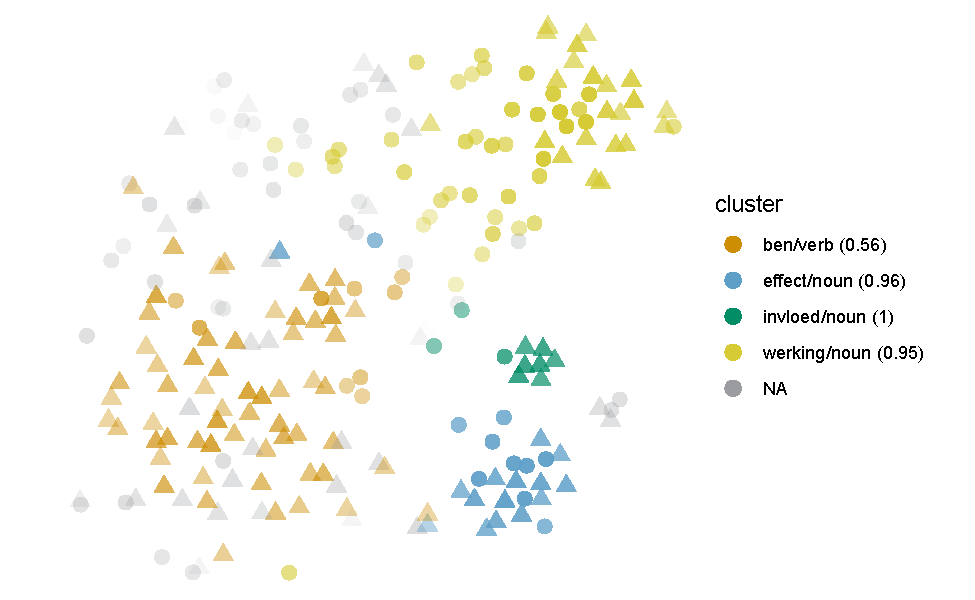
\includegraphics{phdThesis_files/figure-latex/heilzaam-1.pdf}
\caption{\label{fig:heilzaam}Cloud of \emph{heilzaam}: heilzaam.BOWbound10all.PPMIweight.LENGTHFOC.SOCPOSall.}
\end{figure}

This is an issue if we come to the modelling expecting lexical collocates, such as \emph{werking} `werking', \emph{effect}, and \emph{invloed} `influence', to unequivocally represent different dictionary senses. On the other hand, \emph{ben} `to be' and \emph{werk} `to work, to have an effect' (of which \emph{werking} is a nominalisation), co-occur with the tokens in the orange cluster, dominated by the general sense, and less so outside this cluster; see examples (9) and (10).
In other words, the most frequent nouns modified by \emph{heilzaam} `beneficial' tend to occur in attributive constructions (particularly \emph{een heilzame werking hebben} `to have a beneficial/healing effect/power' and \emph{de heilzame werking van} `the beneficial/healing effect/power of') and for either sense, whereas the predicative constructions present a wider variety of nouns and a stronger tendency towards the general sense.

\begin{enumerate}
\def\labelenumi{(\arabic{enumi})}
\setcounter{enumi}{8}
\item
  ten goede komen . Versterking \emph{van} \emph{de} politieke controle \emph{op} \emph{de} \emph{Commissie} \emph{kan} \textbf{heilzaam} \emph{zijn} \emph{maar} \emph{de} \emph{huidige} ongenuanceerde \emph{discussie} \emph{is} \emph{gevaarlijk} \emph{voor} Europees beleid en besluitvorming . (\emph{NA}, 1999-03-18, Art. 45)
\item
  In een vervolg op een project met Ensemble Loos onderzoekt het gezelschap in Blood on the floor wederom of de samenwerking tussen frank en vrij improviserende jazzmuzikanten enerzijds en dapper maten tellende en genoteerde \emph{noten} \emph{spelende} \emph{musici} \emph{anderzijds} \textbf{heilzaam} \emph{kan} \emph{werken} . Turnage heeft de zaak naar eigen zeggen niet op de (\emph{Het Parool}, 1999-03-23, Art. 79)
\end{enumerate}

\hypertarget{perfect-clouds}{%
\subsection{Perfect clouds}\label{perfect-clouds}}

In a few cases we can see clusters characterized by one dominant context word that perfectly match a sense, or at least its clustered tokens. These are normally fixed expressions, at least to a degree: the definition itself may require a specific expression, such as \emph{representatieve staal} `representative sample'.

An interesting example is shown in Figure \ref{fig:schaal}, a model of the noun \emph{schaal} `scale, dish'. In the plot, the `scale' homonym is represented by circles (`a range of values, e.g.~the scale of Richter, a scale from 1 to 5'), squares (`magnitude, e.g.~on a large scale') and a few triangles (`ratio, e.g.~a scale of 1:20'), whereas the `dish' homonym is represented by crosses (`shallow wide dish') and crossed squares (`dish of a scale').
Both the `range' and the `dish of scale' senses, exemplified in (11) and (12), have a perfect match (or almost) with an HDBSCAN cluster, represented by a context word with perfect F-score. All the \emph{schaal} tokens co-occurring with \emph{Richter} are grouped in the red cluster, and cover almost the full range of attestations of the `range' sense, and all the tokens co-occurring with \emph{gewicht} `weight' are grouped in the light blue cluster and cover all the attestations of a `dish of a scale' sense.

\begin{enumerate}
\def\labelenumi{(\arabic{enumi})}
\setcounter{enumi}{10}
\item
  Wenen , Beneden-Oostenrijk en Burgenland zijn dinsdagochtend opgeschrikt door een \emph{aardschok} \emph{van} \emph{4,8} \emph{op} \emph{de} \textbf{schaal} \emph{van} \emph{Richter} . \emph{De} \emph{bevolking} van de hoofdstad werd daardoor bij het krieken (\emph{NA}, 2000-07-12, Art. 4)
\item
  Daarom is het van belang dat Nederland zich deze week achter de VS heeft geschaard , ook al legt ons land natuurlijk minder \emph{gewicht} \emph{in} \emph{de} \textbf{schaal} dan \emph{Duitsland} \emph{in} het \emph{Europese} debat over de al dan niet noodzakelijke toestemming van de Veiligheidsraad voor militaire actie tegen Irak . (\emph{NRC Handelsblad}, 2002-09-07, Art. 160)
\end{enumerate}

In a way, the phenomenon indicates a fixed, idiomatic expression: a combination of two or more words that fully represents a sense. However, the picture is more nuanced.
First, technically, the `range' sense can potentially occur with more context words than \emph{Richter}. In fact, one of the examples given to the annotators is \emph{schaal van Celsius} `Celsius scale', as well a pattern like the one found in (13), one of the orange circles at the top of Figure \ref{fig:schaal}. However, in the corpus used for these studies, \emph{Celsius} does not co-occur with \emph{schaal} in a symmetric window of 4; moreover, of the 32 tokens of this sense attested in this model, 22 co-occur with \emph{Richter}, 3 match with the pattern from (13), and the rest exhibit less fixed patterns or the infrequent \emph{glijdende schaal} `slippery slope' construction. The few matching (13) are more readily clustered with other tokens co-occurring with the preposition \emph{op}, such as (14). In other words, in the register of newspapers, the `range' sense of \emph{schaal} is almost completely exhausted in the \emph{schaal van Richter} `Richter scale' expression.

\begin{enumerate}
\def\labelenumi{(\arabic{enumi})}
\setcounter{enumi}{12}
\item
  " Misschien deelt de computer mij op grond \emph{van} \emph{statistische} analyses \emph{op} \emph{een} \textbf{schaal} \emph{van} \emph{1} \emph{tot} \emph{12} \emph{in} categorie 3 ' , zegt woordvoerder B. Crouwers van de registratiekamer . (\emph{NRC Handelsblad}, 1999-01-09, Art. 10)
\item
  . Die stad vormde de opmaat tot de latere \emph{collectieve} \emph{regelingen} \emph{op} \emph{nationale} \textbf{schaal} , stellen \emph{de} auteurs , in navolging van socioloog prof. dr. Abram de Swaan . (\emph{Volkskrant}, 2003-05-03, Art. 253)
\end{enumerate}

Second, the `dish of a scale' sense need to be used in the metaphorical expression illustrated in (12), but that is indeed the case in our data. Next to \emph{gewicht} `weight', these tokens also mostly co-occur with \emph{leg} `to lie, to place' or, in lesser degree, with \emph{werpen} `to throw'. Even in other models, this cluster tends to be built around the co-occurrence with \emph{gewicht} `weight', normally excluding tokens that only co-occur with \emph{leg} `to lie, to place', which do not belong to the same sense any more.



\begin{figure}
\centering
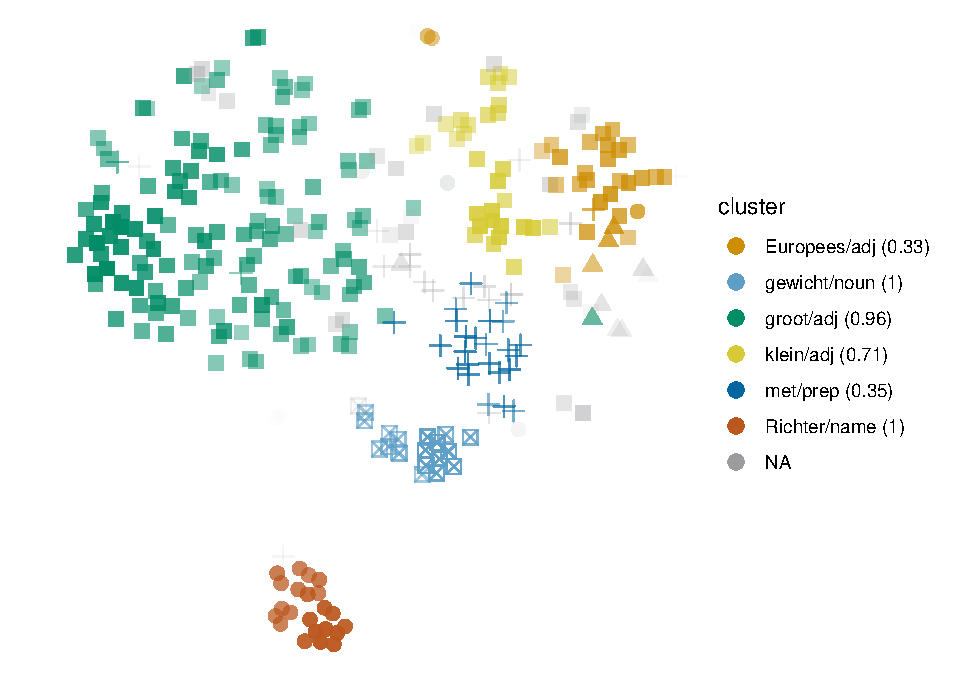
\includegraphics{phdThesis_files/figure-latex/schaal-1.pdf}
\caption{\label{fig:schaal}Cloud of \emph{schaal}: schaal.BOWnobound5all.PPMIweight.LENGTHFOC.SOCPOSall.}
\end{figure}

These examples don't disprove the possibility of clouds dominated by a collocate perfectly covering a sense, as long as we keep in mind the characteristics and limitations of the corpus we are studying and the difference between describing ``how a sense is used'' and "how a sense is used \emph{in this particular corpus}.

\hypertarget{prototypical-context}{%
\subsection{(Proto)typical context}\label{prototypical-context}}

The most frequent phenomenon --- especially among Cumulus clouds --- is a cluster dominated by one context word or group of co-occurring context words that represents a (proto)typical context of a sense. It may be \emph{the} prototypical context, if the rest of the the sense is discarded as noise or spread around less clear clusters, but we might also find multiple clusters representing different typical contexts of the same sense. Neither t-SNE nor HDBSCAN can tell whether one of these contexts is more central than the other, at least not in the same sense we would expect from prototype theory. Denser areas of tokens, as perceived by HDBSCAN, are those where many tokens are very similar to each other. The more tokens are similar, and the more similar they are, the denser the area. As we will see in this example, this is not a good proxy for prototypicality.

One of the most clear examples of this phenomenon is found in \emph{heffen} `to levy/to lift', whose typical objects are also characteristic of its two main senses (see Figure \ref{fig:heffen}). On the one hand, the `to levy' sense occurs mostly with \emph{belasting} `tax', \emph{tol} `toll'{[}\^{}Typical of the Netherlandic sources, since tolls are not levied in Flanders.{]}, and \emph{accijns} `excise', as shown in (15) through (17). Their frequencies are large enough to form three distinct clusters, which tend to merge in the following levels of the HDBSCAN hierarchy, that is, they are closer to each other than to the clusters of the other sense. On the other hand, the `to lift' sense occurs with \emph{glas} `glass', where the final expression \emph{een glas(je) heffen op} takes a metonymical meaning `to give a toast to' (see (18)), and with the body-parts \emph{hand}, \emph{arm} and \emph{vinger} `finger', in which they might take other metonymical meanings. The latter group does not really belong to this ``collocation'' category but to ``semantic preference'' (see Section @(semantic-preference)).

\begin{enumerate}
\def\labelenumi{(\arabic{enumi})}
\setcounter{enumi}{14}
\item
  Op het inkomen boven \emph{die} drie miljoen \emph{gulden} \emph{wil} De \emph{Waal} \emph{honderd} \emph{procent} \emph{belasting} \textbf{heffen} . De opbrengst gaat naar de allerarmsten . Ah , een (\emph{Het Parool}, 2001-05-02, Art. 99)
\item
  Mobiliteitsproblemen , rekeningrijden , op een andere manier het \emph{gebruik} van de \emph{weg} \emph{belasten} , kilometers \emph{tellen} , \emph{tol} \textbf{heffen} - de \emph{mogelijkheden} \emph{om} de ingebouwde chip \emph{te} benutten zijn vrijwel onbeperkt . (\emph{NRC Handelsblad}, 1999-10-02, Art. 31)
\item
  De accijnsheffingen tussen de verschillende landen variëren zeer sterk ten opzichte van elkaar , waardoor er aan weerszijden van het door Bolkestein voorgestelde minimum een discrepantie komt : in landen als Groot-Brittannië ( waar de accijnzen op 742 euro per 1.000 liter liggen ) , Italië \emph{en} \emph{Duitsland} ( \emph{die} \emph{beide} \emph{accijnzen} \emph{boven} de \emph{400} \emph{euro} \textbf{heffen} ) komt de \emph{harmonisering} ten goede van de transportsector , terwijl in andere landen ( zoals Spanje , Ierland , Oostenrijk , Finland en België , waar de accijnzen rond de 300 euro schommelen ) de overheid een voordeel heeft . (\emph{NA}, 2002-07-25, Art. 104)
\item
  met het vertrouwde pintje . Nog \emph{twaalf} andere deelnemers \emph{konden} \emph{maandagavond} \emph{het} \emph{glas} \textbf{heffen} \emph{op} de \emph{hoogste} \emph{winst} . De dertien deelnemers die 5-9-15-23-29-32 hadden aangekruist , (\emph{NA}, 2004-10-20, Art. 150)
\end{enumerate}

As we can see in Figure \ref{fig:heffen}, the model is very successful at separating the two senses, and the clusters are semantically homogeneous: the most relevant collocates of \emph{heffen} `to levy/to lift' are distinctive of one or the other of its senses. Crucially, no single cluster is even close to covering a full sense; instead, each of them represents a prototypical pattern that stands out due to its frequency, internal coherence and distinctiveness.
It seems reasonable to map the clusters to prototypical patterns because of their frequency and distinctiveness, but we should be careful about how we apply the results of the modelling to this kind of semantic analysis. From the perspective of prototype theory, a feature of a category is more central if it is more frequent, i.e.~it is shared by more members, while a member is more central if it exhibits more of the defining features of the categories. As such, within the `to levy' sense, the \emph{belasting heffen} `to levy taxes' pattern is the most central, and tokens instantiating such a pattern will be more central. In contrast, HDBSCAN prioritises dense areas, that is, groups of tokens that are very similar to each other. Thus, membership probabilities, which we might be tempted to use as proxy for centrality, indicate internal consistency, lack of variation. From such a perspective, given that \emph{belasting heffen} `to levy taxes' is more frequent and applies to a wider variety of contexts than the other two patterns of `to levy', its area is less dense, and its tokens have lower membership probabilities within a compound `to levy' clusters.

In other words, the models can offer us typical patterns of a lemma and of its senses and tell us how distinctive they are from each other and how much internal variation they present. Beyond this information, they don't map in a straightforward manner to our understanding of prototypicality.



\begin{figure}
\centering
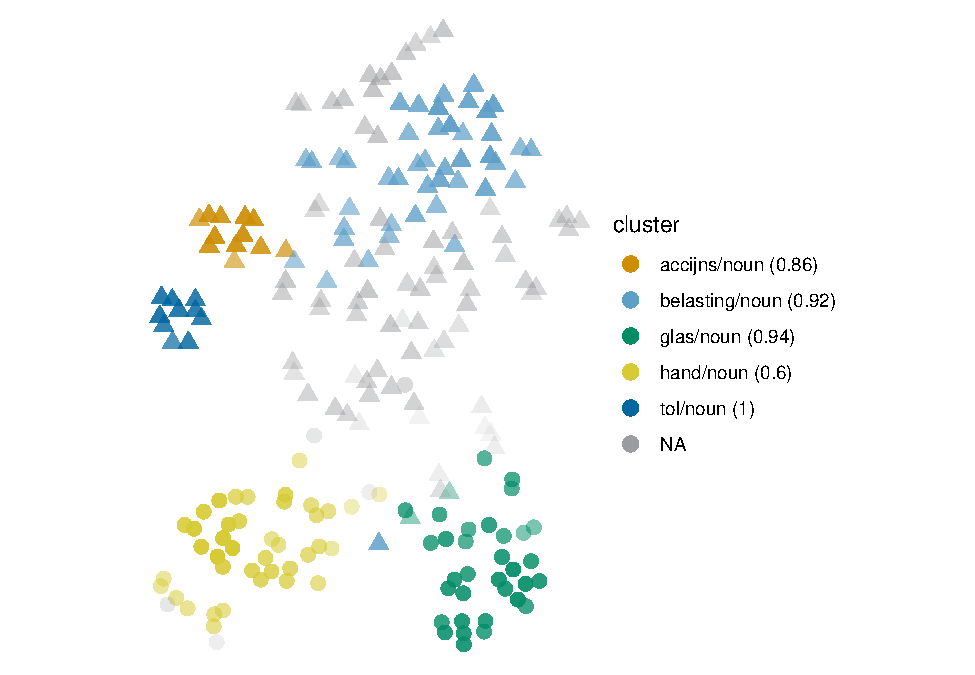
\includegraphics{phdThesis_files/figure-latex/heffen-1.pdf}
\caption{\label{fig:heffen}Cloud of \emph{heffen}: heffen.BOWbound10all.PPMIweight.LENGTHFOC.SOCPOSnav.}
\end{figure}

It must be noted that clusters defined by collocations may not be just characterized by one single context word, but by multiple partially co-occurring context words. A clear example is \emph{hachelijk} `dangerous' (Figure \ref{fig:hachelijk}), where both senses are characterized by prototypical contexts, exemplified in (19) through (24): \emph{onderneming} `undertaking', \emph{zaak} `business' and \emph{avontuur} `adventure' for the `potentially dangerous' sense, \emph{moment}, \emph{situatie} `situation', and \emph{positie} `position' for the `critical' sense.
These six frequent context words are paradigmatic alternatives of each other, all taking the slot of the modified noun, the entity characterized as dangerous or critical. However, unlike its very type-level near neighbour \emph{situatie} `situation', \emph{positie} `position' may also co-occur with \emph{bevrijd} `to free' (and \emph{uit} `from') and, additionally, with \emph{brandweer} `firefighter', typically in Belgian contexts. The frequency of these co-occurrences in the sample, next to the type-level dissimilarity between these three lexical items, splits the co-occurrences with \emph{positie} `position' in three clusters (in light blue, green and red in Figure \ref{fig:hachelijk}), based on these combinations.

\begin{enumerate}
\def\labelenumi{(\arabic{enumi})}
\setcounter{enumi}{18}
\item
  Het is geen gewaagde stelling dat de deelname van de LPF aan de \emph{regering} \emph{een} \textbf{hachelijke} \emph{onderneming} \emph{blijft} . De situatie waarin de LPF is terechtgekomen , is het (\emph{Volkskrant}, 2002-08-05, Art. 46)
\item
  Daar baseerden de media zich op slechts één bron , en elke journalist weet dat \emph{dat} \emph{een} \textbf{hachelijke} \emph{zaak} \emph{is} . ' Jacques Wallage , burgemeester van Groningen : ' Vroeger (\emph{Volkskrant}, 2004-05-05, Art. 42)
\item
  Het stadsautootje voelt zich beter thuis op het gladde asfaltlint van de snelweg en zolang er geen fikse zijwind staat - want hij is daar door z'n relatief hoge bouw én achterwielaandrijving erg gevoelig voor , met storm opzij is het \emph{inhalen} van \emph{een} \emph{vrachtwagen} \emph{een} \textbf{hachelijk} \emph{avontuur} - \emph{kan} je daar heel relaxed grote afstanden mee afleggen . Je (\emph{Het Parool}, 2000-03-17, Art. 34)
\item
  de reguliere competitie viel er toch iets te beleven . \emph{Kortrijk} \emph{beleefde} \emph{enkele} \textbf{hachelijke} \emph{momenten} tegen \emph{Brussels} , dat in zijn ondiep bad bewees zijn vierde plaats in de play-offs waard te zijn . (\emph{NA}, 2001-05-14, Art. 375)
\item
  als interne Palestijnse factoren . Kort maar krachtig staat er : " De \textbf{hachelijke} \emph{situatie} van \emph{Palestina} \emph{is} vooral een interne aangelegenheid , hoewel de bezetting en de confrontatie met Israël er de context voor schept . (\emph{NA}, 2004-10-02, Art. 162)
\item
  Nederlandse Wendelien van Oldenborgh . Zij toont knappe filmpjes , \emph{opgenomen} \emph{vanuit} de \textbf{hachelijke} \emph{positie} van \emph{een} deltavlieger , ze doorkruist de ruimte met een betreedbare loopbrug om ten slotte met haar ' pin drawings ' een wervelend veld van spelden te prikken op een piepschuimen plattegrond van de exporuimte in de centrale bib . (\emph{NA}, 1999-06-07, Art. 126)
\end{enumerate}

It would be hard to argue about the relative centrality of the three \emph{positie} clusters. They result from the combination of three features, and each cluster exhibits a different degree of membership based on how many of these overlapping features it co-occurs with. At the same time, they have a distinctive regional distribution. Based on this data, we might said that a prototypical context of \emph{hachelijke posities} `dangerous/critical positions' in Flanders is a situation in which firefighters free someone/something from them, while this core is not present, or at least not nearly as relevant, in the Netherlandic data. We might also say that the same situation is not typical of \emph{hachelijke situaties} `dangerous/critical situations', and this therefore presents a (local) distributional difference between two types that otherwise, at corpus level, are near neighbours.



\begin{figure}
\centering
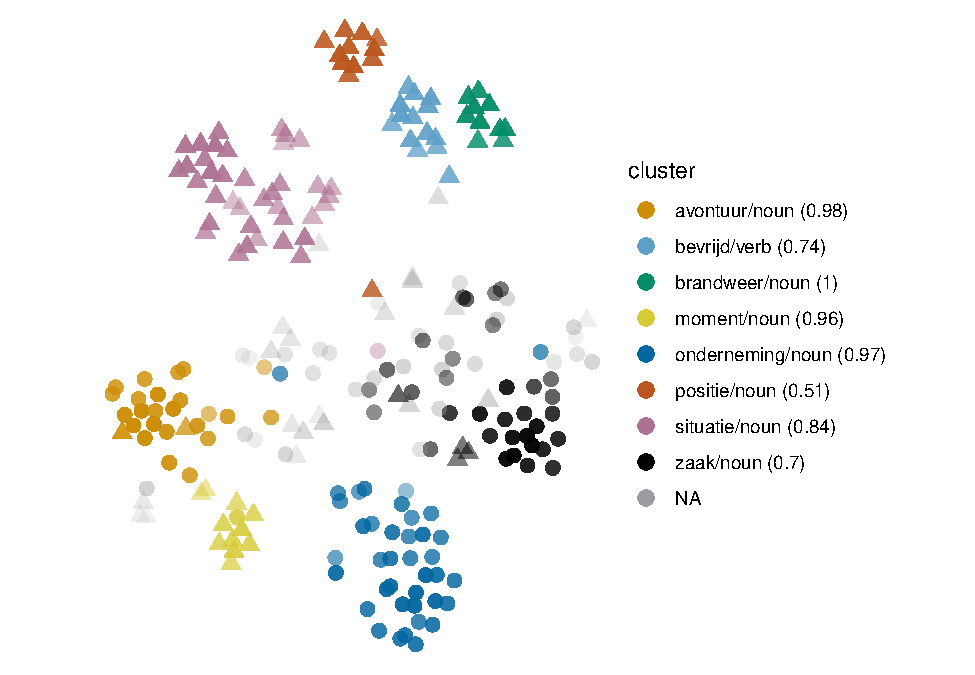
\includegraphics{phdThesis_files/figure-latex/hachelijk-1.pdf}
\caption{\label{fig:hachelijk}Cloud of \emph{hachelijk}: hachelijk.BOWbound5all.PPMIweight.LENGTHFOC.SOCPOSall.}
\end{figure}

\hypertarget{profiling}{%
\subsection{Profiling}\label{profiling}}

Clusters dominated by a context word may not only represent a typical context within a sense, but also one that highlights a different dimension of such sense than other clusters. This is not extremely frequent and requires an extra layer of interpretation, but it is an additional explanation to some of the clustering solutions.

One example is given by the `substance' meaning of \emph{stof}.
Within this sense, we tend to find clusters dominated by \emph{gevaarlijk} `dangerous', \emph{schadelijk} `harmful' (which also attracts \emph{kankerwekkend} `carcinogenic') and \emph{giftig} `poisonous' (which often attracts \emph{chemisch} `chemical'). These dominant context words are nearest neighbours at type-level, and the clusters they govern belong to the same branch in the HDBSCAN hierarchy.

However, we can find additional information, among the context words that co-occur with them, which suggests that frequency is not the only responsible for their separated clusters. Concretely, the tokens in the cluster dominated by \emph{schadelijk} `harmful' tend to focus on the environment and composition of substances, as indicated by the co-occurrence with \emph{uitstoot} `emissions', \emph{lucht} `air', \emph{stank} `stench' and \emph{bevat} `to contain'; meanwhile, those in the cluster dominated by \emph{giftig} `poisonous' focus on the context of drugs or profile the liberation of substances, with context words such as \emph{vorm} `to form', \emph{kom\_vrij} `to be released' and \emph{drugsbebruik} `drug use'.
This effect of the less frequent context words is one of the consequences of less restrictive models: at some levels of analysis, one word (\emph{gevaarlijk} `dangerous', \emph{schadelijk} `harmful'\ldots) might be enough to disambiguate the target, but this extra information enriches our understanding of how the words are actually used. It is also contextualized information: not just about how \emph{stof} `substance' is used and what it means, but how it is used (and what it means) when in combination with certain frequent collocates.

\hypertarget{colligation}{%
\section{Lexically instantiated colligation}\label{colligation}}

Some defined by the presence of a word that indicates a grammatical preference or tendency (valency?), such as passive constructions.

\hypertarget{heterogeneous}{%
\subsection{Heterogeneous}\label{heterogeneous}}

The senses of \emph{herstructureren} emerge from a combination of specialization (whether it's specifically applied to companies) and argument structure (intransitive or transitive constructions). The most frequent lexical collocates, \emph{bedrijf} and \emph{grondig}, rarely co-occur with each other or with \emph{worden}, which indicates passive construction and therefore a transitive form. The clusters in various models tend to be built around these three context words, grouping most of the transitive uses, either company-specific or not, in the \emph{worden} clusters, such as the blue one in Figure \ref{fig:herstructureren}.



\begin{figure}
\centering
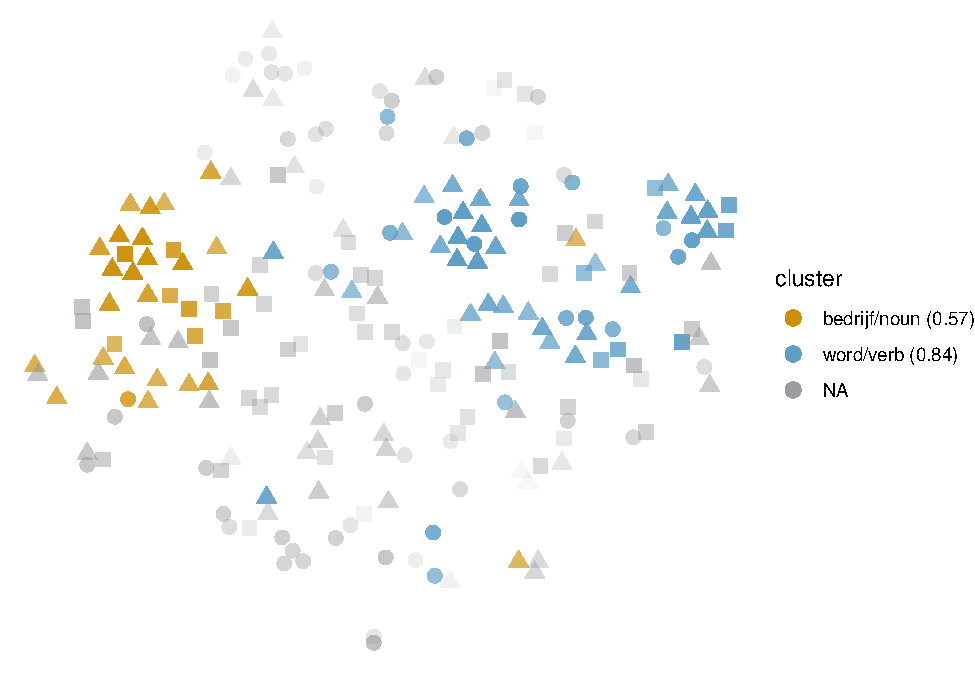
\includegraphics{phdThesis_files/figure-latex/herstructureren-1.pdf}
\caption{\label{fig:herstructureren}Cloud of \emph{herstructureren}.}
\end{figure}

\hypertarget{one-sense}{%
\subsection{One sense}\label{one-sense}}

While a rare thing, we might be able to pinpoint a specific sense based on a collocation that points to a grammatical pattern. One clear case is the reflexive sense of \emph{herhalen}, characterized by its co-occurrence with \emph{zich} (Figure \ref{fig:herhalen}), which is not captured by \texttt{FOC-POS:lex} models. Even when it is, it might further be split by the co-occurrence with \emph{geschiedenis} in about half the attestations.

We expected this result in other lemmas with purely reflexive senses as well, but it is not easy to achieve. For example, \emph{herinneren} is often split in three major clusters with a small one for \emph{eraan} that is sometimes absorbed by a larger cloud. The large ones are characterized by \emph{aan}, \emph{ik} and \emph{me}, and \emph{zich}, respectively. Both the first and third person are frequent enough within the reflexive sense to give rise to their own clusters. In the case of \emph{diskwalificeren}, instead, the reflexive sense is typically (but not always) absorbed within the transitive sense that matches it semantically, i.e.~the non sports-related sense.



\begin{figure}
\centering
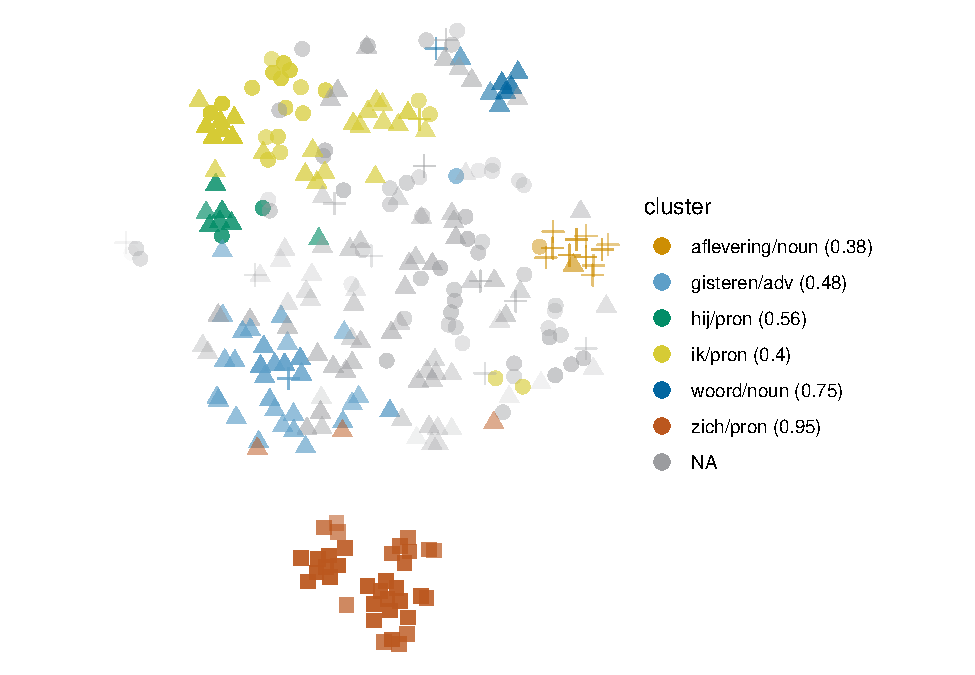
\includegraphics{phdThesis_files/figure-latex/herhalen-1.pdf}
\caption{\label{fig:herhalen}Cloud of \emph{herhalen}.}
\end{figure}

\hypertarget{prototypical-context-1}{%
\subsection{(Proto)typical context}\label{prototypical-context-1}}

The most clear example of clusters indicating typical contexts of a sense and defined by grammatical collocates is given by \emph{diskwalificeren} and the tendency of the sports-specific sense to co-occur with \emph{worden}. This is shown by the yellow cluster in Figure \ref{fig:diskwalificeren}.



\begin{figure}
\centering
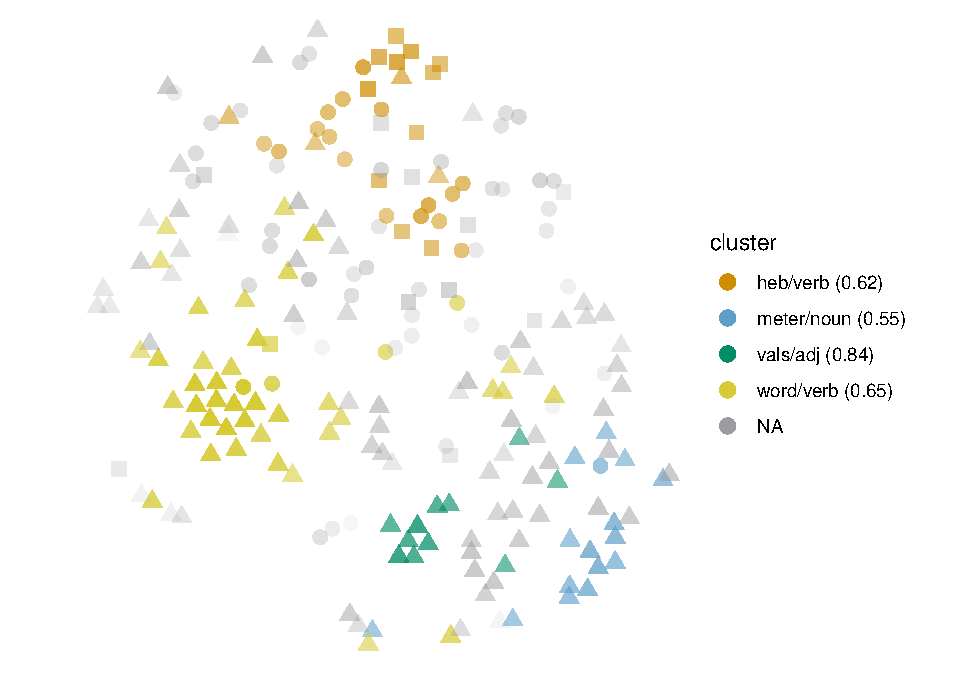
\includegraphics{phdThesis_files/figure-latex/diskwalificeren-1.pdf}
\caption{\label{fig:diskwalificeren}Cloud of \emph{diskwalificeren}.}
\end{figure}

\hypertarget{profiling-1}{%
\subsection{Profiling}\label{profiling-1}}

The `horde' sense of \emph{horde} tends to co-occur with \emph{tourist} and \emph{journalist} in this corpus. The two collocates are quite similar to each other, but the rest of the context words in their clusters point towards a different dimension of the `horde' sense: hordes of journalists/photographers will surround and follow celebrities (\emph{omringen}, \emph{opwachten}, \emph{achtervolgen}), while hordes of tourists will instead flood and move around in the city (\emph{toestromen}, \emph{stad}). This is strengthened by the co-occurrence of the preposition \emph{door} and the verb \emph{worden} with \emph{journalist} --- to the point that the corresponding cluster is better represented by \emph{door} than by \emph{journalist} in Figure \ref{fig:horde} ---, while \emph{toerist} prefers \emph{naar}.



\begin{figure}
\centering
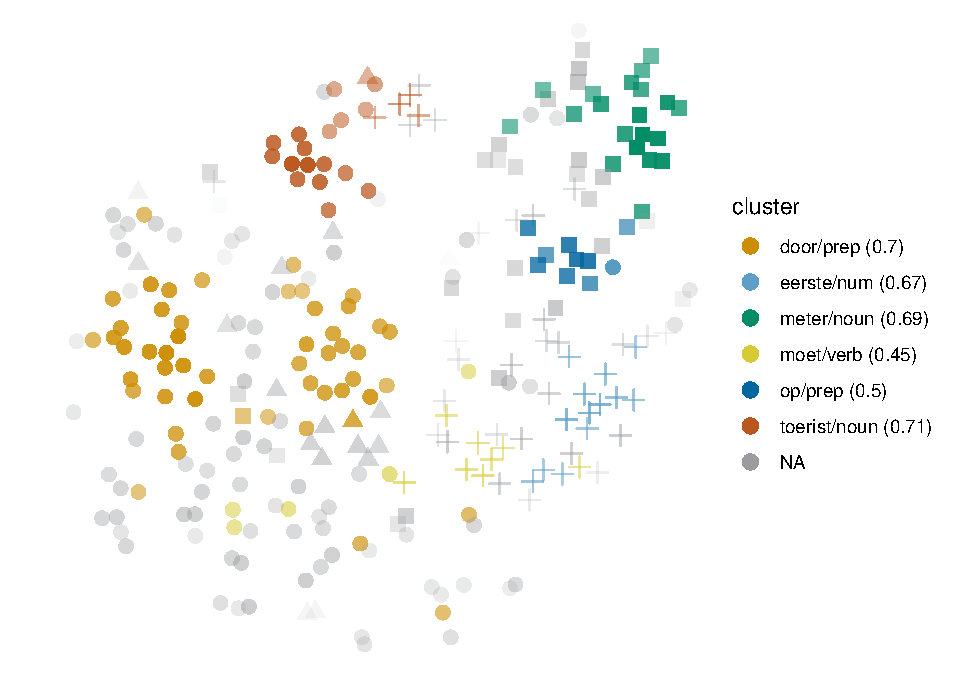
\includegraphics{phdThesis_files/figure-latex/horde-1.pdf}
\caption{\label{fig:horde}Cloud of \emph{horde}.}
\end{figure}

\hypertarget{semantic-preference}{%
\section{Semantic preference}\label{semantic-preference}}

Clusters defined by multiple infrequent similar context words.

\hypertarget{heterogeneous-1}{%
\subsection{Heterogeneous}\label{heterogeneous-1}}

Just like we can have clusters dominated by one context word that is not characteristic of one sense, we can have clusters dominated by multiple similar context words that are not characteristic of any sense. This is the case of names of colours and clothes, which (somehow) includes \emph{haar} `hair'. As a result, \emph{grijs} tokens pointing to the general grey things and to, specifically, grey/white hairs, are clustered together (the large light blue cluster in Figure \ref{fig:grijs}). Note that, visually, the two senses occupy opposite halves of this cluster.

A similar group of context words is responsible for joining the `fabric' and `lit. dust' senses of \emph{stof}, even across homonyms.



\begin{figure}
\centering
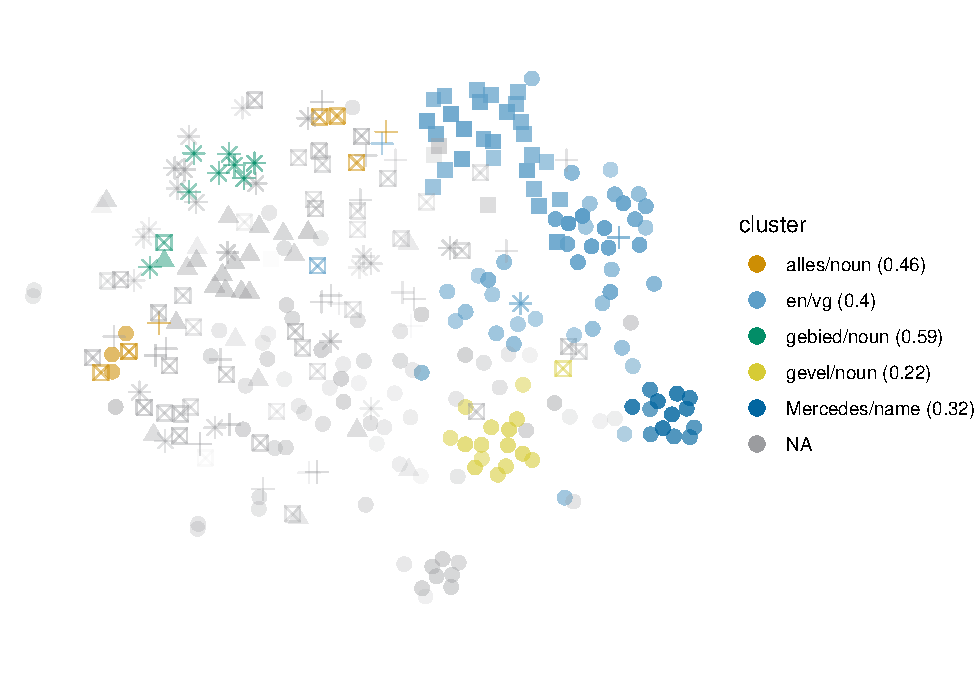
\includegraphics{phdThesis_files/figure-latex/grijs-1.pdf}
\caption{\label{fig:grijs}Cloud of \emph{grijs}.}
\end{figure}

Another case is the set of juridical terms in \emph{herroepen}: the most frequent of them, \emph{uitspraak}, is ambiguous: when it means `statement', \emph{herroepen} means `to retract', whereas its `verdict' sense invokes the `to annul' sense of \emph{herroepen}. Both situations occur in the sample, but the most frequent one is the `statement' sense, that is, not the one of the juridical field. In some models, the \emph{uitspraak} tokens form their own cluster, next to another cluster with context words such as \emph{rechtbank}, \emph{vonnis}, etc., in which case the former is heterogeneous and the latter, homogeneous. In other models (see Figure \ref{fig:herroepen}), both groups are clustered together, leading to a heterogeneous cluster brought together by semantic preference, although again, visually they are distinguishable. At the same time, \emph{verklaring} and \emph{bekentenis} also could be considered part of the same semantic field, in broad terms, but they point to a different aspect, i.e.~a different frame within the same field of legal action, and, correspondingly, their type-level vectors are different and they tend to represent distinct, homogeneous clusters.



\begin{figure}
\centering
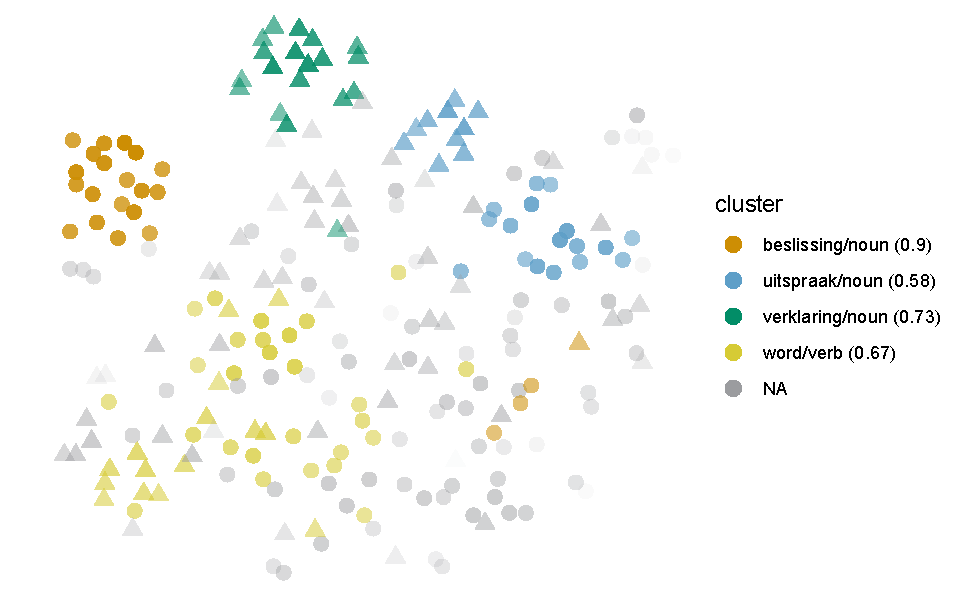
\includegraphics{phdThesis_files/figure-latex/herroepen-1.pdf}
\caption{\label{fig:herroepen}Cloud of \emph{herroepen}.}
\end{figure}

\hypertarget{one-sense-1}{%
\subsection{One sense}\label{one-sense-1}}

A few senses can be completely clustered by groups of similar context words, as long as we don't mind too much the portion of the sense that was excluded as noise. One of these cases is the same group of \emph{schaal} tokens represented by \emph{Richter}, which, in models that exclude \emph{Richter}, can be grouped by \emph{kracht}, \emph{aardbeving} and related context words. Another example is found in \emph{haken}, where the `make someone trip' sense is characterized by football-related terms (\emph{strafschop(sgebied)}, \emph{penalty}, \emph{scheidsrechter}\ldots), and the very infrequent `crochet' sense, by \emph{breien}, \emph{naaien}, \emph{hobby} and similar. They are represented in the dark blue and light blue clusters in Figure \ref{fig:haken} respectively.



\begin{figure}
\centering
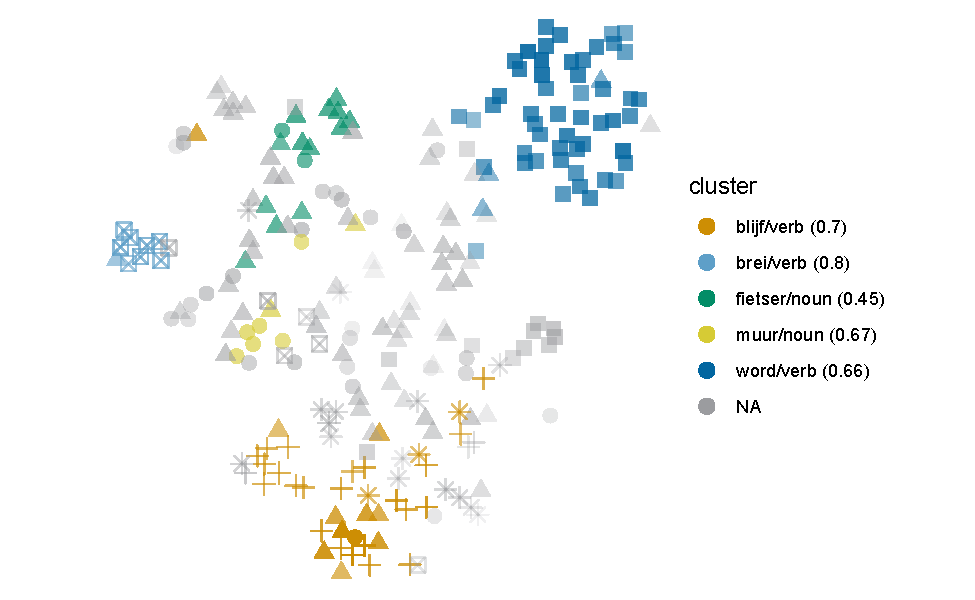
\includegraphics{phdThesis_files/figure-latex/haken-1.pdf}
\caption{\label{fig:haken}Cloud of \emph{haken}.}
\end{figure}

\hypertarget{prototypical-context-2}{%
\subsection{(Proto)typical context}\label{prototypical-context-2}}

There are several examples of clusters defined by semantically similar infrequent context words, representing typical contexts of a sense. In Figure \ref{fig:grijs}, for example, the dark blue cluster is represented by cars, mostly thanks to \emph{Mercedes} and \emph{Opel}, but also other brands. In the case of some lemmas, particularly \emph{dof}, some models split the tokens co-occurring with different related context words in multiple clusters (\emph{klinken}, \emph{knal}, \emph{klap}, \emph{dreun}) while others group them together in one large cluster defined by a semantic preference indicative of a sense (in this case, `dull (sound)').

A typical semantic group is the culinary one: found with \emph{schaal} `dish' and with \emph{heet} (the red cluster in Figure \ref{fig:heet}). In the case of \emph{heet}, almost all the tokens co-occurring in this cluster refer to literally hot foods and drinks, although the full expression might be idiomatic, i.e.~\emph{de soep niet zo heet eten}, and only a few of them belong to the much less frequent sense `spicy'. In other models, either the \emph{soep + eten} tokens or the \emph{water} tokens might form separate clusters. In addition, \emph{aardappel} is very similar to the other context words in this group at the type-level, but it still tends to form its own cluster, thanks to both its frequency and the distinctiveness of its larger cotext.



\begin{figure}
\centering
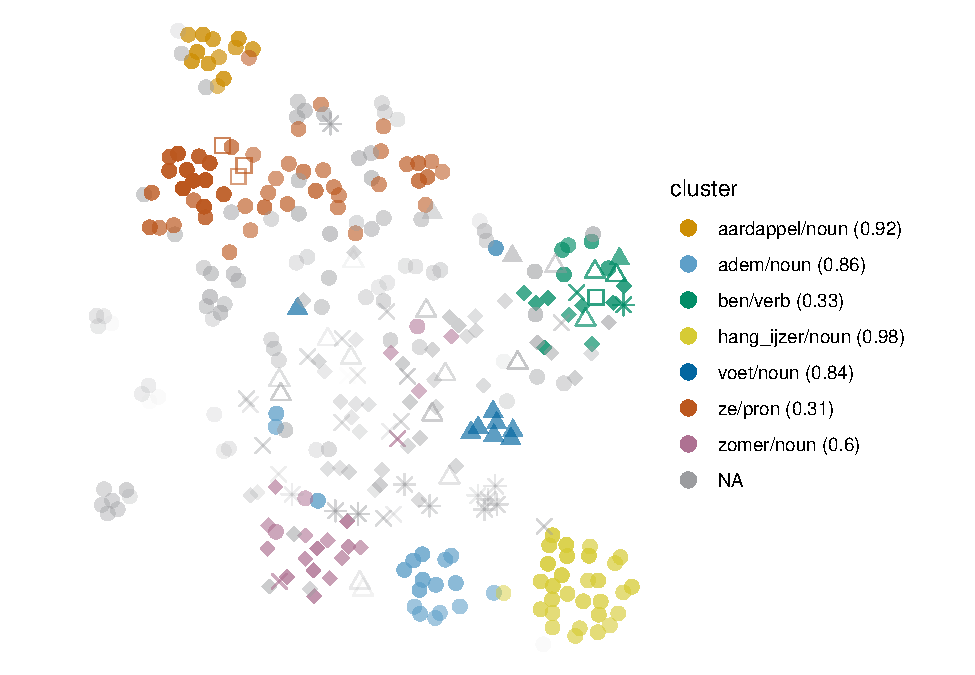
\includegraphics{phdThesis_files/figure-latex/heet-1.pdf}
\caption{\label{fig:heet}Cloud of \emph{heet}.}
\end{figure}

\hypertarget{profiling-2}{%
\subsection{Profiling}\label{profiling-2}}

Among the senses of \emph{geldig}, the specific one related to regulated validity is much more frequent than the general one. In addition, models tend to distinguish two dimensions of this regulated validity, either as clusters characterized by semantic preference, or simply as regions in the t-SNE plot. One of the groups represents contexts in which someone has to present (\emph{voorleggen}, \emph{bezitten}\ldots) some form of identification (\emph{rijbewijs}, \emph{paspoort}, etc.), while the other represents other kinds of documents (\emph{ticket}, \emph{abonnement}) in which the duration of its validity is more salient (\emph{tot}, \emph{maand}, numbers\ldots). While it is not clear from their most representative context words, these groups are illustrated as the green and yellow clusters, respectively, in Figure \ref{fig:geldig}.



\begin{figure}
\centering
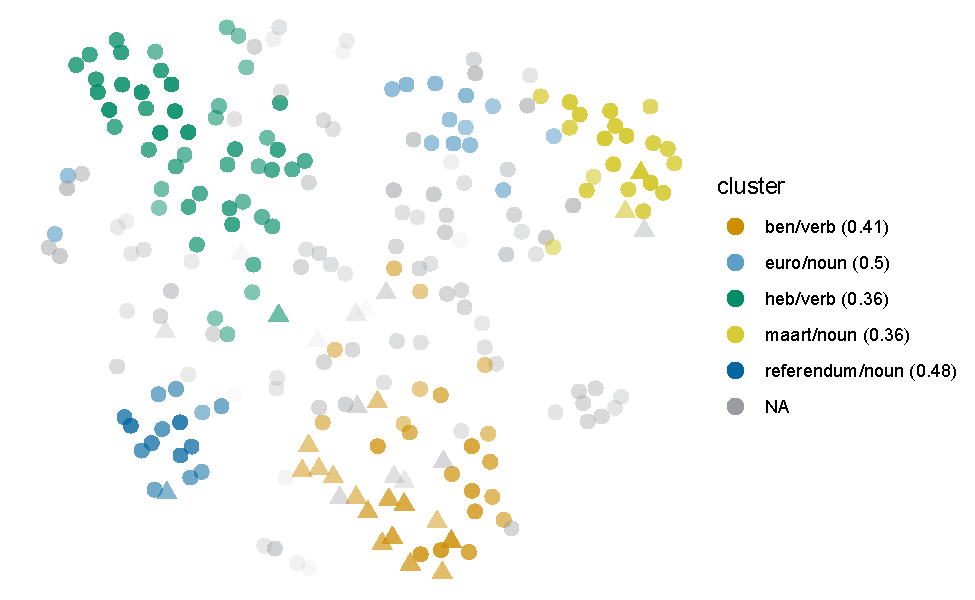
\includegraphics{phdThesis_files/figure-latex/geldig-1.pdf}
\caption{\label{fig:geldig}Cloud of \emph{geldig}.}
\end{figure}

\hypertarget{openchoice}{%
\section{Near-open choice}\label{openchoice}}

Most Cirrus clouds, as well as the Cumulonimbus, are not really grouped by one dominant context word or by a set of similar words. It is not clear what brings the tokens together. Naturally, this mostly leads to heterogeneous clouds, but occasionally we might find more homogeneous ones among them. The principle behind this category is not so much that the clusters are bad, but that the lemmas seem to follow more of an open-choice principle: a wider variety of options, so that the most powerful collocates barely group a couple of tokens. By definition they aren't patterns, so they cannot represent prototypical contexts of a sense, but some of these clusters do happen to be quite homogeneous.

\hypertarget{heterogeneous-2}{%
\subsection{Heterogeneous}\label{heterogeneous-2}}

The most common situation in clusters that are not explained by a dominant context word or semantic preference, especially when they are Cumulonimbus, is that they are semantically heterogeneous. One such example is the Cumulonimbus (the large cloud) of \emph{helpen} in Figure \ref{fig:helpen}, formed in opposition to the smaller Stratocumulus, which is also an heterogeneous cloud formed by semantic preference for kinship terms.



\begin{figure}
\centering
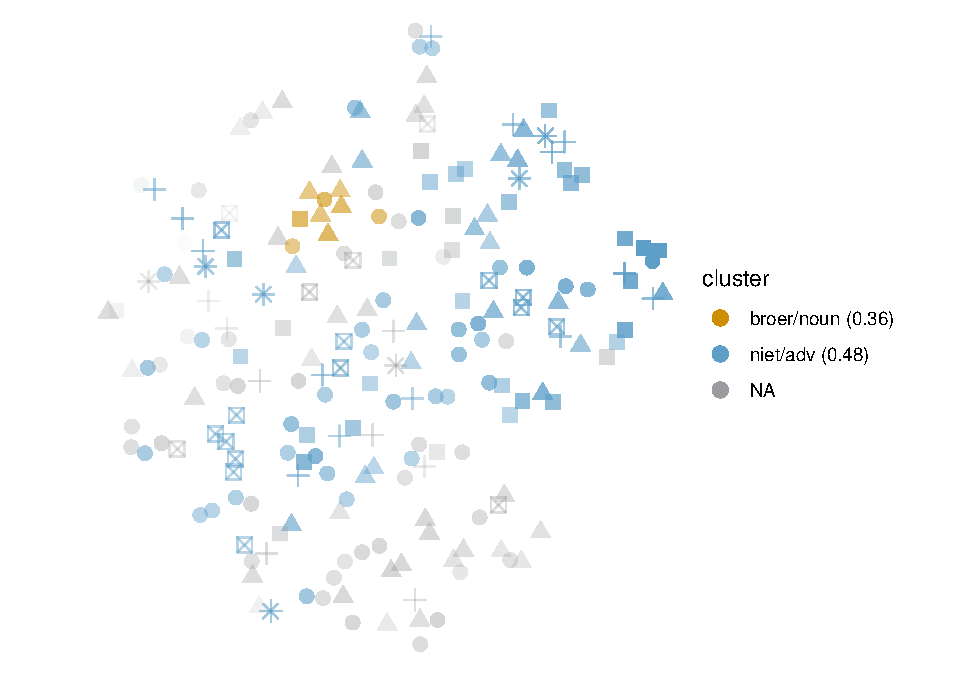
\includegraphics{phdThesis_files/figure-latex/helpen-1.pdf}
\caption{\label{fig:helpen}Cloud of \emph{helpen}.}
\end{figure}

\hypertarget{one-sense-2}{%
\subsection{One sense}\label{one-sense-2}}

Cumulonimbus clouds are a sort of bag with `all the rest' after some powerful context words have defined what it takes to make a cluster. Typically, they are heterogeneous. However, in the case of \emph{huldigen}, the `to hold (an opinion)' sense has strong patterns and the `to pay homage' sense covers the rest of the tokens. In Figure \ref{fig:huldigen} we can see, next to the small Cumulus and Stratocumulus characterized by \emph{principe}, \emph{standpunt} and \emph{opvatting} (typical of the `to hold (an opinion)' sense), a large Cumulonimbus. It has a dense core (hail) made of tokens that only co-occur with \emph{worden} and a larger, more diffuse area characterized by different combinations of \emph{worden}, sports-related terms (\emph{kampioen}, \emph{winnaar}, \emph{sportsraad}) as well as town administration terms (\emph{stadsbestuur}, \emph{gemeentebestuur}\ldots). These do not form one semantic field, but instead come from different areas that co-occur in the context of `to pay homage': ceremonies organized by sports and city organizations in public places, in honour of successful athletes.



\begin{figure}
\centering
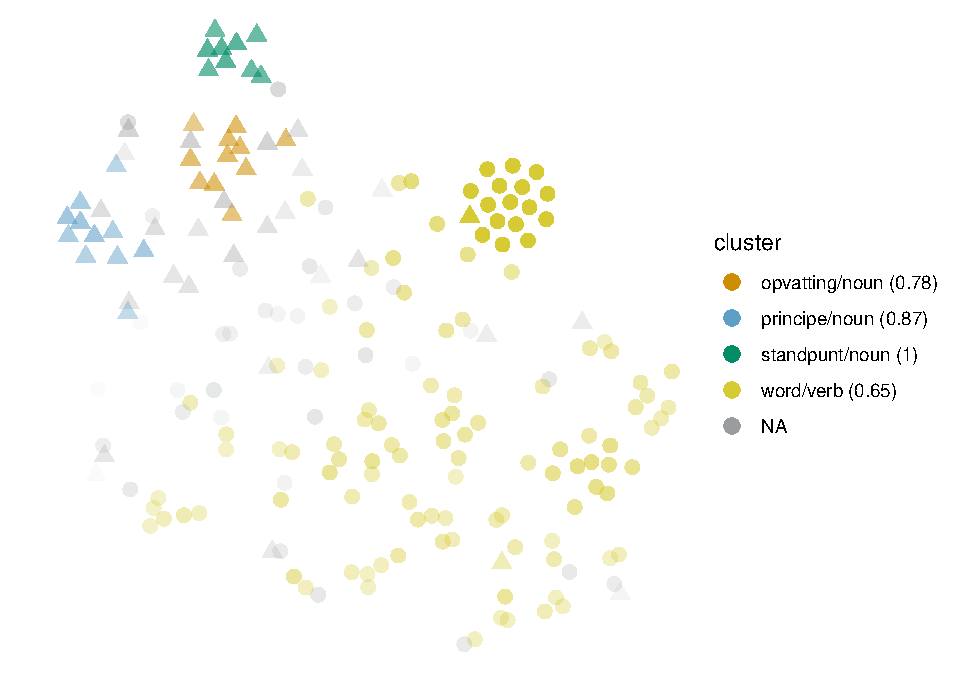
\includegraphics{phdThesis_files/figure-latex/huldigen-1.pdf}
\caption{\label{fig:huldigen}Cloud of \emph{huldigen}.}
\end{figure}

\hypertarget{part-of-a-sense}{%
\subsection{Part of a sense}\label{part-of-a-sense}}

In models that tend to have diffuse clusters, we might have a cluster that holds itself together for unclear reasons and yet represents a part of a sense fairly well. This is certainly not a frequent co-occurrence, but it might indicate that there is a sense-related organization in space, that is however not strong enough to stand out as a defined cluster.

In our data, we find this in the ``best'' medoid of \emph{hoop}, where the `heap' tokens, united by \emph{een}, form a rather diffuse island, slightly separated from the `hope' tokens (Figure \ref{fig:hoop}). In spite of this visually clear separation made by t-SNE, HDBSCAN only manages to capture patches in the form of weak clusters. One such cluster captures all the `heap' tokens that are clustered, but a number of them are lost as noise. Because of this, \emph{een} has a perfect recall for this cluster but a very low precision; meanwhile, the rest of the context words involved form no pattern at all.



\begin{figure}
\centering
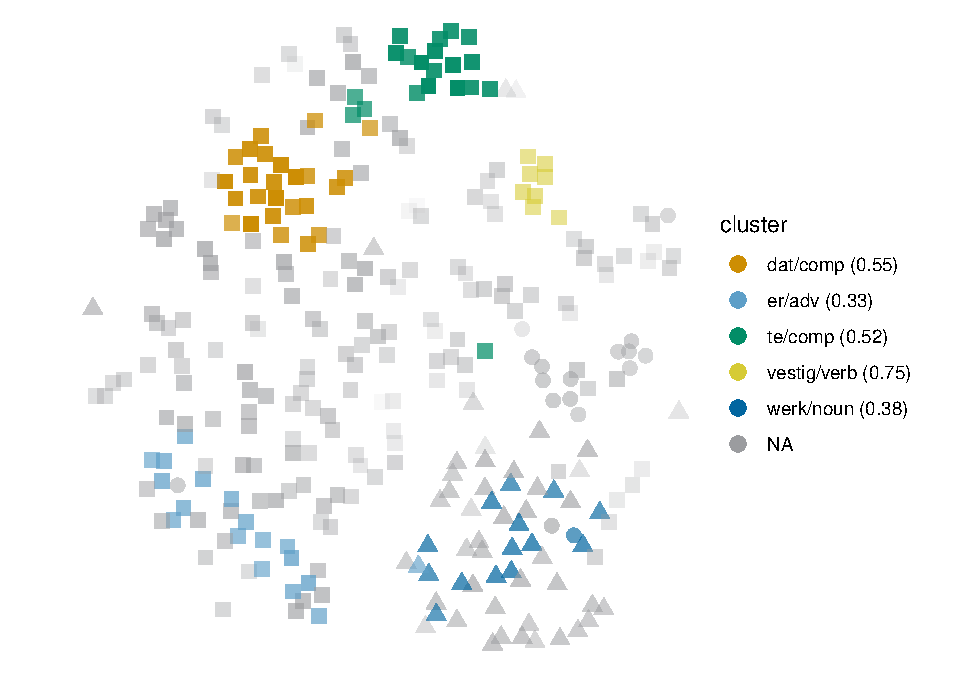
\includegraphics{phdThesis_files/figure-latex/hoop-1.pdf}
\caption{\label{fig:hoop}Cloud of \emph{hoop}.}
\end{figure}

\hypertarget{summary}{%
\section{Summary}\label{summary}}

\hypertarget{no-sky-fits-all}{%
\chapter{No sky fits all}\label{no-sky-fits-all}}

\hypertarget{part-conclusion}{%
\part{Conclusion}\label{part-conclusion}}

\hypertarget{cloudspotters-guide}{%
\chapter{Cloudspotter's guide}\label{cloudspotters-guide}}

{[}General tips and so on{]}

\hypertarget{avenues-for-further-research}{%
\chapter{Avenues for further research}\label{avenues-for-further-research}}

\hypertarget{conclusion}{%
\chapter{Conclusion}\label{conclusion}}

\hypertarget{refs}{}
\begin{CSLReferences}{0}{0}
\end{CSLReferences}

\hypertarget{appendix-appendix}{%
\appendix}


\hypertarget{definitions}{%
\chapter{Definitions}\label{definitions}}

\hypertarget{hoopvol}{%
\section*{hoopvol}\label{hoopvol}}
\addcontentsline{toc}{section}{hoopvol}

\providecommand{\docline}[3]{\noalign{\global\setlength{\arrayrulewidth}{#1}}\arrayrulecolor[HTML]{#2}\cline{#3}}

\setlength{\tabcolsep}{2pt}

\renewcommand*{\arraystretch}{1.5}

\begin{longtable}[c]{|p{0.99in}|p{9.20in}|p{10.15in}}



\hhline{>{\arrayrulecolor[HTML]{666666}\global\arrayrulewidth=2pt}->{\arrayrulecolor[HTML]{666666}\global\arrayrulewidth=2pt}->{\arrayrulecolor[HTML]{666666}\global\arrayrulewidth=2pt}-}

\multicolumn{1}{!{\color[HTML]{000000}\vrule width 0pt}>{\raggedright}p{\dimexpr 0.99in+0\tabcolsep+0\arrayrulewidth}}{\fontsize{11}{11}\selectfont{\textcolor[HTML]{000000}{\global\setmainfont{Arial}sense}}} & \multicolumn{1}{!{\color[HTML]{000000}\vrule width 0pt}>{\raggedright}p{\dimexpr 9.2in+0\tabcolsep+0\arrayrulewidth}}{\fontsize{11}{11}\selectfont{\textcolor[HTML]{000000}{\global\setmainfont{Arial}Dutch}}} & \multicolumn{1}{!{\color[HTML]{000000}\vrule width 0pt}>{\raggedright}p{\dimexpr 10.15in+0\tabcolsep+0\arrayrulewidth}!{\color[HTML]{000000}\vrule width 0pt}}{\fontsize{11}{11}\selectfont{\textcolor[HTML]{000000}{\global\setmainfont{Arial}English}}} \\

\noalign{\global\setlength{\arrayrulewidth}{2pt}}\arrayrulecolor[HTML]{666666}\cline{1-3}

\endfirsthead

\hhline{>{\arrayrulecolor[HTML]{666666}\global\arrayrulewidth=2pt}->{\arrayrulecolor[HTML]{666666}\global\arrayrulewidth=2pt}->{\arrayrulecolor[HTML]{666666}\global\arrayrulewidth=2pt}-}

\multicolumn{1}{!{\color[HTML]{000000}\vrule width 0pt}>{\raggedright}p{\dimexpr 0.99in+0\tabcolsep+0\arrayrulewidth}}{\fontsize{11}{11}\selectfont{\textcolor[HTML]{000000}{\global\setmainfont{Arial}sense}}} & \multicolumn{1}{!{\color[HTML]{000000}\vrule width 0pt}>{\raggedright}p{\dimexpr 9.2in+0\tabcolsep+0\arrayrulewidth}}{\fontsize{11}{11}\selectfont{\textcolor[HTML]{000000}{\global\setmainfont{Arial}Dutch}}} & \multicolumn{1}{!{\color[HTML]{000000}\vrule width 0pt}>{\raggedright}p{\dimexpr 10.15in+0\tabcolsep+0\arrayrulewidth}!{\color[HTML]{000000}\vrule width 0pt}}{\fontsize{11}{11}\selectfont{\textcolor[HTML]{000000}{\global\setmainfont{Arial}English}}} \\

\noalign{\global\setlength{\arrayrulewidth}{2pt}}\arrayrulecolor[HTML]{666666}\cline{1-3}\endhead



\multicolumn{1}{!{\color[HTML]{000000}\vrule width 0pt}>{\raggedright}p{\dimexpr 0.99in+0\tabcolsep+0\arrayrulewidth}}{\fontsize{11}{11}\selectfont{\textcolor[HTML]{000000}{\global\setmainfont{Arial}hoopvol\_1}}} & \multicolumn{1}{!{\color[HTML]{000000}\vrule width 0pt}>{\raggedright}p{\dimexpr 9.2in+0\tabcolsep+0\arrayrulewidth}}{\fontsize{11}{11}\selectfont{\textcolor[HTML]{000000}{\global\setmainfont{Arial}(van personen, uitingen, gedragingen etc.) blijk gevend van hoop, vol hoop, optimistisch}}\fontsize{11}{11}\selectfont{\textcolor[HTML]{000000}{\global\setmainfont{Arial}: }}\fontsize{10}{10}\selectfont{\textcolor[HTML]{000000}{\global\setmainfont{Arial}\textit{een hoopvolle stemming, dat stemt mij hoopvol}}}} & \multicolumn{1}{!{\color[HTML]{000000}\vrule width 0pt}>{\raggedright}p{\dimexpr 10.15in+0\tabcolsep+0\arrayrulewidth}!{\color[HTML]{000000}\vrule width 0pt}}{\fontsize{11}{11}\selectfont{\textcolor[HTML]{000000}{\global\setmainfont{Arial}(of people, expressions, behaviors, etc.) giving an impression of hope, full of hope, optimistic}}\fontsize{11}{11}\selectfont{\textcolor[HTML]{000000}{\global\setmainfont{Arial}: }}\fontsize{10}{10}\selectfont{\textcolor[HTML]{000000}{\global\setmainfont{Arial}\textit{a hopeful mood, that brings me hope (makes me hopeful)}}}} \\





\multicolumn{1}{!{\color[HTML]{000000}\vrule width 0pt}>{\raggedright}p{\dimexpr 0.99in+0\tabcolsep+0\arrayrulewidth}}{\fontsize{11}{11}\selectfont{\textcolor[HTML]{000000}{\global\setmainfont{Arial}hoopvol\_2}}} & \multicolumn{1}{!{\color[HTML]{000000}\vrule width 0pt}>{\raggedright}p{\dimexpr 9.2in+0\tabcolsep+0\arrayrulewidth}}{\fontsize{11}{11}\selectfont{\textcolor[HTML]{000000}{\global\setmainfont{Arial}reden tot hoop gevend, beloftevol}}\fontsize{11}{11}\selectfont{\textcolor[HTML]{000000}{\global\setmainfont{Arial}: }}\fontsize{10}{10}\selectfont{\textcolor[HTML]{000000}{\global\setmainfont{Arial}\textit{hoopvolle perspectieven}}}} & \multicolumn{1}{!{\color[HTML]{000000}\vrule width 0pt}>{\raggedright}p{\dimexpr 10.15in+0\tabcolsep+0\arrayrulewidth}!{\color[HTML]{000000}\vrule width 0pt}}{\fontsize{11}{11}\selectfont{\textcolor[HTML]{000000}{\global\setmainfont{Arial}giving reason for hope, promising}}\fontsize{11}{11}\selectfont{\textcolor[HTML]{000000}{\global\setmainfont{Arial}: }}\fontsize{10}{10}\selectfont{\textcolor[HTML]{000000}{\global\setmainfont{Arial}\textit{hopeful perspectives}}}} \\

\noalign{\global\setlength{\arrayrulewidth}{2pt}}\arrayrulecolor[HTML]{666666}\cline{1-3}

\end{longtable}

\hypertarget{geestig}{%
\section*{geestig}\label{geestig}}
\addcontentsline{toc}{section}{geestig}

\providecommand{\docline}[3]{\noalign{\global\setlength{\arrayrulewidth}{#1}}\arrayrulecolor[HTML]{#2}\cline{#3}}

\setlength{\tabcolsep}{2pt}

\renewcommand*{\arraystretch}{1.5}

\begin{longtable}[c]{|p{0.95in}|p{9.98in}|p{7.80in}}



\hhline{>{\arrayrulecolor[HTML]{666666}\global\arrayrulewidth=2pt}->{\arrayrulecolor[HTML]{666666}\global\arrayrulewidth=2pt}->{\arrayrulecolor[HTML]{666666}\global\arrayrulewidth=2pt}-}

\multicolumn{1}{!{\color[HTML]{000000}\vrule width 0pt}>{\raggedright}p{\dimexpr 0.95in+0\tabcolsep+0\arrayrulewidth}}{\fontsize{11}{11}\selectfont{\textcolor[HTML]{000000}{\global\setmainfont{Arial}sense}}} & \multicolumn{1}{!{\color[HTML]{000000}\vrule width 0pt}>{\raggedright}p{\dimexpr 9.98in+0\tabcolsep+0\arrayrulewidth}}{\fontsize{11}{11}\selectfont{\textcolor[HTML]{000000}{\global\setmainfont{Arial}Dutch}}} & \multicolumn{1}{!{\color[HTML]{000000}\vrule width 0pt}>{\raggedright}p{\dimexpr 7.8in+0\tabcolsep+0\arrayrulewidth}!{\color[HTML]{000000}\vrule width 0pt}}{\fontsize{11}{11}\selectfont{\textcolor[HTML]{000000}{\global\setmainfont{Arial}English}}} \\

\noalign{\global\setlength{\arrayrulewidth}{2pt}}\arrayrulecolor[HTML]{666666}\cline{1-3}

\endfirsthead

\hhline{>{\arrayrulecolor[HTML]{666666}\global\arrayrulewidth=2pt}->{\arrayrulecolor[HTML]{666666}\global\arrayrulewidth=2pt}->{\arrayrulecolor[HTML]{666666}\global\arrayrulewidth=2pt}-}

\multicolumn{1}{!{\color[HTML]{000000}\vrule width 0pt}>{\raggedright}p{\dimexpr 0.95in+0\tabcolsep+0\arrayrulewidth}}{\fontsize{11}{11}\selectfont{\textcolor[HTML]{000000}{\global\setmainfont{Arial}sense}}} & \multicolumn{1}{!{\color[HTML]{000000}\vrule width 0pt}>{\raggedright}p{\dimexpr 9.98in+0\tabcolsep+0\arrayrulewidth}}{\fontsize{11}{11}\selectfont{\textcolor[HTML]{000000}{\global\setmainfont{Arial}Dutch}}} & \multicolumn{1}{!{\color[HTML]{000000}\vrule width 0pt}>{\raggedright}p{\dimexpr 7.8in+0\tabcolsep+0\arrayrulewidth}!{\color[HTML]{000000}\vrule width 0pt}}{\fontsize{11}{11}\selectfont{\textcolor[HTML]{000000}{\global\setmainfont{Arial}English}}} \\

\noalign{\global\setlength{\arrayrulewidth}{2pt}}\arrayrulecolor[HTML]{666666}\cline{1-3}\endhead



\multicolumn{1}{!{\color[HTML]{000000}\vrule width 0pt}>{\raggedright}p{\dimexpr 0.95in+0\tabcolsep+0\arrayrulewidth}}{\fontsize{11}{11}\selectfont{\textcolor[HTML]{000000}{\global\setmainfont{Arial}geestig\_1}}} & \multicolumn{1}{!{\color[HTML]{000000}\vrule width 0pt}>{\raggedright}p{\dimexpr 9.98in+0\tabcolsep+0\arrayrulewidth}}{\fontsize{11}{11}\selectfont{\textcolor[HTML]{000000}{\global\setmainfont{Arial}scherpzinnig en humoristisch van aard}}\fontsize{11}{11}\selectfont{\textcolor[HTML]{000000}{\global\setmainfont{Arial}: }}\fontsize{10}{10}\selectfont{\textcolor[HTML]{000000}{\global\setmainfont{Arial}\textit{een geestige collega}}}} & \multicolumn{1}{!{\color[HTML]{000000}\vrule width 0pt}>{\raggedright}p{\dimexpr 7.8in+0\tabcolsep+0\arrayrulewidth}!{\color[HTML]{000000}\vrule width 0pt}}{\fontsize{11}{11}\selectfont{\textcolor[HTML]{000000}{\global\setmainfont{Arial}of witty and humoristic nature}}\fontsize{11}{11}\selectfont{\textcolor[HTML]{000000}{\global\setmainfont{Arial}: }}\fontsize{10}{10}\selectfont{\textcolor[HTML]{000000}{\global\setmainfont{Arial}\textit{a witty colleague}}}} \\





\multicolumn{1}{!{\color[HTML]{000000}\vrule width 0pt}>{\raggedright}p{\dimexpr 0.95in+0\tabcolsep+0\arrayrulewidth}}{\fontsize{11}{11}\selectfont{\textcolor[HTML]{000000}{\global\setmainfont{Arial}geestig\_2}}} & \multicolumn{1}{!{\color[HTML]{000000}\vrule width 0pt}>{\raggedright}p{\dimexpr 9.98in+0\tabcolsep+0\arrayrulewidth}}{\fontsize{11}{11}\selectfont{\textcolor[HTML]{000000}{\global\setmainfont{Arial}blijk gevend van, uitdrukking gevend aan, gekenmerkt door scherpzinnigheid en humor}}\fontsize{11}{11}\selectfont{\textcolor[HTML]{000000}{\global\setmainfont{Arial}: }}\fontsize{10}{10}\selectfont{\textcolor[HTML]{000000}{\global\setmainfont{Arial}\textit{een geestig boek, een geestige blik, een geestige opmerking}}}} & \multicolumn{1}{!{\color[HTML]{000000}\vrule width 0pt}>{\raggedright}p{\dimexpr 7.8in+0\tabcolsep+0\arrayrulewidth}!{\color[HTML]{000000}\vrule width 0pt}}{\fontsize{11}{11}\selectfont{\textcolor[HTML]{000000}{\global\setmainfont{Arial}giving an impression of, expressing, characterized by wittiness and humor}}\fontsize{11}{11}\selectfont{\textcolor[HTML]{000000}{\global\setmainfont{Arial}: }}\fontsize{10}{10}\selectfont{\textcolor[HTML]{000000}{\global\setmainfont{Arial}\textit{a witty book, a witty look, a witty remark}}}} \\





\multicolumn{1}{!{\color[HTML]{000000}\vrule width 0pt}>{\raggedright}p{\dimexpr 0.95in+0\tabcolsep+0\arrayrulewidth}}{\fontsize{11}{11}\selectfont{\textcolor[HTML]{000000}{\global\setmainfont{Arial}geestig\_3}}} & \multicolumn{1}{!{\color[HTML]{000000}\vrule width 0pt}>{\raggedright}p{\dimexpr 9.98in+0\tabcolsep+0\arrayrulewidth}}{\fontsize{11}{11}\selectfont{\textcolor[HTML]{000000}{\global\setmainfont{Arial}}}\fontsize{11}{11}\selectfont{\textcolor[HTML]{000000}{\global\setmainfont{Arial}: }}\fontsize{10}{10}\selectfont{\textcolor[HTML]{000000}{\global\setmainfont{Arial}\textit{}}}} & \multicolumn{1}{!{\color[HTML]{000000}\vrule width 0pt}>{\raggedright}p{\dimexpr 7.8in+0\tabcolsep+0\arrayrulewidth}!{\color[HTML]{000000}\vrule width 0pt}}{\fontsize{11}{11}\selectfont{\textcolor[HTML]{000000}{\global\setmainfont{Arial}be perceived as funny (and witty?)}}\fontsize{11}{11}\selectfont{\textcolor[HTML]{000000}{\global\setmainfont{Arial}: }}\fontsize{10}{10}\selectfont{\textcolor[HTML]{000000}{\global\setmainfont{Arial}\textit{I find this funny}}}} \\

\noalign{\global\setlength{\arrayrulewidth}{2pt}}\arrayrulecolor[HTML]{666666}\cline{1-3}

\end{longtable}

\hypertarget{hachelijk}{%
\section*{hachelijk}\label{hachelijk}}
\addcontentsline{toc}{section}{hachelijk}

\providecommand{\docline}[3]{\noalign{\global\setlength{\arrayrulewidth}{#1}}\arrayrulecolor[HTML]{#2}\cline{#3}}

\setlength{\tabcolsep}{2pt}

\renewcommand*{\arraystretch}{1.5}

\begin{longtable}[c]{|p{1.05in}|p{6.02in}|p{5.96in}}



\hhline{>{\arrayrulecolor[HTML]{666666}\global\arrayrulewidth=2pt}->{\arrayrulecolor[HTML]{666666}\global\arrayrulewidth=2pt}->{\arrayrulecolor[HTML]{666666}\global\arrayrulewidth=2pt}-}

\multicolumn{1}{!{\color[HTML]{000000}\vrule width 0pt}>{\raggedright}p{\dimexpr 1.05in+0\tabcolsep+0\arrayrulewidth}}{\fontsize{11}{11}\selectfont{\textcolor[HTML]{000000}{\global\setmainfont{Arial}sense}}} & \multicolumn{1}{!{\color[HTML]{000000}\vrule width 0pt}>{\raggedright}p{\dimexpr 6.02in+0\tabcolsep+0\arrayrulewidth}}{\fontsize{11}{11}\selectfont{\textcolor[HTML]{000000}{\global\setmainfont{Arial}Dutch}}} & \multicolumn{1}{!{\color[HTML]{000000}\vrule width 0pt}>{\raggedright}p{\dimexpr 5.96in+0\tabcolsep+0\arrayrulewidth}!{\color[HTML]{000000}\vrule width 0pt}}{\fontsize{11}{11}\selectfont{\textcolor[HTML]{000000}{\global\setmainfont{Arial}English}}} \\

\noalign{\global\setlength{\arrayrulewidth}{2pt}}\arrayrulecolor[HTML]{666666}\cline{1-3}

\endfirsthead

\hhline{>{\arrayrulecolor[HTML]{666666}\global\arrayrulewidth=2pt}->{\arrayrulecolor[HTML]{666666}\global\arrayrulewidth=2pt}->{\arrayrulecolor[HTML]{666666}\global\arrayrulewidth=2pt}-}

\multicolumn{1}{!{\color[HTML]{000000}\vrule width 0pt}>{\raggedright}p{\dimexpr 1.05in+0\tabcolsep+0\arrayrulewidth}}{\fontsize{11}{11}\selectfont{\textcolor[HTML]{000000}{\global\setmainfont{Arial}sense}}} & \multicolumn{1}{!{\color[HTML]{000000}\vrule width 0pt}>{\raggedright}p{\dimexpr 6.02in+0\tabcolsep+0\arrayrulewidth}}{\fontsize{11}{11}\selectfont{\textcolor[HTML]{000000}{\global\setmainfont{Arial}Dutch}}} & \multicolumn{1}{!{\color[HTML]{000000}\vrule width 0pt}>{\raggedright}p{\dimexpr 5.96in+0\tabcolsep+0\arrayrulewidth}!{\color[HTML]{000000}\vrule width 0pt}}{\fontsize{11}{11}\selectfont{\textcolor[HTML]{000000}{\global\setmainfont{Arial}English}}} \\

\noalign{\global\setlength{\arrayrulewidth}{2pt}}\arrayrulecolor[HTML]{666666}\cline{1-3}\endhead



\multicolumn{1}{!{\color[HTML]{000000}\vrule width 0pt}>{\raggedright}p{\dimexpr 1.05in+0\tabcolsep+0\arrayrulewidth}}{\fontsize{11}{11}\selectfont{\textcolor[HTML]{000000}{\global\setmainfont{Arial}hachelijk\_1}}} & \multicolumn{1}{!{\color[HTML]{000000}\vrule width 0pt}>{\raggedright}p{\dimexpr 6.02in+0\tabcolsep+0\arrayrulewidth}}{\fontsize{11}{11}\selectfont{\textcolor[HTML]{000000}{\global\setmainfont{Arial}met kans op een ongunstige afloop, (potentieel) gevaarlijk}}\fontsize{11}{11}\selectfont{\textcolor[HTML]{000000}{\global\setmainfont{Arial}: }}\fontsize{10}{10}\selectfont{\textcolor[HTML]{000000}{\global\setmainfont{Arial}\textit{een hachelijke onderneming}}}} & \multicolumn{1}{!{\color[HTML]{000000}\vrule width 0pt}>{\raggedright}p{\dimexpr 5.96in+0\tabcolsep+0\arrayrulewidth}!{\color[HTML]{000000}\vrule width 0pt}}{\fontsize{11}{11}\selectfont{\textcolor[HTML]{000000}{\global\setmainfont{Arial}with chances of unfavorable outcome, (potentially) dangerous}}\fontsize{11}{11}\selectfont{\textcolor[HTML]{000000}{\global\setmainfont{Arial}: }}\fontsize{10}{10}\selectfont{\textcolor[HTML]{000000}{\global\setmainfont{Arial}\textit{a dangerous enterprise}}}} \\





\multicolumn{1}{!{\color[HTML]{000000}\vrule width 0pt}>{\raggedright}p{\dimexpr 1.05in+0\tabcolsep+0\arrayrulewidth}}{\fontsize{11}{11}\selectfont{\textcolor[HTML]{000000}{\global\setmainfont{Arial}hachelijk\_2}}} & \multicolumn{1}{!{\color[HTML]{000000}\vrule width 0pt}>{\raggedright}p{\dimexpr 6.02in+0\tabcolsep+0\arrayrulewidth}}{\fontsize{11}{11}\selectfont{\textcolor[HTML]{000000}{\global\setmainfont{Arial}(reëel) gevaarlijk, netelig, kritiek, benard}}\fontsize{11}{11}\selectfont{\textcolor[HTML]{000000}{\global\setmainfont{Arial}: }}\fontsize{10}{10}\selectfont{\textcolor[HTML]{000000}{\global\setmainfont{Arial}\textit{een hachelijke situatie}}}} & \multicolumn{1}{!{\color[HTML]{000000}\vrule width 0pt}>{\raggedright}p{\dimexpr 5.96in+0\tabcolsep+0\arrayrulewidth}!{\color[HTML]{000000}\vrule width 0pt}}{\fontsize{11}{11}\selectfont{\textcolor[HTML]{000000}{\global\setmainfont{Arial}(really) dangerous, trick, critical, dire}}\fontsize{11}{11}\selectfont{\textcolor[HTML]{000000}{\global\setmainfont{Arial}: }}\fontsize{10}{10}\selectfont{\textcolor[HTML]{000000}{\global\setmainfont{Arial}\textit{a dangerous situation}}}} \\

\noalign{\global\setlength{\arrayrulewidth}{2pt}}\arrayrulecolor[HTML]{666666}\cline{1-3}

\end{longtable}

\hypertarget{hoekig}{%
\section*{hoekig}\label{hoekig}}
\addcontentsline{toc}{section}{hoekig}

\providecommand{\docline}[3]{\noalign{\global\setlength{\arrayrulewidth}{#1}}\arrayrulecolor[HTML]{#2}\cline{#3}}

\setlength{\tabcolsep}{2pt}

\renewcommand*{\arraystretch}{1.5}

\begin{longtable}[c]{|p{0.91in}|p{7.06in}|p{6.29in}}



\hhline{>{\arrayrulecolor[HTML]{666666}\global\arrayrulewidth=2pt}->{\arrayrulecolor[HTML]{666666}\global\arrayrulewidth=2pt}->{\arrayrulecolor[HTML]{666666}\global\arrayrulewidth=2pt}-}

\multicolumn{1}{!{\color[HTML]{000000}\vrule width 0pt}>{\raggedright}p{\dimexpr 0.91in+0\tabcolsep+0\arrayrulewidth}}{\fontsize{11}{11}\selectfont{\textcolor[HTML]{000000}{\global\setmainfont{Arial}sense}}} & \multicolumn{1}{!{\color[HTML]{000000}\vrule width 0pt}>{\raggedright}p{\dimexpr 7.06in+0\tabcolsep+0\arrayrulewidth}}{\fontsize{11}{11}\selectfont{\textcolor[HTML]{000000}{\global\setmainfont{Arial}Dutch}}} & \multicolumn{1}{!{\color[HTML]{000000}\vrule width 0pt}>{\raggedright}p{\dimexpr 6.29in+0\tabcolsep+0\arrayrulewidth}!{\color[HTML]{000000}\vrule width 0pt}}{\fontsize{11}{11}\selectfont{\textcolor[HTML]{000000}{\global\setmainfont{Arial}English}}} \\

\noalign{\global\setlength{\arrayrulewidth}{2pt}}\arrayrulecolor[HTML]{666666}\cline{1-3}

\endfirsthead

\hhline{>{\arrayrulecolor[HTML]{666666}\global\arrayrulewidth=2pt}->{\arrayrulecolor[HTML]{666666}\global\arrayrulewidth=2pt}->{\arrayrulecolor[HTML]{666666}\global\arrayrulewidth=2pt}-}

\multicolumn{1}{!{\color[HTML]{000000}\vrule width 0pt}>{\raggedright}p{\dimexpr 0.91in+0\tabcolsep+0\arrayrulewidth}}{\fontsize{11}{11}\selectfont{\textcolor[HTML]{000000}{\global\setmainfont{Arial}sense}}} & \multicolumn{1}{!{\color[HTML]{000000}\vrule width 0pt}>{\raggedright}p{\dimexpr 7.06in+0\tabcolsep+0\arrayrulewidth}}{\fontsize{11}{11}\selectfont{\textcolor[HTML]{000000}{\global\setmainfont{Arial}Dutch}}} & \multicolumn{1}{!{\color[HTML]{000000}\vrule width 0pt}>{\raggedright}p{\dimexpr 6.29in+0\tabcolsep+0\arrayrulewidth}!{\color[HTML]{000000}\vrule width 0pt}}{\fontsize{11}{11}\selectfont{\textcolor[HTML]{000000}{\global\setmainfont{Arial}English}}} \\

\noalign{\global\setlength{\arrayrulewidth}{2pt}}\arrayrulecolor[HTML]{666666}\cline{1-3}\endhead



\multicolumn{1}{!{\color[HTML]{000000}\vrule width 0pt}>{\raggedright}p{\dimexpr 0.91in+0\tabcolsep+0\arrayrulewidth}}{\fontsize{11}{11}\selectfont{\textcolor[HTML]{000000}{\global\setmainfont{Arial}hoekig\_1}}} & \multicolumn{1}{!{\color[HTML]{000000}\vrule width 0pt}>{\raggedright}p{\dimexpr 7.06in+0\tabcolsep+0\arrayrulewidth}}{\fontsize{11}{11}\selectfont{\textcolor[HTML]{000000}{\global\setmainfont{Arial}(van voorwerpen, figuren e.d.) met hoeken of scherpe kanten}}\fontsize{11}{11}\selectfont{\textcolor[HTML]{000000}{\global\setmainfont{Arial}: }}\fontsize{10}{10}\selectfont{\textcolor[HTML]{000000}{\global\setmainfont{Arial}\textit{een hoekige tekening, een hoekig gezicht}}}} & \multicolumn{1}{!{\color[HTML]{000000}\vrule width 0pt}>{\raggedright}p{\dimexpr 6.29in+0\tabcolsep+0\arrayrulewidth}!{\color[HTML]{000000}\vrule width 0pt}}{\fontsize{11}{11}\selectfont{\textcolor[HTML]{000000}{\global\setmainfont{Arial}(of objects, figures, etc.) with angles or sharp edges}}\fontsize{11}{11}\selectfont{\textcolor[HTML]{000000}{\global\setmainfont{Arial}: }}\fontsize{10}{10}\selectfont{\textcolor[HTML]{000000}{\global\setmainfont{Arial}\textit{an angulous drawing, an angulous face}}}} \\





\multicolumn{1}{!{\color[HTML]{000000}\vrule width 0pt}>{\raggedright}p{\dimexpr 0.91in+0\tabcolsep+0\arrayrulewidth}}{\fontsize{11}{11}\selectfont{\textcolor[HTML]{000000}{\global\setmainfont{Arial}hoekig\_2}}} & \multicolumn{1}{!{\color[HTML]{000000}\vrule width 0pt}>{\raggedright}p{\dimexpr 7.06in+0\tabcolsep+0\arrayrulewidth}}{\fontsize{11}{11}\selectfont{\textcolor[HTML]{000000}{\global\setmainfont{Arial}(van bewegingen, ritmes e.d.) niet vloeiend}}\fontsize{11}{11}\selectfont{\textcolor[HTML]{000000}{\global\setmainfont{Arial}: }}\fontsize{10}{10}\selectfont{\textcolor[HTML]{000000}{\global\setmainfont{Arial}\textit{een hoekig melodietje}}}} & \multicolumn{1}{!{\color[HTML]{000000}\vrule width 0pt}>{\raggedright}p{\dimexpr 6.29in+0\tabcolsep+0\arrayrulewidth}!{\color[HTML]{000000}\vrule width 0pt}}{\fontsize{11}{11}\selectfont{\textcolor[HTML]{000000}{\global\setmainfont{Arial}(of movements, rhythms, etc.) not fluent}}\fontsize{11}{11}\selectfont{\textcolor[HTML]{000000}{\global\setmainfont{Arial}: }}\fontsize{10}{10}\selectfont{\textcolor[HTML]{000000}{\global\setmainfont{Arial}\textit{a broken melody}}}} \\





\multicolumn{1}{!{\color[HTML]{000000}\vrule width 0pt}>{\raggedright}p{\dimexpr 0.91in+0\tabcolsep+0\arrayrulewidth}}{\fontsize{11}{11}\selectfont{\textcolor[HTML]{000000}{\global\setmainfont{Arial}hoekig\_3}}} & \multicolumn{1}{!{\color[HTML]{000000}\vrule width 0pt}>{\raggedright}p{\dimexpr 7.06in+0\tabcolsep+0\arrayrulewidth}}{\fontsize{11}{11}\selectfont{\textcolor[HTML]{000000}{\global\setmainfont{Arial}(van personen) houterig, stijf, onhandig in de omgang}}\fontsize{11}{11}\selectfont{\textcolor[HTML]{000000}{\global\setmainfont{Arial}: }}\fontsize{10}{10}\selectfont{\textcolor[HTML]{000000}{\global\setmainfont{Arial}\textit{een hoekig karakter}}}} & \multicolumn{1}{!{\color[HTML]{000000}\vrule width 0pt}>{\raggedright}p{\dimexpr 6.29in+0\tabcolsep+0\arrayrulewidth}!{\color[HTML]{000000}\vrule width 0pt}}{\fontsize{11}{11}\selectfont{\textcolor[HTML]{000000}{\global\setmainfont{Arial}(of people) rigid, stiff, clumsy}}\fontsize{11}{11}\selectfont{\textcolor[HTML]{000000}{\global\setmainfont{Arial}: }}\fontsize{10}{10}\selectfont{\textcolor[HTML]{000000}{\global\setmainfont{Arial}\textit{a clumsy character}}}} \\

\noalign{\global\setlength{\arrayrulewidth}{2pt}}\arrayrulecolor[HTML]{666666}\cline{1-3}

\end{longtable}

\hypertarget{dof}{%
\section*{dof}\label{dof}}
\addcontentsline{toc}{section}{dof}

\providecommand{\docline}[3]{\noalign{\global\setlength{\arrayrulewidth}{#1}}\arrayrulecolor[HTML]{#2}\cline{#3}}

\setlength{\tabcolsep}{2pt}

\renewcommand*{\arraystretch}{1.5}

\begin{longtable}[c]{|p{0.69in}|p{7.50in}|p{6.08in}}



\hhline{>{\arrayrulecolor[HTML]{666666}\global\arrayrulewidth=2pt}->{\arrayrulecolor[HTML]{666666}\global\arrayrulewidth=2pt}->{\arrayrulecolor[HTML]{666666}\global\arrayrulewidth=2pt}-}

\multicolumn{1}{!{\color[HTML]{000000}\vrule width 0pt}>{\raggedright}p{\dimexpr 0.69in+0\tabcolsep+0\arrayrulewidth}}{\fontsize{11}{11}\selectfont{\textcolor[HTML]{000000}{\global\setmainfont{Arial}sense}}} & \multicolumn{1}{!{\color[HTML]{000000}\vrule width 0pt}>{\raggedright}p{\dimexpr 7.5in+0\tabcolsep+0\arrayrulewidth}}{\fontsize{11}{11}\selectfont{\textcolor[HTML]{000000}{\global\setmainfont{Arial}Dutch}}} & \multicolumn{1}{!{\color[HTML]{000000}\vrule width 0pt}>{\raggedright}p{\dimexpr 6.08in+0\tabcolsep+0\arrayrulewidth}!{\color[HTML]{000000}\vrule width 0pt}}{\fontsize{11}{11}\selectfont{\textcolor[HTML]{000000}{\global\setmainfont{Arial}English}}} \\

\noalign{\global\setlength{\arrayrulewidth}{2pt}}\arrayrulecolor[HTML]{666666}\cline{1-3}

\endfirsthead

\hhline{>{\arrayrulecolor[HTML]{666666}\global\arrayrulewidth=2pt}->{\arrayrulecolor[HTML]{666666}\global\arrayrulewidth=2pt}->{\arrayrulecolor[HTML]{666666}\global\arrayrulewidth=2pt}-}

\multicolumn{1}{!{\color[HTML]{000000}\vrule width 0pt}>{\raggedright}p{\dimexpr 0.69in+0\tabcolsep+0\arrayrulewidth}}{\fontsize{11}{11}\selectfont{\textcolor[HTML]{000000}{\global\setmainfont{Arial}sense}}} & \multicolumn{1}{!{\color[HTML]{000000}\vrule width 0pt}>{\raggedright}p{\dimexpr 7.5in+0\tabcolsep+0\arrayrulewidth}}{\fontsize{11}{11}\selectfont{\textcolor[HTML]{000000}{\global\setmainfont{Arial}Dutch}}} & \multicolumn{1}{!{\color[HTML]{000000}\vrule width 0pt}>{\raggedright}p{\dimexpr 6.08in+0\tabcolsep+0\arrayrulewidth}!{\color[HTML]{000000}\vrule width 0pt}}{\fontsize{11}{11}\selectfont{\textcolor[HTML]{000000}{\global\setmainfont{Arial}English}}} \\

\noalign{\global\setlength{\arrayrulewidth}{2pt}}\arrayrulecolor[HTML]{666666}\cline{1-3}\endhead



\multicolumn{1}{!{\color[HTML]{000000}\vrule width 0pt}>{\raggedright}p{\dimexpr 0.69in+0\tabcolsep+0\arrayrulewidth}}{\fontsize{11}{11}\selectfont{\textcolor[HTML]{000000}{\global\setmainfont{Arial}dof\_1}}} & \multicolumn{1}{!{\color[HTML]{000000}\vrule width 0pt}>{\raggedright}p{\dimexpr 7.5in+0\tabcolsep+0\arrayrulewidth}}{\fontsize{11}{11}\selectfont{\textcolor[HTML]{000000}{\global\setmainfont{Arial}(van kleuren en zichtbare dingen) mat, zonder glans, vaal}}\fontsize{11}{11}\selectfont{\textcolor[HTML]{000000}{\global\setmainfont{Arial}: }}\fontsize{10}{10}\selectfont{\textcolor[HTML]{000000}{\global\setmainfont{Arial}\textit{een doffe blik}}}} & \multicolumn{1}{!{\color[HTML]{000000}\vrule width 0pt}>{\raggedright}p{\dimexpr 6.08in+0\tabcolsep+0\arrayrulewidth}!{\color[HTML]{000000}\vrule width 0pt}}{\fontsize{11}{11}\selectfont{\textcolor[HTML]{000000}{\global\setmainfont{Arial}(of colours and visible things) matte, without shine, pale}}\fontsize{11}{11}\selectfont{\textcolor[HTML]{000000}{\global\setmainfont{Arial}: }}\fontsize{10}{10}\selectfont{\textcolor[HTML]{000000}{\global\setmainfont{Arial}\textit{a dull gaze}}}} \\





\multicolumn{1}{!{\color[HTML]{000000}\vrule width 0pt}>{\raggedright}p{\dimexpr 0.69in+0\tabcolsep+0\arrayrulewidth}}{\fontsize{11}{11}\selectfont{\textcolor[HTML]{000000}{\global\setmainfont{Arial}dof\_2}}} & \multicolumn{1}{!{\color[HTML]{000000}\vrule width 0pt}>{\raggedright}p{\dimexpr 7.5in+0\tabcolsep+0\arrayrulewidth}}{\fontsize{11}{11}\selectfont{\textcolor[HTML]{000000}{\global\setmainfont{Arial}(van geluiden) niet luid of scherp, onderdrukt, gesmoord}}\fontsize{11}{11}\selectfont{\textcolor[HTML]{000000}{\global\setmainfont{Arial}: }}\fontsize{10}{10}\selectfont{\textcolor[HTML]{000000}{\global\setmainfont{Arial}\textit{een doffe kreet}}}} & \multicolumn{1}{!{\color[HTML]{000000}\vrule width 0pt}>{\raggedright}p{\dimexpr 6.08in+0\tabcolsep+0\arrayrulewidth}!{\color[HTML]{000000}\vrule width 0pt}}{\fontsize{11}{11}\selectfont{\textcolor[HTML]{000000}{\global\setmainfont{Arial}(of sounds) not loud or sharp, suppressed, smothered}}\fontsize{11}{11}\selectfont{\textcolor[HTML]{000000}{\global\setmainfont{Arial}: }}\fontsize{10}{10}\selectfont{\textcolor[HTML]{000000}{\global\setmainfont{Arial}\textit{a dull cry}}}} \\





\multicolumn{1}{!{\color[HTML]{000000}\vrule width 0pt}>{\raggedright}p{\dimexpr 0.69in+0\tabcolsep+0\arrayrulewidth}}{\fontsize{11}{11}\selectfont{\textcolor[HTML]{000000}{\global\setmainfont{Arial}dof\_3}}} & \multicolumn{1}{!{\color[HTML]{000000}\vrule width 0pt}>{\raggedright}p{\dimexpr 7.5in+0\tabcolsep+0\arrayrulewidth}}{\fontsize{11}{11}\selectfont{\textcolor[HTML]{000000}{\global\setmainfont{Arial}(van personen, gevoelens e.d.) niet opgewekt, lusteloos, zonder energie}}\fontsize{11}{11}\selectfont{\textcolor[HTML]{000000}{\global\setmainfont{Arial}: }}\fontsize{10}{10}\selectfont{\textcolor[HTML]{000000}{\global\setmainfont{Arial}\textit{doffe onverschilligheid, doffe ellende}}}} & \multicolumn{1}{!{\color[HTML]{000000}\vrule width 0pt}>{\raggedright}p{\dimexpr 6.08in+0\tabcolsep+0\arrayrulewidth}!{\color[HTML]{000000}\vrule width 0pt}}{\fontsize{11}{11}\selectfont{\textcolor[HTML]{000000}{\global\setmainfont{Arial}(of people, feelings, etc.) not cheerful, apathetic, without energy}}\fontsize{11}{11}\selectfont{\textcolor[HTML]{000000}{\global\setmainfont{Arial}: }}\fontsize{10}{10}\selectfont{\textcolor[HTML]{000000}{\global\setmainfont{Arial}\textit{dull apathy, dull misery}}}} \\





\multicolumn{1}{!{\color[HTML]{000000}\vrule width 0pt}>{\raggedright}p{\dimexpr 0.69in+0\tabcolsep+0\arrayrulewidth}}{\fontsize{11}{11}\selectfont{\textcolor[HTML]{000000}{\global\setmainfont{Arial}dof\_4}}} & \multicolumn{1}{!{\color[HTML]{000000}\vrule width 0pt}>{\raggedright}p{\dimexpr 7.5in+0\tabcolsep+0\arrayrulewidth}}{\fontsize{11}{11}\selectfont{\textcolor[HTML]{000000}{\global\setmainfont{Arial}(van denkbeelden e.d.) niet scherp voor de geest staand}}\fontsize{11}{11}\selectfont{\textcolor[HTML]{000000}{\global\setmainfont{Arial}: }}\fontsize{10}{10}\selectfont{\textcolor[HTML]{000000}{\global\setmainfont{Arial}\textit{een doffe herinnering}}}} & \multicolumn{1}{!{\color[HTML]{000000}\vrule width 0pt}>{\raggedright}p{\dimexpr 6.08in+0\tabcolsep+0\arrayrulewidth}!{\color[HTML]{000000}\vrule width 0pt}}{\fontsize{11}{11}\selectfont{\textcolor[HTML]{000000}{\global\setmainfont{Arial}(of ideas and such) not sharp in the mind}}\fontsize{11}{11}\selectfont{\textcolor[HTML]{000000}{\global\setmainfont{Arial}: }}\fontsize{10}{10}\selectfont{\textcolor[HTML]{000000}{\global\setmainfont{Arial}\textit{a dull memory}}}} \\

\noalign{\global\setlength{\arrayrulewidth}{2pt}}\arrayrulecolor[HTML]{666666}\cline{1-3}

\end{longtable}

\hypertarget{heilzaam}{%
\section*{heilzaam}\label{heilzaam}}
\addcontentsline{toc}{section}{heilzaam}

\providecommand{\docline}[3]{\noalign{\global\setlength{\arrayrulewidth}{#1}}\arrayrulecolor[HTML]{#2}\cline{#3}}

\setlength{\tabcolsep}{2pt}

\renewcommand*{\arraystretch}{1.5}

\begin{longtable}[c]{|p{1.07in}|p{5.42in}|p{4.85in}}



\hhline{>{\arrayrulecolor[HTML]{666666}\global\arrayrulewidth=2pt}->{\arrayrulecolor[HTML]{666666}\global\arrayrulewidth=2pt}->{\arrayrulecolor[HTML]{666666}\global\arrayrulewidth=2pt}-}

\multicolumn{1}{!{\color[HTML]{000000}\vrule width 0pt}>{\raggedright}p{\dimexpr 1.07in+0\tabcolsep+0\arrayrulewidth}}{\fontsize{11}{11}\selectfont{\textcolor[HTML]{000000}{\global\setmainfont{Arial}sense}}} & \multicolumn{1}{!{\color[HTML]{000000}\vrule width 0pt}>{\raggedright}p{\dimexpr 5.42in+0\tabcolsep+0\arrayrulewidth}}{\fontsize{11}{11}\selectfont{\textcolor[HTML]{000000}{\global\setmainfont{Arial}Dutch}}} & \multicolumn{1}{!{\color[HTML]{000000}\vrule width 0pt}>{\raggedright}p{\dimexpr 4.85in+0\tabcolsep+0\arrayrulewidth}!{\color[HTML]{000000}\vrule width 0pt}}{\fontsize{11}{11}\selectfont{\textcolor[HTML]{000000}{\global\setmainfont{Arial}English}}} \\

\noalign{\global\setlength{\arrayrulewidth}{2pt}}\arrayrulecolor[HTML]{666666}\cline{1-3}

\endfirsthead

\hhline{>{\arrayrulecolor[HTML]{666666}\global\arrayrulewidth=2pt}->{\arrayrulecolor[HTML]{666666}\global\arrayrulewidth=2pt}->{\arrayrulecolor[HTML]{666666}\global\arrayrulewidth=2pt}-}

\multicolumn{1}{!{\color[HTML]{000000}\vrule width 0pt}>{\raggedright}p{\dimexpr 1.07in+0\tabcolsep+0\arrayrulewidth}}{\fontsize{11}{11}\selectfont{\textcolor[HTML]{000000}{\global\setmainfont{Arial}sense}}} & \multicolumn{1}{!{\color[HTML]{000000}\vrule width 0pt}>{\raggedright}p{\dimexpr 5.42in+0\tabcolsep+0\arrayrulewidth}}{\fontsize{11}{11}\selectfont{\textcolor[HTML]{000000}{\global\setmainfont{Arial}Dutch}}} & \multicolumn{1}{!{\color[HTML]{000000}\vrule width 0pt}>{\raggedright}p{\dimexpr 4.85in+0\tabcolsep+0\arrayrulewidth}!{\color[HTML]{000000}\vrule width 0pt}}{\fontsize{11}{11}\selectfont{\textcolor[HTML]{000000}{\global\setmainfont{Arial}English}}} \\

\noalign{\global\setlength{\arrayrulewidth}{2pt}}\arrayrulecolor[HTML]{666666}\cline{1-3}\endhead



\multicolumn{1}{!{\color[HTML]{000000}\vrule width 0pt}>{\raggedright}p{\dimexpr 1.07in+0\tabcolsep+0\arrayrulewidth}}{\fontsize{11}{11}\selectfont{\textcolor[HTML]{000000}{\global\setmainfont{Arial}heilzaam\_1}}} & \multicolumn{1}{!{\color[HTML]{000000}\vrule width 0pt}>{\raggedright}p{\dimexpr 5.42in+0\tabcolsep+0\arrayrulewidth}}{\fontsize{11}{11}\selectfont{\textcolor[HTML]{000000}{\global\setmainfont{Arial}(letterlijk) bijdragend tot gezondheid en lichamelijk welzijn}}\fontsize{11}{11}\selectfont{\textcolor[HTML]{000000}{\global\setmainfont{Arial}: }}\fontsize{10}{10}\selectfont{\textcolor[HTML]{000000}{\global\setmainfont{Arial}\textit{een heilzaam dieet}}}} & \multicolumn{1}{!{\color[HTML]{000000}\vrule width 0pt}>{\raggedright}p{\dimexpr 4.85in+0\tabcolsep+0\arrayrulewidth}!{\color[HTML]{000000}\vrule width 0pt}}{\fontsize{11}{11}\selectfont{\textcolor[HTML]{000000}{\global\setmainfont{Arial}(literal) that brings health and physical wellbeing}}\fontsize{11}{11}\selectfont{\textcolor[HTML]{000000}{\global\setmainfont{Arial}: }}\fontsize{10}{10}\selectfont{\textcolor[HTML]{000000}{\global\setmainfont{Arial}\textit{a healthy diet}}}} \\





\multicolumn{1}{!{\color[HTML]{000000}\vrule width 0pt}>{\raggedright}p{\dimexpr 1.07in+0\tabcolsep+0\arrayrulewidth}}{\fontsize{11}{11}\selectfont{\textcolor[HTML]{000000}{\global\setmainfont{Arial}heilzaam\_2}}} & \multicolumn{1}{!{\color[HTML]{000000}\vrule width 0pt}>{\raggedright}p{\dimexpr 5.42in+0\tabcolsep+0\arrayrulewidth}}{\fontsize{11}{11}\selectfont{\textcolor[HTML]{000000}{\global\setmainfont{Arial}(figuurlijk) nuttig, een gunstig effect hebbend}}\fontsize{11}{11}\selectfont{\textcolor[HTML]{000000}{\global\setmainfont{Arial}: }}\fontsize{10}{10}\selectfont{\textcolor[HTML]{000000}{\global\setmainfont{Arial}\textit{een heilzaam besluit}}}} & \multicolumn{1}{!{\color[HTML]{000000}\vrule width 0pt}>{\raggedright}p{\dimexpr 4.85in+0\tabcolsep+0\arrayrulewidth}!{\color[HTML]{000000}\vrule width 0pt}}{\fontsize{11}{11}\selectfont{\textcolor[HTML]{000000}{\global\setmainfont{Arial}(figurative) necessary, having a beneficial effect}}\fontsize{11}{11}\selectfont{\textcolor[HTML]{000000}{\global\setmainfont{Arial}: }}\fontsize{10}{10}\selectfont{\textcolor[HTML]{000000}{\global\setmainfont{Arial}\textit{a beneficial decision}}}} \\

\noalign{\global\setlength{\arrayrulewidth}{2pt}}\arrayrulecolor[HTML]{666666}\cline{1-3}

\end{longtable}

\hypertarget{gekleurd}{%
\section*{gekleurd}\label{gekleurd}}
\addcontentsline{toc}{section}{gekleurd}

\providecommand{\docline}[3]{\noalign{\global\setlength{\arrayrulewidth}{#1}}\arrayrulecolor[HTML]{#2}\cline{#3}}

\setlength{\tabcolsep}{2pt}

\renewcommand*{\arraystretch}{1.5}

\begin{longtable}[c]{|p{1.04in}|p{6.69in}|p{5.85in}}



\hhline{>{\arrayrulecolor[HTML]{666666}\global\arrayrulewidth=2pt}->{\arrayrulecolor[HTML]{666666}\global\arrayrulewidth=2pt}->{\arrayrulecolor[HTML]{666666}\global\arrayrulewidth=2pt}-}

\multicolumn{1}{!{\color[HTML]{000000}\vrule width 0pt}>{\raggedright}p{\dimexpr 1.04in+0\tabcolsep+0\arrayrulewidth}}{\fontsize{11}{11}\selectfont{\textcolor[HTML]{000000}{\global\setmainfont{Arial}sense}}} & \multicolumn{1}{!{\color[HTML]{000000}\vrule width 0pt}>{\raggedright}p{\dimexpr 6.69in+0\tabcolsep+0\arrayrulewidth}}{\fontsize{11}{11}\selectfont{\textcolor[HTML]{000000}{\global\setmainfont{Arial}Dutch}}} & \multicolumn{1}{!{\color[HTML]{000000}\vrule width 0pt}>{\raggedright}p{\dimexpr 5.85in+0\tabcolsep+0\arrayrulewidth}!{\color[HTML]{000000}\vrule width 0pt}}{\fontsize{11}{11}\selectfont{\textcolor[HTML]{000000}{\global\setmainfont{Arial}English}}} \\

\noalign{\global\setlength{\arrayrulewidth}{2pt}}\arrayrulecolor[HTML]{666666}\cline{1-3}

\endfirsthead

\hhline{>{\arrayrulecolor[HTML]{666666}\global\arrayrulewidth=2pt}->{\arrayrulecolor[HTML]{666666}\global\arrayrulewidth=2pt}->{\arrayrulecolor[HTML]{666666}\global\arrayrulewidth=2pt}-}

\multicolumn{1}{!{\color[HTML]{000000}\vrule width 0pt}>{\raggedright}p{\dimexpr 1.04in+0\tabcolsep+0\arrayrulewidth}}{\fontsize{11}{11}\selectfont{\textcolor[HTML]{000000}{\global\setmainfont{Arial}sense}}} & \multicolumn{1}{!{\color[HTML]{000000}\vrule width 0pt}>{\raggedright}p{\dimexpr 6.69in+0\tabcolsep+0\arrayrulewidth}}{\fontsize{11}{11}\selectfont{\textcolor[HTML]{000000}{\global\setmainfont{Arial}Dutch}}} & \multicolumn{1}{!{\color[HTML]{000000}\vrule width 0pt}>{\raggedright}p{\dimexpr 5.85in+0\tabcolsep+0\arrayrulewidth}!{\color[HTML]{000000}\vrule width 0pt}}{\fontsize{11}{11}\selectfont{\textcolor[HTML]{000000}{\global\setmainfont{Arial}English}}} \\

\noalign{\global\setlength{\arrayrulewidth}{2pt}}\arrayrulecolor[HTML]{666666}\cline{1-3}\endhead



\multicolumn{1}{!{\color[HTML]{000000}\vrule width 0pt}>{\raggedright}p{\dimexpr 1.04in+0\tabcolsep+0\arrayrulewidth}}{\fontsize{11}{11}\selectfont{\textcolor[HTML]{000000}{\global\setmainfont{Arial}gekleurd\_1}}} & \multicolumn{1}{!{\color[HTML]{000000}\vrule width 0pt}>{\raggedright}p{\dimexpr 6.69in+0\tabcolsep+0\arrayrulewidth}}{\fontsize{11}{11}\selectfont{\textcolor[HTML]{000000}{\global\setmainfont{Arial}met kleur, in letterlijke zin (in het bijzonder, niet zwart, wit of grijs)}}\fontsize{11}{11}\selectfont{\textcolor[HTML]{000000}{\global\setmainfont{Arial}: }}\fontsize{10}{10}\selectfont{\textcolor[HTML]{000000}{\global\setmainfont{Arial}\textit{gekleurde wangen}}}} & \multicolumn{1}{!{\color[HTML]{000000}\vrule width 0pt}>{\raggedright}p{\dimexpr 5.85in+0\tabcolsep+0\arrayrulewidth}!{\color[HTML]{000000}\vrule width 0pt}}{\fontsize{11}{11}\selectfont{\textcolor[HTML]{000000}{\global\setmainfont{Arial}with color, in a literal sense (in particular, not black, white or gray)}}\fontsize{11}{11}\selectfont{\textcolor[HTML]{000000}{\global\setmainfont{Arial}: }}\fontsize{10}{10}\selectfont{\textcolor[HTML]{000000}{\global\setmainfont{Arial}\textit{colored cheeks}}}} \\





\multicolumn{1}{!{\color[HTML]{000000}\vrule width 0pt}>{\raggedright}p{\dimexpr 1.04in+0\tabcolsep+0\arrayrulewidth}}{\fontsize{11}{11}\selectfont{\textcolor[HTML]{000000}{\global\setmainfont{Arial}gekleurd\_2}}} & \multicolumn{1}{!{\color[HTML]{000000}\vrule width 0pt}>{\raggedright}p{\dimexpr 6.69in+0\tabcolsep+0\arrayrulewidth}}{\fontsize{11}{11}\selectfont{\textcolor[HTML]{000000}{\global\setmainfont{Arial}(van personen e.a.) niet blank}}\fontsize{11}{11}\selectfont{\textcolor[HTML]{000000}{\global\setmainfont{Arial}: }}\fontsize{10}{10}\selectfont{\textcolor[HTML]{000000}{\global\setmainfont{Arial}\textit{de gekleurde medemens, van gekleurde afkomst zijn}}}} & \multicolumn{1}{!{\color[HTML]{000000}\vrule width 0pt}>{\raggedright}p{\dimexpr 5.85in+0\tabcolsep+0\arrayrulewidth}!{\color[HTML]{000000}\vrule width 0pt}}{\fontsize{11}{11}\selectfont{\textcolor[HTML]{000000}{\global\setmainfont{Arial}(of people and related) not white}}\fontsize{11}{11}\selectfont{\textcolor[HTML]{000000}{\global\setmainfont{Arial}: }}\fontsize{10}{10}\selectfont{\textcolor[HTML]{000000}{\global\setmainfont{Arial}\textit{the fellow colored man, to be of colored origin}}}} \\





\multicolumn{1}{!{\color[HTML]{000000}\vrule width 0pt}>{\raggedright}p{\dimexpr 1.04in+0\tabcolsep+0\arrayrulewidth}}{\fontsize{11}{11}\selectfont{\textcolor[HTML]{000000}{\global\setmainfont{Arial}gekleurd\_3}}} & \multicolumn{1}{!{\color[HTML]{000000}\vrule width 0pt}>{\raggedright}p{\dimexpr 6.69in+0\tabcolsep+0\arrayrulewidth}}{\fontsize{11}{11}\selectfont{\textcolor[HTML]{000000}{\global\setmainfont{Arial}(van uitspraken, opvattingen e.d.) niet neutraal, tendentieus}}\fontsize{11}{11}\selectfont{\textcolor[HTML]{000000}{\global\setmainfont{Arial}: }}\fontsize{10}{10}\selectfont{\textcolor[HTML]{000000}{\global\setmainfont{Arial}\textit{een gekleurde voorstelling van zaken}}}} & \multicolumn{1}{!{\color[HTML]{000000}\vrule width 0pt}>{\raggedright}p{\dimexpr 5.85in+0\tabcolsep+0\arrayrulewidth}!{\color[HTML]{000000}\vrule width 0pt}}{\fontsize{11}{11}\selectfont{\textcolor[HTML]{000000}{\global\setmainfont{Arial}(of expressions, concepts) not neutral, tendentious}}\fontsize{11}{11}\selectfont{\textcolor[HTML]{000000}{\global\setmainfont{Arial}: }}\fontsize{10}{10}\selectfont{\textcolor[HTML]{000000}{\global\setmainfont{Arial}\textit{a colored representation of things}}}} \\

\noalign{\global\setlength{\arrayrulewidth}{2pt}}\arrayrulecolor[HTML]{666666}\cline{1-3}

\end{longtable}

\hypertarget{geldig}{%
\section*{geldig}\label{geldig}}
\addcontentsline{toc}{section}{geldig}

\providecommand{\docline}[3]{\noalign{\global\setlength{\arrayrulewidth}{#1}}\arrayrulecolor[HTML]{#2}\cline{#3}}

\setlength{\tabcolsep}{2pt}

\renewcommand*{\arraystretch}{1.5}

\begin{longtable}[c]{|p{0.86in}|p{9.29in}|p{7.35in}}



\hhline{>{\arrayrulecolor[HTML]{666666}\global\arrayrulewidth=2pt}->{\arrayrulecolor[HTML]{666666}\global\arrayrulewidth=2pt}->{\arrayrulecolor[HTML]{666666}\global\arrayrulewidth=2pt}-}

\multicolumn{1}{!{\color[HTML]{000000}\vrule width 0pt}>{\raggedright}p{\dimexpr 0.86in+0\tabcolsep+0\arrayrulewidth}}{\fontsize{11}{11}\selectfont{\textcolor[HTML]{000000}{\global\setmainfont{Arial}sense}}} & \multicolumn{1}{!{\color[HTML]{000000}\vrule width 0pt}>{\raggedright}p{\dimexpr 9.29in+0\tabcolsep+0\arrayrulewidth}}{\fontsize{11}{11}\selectfont{\textcolor[HTML]{000000}{\global\setmainfont{Arial}Dutch}}} & \multicolumn{1}{!{\color[HTML]{000000}\vrule width 0pt}>{\raggedright}p{\dimexpr 7.35in+0\tabcolsep+0\arrayrulewidth}!{\color[HTML]{000000}\vrule width 0pt}}{\fontsize{11}{11}\selectfont{\textcolor[HTML]{000000}{\global\setmainfont{Arial}English}}} \\

\noalign{\global\setlength{\arrayrulewidth}{2pt}}\arrayrulecolor[HTML]{666666}\cline{1-3}

\endfirsthead

\hhline{>{\arrayrulecolor[HTML]{666666}\global\arrayrulewidth=2pt}->{\arrayrulecolor[HTML]{666666}\global\arrayrulewidth=2pt}->{\arrayrulecolor[HTML]{666666}\global\arrayrulewidth=2pt}-}

\multicolumn{1}{!{\color[HTML]{000000}\vrule width 0pt}>{\raggedright}p{\dimexpr 0.86in+0\tabcolsep+0\arrayrulewidth}}{\fontsize{11}{11}\selectfont{\textcolor[HTML]{000000}{\global\setmainfont{Arial}sense}}} & \multicolumn{1}{!{\color[HTML]{000000}\vrule width 0pt}>{\raggedright}p{\dimexpr 9.29in+0\tabcolsep+0\arrayrulewidth}}{\fontsize{11}{11}\selectfont{\textcolor[HTML]{000000}{\global\setmainfont{Arial}Dutch}}} & \multicolumn{1}{!{\color[HTML]{000000}\vrule width 0pt}>{\raggedright}p{\dimexpr 7.35in+0\tabcolsep+0\arrayrulewidth}!{\color[HTML]{000000}\vrule width 0pt}}{\fontsize{11}{11}\selectfont{\textcolor[HTML]{000000}{\global\setmainfont{Arial}English}}} \\

\noalign{\global\setlength{\arrayrulewidth}{2pt}}\arrayrulecolor[HTML]{666666}\cline{1-3}\endhead



\multicolumn{1}{!{\color[HTML]{000000}\vrule width 0pt}>{\raggedright}p{\dimexpr 0.86in+0\tabcolsep+0\arrayrulewidth}}{\fontsize{11}{11}\selectfont{\textcolor[HTML]{000000}{\global\setmainfont{Arial}geldig\_1}}} & \multicolumn{1}{!{\color[HTML]{000000}\vrule width 0pt}>{\raggedright}p{\dimexpr 9.29in+0\tabcolsep+0\arrayrulewidth}}{\fontsize{11}{11}\selectfont{\textcolor[HTML]{000000}{\global\setmainfont{Arial}van kracht, van toepassing, van waarde zijnde volgens wettelijke of andere regels}}\fontsize{11}{11}\selectfont{\textcolor[HTML]{000000}{\global\setmainfont{Arial}: }}\fontsize{10}{10}\selectfont{\textcolor[HTML]{000000}{\global\setmainfont{Arial}\textit{een geldig vervoerbewijs, betaalmiddel, juridisch bewijs}}}} & \multicolumn{1}{!{\color[HTML]{000000}\vrule width 0pt}>{\raggedright}p{\dimexpr 7.35in+0\tabcolsep+0\arrayrulewidth}!{\color[HTML]{000000}\vrule width 0pt}}{\fontsize{11}{11}\selectfont{\textcolor[HTML]{000000}{\global\setmainfont{Arial}valid, acceptable, with value according to legal or other rules}}\fontsize{11}{11}\selectfont{\textcolor[HTML]{000000}{\global\setmainfont{Arial}: }}\fontsize{10}{10}\selectfont{\textcolor[HTML]{000000}{\global\setmainfont{Arial}\textit{a valid driving license, currency, legal evidence}}}} \\





\multicolumn{1}{!{\color[HTML]{000000}\vrule width 0pt}>{\raggedright}p{\dimexpr 0.86in+0\tabcolsep+0\arrayrulewidth}}{\fontsize{11}{11}\selectfont{\textcolor[HTML]{000000}{\global\setmainfont{Arial}geldig\_2}}} & \multicolumn{1}{!{\color[HTML]{000000}\vrule width 0pt}>{\raggedright}p{\dimexpr 9.29in+0\tabcolsep+0\arrayrulewidth}}{\fontsize{11}{11}\selectfont{\textcolor[HTML]{000000}{\global\setmainfont{Arial}van kracht, van toepassing, van waarde in ruimere zin}}\fontsize{11}{11}\selectfont{\textcolor[HTML]{000000}{\global\setmainfont{Arial}: }}\fontsize{10}{10}\selectfont{\textcolor[HTML]{000000}{\global\setmainfont{Arial}\textit{een geldige redenering}}}} & \multicolumn{1}{!{\color[HTML]{000000}\vrule width 0pt}>{\raggedright}p{\dimexpr 7.35in+0\tabcolsep+0\arrayrulewidth}!{\color[HTML]{000000}\vrule width 0pt}}{\fontsize{11}{11}\selectfont{\textcolor[HTML]{000000}{\global\setmainfont{Arial}valid, acceptable, with value in general sense}}\fontsize{11}{11}\selectfont{\textcolor[HTML]{000000}{\global\setmainfont{Arial}: }}\fontsize{10}{10}\selectfont{\textcolor[HTML]{000000}{\global\setmainfont{Arial}\textit{a valid reasoning}}}} \\

\noalign{\global\setlength{\arrayrulewidth}{2pt}}\arrayrulecolor[HTML]{666666}\cline{1-3}

\end{longtable}

\hypertarget{hemels}{%
\section*{hemels}\label{hemels}}
\addcontentsline{toc}{section}{hemels}

\providecommand{\docline}[3]{\noalign{\global\setlength{\arrayrulewidth}{#1}}\arrayrulecolor[HTML]{#2}\cline{#3}}

\setlength{\tabcolsep}{2pt}

\renewcommand*{\arraystretch}{1.5}

\begin{longtable}[c]{|p{0.95in}|p{5.57in}|p{5.05in}}



\hhline{>{\arrayrulecolor[HTML]{666666}\global\arrayrulewidth=2pt}->{\arrayrulecolor[HTML]{666666}\global\arrayrulewidth=2pt}->{\arrayrulecolor[HTML]{666666}\global\arrayrulewidth=2pt}-}

\multicolumn{1}{!{\color[HTML]{000000}\vrule width 0pt}>{\raggedright}p{\dimexpr 0.95in+0\tabcolsep+0\arrayrulewidth}}{\fontsize{11}{11}\selectfont{\textcolor[HTML]{000000}{\global\setmainfont{Arial}sense}}} & \multicolumn{1}{!{\color[HTML]{000000}\vrule width 0pt}>{\raggedright}p{\dimexpr 5.57in+0\tabcolsep+0\arrayrulewidth}}{\fontsize{11}{11}\selectfont{\textcolor[HTML]{000000}{\global\setmainfont{Arial}Dutch}}} & \multicolumn{1}{!{\color[HTML]{000000}\vrule width 0pt}>{\raggedright}p{\dimexpr 5.05in+0\tabcolsep+0\arrayrulewidth}!{\color[HTML]{000000}\vrule width 0pt}}{\fontsize{11}{11}\selectfont{\textcolor[HTML]{000000}{\global\setmainfont{Arial}English}}} \\

\noalign{\global\setlength{\arrayrulewidth}{2pt}}\arrayrulecolor[HTML]{666666}\cline{1-3}

\endfirsthead

\hhline{>{\arrayrulecolor[HTML]{666666}\global\arrayrulewidth=2pt}->{\arrayrulecolor[HTML]{666666}\global\arrayrulewidth=2pt}->{\arrayrulecolor[HTML]{666666}\global\arrayrulewidth=2pt}-}

\multicolumn{1}{!{\color[HTML]{000000}\vrule width 0pt}>{\raggedright}p{\dimexpr 0.95in+0\tabcolsep+0\arrayrulewidth}}{\fontsize{11}{11}\selectfont{\textcolor[HTML]{000000}{\global\setmainfont{Arial}sense}}} & \multicolumn{1}{!{\color[HTML]{000000}\vrule width 0pt}>{\raggedright}p{\dimexpr 5.57in+0\tabcolsep+0\arrayrulewidth}}{\fontsize{11}{11}\selectfont{\textcolor[HTML]{000000}{\global\setmainfont{Arial}Dutch}}} & \multicolumn{1}{!{\color[HTML]{000000}\vrule width 0pt}>{\raggedright}p{\dimexpr 5.05in+0\tabcolsep+0\arrayrulewidth}!{\color[HTML]{000000}\vrule width 0pt}}{\fontsize{11}{11}\selectfont{\textcolor[HTML]{000000}{\global\setmainfont{Arial}English}}} \\

\noalign{\global\setlength{\arrayrulewidth}{2pt}}\arrayrulecolor[HTML]{666666}\cline{1-3}\endhead



\multicolumn{1}{!{\color[HTML]{000000}\vrule width 0pt}>{\raggedright}p{\dimexpr 0.95in+0\tabcolsep+0\arrayrulewidth}}{\fontsize{11}{11}\selectfont{\textcolor[HTML]{000000}{\global\setmainfont{Arial}hemels\_1}}} & \multicolumn{1}{!{\color[HTML]{000000}\vrule width 0pt}>{\raggedright}p{\dimexpr 5.57in+0\tabcolsep+0\arrayrulewidth}}{\fontsize{11}{11}\selectfont{\textcolor[HTML]{000000}{\global\setmainfont{Arial}betrekking hebbend op de hemel}}\fontsize{11}{11}\selectfont{\textcolor[HTML]{000000}{\global\setmainfont{Arial}: }}\fontsize{10}{10}\selectfont{\textcolor[HTML]{000000}{\global\setmainfont{Arial}\textit{de hemelse Vader, de hemelse boodschap}}}} & \multicolumn{1}{!{\color[HTML]{000000}\vrule width 0pt}>{\raggedright}p{\dimexpr 5.05in+0\tabcolsep+0\arrayrulewidth}!{\color[HTML]{000000}\vrule width 0pt}}{\fontsize{11}{11}\selectfont{\textcolor[HTML]{000000}{\global\setmainfont{Arial}related to heaven}}\fontsize{11}{11}\selectfont{\textcolor[HTML]{000000}{\global\setmainfont{Arial}: }}\fontsize{10}{10}\selectfont{\textcolor[HTML]{000000}{\global\setmainfont{Arial}\textit{de heavenly Father, the heavenly message}}}} \\





\multicolumn{1}{!{\color[HTML]{000000}\vrule width 0pt}>{\raggedright}p{\dimexpr 0.95in+0\tabcolsep+0\arrayrulewidth}}{\fontsize{11}{11}\selectfont{\textcolor[HTML]{000000}{\global\setmainfont{Arial}hemels\_2}}} & \multicolumn{1}{!{\color[HTML]{000000}\vrule width 0pt}>{\raggedright}p{\dimexpr 5.57in+0\tabcolsep+0\arrayrulewidth}}{\fontsize{11}{11}\selectfont{\textcolor[HTML]{000000}{\global\setmainfont{Arial}verrukkelijk, heerlijk, zalig, goddelijk}}\fontsize{11}{11}\selectfont{\textcolor[HTML]{000000}{\global\setmainfont{Arial}: }}\fontsize{10}{10}\selectfont{\textcolor[HTML]{000000}{\global\setmainfont{Arial}\textit{een hemelse verschijning, een hemelse stem}}}} & \multicolumn{1}{!{\color[HTML]{000000}\vrule width 0pt}>{\raggedright}p{\dimexpr 5.05in+0\tabcolsep+0\arrayrulewidth}!{\color[HTML]{000000}\vrule width 0pt}}{\fontsize{11}{11}\selectfont{\textcolor[HTML]{000000}{\global\setmainfont{Arial}delightful, lovely, blissful, divine}}\fontsize{11}{11}\selectfont{\textcolor[HTML]{000000}{\global\setmainfont{Arial}: }}\fontsize{10}{10}\selectfont{\textcolor[HTML]{000000}{\global\setmainfont{Arial}\textit{a heavenly appearance, a heavenly voice}}}} \\

\noalign{\global\setlength{\arrayrulewidth}{2pt}}\arrayrulecolor[HTML]{666666}\cline{1-3}

\end{longtable}

\hypertarget{goedkoop}{%
\section*{goedkoop}\label{goedkoop}}
\addcontentsline{toc}{section}{goedkoop}

\providecommand{\docline}[3]{\noalign{\global\setlength{\arrayrulewidth}{#1}}\arrayrulecolor[HTML]{#2}\cline{#3}}

\setlength{\tabcolsep}{2pt}

\renewcommand*{\arraystretch}{1.5}

\begin{longtable}[c]{|p{1.13in}|p{7.98in}|p{6.63in}}



\hhline{>{\arrayrulecolor[HTML]{666666}\global\arrayrulewidth=2pt}->{\arrayrulecolor[HTML]{666666}\global\arrayrulewidth=2pt}->{\arrayrulecolor[HTML]{666666}\global\arrayrulewidth=2pt}-}

\multicolumn{1}{!{\color[HTML]{000000}\vrule width 0pt}>{\raggedright}p{\dimexpr 1.13in+0\tabcolsep+0\arrayrulewidth}}{\fontsize{11}{11}\selectfont{\textcolor[HTML]{000000}{\global\setmainfont{Arial}sense}}} & \multicolumn{1}{!{\color[HTML]{000000}\vrule width 0pt}>{\raggedright}p{\dimexpr 7.98in+0\tabcolsep+0\arrayrulewidth}}{\fontsize{11}{11}\selectfont{\textcolor[HTML]{000000}{\global\setmainfont{Arial}Dutch}}} & \multicolumn{1}{!{\color[HTML]{000000}\vrule width 0pt}>{\raggedright}p{\dimexpr 6.63in+0\tabcolsep+0\arrayrulewidth}!{\color[HTML]{000000}\vrule width 0pt}}{\fontsize{11}{11}\selectfont{\textcolor[HTML]{000000}{\global\setmainfont{Arial}English}}} \\

\noalign{\global\setlength{\arrayrulewidth}{2pt}}\arrayrulecolor[HTML]{666666}\cline{1-3}

\endfirsthead

\hhline{>{\arrayrulecolor[HTML]{666666}\global\arrayrulewidth=2pt}->{\arrayrulecolor[HTML]{666666}\global\arrayrulewidth=2pt}->{\arrayrulecolor[HTML]{666666}\global\arrayrulewidth=2pt}-}

\multicolumn{1}{!{\color[HTML]{000000}\vrule width 0pt}>{\raggedright}p{\dimexpr 1.13in+0\tabcolsep+0\arrayrulewidth}}{\fontsize{11}{11}\selectfont{\textcolor[HTML]{000000}{\global\setmainfont{Arial}sense}}} & \multicolumn{1}{!{\color[HTML]{000000}\vrule width 0pt}>{\raggedright}p{\dimexpr 7.98in+0\tabcolsep+0\arrayrulewidth}}{\fontsize{11}{11}\selectfont{\textcolor[HTML]{000000}{\global\setmainfont{Arial}Dutch}}} & \multicolumn{1}{!{\color[HTML]{000000}\vrule width 0pt}>{\raggedright}p{\dimexpr 6.63in+0\tabcolsep+0\arrayrulewidth}!{\color[HTML]{000000}\vrule width 0pt}}{\fontsize{11}{11}\selectfont{\textcolor[HTML]{000000}{\global\setmainfont{Arial}English}}} \\

\noalign{\global\setlength{\arrayrulewidth}{2pt}}\arrayrulecolor[HTML]{666666}\cline{1-3}\endhead



\multicolumn{1}{!{\color[HTML]{000000}\vrule width 0pt}>{\raggedright}p{\dimexpr 1.13in+0\tabcolsep+0\arrayrulewidth}}{\fontsize{11}{11}\selectfont{\textcolor[HTML]{000000}{\global\setmainfont{Arial}goedkoop\_1}}} & \multicolumn{1}{!{\color[HTML]{000000}\vrule width 0pt}>{\raggedright}p{\dimexpr 7.98in+0\tabcolsep+0\arrayrulewidth}}{\fontsize{11}{11}\selectfont{\textcolor[HTML]{000000}{\global\setmainfont{Arial}laag in prijs, betaalbaar, voordelig}}\fontsize{11}{11}\selectfont{\textcolor[HTML]{000000}{\global\setmainfont{Arial}: }}\fontsize{10}{10}\selectfont{\textcolor[HTML]{000000}{\global\setmainfont{Arial}\textit{goedkope wijn}}}} & \multicolumn{1}{!{\color[HTML]{000000}\vrule width 0pt}>{\raggedright}p{\dimexpr 6.63in+0\tabcolsep+0\arrayrulewidth}!{\color[HTML]{000000}\vrule width 0pt}}{\fontsize{11}{11}\selectfont{\textcolor[HTML]{000000}{\global\setmainfont{Arial}of low price, affordable, advantageous}}\fontsize{11}{11}\selectfont{\textcolor[HTML]{000000}{\global\setmainfont{Arial}: }}\fontsize{10}{10}\selectfont{\textcolor[HTML]{000000}{\global\setmainfont{Arial}\textit{cheap wine}}}} \\





\multicolumn{1}{!{\color[HTML]{000000}\vrule width 0pt}>{\raggedright}p{\dimexpr 1.13in+0\tabcolsep+0\arrayrulewidth}}{\fontsize{11}{11}\selectfont{\textcolor[HTML]{000000}{\global\setmainfont{Arial}goedkoop\_2}}} & \multicolumn{1}{!{\color[HTML]{000000}\vrule width 0pt}>{\raggedright}p{\dimexpr 7.98in+0\tabcolsep+0\arrayrulewidth}}{\fontsize{11}{11}\selectfont{\textcolor[HTML]{000000}{\global\setmainfont{Arial}geen hoge prijzen vragend}}\fontsize{11}{11}\selectfont{\textcolor[HTML]{000000}{\global\setmainfont{Arial}: }}\fontsize{10}{10}\selectfont{\textcolor[HTML]{000000}{\global\setmainfont{Arial}\textit{een goedkoop winkeltje, een goedkope loodgieter}}}} & \multicolumn{1}{!{\color[HTML]{000000}\vrule width 0pt}>{\raggedright}p{\dimexpr 6.63in+0\tabcolsep+0\arrayrulewidth}!{\color[HTML]{000000}\vrule width 0pt}}{\fontsize{11}{11}\selectfont{\textcolor[HTML]{000000}{\global\setmainfont{Arial}not asking a high price}}\fontsize{11}{11}\selectfont{\textcolor[HTML]{000000}{\global\setmainfont{Arial}: }}\fontsize{10}{10}\selectfont{\textcolor[HTML]{000000}{\global\setmainfont{Arial}\textit{a cheap shop, a cheap plumber}}}} \\





\multicolumn{1}{!{\color[HTML]{000000}\vrule width 0pt}>{\raggedright}p{\dimexpr 1.13in+0\tabcolsep+0\arrayrulewidth}}{\fontsize{11}{11}\selectfont{\textcolor[HTML]{000000}{\global\setmainfont{Arial}goedkoop\_3}}} & \multicolumn{1}{!{\color[HTML]{000000}\vrule width 0pt}>{\raggedright}p{\dimexpr 7.98in+0\tabcolsep+0\arrayrulewidth}}{\fontsize{11}{11}\selectfont{\textcolor[HTML]{000000}{\global\setmainfont{Arial}waar de prijzen laag zijn}}\fontsize{11}{11}\selectfont{\textcolor[HTML]{000000}{\global\setmainfont{Arial}: }}\fontsize{10}{10}\selectfont{\textcolor[HTML]{000000}{\global\setmainfont{Arial}\textit{een goedkope buurt}}}} & \multicolumn{1}{!{\color[HTML]{000000}\vrule width 0pt}>{\raggedright}p{\dimexpr 6.63in+0\tabcolsep+0\arrayrulewidth}!{\color[HTML]{000000}\vrule width 0pt}}{\fontsize{11}{11}\selectfont{\textcolor[HTML]{000000}{\global\setmainfont{Arial}where the prices are low}}\fontsize{11}{11}\selectfont{\textcolor[HTML]{000000}{\global\setmainfont{Arial}: }}\fontsize{10}{10}\selectfont{\textcolor[HTML]{000000}{\global\setmainfont{Arial}\textit{a cheap neighborhood}}}} \\





\multicolumn{1}{!{\color[HTML]{000000}\vrule width 0pt}>{\raggedright}p{\dimexpr 1.13in+0\tabcolsep+0\arrayrulewidth}}{\fontsize{11}{11}\selectfont{\textcolor[HTML]{000000}{\global\setmainfont{Arial}goedkoop\_4}}} & \multicolumn{1}{!{\color[HTML]{000000}\vrule width 0pt}>{\raggedright}p{\dimexpr 7.98in+0\tabcolsep+0\arrayrulewidth}}{\fontsize{11}{11}\selectfont{\textcolor[HTML]{000000}{\global\setmainfont{Arial}van weinig waarde, makkelijk verkregen, oppervlakkig, banaal}}\fontsize{11}{11}\selectfont{\textcolor[HTML]{000000}{\global\setmainfont{Arial}: }}\fontsize{10}{10}\selectfont{\textcolor[HTML]{000000}{\global\setmainfont{Arial}\textit{goedkope lof, goedkoop succes, goedkope argumenten}}}} & \multicolumn{1}{!{\color[HTML]{000000}\vrule width 0pt}>{\raggedright}p{\dimexpr 6.63in+0\tabcolsep+0\arrayrulewidth}!{\color[HTML]{000000}\vrule width 0pt}}{\fontsize{11}{11}\selectfont{\textcolor[HTML]{000000}{\global\setmainfont{Arial}with little value, received easily, superficial, banal}}\fontsize{11}{11}\selectfont{\textcolor[HTML]{000000}{\global\setmainfont{Arial}: }}\fontsize{10}{10}\selectfont{\textcolor[HTML]{000000}{\global\setmainfont{Arial}\textit{cheap praise, cheap success, cheap arguments}}}} \\

\noalign{\global\setlength{\arrayrulewidth}{2pt}}\arrayrulecolor[HTML]{666666}\cline{1-3}

\end{longtable}

\hypertarget{heet}{%
\section*{heet}\label{heet}}
\addcontentsline{toc}{section}{heet}

\providecommand{\docline}[3]{\noalign{\global\setlength{\arrayrulewidth}{#1}}\arrayrulecolor[HTML]{#2}\cline{#3}}

\setlength{\tabcolsep}{2pt}

\renewcommand*{\arraystretch}{1.5}

\begin{longtable}[c]{|p{0.75in}|p{7.92in}|p{6.34in}}



\hhline{>{\arrayrulecolor[HTML]{666666}\global\arrayrulewidth=2pt}->{\arrayrulecolor[HTML]{666666}\global\arrayrulewidth=2pt}->{\arrayrulecolor[HTML]{666666}\global\arrayrulewidth=2pt}-}

\multicolumn{1}{!{\color[HTML]{000000}\vrule width 0pt}>{\raggedright}p{\dimexpr 0.75in+0\tabcolsep+0\arrayrulewidth}}{\fontsize{11}{11}\selectfont{\textcolor[HTML]{000000}{\global\setmainfont{Arial}sense}}} & \multicolumn{1}{!{\color[HTML]{000000}\vrule width 0pt}>{\raggedright}p{\dimexpr 7.92in+0\tabcolsep+0\arrayrulewidth}}{\fontsize{11}{11}\selectfont{\textcolor[HTML]{000000}{\global\setmainfont{Arial}Dutch}}} & \multicolumn{1}{!{\color[HTML]{000000}\vrule width 0pt}>{\raggedright}p{\dimexpr 6.34in+0\tabcolsep+0\arrayrulewidth}!{\color[HTML]{000000}\vrule width 0pt}}{\fontsize{11}{11}\selectfont{\textcolor[HTML]{000000}{\global\setmainfont{Arial}English}}} \\

\noalign{\global\setlength{\arrayrulewidth}{2pt}}\arrayrulecolor[HTML]{666666}\cline{1-3}

\endfirsthead

\hhline{>{\arrayrulecolor[HTML]{666666}\global\arrayrulewidth=2pt}->{\arrayrulecolor[HTML]{666666}\global\arrayrulewidth=2pt}->{\arrayrulecolor[HTML]{666666}\global\arrayrulewidth=2pt}-}

\multicolumn{1}{!{\color[HTML]{000000}\vrule width 0pt}>{\raggedright}p{\dimexpr 0.75in+0\tabcolsep+0\arrayrulewidth}}{\fontsize{11}{11}\selectfont{\textcolor[HTML]{000000}{\global\setmainfont{Arial}sense}}} & \multicolumn{1}{!{\color[HTML]{000000}\vrule width 0pt}>{\raggedright}p{\dimexpr 7.92in+0\tabcolsep+0\arrayrulewidth}}{\fontsize{11}{11}\selectfont{\textcolor[HTML]{000000}{\global\setmainfont{Arial}Dutch}}} & \multicolumn{1}{!{\color[HTML]{000000}\vrule width 0pt}>{\raggedright}p{\dimexpr 6.34in+0\tabcolsep+0\arrayrulewidth}!{\color[HTML]{000000}\vrule width 0pt}}{\fontsize{11}{11}\selectfont{\textcolor[HTML]{000000}{\global\setmainfont{Arial}English}}} \\

\noalign{\global\setlength{\arrayrulewidth}{2pt}}\arrayrulecolor[HTML]{666666}\cline{1-3}\endhead



\multicolumn{1}{!{\color[HTML]{000000}\vrule width 0pt}>{\raggedright}p{\dimexpr 0.75in+0\tabcolsep+0\arrayrulewidth}}{\fontsize{11}{11}\selectfont{\textcolor[HTML]{000000}{\global\setmainfont{Arial}heet\_1}}} & \multicolumn{1}{!{\color[HTML]{000000}\vrule width 0pt}>{\raggedright}p{\dimexpr 7.92in+0\tabcolsep+0\arrayrulewidth}}{\fontsize{11}{11}\selectfont{\textcolor[HTML]{000000}{\global\setmainfont{Arial}(van dingen) zeer warm}}\fontsize{11}{11}\selectfont{\textcolor[HTML]{000000}{\global\setmainfont{Arial}: }}\fontsize{10}{10}\selectfont{\textcolor[HTML]{000000}{\global\setmainfont{Arial}\textit{een gloeiend hete kachel}}}} & \multicolumn{1}{!{\color[HTML]{000000}\vrule width 0pt}>{\raggedright}p{\dimexpr 6.34in+0\tabcolsep+0\arrayrulewidth}!{\color[HTML]{000000}\vrule width 0pt}}{\fontsize{11}{11}\selectfont{\textcolor[HTML]{000000}{\global\setmainfont{Arial}(of things) very warm}}\fontsize{11}{11}\selectfont{\textcolor[HTML]{000000}{\global\setmainfont{Arial}: }}\fontsize{10}{10}\selectfont{\textcolor[HTML]{000000}{\global\setmainfont{Arial}\textit{a very hot stove}}}} \\





\multicolumn{1}{!{\color[HTML]{000000}\vrule width 0pt}>{\raggedright}p{\dimexpr 0.75in+0\tabcolsep+0\arrayrulewidth}}{\fontsize{11}{11}\selectfont{\textcolor[HTML]{000000}{\global\setmainfont{Arial}heet\_2}}} & \multicolumn{1}{!{\color[HTML]{000000}\vrule width 0pt}>{\raggedright}p{\dimexpr 7.92in+0\tabcolsep+0\arrayrulewidth}}{\fontsize{11}{11}\selectfont{\textcolor[HTML]{000000}{\global\setmainfont{Arial}(van het lichaam) warm aanvoelend, een hogere temperatuur dan normaal hebbend}}\fontsize{11}{11}\selectfont{\textcolor[HTML]{000000}{\global\setmainfont{Arial}: }}\fontsize{10}{10}\selectfont{\textcolor[HTML]{000000}{\global\setmainfont{Arial}\textit{hete wangen, het heet hebben}}}} & \multicolumn{1}{!{\color[HTML]{000000}\vrule width 0pt}>{\raggedright}p{\dimexpr 6.34in+0\tabcolsep+0\arrayrulewidth}!{\color[HTML]{000000}\vrule width 0pt}}{\fontsize{11}{11}\selectfont{\textcolor[HTML]{000000}{\global\setmainfont{Arial}(of the body) feeling warm, having a higher temperature than normal}}\fontsize{11}{11}\selectfont{\textcolor[HTML]{000000}{\global\setmainfont{Arial}: }}\fontsize{10}{10}\selectfont{\textcolor[HTML]{000000}{\global\setmainfont{Arial}\textit{hot cheeks, to feel hot}}}} \\





\multicolumn{1}{!{\color[HTML]{000000}\vrule width 0pt}>{\raggedright}p{\dimexpr 0.75in+0\tabcolsep+0\arrayrulewidth}}{\fontsize{11}{11}\selectfont{\textcolor[HTML]{000000}{\global\setmainfont{Arial}heet\_3}}} & \multicolumn{1}{!{\color[HTML]{000000}\vrule width 0pt}>{\raggedright}p{\dimexpr 7.92in+0\tabcolsep+0\arrayrulewidth}}{\fontsize{11}{11}\selectfont{\textcolor[HTML]{000000}{\global\setmainfont{Arial}(van het weer) zeer warm}}\fontsize{11}{11}\selectfont{\textcolor[HTML]{000000}{\global\setmainfont{Arial}: }}\fontsize{10}{10}\selectfont{\textcolor[HTML]{000000}{\global\setmainfont{Arial}\textit{hete dagen, hete zomer}}}} & \multicolumn{1}{!{\color[HTML]{000000}\vrule width 0pt}>{\raggedright}p{\dimexpr 6.34in+0\tabcolsep+0\arrayrulewidth}!{\color[HTML]{000000}\vrule width 0pt}}{\fontsize{11}{11}\selectfont{\textcolor[HTML]{000000}{\global\setmainfont{Arial}(of the weather) very warm}}\fontsize{11}{11}\selectfont{\textcolor[HTML]{000000}{\global\setmainfont{Arial}: }}\fontsize{10}{10}\selectfont{\textcolor[HTML]{000000}{\global\setmainfont{Arial}\textit{hot days, hot summer}}}} \\





\multicolumn{1}{!{\color[HTML]{000000}\vrule width 0pt}>{\raggedright}p{\dimexpr 0.75in+0\tabcolsep+0\arrayrulewidth}}{\fontsize{11}{11}\selectfont{\textcolor[HTML]{000000}{\global\setmainfont{Arial}heet\_4}}} & \multicolumn{1}{!{\color[HTML]{000000}\vrule width 0pt}>{\raggedright}p{\dimexpr 7.92in+0\tabcolsep+0\arrayrulewidth}}{\fontsize{11}{11}\selectfont{\textcolor[HTML]{000000}{\global\setmainfont{Arial}(van voedsel) pikant}}\fontsize{11}{11}\selectfont{\textcolor[HTML]{000000}{\global\setmainfont{Arial}: }}\fontsize{10}{10}\selectfont{\textcolor[HTML]{000000}{\global\setmainfont{Arial}\textit{hete sauzen}}}} & \multicolumn{1}{!{\color[HTML]{000000}\vrule width 0pt}>{\raggedright}p{\dimexpr 6.34in+0\tabcolsep+0\arrayrulewidth}!{\color[HTML]{000000}\vrule width 0pt}}{\fontsize{11}{11}\selectfont{\textcolor[HTML]{000000}{\global\setmainfont{Arial}(of food) spicy}}\fontsize{11}{11}\selectfont{\textcolor[HTML]{000000}{\global\setmainfont{Arial}: }}\fontsize{10}{10}\selectfont{\textcolor[HTML]{000000}{\global\setmainfont{Arial}\textit{hot sauce}}}} \\





\multicolumn{1}{!{\color[HTML]{000000}\vrule width 0pt}>{\raggedright}p{\dimexpr 0.75in+0\tabcolsep+0\arrayrulewidth}}{\fontsize{11}{11}\selectfont{\textcolor[HTML]{000000}{\global\setmainfont{Arial}heet\_5}}} & \multicolumn{1}{!{\color[HTML]{000000}\vrule width 0pt}>{\raggedright}p{\dimexpr 7.92in+0\tabcolsep+0\arrayrulewidth}}{\fontsize{11}{11}\selectfont{\textcolor[HTML]{000000}{\global\setmainfont{Arial}(van personen) sexueel hartstochtelijk, geil}}\fontsize{11}{11}\selectfont{\textcolor[HTML]{000000}{\global\setmainfont{Arial}: }}\fontsize{10}{10}\selectfont{\textcolor[HTML]{000000}{\global\setmainfont{Arial}\textit{een hete bok}}}} & \multicolumn{1}{!{\color[HTML]{000000}\vrule width 0pt}>{\raggedright}p{\dimexpr 6.34in+0\tabcolsep+0\arrayrulewidth}!{\color[HTML]{000000}\vrule width 0pt}}{\fontsize{11}{11}\selectfont{\textcolor[HTML]{000000}{\global\setmainfont{Arial}(of people) sexually attractive, horny}}\fontsize{11}{11}\selectfont{\textcolor[HTML]{000000}{\global\setmainfont{Arial}: }}\fontsize{10}{10}\selectfont{\textcolor[HTML]{000000}{\global\setmainfont{Arial}\textit{a hot buck}}}} \\





\multicolumn{1}{!{\color[HTML]{000000}\vrule width 0pt}>{\raggedright}p{\dimexpr 0.75in+0\tabcolsep+0\arrayrulewidth}}{\fontsize{11}{11}\selectfont{\textcolor[HTML]{000000}{\global\setmainfont{Arial}heet\_6}}} & \multicolumn{1}{!{\color[HTML]{000000}\vrule width 0pt}>{\raggedright}p{\dimexpr 7.92in+0\tabcolsep+0\arrayrulewidth}}{\fontsize{11}{11}\selectfont{\textcolor[HTML]{000000}{\global\setmainfont{Arial}(van gebeurtenissen, periodes e.d.) gekenmerkt door heftige strijd}}\fontsize{11}{11}\selectfont{\textcolor[HTML]{000000}{\global\setmainfont{Arial}: }}\fontsize{10}{10}\selectfont{\textcolor[HTML]{000000}{\global\setmainfont{Arial}\textit{het ging er heet aan toe, een hete herfst}}}} & \multicolumn{1}{!{\color[HTML]{000000}\vrule width 0pt}>{\raggedright}p{\dimexpr 6.34in+0\tabcolsep+0\arrayrulewidth}!{\color[HTML]{000000}\vrule width 0pt}}{\fontsize{11}{11}\selectfont{\textcolor[HTML]{000000}{\global\setmainfont{Arial}(of events, periods, etc.) characterized by fierce conflict}}\fontsize{11}{11}\selectfont{\textcolor[HTML]{000000}{\global\setmainfont{Arial}: }}\fontsize{10}{10}\selectfont{\textcolor[HTML]{000000}{\global\setmainfont{Arial}\textit{it was getting hot, a hot autumn}}}} \\





\multicolumn{1}{!{\color[HTML]{000000}\vrule width 0pt}>{\raggedright}p{\dimexpr 0.75in+0\tabcolsep+0\arrayrulewidth}}{\fontsize{11}{11}\selectfont{\textcolor[HTML]{000000}{\global\setmainfont{Arial}heet\_7}}} & \multicolumn{1}{!{\color[HTML]{000000}\vrule width 0pt}>{\raggedright}p{\dimexpr 7.92in+0\tabcolsep+0\arrayrulewidth}}{\fontsize{11}{11}\selectfont{\textcolor[HTML]{000000}{\global\setmainfont{Arial}}}\fontsize{11}{11}\selectfont{\textcolor[HTML]{000000}{\global\setmainfont{Arial}: }}\fontsize{10}{10}\selectfont{\textcolor[HTML]{000000}{\global\setmainfont{Arial}\textit{}}}} & \multicolumn{1}{!{\color[HTML]{000000}\vrule width 0pt}>{\raggedright}p{\dimexpr 6.34in+0\tabcolsep+0\arrayrulewidth}!{\color[HTML]{000000}\vrule width 0pt}}{\fontsize{11}{11}\selectfont{\textcolor[HTML]{000000}{\global\setmainfont{Arial}popular, interesting/new, recent}}\fontsize{11}{11}\selectfont{\textcolor[HTML]{000000}{\global\setmainfont{Arial}: }}\fontsize{10}{10}\selectfont{\textcolor[HTML]{000000}{\global\setmainfont{Arial}\textit{}}}} \\

\noalign{\global\setlength{\arrayrulewidth}{2pt}}\arrayrulecolor[HTML]{666666}\cline{1-3}

\end{longtable}

\hypertarget{grijs}{%
\section*{grijs}\label{grijs}}
\addcontentsline{toc}{section}{grijs}

\providecommand{\docline}[3]{\noalign{\global\setlength{\arrayrulewidth}{#1}}\arrayrulecolor[HTML]{#2}\cline{#3}}

\setlength{\tabcolsep}{2pt}

\renewcommand*{\arraystretch}{1.5}

\begin{longtable}[c]{|p{0.74in}|p{6.24in}|p{5.82in}}



\hhline{>{\arrayrulecolor[HTML]{666666}\global\arrayrulewidth=2pt}->{\arrayrulecolor[HTML]{666666}\global\arrayrulewidth=2pt}->{\arrayrulecolor[HTML]{666666}\global\arrayrulewidth=2pt}-}

\multicolumn{1}{!{\color[HTML]{000000}\vrule width 0pt}>{\raggedright}p{\dimexpr 0.74in+0\tabcolsep+0\arrayrulewidth}}{\fontsize{11}{11}\selectfont{\textcolor[HTML]{000000}{\global\setmainfont{Arial}sense}}} & \multicolumn{1}{!{\color[HTML]{000000}\vrule width 0pt}>{\raggedright}p{\dimexpr 6.24in+0\tabcolsep+0\arrayrulewidth}}{\fontsize{11}{11}\selectfont{\textcolor[HTML]{000000}{\global\setmainfont{Arial}Dutch}}} & \multicolumn{1}{!{\color[HTML]{000000}\vrule width 0pt}>{\raggedright}p{\dimexpr 5.82in+0\tabcolsep+0\arrayrulewidth}!{\color[HTML]{000000}\vrule width 0pt}}{\fontsize{11}{11}\selectfont{\textcolor[HTML]{000000}{\global\setmainfont{Arial}English}}} \\

\noalign{\global\setlength{\arrayrulewidth}{2pt}}\arrayrulecolor[HTML]{666666}\cline{1-3}

\endfirsthead

\hhline{>{\arrayrulecolor[HTML]{666666}\global\arrayrulewidth=2pt}->{\arrayrulecolor[HTML]{666666}\global\arrayrulewidth=2pt}->{\arrayrulecolor[HTML]{666666}\global\arrayrulewidth=2pt}-}

\multicolumn{1}{!{\color[HTML]{000000}\vrule width 0pt}>{\raggedright}p{\dimexpr 0.74in+0\tabcolsep+0\arrayrulewidth}}{\fontsize{11}{11}\selectfont{\textcolor[HTML]{000000}{\global\setmainfont{Arial}sense}}} & \multicolumn{1}{!{\color[HTML]{000000}\vrule width 0pt}>{\raggedright}p{\dimexpr 6.24in+0\tabcolsep+0\arrayrulewidth}}{\fontsize{11}{11}\selectfont{\textcolor[HTML]{000000}{\global\setmainfont{Arial}Dutch}}} & \multicolumn{1}{!{\color[HTML]{000000}\vrule width 0pt}>{\raggedright}p{\dimexpr 5.82in+0\tabcolsep+0\arrayrulewidth}!{\color[HTML]{000000}\vrule width 0pt}}{\fontsize{11}{11}\selectfont{\textcolor[HTML]{000000}{\global\setmainfont{Arial}English}}} \\

\noalign{\global\setlength{\arrayrulewidth}{2pt}}\arrayrulecolor[HTML]{666666}\cline{1-3}\endhead



\multicolumn{1}{!{\color[HTML]{000000}\vrule width 0pt}>{\raggedright}p{\dimexpr 0.74in+0\tabcolsep+0\arrayrulewidth}}{\fontsize{11}{11}\selectfont{\textcolor[HTML]{000000}{\global\setmainfont{Arial}grijs\_1}}} & \multicolumn{1}{!{\color[HTML]{000000}\vrule width 0pt}>{\raggedright}p{\dimexpr 6.24in+0\tabcolsep+0\arrayrulewidth}}{\fontsize{11}{11}\selectfont{\textcolor[HTML]{000000}{\global\setmainfont{Arial}met een kleur die ligt tussen wit en zwart; vaalwit, grauw}}\fontsize{11}{11}\selectfont{\textcolor[HTML]{000000}{\global\setmainfont{Arial}: }}\fontsize{10}{10}\selectfont{\textcolor[HTML]{000000}{\global\setmainfont{Arial}\textit{grijs van het stof, de grijze dolfijn}}}} & \multicolumn{1}{!{\color[HTML]{000000}\vrule width 0pt}>{\raggedright}p{\dimexpr 5.82in+0\tabcolsep+0\arrayrulewidth}!{\color[HTML]{000000}\vrule width 0pt}}{\fontsize{11}{11}\selectfont{\textcolor[HTML]{000000}{\global\setmainfont{Arial}with a color between white and black, pale white}}\fontsize{11}{11}\selectfont{\textcolor[HTML]{000000}{\global\setmainfont{Arial}: }}\fontsize{10}{10}\selectfont{\textcolor[HTML]{000000}{\global\setmainfont{Arial}\textit{gray from the dust, the gray dolphin}}}} \\





\multicolumn{1}{!{\color[HTML]{000000}\vrule width 0pt}>{\raggedright}p{\dimexpr 0.74in+0\tabcolsep+0\arrayrulewidth}}{\fontsize{11}{11}\selectfont{\textcolor[HTML]{000000}{\global\setmainfont{Arial}grijs\_2}}} & \multicolumn{1}{!{\color[HTML]{000000}\vrule width 0pt}>{\raggedright}p{\dimexpr 6.24in+0\tabcolsep+0\arrayrulewidth}}{\fontsize{11}{11}\selectfont{\textcolor[HTML]{000000}{\global\setmainfont{Arial}(van periodes e.d.) zonder veel zonneschijn, bewolkt, betrokken}}\fontsize{11}{11}\selectfont{\textcolor[HTML]{000000}{\global\setmainfont{Arial}: }}\fontsize{10}{10}\selectfont{\textcolor[HTML]{000000}{\global\setmainfont{Arial}\textit{een grijze dag}}}} & \multicolumn{1}{!{\color[HTML]{000000}\vrule width 0pt}>{\raggedright}p{\dimexpr 5.82in+0\tabcolsep+0\arrayrulewidth}!{\color[HTML]{000000}\vrule width 0pt}}{\fontsize{11}{11}\selectfont{\textcolor[HTML]{000000}{\global\setmainfont{Arial}(of periods and such) without much sunlight, cloudy, covered}}\fontsize{11}{11}\selectfont{\textcolor[HTML]{000000}{\global\setmainfont{Arial}: }}\fontsize{10}{10}\selectfont{\textcolor[HTML]{000000}{\global\setmainfont{Arial}\textit{a gray day}}}} \\





\multicolumn{1}{!{\color[HTML]{000000}\vrule width 0pt}>{\raggedright}p{\dimexpr 0.74in+0\tabcolsep+0\arrayrulewidth}}{\fontsize{11}{11}\selectfont{\textcolor[HTML]{000000}{\global\setmainfont{Arial}grijs\_3}}} & \multicolumn{1}{!{\color[HTML]{000000}\vrule width 0pt}>{\raggedright}p{\dimexpr 6.24in+0\tabcolsep+0\arrayrulewidth}}{\fontsize{11}{11}\selectfont{\textcolor[HTML]{000000}{\global\setmainfont{Arial}(van haar) zijn kleur verloren hebbend, m.n. door gevorderde leeftijd}}\fontsize{11}{11}\selectfont{\textcolor[HTML]{000000}{\global\setmainfont{Arial}: }}\fontsize{10}{10}\selectfont{\textcolor[HTML]{000000}{\global\setmainfont{Arial}\textit{een grijs baardje}}}} & \multicolumn{1}{!{\color[HTML]{000000}\vrule width 0pt}>{\raggedright}p{\dimexpr 5.82in+0\tabcolsep+0\arrayrulewidth}!{\color[HTML]{000000}\vrule width 0pt}}{\fontsize{11}{11}\selectfont{\textcolor[HTML]{000000}{\global\setmainfont{Arial}(of hair) having lost its color, namely because of old age}}\fontsize{11}{11}\selectfont{\textcolor[HTML]{000000}{\global\setmainfont{Arial}: }}\fontsize{10}{10}\selectfont{\textcolor[HTML]{000000}{\global\setmainfont{Arial}\textit{a gray beard}}}} \\





\multicolumn{1}{!{\color[HTML]{000000}\vrule width 0pt}>{\raggedright}p{\dimexpr 0.74in+0\tabcolsep+0\arrayrulewidth}}{\fontsize{11}{11}\selectfont{\textcolor[HTML]{000000}{\global\setmainfont{Arial}grijs\_4}}} & \multicolumn{1}{!{\color[HTML]{000000}\vrule width 0pt}>{\raggedright}p{\dimexpr 6.24in+0\tabcolsep+0\arrayrulewidth}}{\fontsize{11}{11}\selectfont{\textcolor[HTML]{000000}{\global\setmainfont{Arial}(van personen e.a.) grijsharig, en vandaar, betrekking hebbend op ouderen}}\fontsize{11}{11}\selectfont{\textcolor[HTML]{000000}{\global\setmainfont{Arial}: }}\fontsize{10}{10}\selectfont{\textcolor[HTML]{000000}{\global\setmainfont{Arial}\textit{de grijze golf}}}} & \multicolumn{1}{!{\color[HTML]{000000}\vrule width 0pt}>{\raggedright}p{\dimexpr 5.82in+0\tabcolsep+0\arrayrulewidth}!{\color[HTML]{000000}\vrule width 0pt}}{\fontsize{11}{11}\selectfont{\textcolor[HTML]{000000}{\global\setmainfont{Arial}(of people and related) gray haired, and thus, related to old people}}\fontsize{11}{11}\selectfont{\textcolor[HTML]{000000}{\global\setmainfont{Arial}: }}\fontsize{10}{10}\selectfont{\textcolor[HTML]{000000}{\global\setmainfont{Arial}\textit{the gray wave}}}} \\





\multicolumn{1}{!{\color[HTML]{000000}\vrule width 0pt}>{\raggedright}p{\dimexpr 0.74in+0\tabcolsep+0\arrayrulewidth}}{\fontsize{11}{11}\selectfont{\textcolor[HTML]{000000}{\global\setmainfont{Arial}grijs\_5}}} & \multicolumn{1}{!{\color[HTML]{000000}\vrule width 0pt}>{\raggedright}p{\dimexpr 6.24in+0\tabcolsep+0\arrayrulewidth}}{\fontsize{11}{11}\selectfont{\textcolor[HTML]{000000}{\global\setmainfont{Arial}saai, kleurloos, vervelend}}\fontsize{11}{11}\selectfont{\textcolor[HTML]{000000}{\global\setmainfont{Arial}: }}\fontsize{10}{10}\selectfont{\textcolor[HTML]{000000}{\global\setmainfont{Arial}\textit{een grijze buurt}}}} & \multicolumn{1}{!{\color[HTML]{000000}\vrule width 0pt}>{\raggedright}p{\dimexpr 5.82in+0\tabcolsep+0\arrayrulewidth}!{\color[HTML]{000000}\vrule width 0pt}}{\fontsize{11}{11}\selectfont{\textcolor[HTML]{000000}{\global\setmainfont{Arial}boring, not colorful, tedious}}\fontsize{11}{11}\selectfont{\textcolor[HTML]{000000}{\global\setmainfont{Arial}: }}\fontsize{10}{10}\selectfont{\textcolor[HTML]{000000}{\global\setmainfont{Arial}\textit{a gray neighborhood}}}} \\





\multicolumn{1}{!{\color[HTML]{000000}\vrule width 0pt}>{\raggedright}p{\dimexpr 0.74in+0\tabcolsep+0\arrayrulewidth}}{\fontsize{11}{11}\selectfont{\textcolor[HTML]{000000}{\global\setmainfont{Arial}grijs\_6}}} & \multicolumn{1}{!{\color[HTML]{000000}\vrule width 0pt}>{\raggedright}p{\dimexpr 6.24in+0\tabcolsep+0\arrayrulewidth}}{\fontsize{11}{11}\selectfont{\textcolor[HTML]{000000}{\global\setmainfont{Arial}niet helemaal volgens de wet of de regels, halflegaal}}\fontsize{11}{11}\selectfont{\textcolor[HTML]{000000}{\global\setmainfont{Arial}: }}\fontsize{10}{10}\selectfont{\textcolor[HTML]{000000}{\global\setmainfont{Arial}\textit{de grijze economie}}}} & \multicolumn{1}{!{\color[HTML]{000000}\vrule width 0pt}>{\raggedright}p{\dimexpr 5.82in+0\tabcolsep+0\arrayrulewidth}!{\color[HTML]{000000}\vrule width 0pt}}{\fontsize{11}{11}\selectfont{\textcolor[HTML]{000000}{\global\setmainfont{Arial}not exactly following the law or rules, half legal}}\fontsize{11}{11}\selectfont{\textcolor[HTML]{000000}{\global\setmainfont{Arial}: }}\fontsize{10}{10}\selectfont{\textcolor[HTML]{000000}{\global\setmainfont{Arial}\textit{the gray economy}}}} \\

\noalign{\global\setlength{\arrayrulewidth}{2pt}}\arrayrulecolor[HTML]{666666}\cline{1-3}

\end{longtable}

\hypertarget{gemeen}{%
\section*{gemeen}\label{gemeen}}
\addcontentsline{toc}{section}{gemeen}

\providecommand{\docline}[3]{\noalign{\global\setlength{\arrayrulewidth}{#1}}\arrayrulecolor[HTML]{#2}\cline{#3}}

\setlength{\tabcolsep}{2pt}

\renewcommand*{\arraystretch}{1.5}

\begin{longtable}[c]{|p{1.01in}|p{5.73in}|p{5.27in}}



\hhline{>{\arrayrulecolor[HTML]{666666}\global\arrayrulewidth=2pt}->{\arrayrulecolor[HTML]{666666}\global\arrayrulewidth=2pt}->{\arrayrulecolor[HTML]{666666}\global\arrayrulewidth=2pt}-}

\multicolumn{1}{!{\color[HTML]{000000}\vrule width 0pt}>{\raggedright}p{\dimexpr 1.01in+0\tabcolsep+0\arrayrulewidth}}{\fontsize{11}{11}\selectfont{\textcolor[HTML]{000000}{\global\setmainfont{Arial}sense}}} & \multicolumn{1}{!{\color[HTML]{000000}\vrule width 0pt}>{\raggedright}p{\dimexpr 5.73in+0\tabcolsep+0\arrayrulewidth}}{\fontsize{11}{11}\selectfont{\textcolor[HTML]{000000}{\global\setmainfont{Arial}Dutch}}} & \multicolumn{1}{!{\color[HTML]{000000}\vrule width 0pt}>{\raggedright}p{\dimexpr 5.27in+0\tabcolsep+0\arrayrulewidth}!{\color[HTML]{000000}\vrule width 0pt}}{\fontsize{11}{11}\selectfont{\textcolor[HTML]{000000}{\global\setmainfont{Arial}English}}} \\

\noalign{\global\setlength{\arrayrulewidth}{2pt}}\arrayrulecolor[HTML]{666666}\cline{1-3}

\endfirsthead

\hhline{>{\arrayrulecolor[HTML]{666666}\global\arrayrulewidth=2pt}->{\arrayrulecolor[HTML]{666666}\global\arrayrulewidth=2pt}->{\arrayrulecolor[HTML]{666666}\global\arrayrulewidth=2pt}-}

\multicolumn{1}{!{\color[HTML]{000000}\vrule width 0pt}>{\raggedright}p{\dimexpr 1.01in+0\tabcolsep+0\arrayrulewidth}}{\fontsize{11}{11}\selectfont{\textcolor[HTML]{000000}{\global\setmainfont{Arial}sense}}} & \multicolumn{1}{!{\color[HTML]{000000}\vrule width 0pt}>{\raggedright}p{\dimexpr 5.73in+0\tabcolsep+0\arrayrulewidth}}{\fontsize{11}{11}\selectfont{\textcolor[HTML]{000000}{\global\setmainfont{Arial}Dutch}}} & \multicolumn{1}{!{\color[HTML]{000000}\vrule width 0pt}>{\raggedright}p{\dimexpr 5.27in+0\tabcolsep+0\arrayrulewidth}!{\color[HTML]{000000}\vrule width 0pt}}{\fontsize{11}{11}\selectfont{\textcolor[HTML]{000000}{\global\setmainfont{Arial}English}}} \\

\noalign{\global\setlength{\arrayrulewidth}{2pt}}\arrayrulecolor[HTML]{666666}\cline{1-3}\endhead



\multicolumn{1}{!{\color[HTML]{000000}\vrule width 0pt}>{\raggedright}p{\dimexpr 1.01in+0\tabcolsep+0\arrayrulewidth}}{\fontsize{11}{11}\selectfont{\textcolor[HTML]{000000}{\global\setmainfont{Arial}gemeen\_1}}} & \multicolumn{1}{!{\color[HTML]{000000}\vrule width 0pt}>{\raggedright}p{\dimexpr 5.73in+0\tabcolsep+0\arrayrulewidth}}{\fontsize{11}{11}\selectfont{\textcolor[HTML]{000000}{\global\setmainfont{Arial}gemeenschappelijk in gebruik of bezit, gedeeld}}\fontsize{11}{11}\selectfont{\textcolor[HTML]{000000}{\global\setmainfont{Arial}: }}\fontsize{10}{10}\selectfont{\textcolor[HTML]{000000}{\global\setmainfont{Arial}\textit{gemene kosten, een gemene muur}}}} & \multicolumn{1}{!{\color[HTML]{000000}\vrule width 0pt}>{\raggedright}p{\dimexpr 5.27in+0\tabcolsep+0\arrayrulewidth}!{\color[HTML]{000000}\vrule width 0pt}}{\fontsize{11}{11}\selectfont{\textcolor[HTML]{000000}{\global\setmainfont{Arial}common property or of common use, shared}}\fontsize{11}{11}\selectfont{\textcolor[HTML]{000000}{\global\setmainfont{Arial}: }}\fontsize{10}{10}\selectfont{\textcolor[HTML]{000000}{\global\setmainfont{Arial}\textit{common costs, a common wall}}}} \\





\multicolumn{1}{!{\color[HTML]{000000}\vrule width 0pt}>{\raggedright}p{\dimexpr 1.01in+0\tabcolsep+0\arrayrulewidth}}{\fontsize{11}{11}\selectfont{\textcolor[HTML]{000000}{\global\setmainfont{Arial}gemeen\_2}}} & \multicolumn{1}{!{\color[HTML]{000000}\vrule width 0pt}>{\raggedright}p{\dimexpr 5.73in+0\tabcolsep+0\arrayrulewidth}}{\fontsize{11}{11}\selectfont{\textcolor[HTML]{000000}{\global\setmainfont{Arial}openbaar, publiek}}\fontsize{11}{11}\selectfont{\textcolor[HTML]{000000}{\global\setmainfont{Arial}: }}\fontsize{10}{10}\selectfont{\textcolor[HTML]{000000}{\global\setmainfont{Arial}\textit{de gemene zaak}}}} & \multicolumn{1}{!{\color[HTML]{000000}\vrule width 0pt}>{\raggedright}p{\dimexpr 5.27in+0\tabcolsep+0\arrayrulewidth}!{\color[HTML]{000000}\vrule width 0pt}}{\fontsize{11}{11}\selectfont{\textcolor[HTML]{000000}{\global\setmainfont{Arial}public}}\fontsize{11}{11}\selectfont{\textcolor[HTML]{000000}{\global\setmainfont{Arial}: }}\fontsize{10}{10}\selectfont{\textcolor[HTML]{000000}{\global\setmainfont{Arial}\textit{the public business}}}} \\





\multicolumn{1}{!{\color[HTML]{000000}\vrule width 0pt}>{\raggedright}p{\dimexpr 1.01in+0\tabcolsep+0\arrayrulewidth}}{\fontsize{11}{11}\selectfont{\textcolor[HTML]{000000}{\global\setmainfont{Arial}gemeen\_3}}} & \multicolumn{1}{!{\color[HTML]{000000}\vrule width 0pt}>{\raggedright}p{\dimexpr 5.73in+0\tabcolsep+0\arrayrulewidth}}{\fontsize{11}{11}\selectfont{\textcolor[HTML]{000000}{\global\setmainfont{Arial}alledaags, gewoon, tot de middelmaat behorend}}\fontsize{11}{11}\selectfont{\textcolor[HTML]{000000}{\global\setmainfont{Arial}: }}\fontsize{10}{10}\selectfont{\textcolor[HTML]{000000}{\global\setmainfont{Arial}\textit{het gemene volk, de gemene man}}}} & \multicolumn{1}{!{\color[HTML]{000000}\vrule width 0pt}>{\raggedright}p{\dimexpr 5.27in+0\tabcolsep+0\arrayrulewidth}!{\color[HTML]{000000}\vrule width 0pt}}{\fontsize{11}{11}\selectfont{\textcolor[HTML]{000000}{\global\setmainfont{Arial}commonplace, normal, mediocre}}\fontsize{11}{11}\selectfont{\textcolor[HTML]{000000}{\global\setmainfont{Arial}: }}\fontsize{10}{10}\selectfont{\textcolor[HTML]{000000}{\global\setmainfont{Arial}\textit{the common people, the common man}}}} \\





\multicolumn{1}{!{\color[HTML]{000000}\vrule width 0pt}>{\raggedright}p{\dimexpr 1.01in+0\tabcolsep+0\arrayrulewidth}}{\fontsize{11}{11}\selectfont{\textcolor[HTML]{000000}{\global\setmainfont{Arial}gemeen\_4}}} & \multicolumn{1}{!{\color[HTML]{000000}\vrule width 0pt}>{\raggedright}p{\dimexpr 5.73in+0\tabcolsep+0\arrayrulewidth}}{\fontsize{11}{11}\selectfont{\textcolor[HTML]{000000}{\global\setmainfont{Arial}boosaardig, kwaadaardig, laaghartig, malicieus}}\fontsize{11}{11}\selectfont{\textcolor[HTML]{000000}{\global\setmainfont{Arial}: }}\fontsize{10}{10}\selectfont{\textcolor[HTML]{000000}{\global\setmainfont{Arial}\textit{een gemene streek}}}} & \multicolumn{1}{!{\color[HTML]{000000}\vrule width 0pt}>{\raggedright}p{\dimexpr 5.27in+0\tabcolsep+0\arrayrulewidth}!{\color[HTML]{000000}\vrule width 0pt}}{\fontsize{11}{11}\selectfont{\textcolor[HTML]{000000}{\global\setmainfont{Arial}malicious, evil, mean}}\fontsize{11}{11}\selectfont{\textcolor[HTML]{000000}{\global\setmainfont{Arial}: }}\fontsize{10}{10}\selectfont{\textcolor[HTML]{000000}{\global\setmainfont{Arial}\textit{a mean trick}}}} \\





\multicolumn{1}{!{\color[HTML]{000000}\vrule width 0pt}>{\raggedright}p{\dimexpr 1.01in+0\tabcolsep+0\arrayrulewidth}}{\fontsize{11}{11}\selectfont{\textcolor[HTML]{000000}{\global\setmainfont{Arial}gemeen\_5}}} & \multicolumn{1}{!{\color[HTML]{000000}\vrule width 0pt}>{\raggedright}p{\dimexpr 5.73in+0\tabcolsep+0\arrayrulewidth}}{\fontsize{11}{11}\selectfont{\textcolor[HTML]{000000}{\global\setmainfont{Arial}ordinair, plat, onkies, vulgair}}\fontsize{11}{11}\selectfont{\textcolor[HTML]{000000}{\global\setmainfont{Arial}: }}\fontsize{10}{10}\selectfont{\textcolor[HTML]{000000}{\global\setmainfont{Arial}\textit{gemene praatjes}}}} & \multicolumn{1}{!{\color[HTML]{000000}\vrule width 0pt}>{\raggedright}p{\dimexpr 5.27in+0\tabcolsep+0\arrayrulewidth}!{\color[HTML]{000000}\vrule width 0pt}}{\fontsize{11}{11}\selectfont{\textcolor[HTML]{000000}{\global\setmainfont{Arial}ordinary, flat, indecent, vulgar}}\fontsize{11}{11}\selectfont{\textcolor[HTML]{000000}{\global\setmainfont{Arial}: }}\fontsize{10}{10}\selectfont{\textcolor[HTML]{000000}{\global\setmainfont{Arial}\textit{mean conversations}}}} \\





\multicolumn{1}{!{\color[HTML]{000000}\vrule width 0pt}>{\raggedright}p{\dimexpr 1.01in+0\tabcolsep+0\arrayrulewidth}}{\fontsize{11}{11}\selectfont{\textcolor[HTML]{000000}{\global\setmainfont{Arial}gemeen\_6}}} & \multicolumn{1}{!{\color[HTML]{000000}\vrule width 0pt}>{\raggedright}p{\dimexpr 5.73in+0\tabcolsep+0\arrayrulewidth}}{\fontsize{11}{11}\selectfont{\textcolor[HTML]{000000}{\global\setmainfont{Arial}}}\fontsize{11}{11}\selectfont{\textcolor[HTML]{000000}{\global\setmainfont{Arial}: }}\fontsize{10}{10}\selectfont{\textcolor[HTML]{000000}{\global\setmainfont{Arial}\textit{}}}} & \multicolumn{1}{!{\color[HTML]{000000}\vrule width 0pt}>{\raggedright}p{\dimexpr 5.27in+0\tabcolsep+0\arrayrulewidth}!{\color[HTML]{000000}\vrule width 0pt}}{\fontsize{11}{11}\selectfont{\textcolor[HTML]{000000}{\global\setmainfont{Arial}cool, awesome, badass?}}\fontsize{11}{11}\selectfont{\textcolor[HTML]{000000}{\global\setmainfont{Arial}: }}\fontsize{10}{10}\selectfont{\textcolor[HTML]{000000}{\global\setmainfont{Arial}\textit{}}}} \\

\noalign{\global\setlength{\arrayrulewidth}{2pt}}\arrayrulecolor[HTML]{666666}\cline{1-3}

\end{longtable}

\hypertarget{blik}{%
\section*{blik}\label{blik}}
\addcontentsline{toc}{section}{blik}

\providecommand{\docline}[3]{\noalign{\global\setlength{\arrayrulewidth}{#1}}\arrayrulecolor[HTML]{#2}\cline{#3}}

\setlength{\tabcolsep}{2pt}

\renewcommand*{\arraystretch}{1.5}

\begin{longtable}[c]{|p{0.69in}|p{8.30in}|p{6.71in}}



\hhline{>{\arrayrulecolor[HTML]{666666}\global\arrayrulewidth=2pt}->{\arrayrulecolor[HTML]{666666}\global\arrayrulewidth=2pt}->{\arrayrulecolor[HTML]{666666}\global\arrayrulewidth=2pt}-}

\multicolumn{1}{!{\color[HTML]{000000}\vrule width 0pt}>{\raggedright}p{\dimexpr 0.69in+0\tabcolsep+0\arrayrulewidth}}{\fontsize{11}{11}\selectfont{\textcolor[HTML]{000000}{\global\setmainfont{Arial}sense}}} & \multicolumn{1}{!{\color[HTML]{000000}\vrule width 0pt}>{\raggedright}p{\dimexpr 8.3in+0\tabcolsep+0\arrayrulewidth}}{\fontsize{11}{11}\selectfont{\textcolor[HTML]{000000}{\global\setmainfont{Arial}Dutch}}} & \multicolumn{1}{!{\color[HTML]{000000}\vrule width 0pt}>{\raggedright}p{\dimexpr 6.71in+0\tabcolsep+0\arrayrulewidth}!{\color[HTML]{000000}\vrule width 0pt}}{\fontsize{11}{11}\selectfont{\textcolor[HTML]{000000}{\global\setmainfont{Arial}English}}} \\

\noalign{\global\setlength{\arrayrulewidth}{2pt}}\arrayrulecolor[HTML]{666666}\cline{1-3}

\endfirsthead

\hhline{>{\arrayrulecolor[HTML]{666666}\global\arrayrulewidth=2pt}->{\arrayrulecolor[HTML]{666666}\global\arrayrulewidth=2pt}->{\arrayrulecolor[HTML]{666666}\global\arrayrulewidth=2pt}-}

\multicolumn{1}{!{\color[HTML]{000000}\vrule width 0pt}>{\raggedright}p{\dimexpr 0.69in+0\tabcolsep+0\arrayrulewidth}}{\fontsize{11}{11}\selectfont{\textcolor[HTML]{000000}{\global\setmainfont{Arial}sense}}} & \multicolumn{1}{!{\color[HTML]{000000}\vrule width 0pt}>{\raggedright}p{\dimexpr 8.3in+0\tabcolsep+0\arrayrulewidth}}{\fontsize{11}{11}\selectfont{\textcolor[HTML]{000000}{\global\setmainfont{Arial}Dutch}}} & \multicolumn{1}{!{\color[HTML]{000000}\vrule width 0pt}>{\raggedright}p{\dimexpr 6.71in+0\tabcolsep+0\arrayrulewidth}!{\color[HTML]{000000}\vrule width 0pt}}{\fontsize{11}{11}\selectfont{\textcolor[HTML]{000000}{\global\setmainfont{Arial}English}}} \\

\noalign{\global\setlength{\arrayrulewidth}{2pt}}\arrayrulecolor[HTML]{666666}\cline{1-3}\endhead



\multicolumn{1}{!{\color[HTML]{000000}\vrule width 0pt}>{\raggedright}p{\dimexpr 0.69in+0\tabcolsep+0\arrayrulewidth}}{\fontsize{11}{11}\selectfont{\textcolor[HTML]{000000}{\global\setmainfont{Arial}blik\_1}}} & \multicolumn{1}{!{\color[HTML]{000000}\vrule width 0pt}>{\raggedright}p{\dimexpr 8.3in+0\tabcolsep+0\arrayrulewidth}}{\fontsize{11}{11}\selectfont{\textcolor[HTML]{000000}{\global\setmainfont{Arial}1.1 oogopslag}}\fontsize{11}{11}\selectfont{\textcolor[HTML]{000000}{\global\setmainfont{Arial}: }}\fontsize{10}{10}\selectfont{\textcolor[HTML]{000000}{\global\setmainfont{Arial}\textit{een blik werpen op iets, een blik van verstandhouding}}}} & \multicolumn{1}{!{\color[HTML]{000000}\vrule width 0pt}>{\raggedright}p{\dimexpr 6.71in+0\tabcolsep+0\arrayrulewidth}!{\color[HTML]{000000}\vrule width 0pt}}{\fontsize{11}{11}\selectfont{\textcolor[HTML]{000000}{\global\setmainfont{Arial}1.1 gaze}}\fontsize{11}{11}\selectfont{\textcolor[HTML]{000000}{\global\setmainfont{Arial}: }}\fontsize{10}{10}\selectfont{\textcolor[HTML]{000000}{\global\setmainfont{Arial}\textit{throw a look at something, a look of understanding}}}} \\





\multicolumn{1}{!{\color[HTML]{000000}\vrule width 0pt}>{\raggedright}p{\dimexpr 0.69in+0\tabcolsep+0\arrayrulewidth}}{\fontsize{11}{11}\selectfont{\textcolor[HTML]{000000}{\global\setmainfont{Arial}blik\_2}}} & \multicolumn{1}{!{\color[HTML]{000000}\vrule width 0pt}>{\raggedright}p{\dimexpr 8.3in+0\tabcolsep+0\arrayrulewidth}}{\fontsize{11}{11}\selectfont{\textcolor[HTML]{000000}{\global\setmainfont{Arial}1.2 gezichtsvermogen}}\fontsize{11}{11}\selectfont{\textcolor[HTML]{000000}{\global\setmainfont{Arial}: }}\fontsize{10}{10}\selectfont{\textcolor[HTML]{000000}{\global\setmainfont{Arial}\textit{een scherpe blik}}}} & \multicolumn{1}{!{\color[HTML]{000000}\vrule width 0pt}>{\raggedright}p{\dimexpr 6.71in+0\tabcolsep+0\arrayrulewidth}!{\color[HTML]{000000}\vrule width 0pt}}{\fontsize{11}{11}\selectfont{\textcolor[HTML]{000000}{\global\setmainfont{Arial}1.2 sight}}\fontsize{11}{11}\selectfont{\textcolor[HTML]{000000}{\global\setmainfont{Arial}: }}\fontsize{10}{10}\selectfont{\textcolor[HTML]{000000}{\global\setmainfont{Arial}\textit{a sharp sight}}}} \\





\multicolumn{1}{!{\color[HTML]{000000}\vrule width 0pt}>{\raggedright}p{\dimexpr 0.69in+0\tabcolsep+0\arrayrulewidth}}{\fontsize{11}{11}\selectfont{\textcolor[HTML]{000000}{\global\setmainfont{Arial}blik\_3}}} & \multicolumn{1}{!{\color[HTML]{000000}\vrule width 0pt}>{\raggedright}p{\dimexpr 8.3in+0\tabcolsep+0\arrayrulewidth}}{\fontsize{11}{11}\selectfont{\textcolor[HTML]{000000}{\global\setmainfont{Arial}1.3 inzicht, in intellectuele zin}}\fontsize{11}{11}\selectfont{\textcolor[HTML]{000000}{\global\setmainfont{Arial}: }}\fontsize{10}{10}\selectfont{\textcolor[HTML]{000000}{\global\setmainfont{Arial}\textit{een brede blik}}}} & \multicolumn{1}{!{\color[HTML]{000000}\vrule width 0pt}>{\raggedright}p{\dimexpr 6.71in+0\tabcolsep+0\arrayrulewidth}!{\color[HTML]{000000}\vrule width 0pt}}{\fontsize{11}{11}\selectfont{\textcolor[HTML]{000000}{\global\setmainfont{Arial}1.3 perspective, in intellectual sense}}\fontsize{11}{11}\selectfont{\textcolor[HTML]{000000}{\global\setmainfont{Arial}: }}\fontsize{10}{10}\selectfont{\textcolor[HTML]{000000}{\global\setmainfont{Arial}\textit{a wide view}}}} \\





\multicolumn{1}{!{\color[HTML]{000000}\vrule width 0pt}>{\raggedright}p{\dimexpr 0.69in+0\tabcolsep+0\arrayrulewidth}}{\fontsize{11}{11}\selectfont{\textcolor[HTML]{000000}{\global\setmainfont{Arial}blik\_4}}} & \multicolumn{1}{!{\color[HTML]{000000}\vrule width 0pt}>{\raggedright}p{\dimexpr 8.3in+0\tabcolsep+0\arrayrulewidth}}{\fontsize{11}{11}\selectfont{\textcolor[HTML]{000000}{\global\setmainfont{Arial}2.1 dun geplet metaal, i.h. bijz. vertind dun plaatstaal}}\fontsize{11}{11}\selectfont{\textcolor[HTML]{000000}{\global\setmainfont{Arial}: }}\fontsize{10}{10}\selectfont{\textcolor[HTML]{000000}{\global\setmainfont{Arial}\textit{dozen uit blik}}}} & \multicolumn{1}{!{\color[HTML]{000000}\vrule width 0pt}>{\raggedright}p{\dimexpr 6.71in+0\tabcolsep+0\arrayrulewidth}!{\color[HTML]{000000}\vrule width 0pt}}{\fontsize{11}{11}\selectfont{\textcolor[HTML]{000000}{\global\setmainfont{Arial}2.1 thin flattened metal, in particular thin tin-plated steel}}\fontsize{11}{11}\selectfont{\textcolor[HTML]{000000}{\global\setmainfont{Arial}: }}\fontsize{10}{10}\selectfont{\textcolor[HTML]{000000}{\global\setmainfont{Arial}\textit{boxes of tin}}}} \\





\multicolumn{1}{!{\color[HTML]{000000}\vrule width 0pt}>{\raggedright}p{\dimexpr 0.69in+0\tabcolsep+0\arrayrulewidth}}{\fontsize{11}{11}\selectfont{\textcolor[HTML]{000000}{\global\setmainfont{Arial}blik\_5}}} & \multicolumn{1}{!{\color[HTML]{000000}\vrule width 0pt}>{\raggedright}p{\dimexpr 8.3in+0\tabcolsep+0\arrayrulewidth}}{\fontsize{11}{11}\selectfont{\textcolor[HTML]{000000}{\global\setmainfont{Arial}2.2 voorwerp (i.h.bijz. doos voor voedsel) vervaardigd uit zulk materiaal}}\fontsize{11}{11}\selectfont{\textcolor[HTML]{000000}{\global\setmainfont{Arial}: }}\fontsize{10}{10}\selectfont{\textcolor[HTML]{000000}{\global\setmainfont{Arial}\textit{stoffer en blik, een blik erwtjes, een maaltijd uit blik}}}} & \multicolumn{1}{!{\color[HTML]{000000}\vrule width 0pt}>{\raggedright}p{\dimexpr 6.71in+0\tabcolsep+0\arrayrulewidth}!{\color[HTML]{000000}\vrule width 0pt}}{\fontsize{11}{11}\selectfont{\textcolor[HTML]{000000}{\global\setmainfont{Arial}2.2 object (in particular food container) made of tin}}\fontsize{11}{11}\selectfont{\textcolor[HTML]{000000}{\global\setmainfont{Arial}: }}\fontsize{10}{10}\selectfont{\textcolor[HTML]{000000}{\global\setmainfont{Arial}\textit{brush and dustpan, a can of peas, canned meal}}}} \\





\multicolumn{1}{!{\color[HTML]{000000}\vrule width 0pt}>{\raggedright}p{\dimexpr 0.69in+0\tabcolsep+0\arrayrulewidth}}{\fontsize{11}{11}\selectfont{\textcolor[HTML]{000000}{\global\setmainfont{Arial}blik\_6}}} & \multicolumn{1}{!{\color[HTML]{000000}\vrule width 0pt}>{\raggedright}p{\dimexpr 8.3in+0\tabcolsep+0\arrayrulewidth}}{\fontsize{11}{11}\selectfont{\textcolor[HTML]{000000}{\global\setmainfont{Arial}2.3 voedsel bewaard in een voorwerp als bedoeld in 2.2}}\fontsize{11}{11}\selectfont{\textcolor[HTML]{000000}{\global\setmainfont{Arial}: }}\fontsize{10}{10}\selectfont{\textcolor[HTML]{000000}{\global\setmainfont{Arial}\textit{eet je niet teveel blik?}}}} & \multicolumn{1}{!{\color[HTML]{000000}\vrule width 0pt}>{\raggedright}p{\dimexpr 6.71in+0\tabcolsep+0\arrayrulewidth}!{\color[HTML]{000000}\vrule width 0pt}}{\fontsize{11}{11}\selectfont{\textcolor[HTML]{000000}{\global\setmainfont{Arial}2.3 food contained in an object as described by 2.2}}\fontsize{11}{11}\selectfont{\textcolor[HTML]{000000}{\global\setmainfont{Arial}: }}\fontsize{10}{10}\selectfont{\textcolor[HTML]{000000}{\global\setmainfont{Arial}\textit{don't you eat too much canned food?}}}} \\

\noalign{\global\setlength{\arrayrulewidth}{2pt}}\arrayrulecolor[HTML]{666666}\cline{1-3}

\end{longtable}

\hypertarget{hoop}{%
\section*{hoop}\label{hoop}}
\addcontentsline{toc}{section}{hoop}

\providecommand{\docline}[3]{\noalign{\global\setlength{\arrayrulewidth}{#1}}\arrayrulecolor[HTML]{#2}\cline{#3}}

\setlength{\tabcolsep}{2pt}

\renewcommand*{\arraystretch}{1.5}

\begin{longtable}[c]{|p{0.79in}|p{6.46in}|p{6.16in}}



\hhline{>{\arrayrulecolor[HTML]{666666}\global\arrayrulewidth=2pt}->{\arrayrulecolor[HTML]{666666}\global\arrayrulewidth=2pt}->{\arrayrulecolor[HTML]{666666}\global\arrayrulewidth=2pt}-}

\multicolumn{1}{!{\color[HTML]{000000}\vrule width 0pt}>{\raggedright}p{\dimexpr 0.79in+0\tabcolsep+0\arrayrulewidth}}{\fontsize{11}{11}\selectfont{\textcolor[HTML]{000000}{\global\setmainfont{Arial}sense}}} & \multicolumn{1}{!{\color[HTML]{000000}\vrule width 0pt}>{\raggedright}p{\dimexpr 6.46in+0\tabcolsep+0\arrayrulewidth}}{\fontsize{11}{11}\selectfont{\textcolor[HTML]{000000}{\global\setmainfont{Arial}Dutch}}} & \multicolumn{1}{!{\color[HTML]{000000}\vrule width 0pt}>{\raggedright}p{\dimexpr 6.16in+0\tabcolsep+0\arrayrulewidth}!{\color[HTML]{000000}\vrule width 0pt}}{\fontsize{11}{11}\selectfont{\textcolor[HTML]{000000}{\global\setmainfont{Arial}English}}} \\

\noalign{\global\setlength{\arrayrulewidth}{2pt}}\arrayrulecolor[HTML]{666666}\cline{1-3}

\endfirsthead

\hhline{>{\arrayrulecolor[HTML]{666666}\global\arrayrulewidth=2pt}->{\arrayrulecolor[HTML]{666666}\global\arrayrulewidth=2pt}->{\arrayrulecolor[HTML]{666666}\global\arrayrulewidth=2pt}-}

\multicolumn{1}{!{\color[HTML]{000000}\vrule width 0pt}>{\raggedright}p{\dimexpr 0.79in+0\tabcolsep+0\arrayrulewidth}}{\fontsize{11}{11}\selectfont{\textcolor[HTML]{000000}{\global\setmainfont{Arial}sense}}} & \multicolumn{1}{!{\color[HTML]{000000}\vrule width 0pt}>{\raggedright}p{\dimexpr 6.46in+0\tabcolsep+0\arrayrulewidth}}{\fontsize{11}{11}\selectfont{\textcolor[HTML]{000000}{\global\setmainfont{Arial}Dutch}}} & \multicolumn{1}{!{\color[HTML]{000000}\vrule width 0pt}>{\raggedright}p{\dimexpr 6.16in+0\tabcolsep+0\arrayrulewidth}!{\color[HTML]{000000}\vrule width 0pt}}{\fontsize{11}{11}\selectfont{\textcolor[HTML]{000000}{\global\setmainfont{Arial}English}}} \\

\noalign{\global\setlength{\arrayrulewidth}{2pt}}\arrayrulecolor[HTML]{666666}\cline{1-3}\endhead



\multicolumn{1}{!{\color[HTML]{000000}\vrule width 0pt}>{\raggedright}p{\dimexpr 0.79in+0\tabcolsep+0\arrayrulewidth}}{\fontsize{11}{11}\selectfont{\textcolor[HTML]{000000}{\global\setmainfont{Arial}hoop\_1}}} & \multicolumn{1}{!{\color[HTML]{000000}\vrule width 0pt}>{\raggedright}p{\dimexpr 6.46in+0\tabcolsep+0\arrayrulewidth}}{\fontsize{11}{11}\selectfont{\textcolor[HTML]{000000}{\global\setmainfont{Arial}1.1 ongeordende stapel}}\fontsize{11}{11}\selectfont{\textcolor[HTML]{000000}{\global\setmainfont{Arial}: }}\fontsize{10}{10}\selectfont{\textcolor[HTML]{000000}{\global\setmainfont{Arial}\textit{een hoop rommel, gooi maar op de hoop}}}} & \multicolumn{1}{!{\color[HTML]{000000}\vrule width 0pt}>{\raggedright}p{\dimexpr 6.16in+0\tabcolsep+0\arrayrulewidth}!{\color[HTML]{000000}\vrule width 0pt}}{\fontsize{11}{11}\selectfont{\textcolor[HTML]{000000}{\global\setmainfont{Arial}1.1 unordered mass}}\fontsize{11}{11}\selectfont{\textcolor[HTML]{000000}{\global\setmainfont{Arial}: }}\fontsize{10}{10}\selectfont{\textcolor[HTML]{000000}{\global\setmainfont{Arial}\textit{a pile of junk, just drop it on the pile}}}} \\





\multicolumn{1}{!{\color[HTML]{000000}\vrule width 0pt}>{\raggedright}p{\dimexpr 0.79in+0\tabcolsep+0\arrayrulewidth}}{\fontsize{11}{11}\selectfont{\textcolor[HTML]{000000}{\global\setmainfont{Arial}hoop\_2}}} & \multicolumn{1}{!{\color[HTML]{000000}\vrule width 0pt}>{\raggedright}p{\dimexpr 6.46in+0\tabcolsep+0\arrayrulewidth}}{\fontsize{11}{11}\selectfont{\textcolor[HTML]{000000}{\global\setmainfont{Arial}1.2 grote hoeveelheid}}\fontsize{11}{11}\selectfont{\textcolor[HTML]{000000}{\global\setmainfont{Arial}: }}\fontsize{10}{10}\selectfont{\textcolor[HTML]{000000}{\global\setmainfont{Arial}\textit{een hoop mensen, een hele hoop geld}}}} & \multicolumn{1}{!{\color[HTML]{000000}\vrule width 0pt}>{\raggedright}p{\dimexpr 6.16in+0\tabcolsep+0\arrayrulewidth}!{\color[HTML]{000000}\vrule width 0pt}}{\fontsize{11}{11}\selectfont{\textcolor[HTML]{000000}{\global\setmainfont{Arial}1.2 great quantity}}\fontsize{11}{11}\selectfont{\textcolor[HTML]{000000}{\global\setmainfont{Arial}: }}\fontsize{10}{10}\selectfont{\textcolor[HTML]{000000}{\global\setmainfont{Arial}\textit{a bunch of people, a lot of money}}}} \\





\multicolumn{1}{!{\color[HTML]{000000}\vrule width 0pt}>{\raggedright}p{\dimexpr 0.79in+0\tabcolsep+0\arrayrulewidth}}{\fontsize{11}{11}\selectfont{\textcolor[HTML]{000000}{\global\setmainfont{Arial}hoop\_3}}} & \multicolumn{1}{!{\color[HTML]{000000}\vrule width 0pt}>{\raggedright}p{\dimexpr 6.46in+0\tabcolsep+0\arrayrulewidth}}{\fontsize{11}{11}\selectfont{\textcolor[HTML]{000000}{\global\setmainfont{Arial}2 positieve verwachting, vertrouwen op iets positiefs}}\fontsize{11}{11}\selectfont{\textcolor[HTML]{000000}{\global\setmainfont{Arial}: }}\fontsize{10}{10}\selectfont{\textcolor[HTML]{000000}{\global\setmainfont{Arial}\textit{hoop koesteren, de hoop uitspreken dat...}}}} & \multicolumn{1}{!{\color[HTML]{000000}\vrule width 0pt}>{\raggedright}p{\dimexpr 6.16in+0\tabcolsep+0\arrayrulewidth}!{\color[HTML]{000000}\vrule width 0pt}}{\fontsize{11}{11}\selectfont{\textcolor[HTML]{000000}{\global\setmainfont{Arial}2 positive expectation, trust in something positive}}\fontsize{11}{11}\selectfont{\textcolor[HTML]{000000}{\global\setmainfont{Arial}: }}\fontsize{10}{10}\selectfont{\textcolor[HTML]{000000}{\global\setmainfont{Arial}\textit{to nurture hope, express the hope that...}}}} \\

\noalign{\global\setlength{\arrayrulewidth}{2pt}}\arrayrulecolor[HTML]{666666}\cline{1-3}

\end{longtable}

\hypertarget{spot}{%
\section*{spot}\label{spot}}
\addcontentsline{toc}{section}{spot}

\providecommand{\docline}[3]{\noalign{\global\setlength{\arrayrulewidth}{#1}}\arrayrulecolor[HTML]{#2}\cline{#3}}

\setlength{\tabcolsep}{2pt}

\renewcommand*{\arraystretch}{1.5}

\begin{longtable}[c]{|p{0.86in}|p{6.20in}|p{5.23in}}



\hhline{>{\arrayrulecolor[HTML]{666666}\global\arrayrulewidth=2pt}->{\arrayrulecolor[HTML]{666666}\global\arrayrulewidth=2pt}->{\arrayrulecolor[HTML]{666666}\global\arrayrulewidth=2pt}-}

\multicolumn{1}{!{\color[HTML]{000000}\vrule width 0pt}>{\raggedright}p{\dimexpr 0.86in+0\tabcolsep+0\arrayrulewidth}}{\fontsize{11}{11}\selectfont{\textcolor[HTML]{000000}{\global\setmainfont{Arial}sense}}} & \multicolumn{1}{!{\color[HTML]{000000}\vrule width 0pt}>{\raggedright}p{\dimexpr 6.2in+0\tabcolsep+0\arrayrulewidth}}{\fontsize{11}{11}\selectfont{\textcolor[HTML]{000000}{\global\setmainfont{Arial}Dutch}}} & \multicolumn{1}{!{\color[HTML]{000000}\vrule width 0pt}>{\raggedright}p{\dimexpr 5.23in+0\tabcolsep+0\arrayrulewidth}!{\color[HTML]{000000}\vrule width 0pt}}{\fontsize{11}{11}\selectfont{\textcolor[HTML]{000000}{\global\setmainfont{Arial}English}}} \\

\noalign{\global\setlength{\arrayrulewidth}{2pt}}\arrayrulecolor[HTML]{666666}\cline{1-3}

\endfirsthead

\hhline{>{\arrayrulecolor[HTML]{666666}\global\arrayrulewidth=2pt}->{\arrayrulecolor[HTML]{666666}\global\arrayrulewidth=2pt}->{\arrayrulecolor[HTML]{666666}\global\arrayrulewidth=2pt}-}

\multicolumn{1}{!{\color[HTML]{000000}\vrule width 0pt}>{\raggedright}p{\dimexpr 0.86in+0\tabcolsep+0\arrayrulewidth}}{\fontsize{11}{11}\selectfont{\textcolor[HTML]{000000}{\global\setmainfont{Arial}sense}}} & \multicolumn{1}{!{\color[HTML]{000000}\vrule width 0pt}>{\raggedright}p{\dimexpr 6.2in+0\tabcolsep+0\arrayrulewidth}}{\fontsize{11}{11}\selectfont{\textcolor[HTML]{000000}{\global\setmainfont{Arial}Dutch}}} & \multicolumn{1}{!{\color[HTML]{000000}\vrule width 0pt}>{\raggedright}p{\dimexpr 5.23in+0\tabcolsep+0\arrayrulewidth}!{\color[HTML]{000000}\vrule width 0pt}}{\fontsize{11}{11}\selectfont{\textcolor[HTML]{000000}{\global\setmainfont{Arial}English}}} \\

\noalign{\global\setlength{\arrayrulewidth}{2pt}}\arrayrulecolor[HTML]{666666}\cline{1-3}\endhead



\multicolumn{1}{!{\color[HTML]{000000}\vrule width 0pt}>{\raggedright}p{\dimexpr 0.86in+0\tabcolsep+0\arrayrulewidth}}{\fontsize{11}{11}\selectfont{\textcolor[HTML]{000000}{\global\setmainfont{Arial}spot\_1}}} & \multicolumn{1}{!{\color[HTML]{000000}\vrule width 0pt}>{\raggedright}p{\dimexpr 6.2in+0\tabcolsep+0\arrayrulewidth}}{\fontsize{11}{11}\selectfont{\textcolor[HTML]{000000}{\global\setmainfont{Arial}1 oneerbiedige, ridiculiserende uitspraak of behandeling}}\fontsize{11}{11}\selectfont{\textcolor[HTML]{000000}{\global\setmainfont{Arial}: }}\fontsize{10}{10}\selectfont{\textcolor[HTML]{000000}{\global\setmainfont{Arial}\textit{de spot drijven met, bijtende spot}}}} & \multicolumn{1}{!{\color[HTML]{000000}\vrule width 0pt}>{\raggedright}p{\dimexpr 5.23in+0\tabcolsep+0\arrayrulewidth}!{\color[HTML]{000000}\vrule width 0pt}}{\fontsize{11}{11}\selectfont{\textcolor[HTML]{000000}{\global\setmainfont{Arial}1 disrespectful, mocking expression or behaviour}}\fontsize{11}{11}\selectfont{\textcolor[HTML]{000000}{\global\setmainfont{Arial}: }}\fontsize{10}{10}\selectfont{\textcolor[HTML]{000000}{\global\setmainfont{Arial}\textit{mock someone, sarcasm}}}} \\





\multicolumn{1}{!{\color[HTML]{000000}\vrule width 0pt}>{\raggedright}p{\dimexpr 0.86in+0\tabcolsep+0\arrayrulewidth}}{\fontsize{11}{11}\selectfont{\textcolor[HTML]{000000}{\global\setmainfont{Arial}spot\_2}}} & \multicolumn{1}{!{\color[HTML]{000000}\vrule width 0pt}>{\raggedright}p{\dimexpr 6.2in+0\tabcolsep+0\arrayrulewidth}}{\fontsize{11}{11}\selectfont{\textcolor[HTML]{000000}{\global\setmainfont{Arial}2.1 reclameboodschap via radio, televisie, bioscoop}}\fontsize{11}{11}\selectfont{\textcolor[HTML]{000000}{\global\setmainfont{Arial}: }}\fontsize{10}{10}\selectfont{\textcolor[HTML]{000000}{\global\setmainfont{Arial}\textit{een spotje voor tandpasta}}}} & \multicolumn{1}{!{\color[HTML]{000000}\vrule width 0pt}>{\raggedright}p{\dimexpr 5.23in+0\tabcolsep+0\arrayrulewidth}!{\color[HTML]{000000}\vrule width 0pt}}{\fontsize{11}{11}\selectfont{\textcolor[HTML]{000000}{\global\setmainfont{Arial}2.1 advertisement via radio, television, cinema}}\fontsize{11}{11}\selectfont{\textcolor[HTML]{000000}{\global\setmainfont{Arial}: }}\fontsize{10}{10}\selectfont{\textcolor[HTML]{000000}{\global\setmainfont{Arial}\textit{a spot for toothpaste}}}} \\





\multicolumn{1}{!{\color[HTML]{000000}\vrule width 0pt}>{\raggedright}p{\dimexpr 0.86in+0\tabcolsep+0\arrayrulewidth}}{\fontsize{11}{11}\selectfont{\textcolor[HTML]{000000}{\global\setmainfont{Arial}spot\_3}}} & \multicolumn{1}{!{\color[HTML]{000000}\vrule width 0pt}>{\raggedright}p{\dimexpr 6.2in+0\tabcolsep+0\arrayrulewidth}}{\fontsize{11}{11}\selectfont{\textcolor[HTML]{000000}{\global\setmainfont{Arial}2.2 schijnwerper}}\fontsize{11}{11}\selectfont{\textcolor[HTML]{000000}{\global\setmainfont{Arial}: }}\fontsize{10}{10}\selectfont{\textcolor[HTML]{000000}{\global\setmainfont{Arial}\textit{de spots richten op}}}} & \multicolumn{1}{!{\color[HTML]{000000}\vrule width 0pt}>{\raggedright}p{\dimexpr 5.23in+0\tabcolsep+0\arrayrulewidth}!{\color[HTML]{000000}\vrule width 0pt}}{\fontsize{11}{11}\selectfont{\textcolor[HTML]{000000}{\global\setmainfont{Arial}2.2 spotlight}}\fontsize{11}{11}\selectfont{\textcolor[HTML]{000000}{\global\setmainfont{Arial}: }}\fontsize{10}{10}\selectfont{\textcolor[HTML]{000000}{\global\setmainfont{Arial}\textit{direct the spotlights on}}}} \\





\multicolumn{1}{!{\color[HTML]{000000}\vrule width 0pt}>{\raggedright}p{\dimexpr 0.86in+0\tabcolsep+0\arrayrulewidth}}{\fontsize{11}{11}\selectfont{\textcolor[HTML]{000000}{\global\setmainfont{Arial}spot\_4}}} & \multicolumn{1}{!{\color[HTML]{000000}\vrule width 0pt}>{\raggedright}p{\dimexpr 6.2in+0\tabcolsep+0\arrayrulewidth}}{\fontsize{11}{11}\selectfont{\textcolor[HTML]{000000}{\global\setmainfont{Arial}}}\fontsize{11}{11}\selectfont{\textcolor[HTML]{000000}{\global\setmainfont{Arial}: }}\fontsize{10}{10}\selectfont{\textcolor[HTML]{000000}{\global\setmainfont{Arial}\textit{}}}} & \multicolumn{1}{!{\color[HTML]{000000}\vrule width 0pt}>{\raggedright}p{\dimexpr 5.23in+0\tabcolsep+0\arrayrulewidth}!{\color[HTML]{000000}\vrule width 0pt}}{\fontsize{11}{11}\selectfont{\textcolor[HTML]{000000}{\global\setmainfont{Arial}2.3 metaphorical spotlight}}\fontsize{11}{11}\selectfont{\textcolor[HTML]{000000}{\global\setmainfont{Arial}: }}\fontsize{10}{10}\selectfont{\textcolor[HTML]{000000}{\global\setmainfont{Arial}\textit{he likes to be in the spotlight}}}} \\





\multicolumn{1}{!{\color[HTML]{000000}\vrule width 0pt}>{\raggedright}p{\dimexpr 0.86in+0\tabcolsep+0\arrayrulewidth}}{\fontsize{11}{11}\selectfont{\textcolor[HTML]{000000}{\global\setmainfont{Arial}headline}}} & \multicolumn{1}{!{\color[HTML]{000000}\vrule width 0pt}>{\raggedright}p{\dimexpr 6.2in+0\tabcolsep+0\arrayrulewidth}}{\fontsize{11}{11}\selectfont{\textcolor[HTML]{000000}{\global\setmainfont{Arial}}}\fontsize{11}{11}\selectfont{\textcolor[HTML]{000000}{\global\setmainfont{Arial}: }}\fontsize{10}{10}\selectfont{\textcolor[HTML]{000000}{\global\setmainfont{Arial}\textit{}}}} & \multicolumn{1}{!{\color[HTML]{000000}\vrule width 0pt}>{\raggedright}p{\dimexpr 5.23in+0\tabcolsep+0\arrayrulewidth}!{\color[HTML]{000000}\vrule width 0pt}}{\fontsize{11}{11}\selectfont{\textcolor[HTML]{000000}{\global\setmainfont{Arial}(section of a magazine?)}}\fontsize{11}{11}\selectfont{\textcolor[HTML]{000000}{\global\setmainfont{Arial}: }}\fontsize{10}{10}\selectfont{\textcolor[HTML]{000000}{\global\setmainfont{Arial}\textit{Spot}}}} \\

\noalign{\global\setlength{\arrayrulewidth}{2pt}}\arrayrulecolor[HTML]{666666}\cline{1-3}

\end{longtable}

\hypertarget{staal}{%
\section*{staal}\label{staal}}
\addcontentsline{toc}{section}{staal}

\providecommand{\docline}[3]{\noalign{\global\setlength{\arrayrulewidth}{#1}}\arrayrulecolor[HTML]{#2}\cline{#3}}

\setlength{\tabcolsep}{2pt}

\renewcommand*{\arraystretch}{1.5}

\begin{longtable}[c]{|p{0.86in}|p{7.02in}|p{7.19in}}



\hhline{>{\arrayrulecolor[HTML]{666666}\global\arrayrulewidth=2pt}->{\arrayrulecolor[HTML]{666666}\global\arrayrulewidth=2pt}->{\arrayrulecolor[HTML]{666666}\global\arrayrulewidth=2pt}-}

\multicolumn{1}{!{\color[HTML]{000000}\vrule width 0pt}>{\raggedright}p{\dimexpr 0.86in+0\tabcolsep+0\arrayrulewidth}}{\fontsize{11}{11}\selectfont{\textcolor[HTML]{000000}{\global\setmainfont{Arial}sense}}} & \multicolumn{1}{!{\color[HTML]{000000}\vrule width 0pt}>{\raggedright}p{\dimexpr 7.02in+0\tabcolsep+0\arrayrulewidth}}{\fontsize{11}{11}\selectfont{\textcolor[HTML]{000000}{\global\setmainfont{Arial}Dutch}}} & \multicolumn{1}{!{\color[HTML]{000000}\vrule width 0pt}>{\raggedright}p{\dimexpr 7.19in+0\tabcolsep+0\arrayrulewidth}!{\color[HTML]{000000}\vrule width 0pt}}{\fontsize{11}{11}\selectfont{\textcolor[HTML]{000000}{\global\setmainfont{Arial}English}}} \\

\noalign{\global\setlength{\arrayrulewidth}{2pt}}\arrayrulecolor[HTML]{666666}\cline{1-3}

\endfirsthead

\hhline{>{\arrayrulecolor[HTML]{666666}\global\arrayrulewidth=2pt}->{\arrayrulecolor[HTML]{666666}\global\arrayrulewidth=2pt}->{\arrayrulecolor[HTML]{666666}\global\arrayrulewidth=2pt}-}

\multicolumn{1}{!{\color[HTML]{000000}\vrule width 0pt}>{\raggedright}p{\dimexpr 0.86in+0\tabcolsep+0\arrayrulewidth}}{\fontsize{11}{11}\selectfont{\textcolor[HTML]{000000}{\global\setmainfont{Arial}sense}}} & \multicolumn{1}{!{\color[HTML]{000000}\vrule width 0pt}>{\raggedright}p{\dimexpr 7.02in+0\tabcolsep+0\arrayrulewidth}}{\fontsize{11}{11}\selectfont{\textcolor[HTML]{000000}{\global\setmainfont{Arial}Dutch}}} & \multicolumn{1}{!{\color[HTML]{000000}\vrule width 0pt}>{\raggedright}p{\dimexpr 7.19in+0\tabcolsep+0\arrayrulewidth}!{\color[HTML]{000000}\vrule width 0pt}}{\fontsize{11}{11}\selectfont{\textcolor[HTML]{000000}{\global\setmainfont{Arial}English}}} \\

\noalign{\global\setlength{\arrayrulewidth}{2pt}}\arrayrulecolor[HTML]{666666}\cline{1-3}\endhead



\multicolumn{1}{!{\color[HTML]{000000}\vrule width 0pt}>{\raggedright}p{\dimexpr 0.86in+0\tabcolsep+0\arrayrulewidth}}{\fontsize{11}{11}\selectfont{\textcolor[HTML]{000000}{\global\setmainfont{Arial}staal\_1}}} & \multicolumn{1}{!{\color[HTML]{000000}\vrule width 0pt}>{\raggedright}p{\dimexpr 7.02in+0\tabcolsep+0\arrayrulewidth}}{\fontsize{11}{11}\selectfont{\textcolor[HTML]{000000}{\global\setmainfont{Arial}1.1 zeer hard ijzer met laag koolstofgehalte}}\fontsize{11}{11}\selectfont{\textcolor[HTML]{000000}{\global\setmainfont{Arial}: }}\fontsize{10}{10}\selectfont{\textcolor[HTML]{000000}{\global\setmainfont{Arial}\textit{twaalf ton staal, ijzer en staal, een man van staal}}}} & \multicolumn{1}{!{\color[HTML]{000000}\vrule width 0pt}>{\raggedright}p{\dimexpr 7.19in+0\tabcolsep+0\arrayrulewidth}!{\color[HTML]{000000}\vrule width 0pt}}{\fontsize{11}{11}\selectfont{\textcolor[HTML]{000000}{\global\setmainfont{Arial}1.1 very hard iron with low carbon content}}\fontsize{11}{11}\selectfont{\textcolor[HTML]{000000}{\global\setmainfont{Arial}: }}\fontsize{10}{10}\selectfont{\textcolor[HTML]{000000}{\global\setmainfont{Arial}\textit{twelve tons of steel, iron and steel, man of steel}}}} \\





\multicolumn{1}{!{\color[HTML]{000000}\vrule width 0pt}>{\raggedright}p{\dimexpr 0.86in+0\tabcolsep+0\arrayrulewidth}}{\fontsize{11}{11}\selectfont{\textcolor[HTML]{000000}{\global\setmainfont{Arial}staal\_1b}}} & \multicolumn{1}{!{\color[HTML]{000000}\vrule width 0pt}>{\raggedright}p{\dimexpr 7.02in+0\tabcolsep+0\arrayrulewidth}}{\fontsize{11}{11}\selectfont{\textcolor[HTML]{000000}{\global\setmainfont{Arial}}}\fontsize{11}{11}\selectfont{\textcolor[HTML]{000000}{\global\setmainfont{Arial}: }}\fontsize{10}{10}\selectfont{\textcolor[HTML]{000000}{\global\setmainfont{Arial}\textit{}}}} & \multicolumn{1}{!{\color[HTML]{000000}\vrule width 0pt}>{\raggedright}p{\dimexpr 7.19in+0\tabcolsep+0\arrayrulewidth}!{\color[HTML]{000000}\vrule width 0pt}}{\fontsize{11}{11}\selectfont{\textcolor[HTML]{000000}{\global\setmainfont{Arial}1.3 steel industry}}\fontsize{11}{11}\selectfont{\textcolor[HTML]{000000}{\global\setmainfont{Arial}: }}\fontsize{10}{10}\selectfont{\textcolor[HTML]{000000}{\global\setmainfont{Arial}\textit{steel is striking}}}} \\





\multicolumn{1}{!{\color[HTML]{000000}\vrule width 0pt}>{\raggedright}p{\dimexpr 0.86in+0\tabcolsep+0\arrayrulewidth}}{\fontsize{11}{11}\selectfont{\textcolor[HTML]{000000}{\global\setmainfont{Arial}staal\_2}}} & \multicolumn{1}{!{\color[HTML]{000000}\vrule width 0pt}>{\raggedright}p{\dimexpr 7.02in+0\tabcolsep+0\arrayrulewidth}}{\fontsize{11}{11}\selectfont{\textcolor[HTML]{000000}{\global\setmainfont{Arial}1.2 voorwerp of deel van een voorwerp uit zulk metaal}}\fontsize{11}{11}\selectfont{\textcolor[HTML]{000000}{\global\setmainfont{Arial}: }}\fontsize{10}{10}\selectfont{\textcolor[HTML]{000000}{\global\setmainfont{Arial}\textit{het staal van de velgen is verroest}}}} & \multicolumn{1}{!{\color[HTML]{000000}\vrule width 0pt}>{\raggedright}p{\dimexpr 7.19in+0\tabcolsep+0\arrayrulewidth}!{\color[HTML]{000000}\vrule width 0pt}}{\fontsize{11}{11}\selectfont{\textcolor[HTML]{000000}{\global\setmainfont{Arial}1.2 object or part of an object made of such metal}}\fontsize{11}{11}\selectfont{\textcolor[HTML]{000000}{\global\setmainfont{Arial}: }}\fontsize{10}{10}\selectfont{\textcolor[HTML]{000000}{\global\setmainfont{Arial}\textit{the steel in the rims is rusted}}}} \\





\multicolumn{1}{!{\color[HTML]{000000}\vrule width 0pt}>{\raggedright}p{\dimexpr 0.86in+0\tabcolsep+0\arrayrulewidth}}{\fontsize{11}{11}\selectfont{\textcolor[HTML]{000000}{\global\setmainfont{Arial}staal\_3}}} & \multicolumn{1}{!{\color[HTML]{000000}\vrule width 0pt}>{\raggedright}p{\dimexpr 7.02in+0\tabcolsep+0\arrayrulewidth}}{\fontsize{11}{11}\selectfont{\textcolor[HTML]{000000}{\global\setmainfont{Arial}2.1 monster van een stof of materiaal, bij wijze van proef}}\fontsize{11}{11}\selectfont{\textcolor[HTML]{000000}{\global\setmainfont{Arial}: }}\fontsize{10}{10}\selectfont{\textcolor[HTML]{000000}{\global\setmainfont{Arial}\textit{een staal vragen, goederen op staal verkopen}}}} & \multicolumn{1}{!{\color[HTML]{000000}\vrule width 0pt}>{\raggedright}p{\dimexpr 7.19in+0\tabcolsep+0\arrayrulewidth}!{\color[HTML]{000000}\vrule width 0pt}}{\fontsize{11}{11}\selectfont{\textcolor[HTML]{000000}{\global\setmainfont{Arial}2.1 sample of a substance or material, as evidence or proof}}\fontsize{11}{11}\selectfont{\textcolor[HTML]{000000}{\global\setmainfont{Arial}: }}\fontsize{10}{10}\selectfont{\textcolor[HTML]{000000}{\global\setmainfont{Arial}\textit{to ask for a sample, to buy a sample of goods}}}} \\





\multicolumn{1}{!{\color[HTML]{000000}\vrule width 0pt}>{\raggedright}p{\dimexpr 0.86in+0\tabcolsep+0\arrayrulewidth}}{\fontsize{11}{11}\selectfont{\textcolor[HTML]{000000}{\global\setmainfont{Arial}staal\_4}}} & \multicolumn{1}{!{\color[HTML]{000000}\vrule width 0pt}>{\raggedright}p{\dimexpr 7.02in+0\tabcolsep+0\arrayrulewidth}}{\fontsize{11}{11}\selectfont{\textcolor[HTML]{000000}{\global\setmainfont{Arial}2.2 proef, voorbeeld, bewijs}}\fontsize{11}{11}\selectfont{\textcolor[HTML]{000000}{\global\setmainfont{Arial}: }}\fontsize{10}{10}\selectfont{\textcolor[HTML]{000000}{\global\setmainfont{Arial}\textit{een staaltje van hun kunnen, een staaltje van bewaamheid}}}} & \multicolumn{1}{!{\color[HTML]{000000}\vrule width 0pt}>{\raggedright}p{\dimexpr 7.19in+0\tabcolsep+0\arrayrulewidth}!{\color[HTML]{000000}\vrule width 0pt}}{\fontsize{11}{11}\selectfont{\textcolor[HTML]{000000}{\global\setmainfont{Arial}2.2 proof, example, evidence}}\fontsize{11}{11}\selectfont{\textcolor[HTML]{000000}{\global\setmainfont{Arial}: }}\fontsize{10}{10}\selectfont{\textcolor[HTML]{000000}{\global\setmainfont{Arial}\textit{a sample of their abilities, a proof of competence}}}} \\





\multicolumn{1}{!{\color[HTML]{000000}\vrule width 0pt}>{\raggedright}p{\dimexpr 0.86in+0\tabcolsep+0\arrayrulewidth}}{\fontsize{11}{11}\selectfont{\textcolor[HTML]{000000}{\global\setmainfont{Arial}staal\_5}}} & \multicolumn{1}{!{\color[HTML]{000000}\vrule width 0pt}>{\raggedright}p{\dimexpr 7.02in+0\tabcolsep+0\arrayrulewidth}}{\fontsize{11}{11}\selectfont{\textcolor[HTML]{000000}{\global\setmainfont{Arial}}}\fontsize{11}{11}\selectfont{\textcolor[HTML]{000000}{\global\setmainfont{Arial}: }}\fontsize{10}{10}\selectfont{\textcolor[HTML]{000000}{\global\setmainfont{Arial}\textit{}}}} & \multicolumn{1}{!{\color[HTML]{000000}\vrule width 0pt}>{\raggedright}p{\dimexpr 7.19in+0\tabcolsep+0\arrayrulewidth}!{\color[HTML]{000000}\vrule width 0pt}}{\fontsize{11}{11}\selectfont{\textcolor[HTML]{000000}{\global\setmainfont{Arial}2.3 sample taken from a population for statistical analysis}}\fontsize{11}{11}\selectfont{\textcolor[HTML]{000000}{\global\setmainfont{Arial}: }}\fontsize{10}{10}\selectfont{\textcolor[HTML]{000000}{\global\setmainfont{Arial}\textit{a representative sample}}}} \\

\noalign{\global\setlength{\arrayrulewidth}{2pt}}\arrayrulecolor[HTML]{666666}\cline{1-3}

\end{longtable}

\hypertarget{stof}{%
\section*{stof}\label{stof}}
\addcontentsline{toc}{section}{stof}

\providecommand{\docline}[3]{\noalign{\global\setlength{\arrayrulewidth}{#1}}\arrayrulecolor[HTML]{#2}\cline{#3}}

\setlength{\tabcolsep}{2pt}

\renewcommand*{\arraystretch}{1.5}

\begin{longtable}[c]{|p{0.70in}|p{8.36in}|p{7.48in}}



\hhline{>{\arrayrulecolor[HTML]{666666}\global\arrayrulewidth=2pt}->{\arrayrulecolor[HTML]{666666}\global\arrayrulewidth=2pt}->{\arrayrulecolor[HTML]{666666}\global\arrayrulewidth=2pt}-}

\multicolumn{1}{!{\color[HTML]{000000}\vrule width 0pt}>{\raggedright}p{\dimexpr 0.7in+0\tabcolsep+0\arrayrulewidth}}{\fontsize{11}{11}\selectfont{\textcolor[HTML]{000000}{\global\setmainfont{Arial}sense}}} & \multicolumn{1}{!{\color[HTML]{000000}\vrule width 0pt}>{\raggedright}p{\dimexpr 8.36in+0\tabcolsep+0\arrayrulewidth}}{\fontsize{11}{11}\selectfont{\textcolor[HTML]{000000}{\global\setmainfont{Arial}Dutch}}} & \multicolumn{1}{!{\color[HTML]{000000}\vrule width 0pt}>{\raggedright}p{\dimexpr 7.48in+0\tabcolsep+0\arrayrulewidth}!{\color[HTML]{000000}\vrule width 0pt}}{\fontsize{11}{11}\selectfont{\textcolor[HTML]{000000}{\global\setmainfont{Arial}English}}} \\

\noalign{\global\setlength{\arrayrulewidth}{2pt}}\arrayrulecolor[HTML]{666666}\cline{1-3}

\endfirsthead

\hhline{>{\arrayrulecolor[HTML]{666666}\global\arrayrulewidth=2pt}->{\arrayrulecolor[HTML]{666666}\global\arrayrulewidth=2pt}->{\arrayrulecolor[HTML]{666666}\global\arrayrulewidth=2pt}-}

\multicolumn{1}{!{\color[HTML]{000000}\vrule width 0pt}>{\raggedright}p{\dimexpr 0.7in+0\tabcolsep+0\arrayrulewidth}}{\fontsize{11}{11}\selectfont{\textcolor[HTML]{000000}{\global\setmainfont{Arial}sense}}} & \multicolumn{1}{!{\color[HTML]{000000}\vrule width 0pt}>{\raggedright}p{\dimexpr 8.36in+0\tabcolsep+0\arrayrulewidth}}{\fontsize{11}{11}\selectfont{\textcolor[HTML]{000000}{\global\setmainfont{Arial}Dutch}}} & \multicolumn{1}{!{\color[HTML]{000000}\vrule width 0pt}>{\raggedright}p{\dimexpr 7.48in+0\tabcolsep+0\arrayrulewidth}!{\color[HTML]{000000}\vrule width 0pt}}{\fontsize{11}{11}\selectfont{\textcolor[HTML]{000000}{\global\setmainfont{Arial}English}}} \\

\noalign{\global\setlength{\arrayrulewidth}{2pt}}\arrayrulecolor[HTML]{666666}\cline{1-3}\endhead



\multicolumn{1}{!{\color[HTML]{000000}\vrule width 0pt}>{\raggedright}p{\dimexpr 0.7in+0\tabcolsep+0\arrayrulewidth}}{\fontsize{11}{11}\selectfont{\textcolor[HTML]{000000}{\global\setmainfont{Arial}stof\_1}}} & \multicolumn{1}{!{\color[HTML]{000000}\vrule width 0pt}>{\raggedright}p{\dimexpr 8.36in+0\tabcolsep+0\arrayrulewidth}}{\fontsize{11}{11}\selectfont{\textcolor[HTML]{000000}{\global\setmainfont{Arial}1.1 materie, substantie van een bepaald type}}\fontsize{11}{11}\selectfont{\textcolor[HTML]{000000}{\global\setmainfont{Arial}: }}\fontsize{10}{10}\selectfont{\textcolor[HTML]{000000}{\global\setmainfont{Arial}\textit{giftige stoffen, vaste stof, grijze stof}}}} & \multicolumn{1}{!{\color[HTML]{000000}\vrule width 0pt}>{\raggedright}p{\dimexpr 7.48in+0\tabcolsep+0\arrayrulewidth}!{\color[HTML]{000000}\vrule width 0pt}}{\fontsize{11}{11}\selectfont{\textcolor[HTML]{000000}{\global\setmainfont{Arial}1.1 matter, substance of a certain kind}}\fontsize{11}{11}\selectfont{\textcolor[HTML]{000000}{\global\setmainfont{Arial}: }}\fontsize{10}{10}\selectfont{\textcolor[HTML]{000000}{\global\setmainfont{Arial}\textit{poisonous substances, solid substances, gray matter}}}} \\





\multicolumn{1}{!{\color[HTML]{000000}\vrule width 0pt}>{\raggedright}p{\dimexpr 0.7in+0\tabcolsep+0\arrayrulewidth}}{\fontsize{11}{11}\selectfont{\textcolor[HTML]{000000}{\global\setmainfont{Arial}stof\_2}}} & \multicolumn{1}{!{\color[HTML]{000000}\vrule width 0pt}>{\raggedright}p{\dimexpr 8.36in+0\tabcolsep+0\arrayrulewidth}}{\fontsize{11}{11}\selectfont{\textcolor[HTML]{000000}{\global\setmainfont{Arial}1.2 weefsel}}\fontsize{11}{11}\selectfont{\textcolor[HTML]{000000}{\global\setmainfont{Arial}: }}\fontsize{10}{10}\selectfont{\textcolor[HTML]{000000}{\global\setmainfont{Arial}\textit{wollen en katoenen stoffen}}}} & \multicolumn{1}{!{\color[HTML]{000000}\vrule width 0pt}>{\raggedright}p{\dimexpr 7.48in+0\tabcolsep+0\arrayrulewidth}!{\color[HTML]{000000}\vrule width 0pt}}{\fontsize{11}{11}\selectfont{\textcolor[HTML]{000000}{\global\setmainfont{Arial}1.2 fabrics}}\fontsize{11}{11}\selectfont{\textcolor[HTML]{000000}{\global\setmainfont{Arial}: }}\fontsize{10}{10}\selectfont{\textcolor[HTML]{000000}{\global\setmainfont{Arial}\textit{woolen and cotton fabrics}}}} \\





\multicolumn{1}{!{\color[HTML]{000000}\vrule width 0pt}>{\raggedright}p{\dimexpr 0.7in+0\tabcolsep+0\arrayrulewidth}}{\fontsize{11}{11}\selectfont{\textcolor[HTML]{000000}{\global\setmainfont{Arial}stof\_3}}} & \multicolumn{1}{!{\color[HTML]{000000}\vrule width 0pt}>{\raggedright}p{\dimexpr 8.36in+0\tabcolsep+0\arrayrulewidth}}{\fontsize{11}{11}\selectfont{\textcolor[HTML]{000000}{\global\setmainfont{Arial}1.3 onderwerp waarover men spreekt, schrijft, nadenkt etc.}}\fontsize{11}{11}\selectfont{\textcolor[HTML]{000000}{\global\setmainfont{Arial}: }}\fontsize{10}{10}\selectfont{\textcolor[HTML]{000000}{\global\setmainfont{Arial}\textit{stof voor een roman, stof tot onenigheid}}}} & \multicolumn{1}{!{\color[HTML]{000000}\vrule width 0pt}>{\raggedright}p{\dimexpr 7.48in+0\tabcolsep+0\arrayrulewidth}!{\color[HTML]{000000}\vrule width 0pt}}{\fontsize{11}{11}\selectfont{\textcolor[HTML]{000000}{\global\setmainfont{Arial}1.3 topic about which people talk, write, think, etc.}}\fontsize{11}{11}\selectfont{\textcolor[HTML]{000000}{\global\setmainfont{Arial}: }}\fontsize{10}{10}\selectfont{\textcolor[HTML]{000000}{\global\setmainfont{Arial}\textit{material for a novel, topic of disagreement}}}} \\





\multicolumn{1}{!{\color[HTML]{000000}\vrule width 0pt}>{\raggedright}p{\dimexpr 0.7in+0\tabcolsep+0\arrayrulewidth}}{\fontsize{11}{11}\selectfont{\textcolor[HTML]{000000}{\global\setmainfont{Arial}stof\_4}}} & \multicolumn{1}{!{\color[HTML]{000000}\vrule width 0pt}>{\raggedright}p{\dimexpr 8.36in+0\tabcolsep+0\arrayrulewidth}}{\fontsize{11}{11}\selectfont{\textcolor[HTML]{000000}{\global\setmainfont{Arial}2.1 massa zeer kleine droge deeltjes van verschillende oorsprong, door de lucht meegevoerd}}\fontsize{11}{11}\selectfont{\textcolor[HTML]{000000}{\global\setmainfont{Arial}: }}\fontsize{10}{10}\selectfont{\textcolor[HTML]{000000}{\global\setmainfont{Arial}\textit{een wolk stof, stof afnemen}}}} & \multicolumn{1}{!{\color[HTML]{000000}\vrule width 0pt}>{\raggedright}p{\dimexpr 7.48in+0\tabcolsep+0\arrayrulewidth}!{\color[HTML]{000000}\vrule width 0pt}}{\fontsize{11}{11}\selectfont{\textcolor[HTML]{000000}{\global\setmainfont{Arial}2.1 mass of very small dry particles of various origin, floating in the air}}\fontsize{11}{11}\selectfont{\textcolor[HTML]{000000}{\global\setmainfont{Arial}: }}\fontsize{10}{10}\selectfont{\textcolor[HTML]{000000}{\global\setmainfont{Arial}\textit{a cloud of dust, to clean dust (=to dust)}}}} \\





\multicolumn{1}{!{\color[HTML]{000000}\vrule width 0pt}>{\raggedright}p{\dimexpr 0.7in+0\tabcolsep+0\arrayrulewidth}}{\fontsize{11}{11}\selectfont{\textcolor[HTML]{000000}{\global\setmainfont{Arial}stof\_5}}} & \multicolumn{1}{!{\color[HTML]{000000}\vrule width 0pt}>{\raggedright}p{\dimexpr 8.36in+0\tabcolsep+0\arrayrulewidth}}{\fontsize{11}{11}\selectfont{\textcolor[HTML]{000000}{\global\setmainfont{Arial}2.2 massa zeer kleine deeltjes als toestand van een specifieke substantie}}\fontsize{11}{11}\selectfont{\textcolor[HTML]{000000}{\global\setmainfont{Arial}: }}\fontsize{10}{10}\selectfont{\textcolor[HTML]{000000}{\global\setmainfont{Arial}\textit{iets tot stof vermalen, tot stof verpulveren}}}} & \multicolumn{1}{!{\color[HTML]{000000}\vrule width 0pt}>{\raggedright}p{\dimexpr 7.48in+0\tabcolsep+0\arrayrulewidth}!{\color[HTML]{000000}\vrule width 0pt}}{\fontsize{11}{11}\selectfont{\textcolor[HTML]{000000}{\global\setmainfont{Arial}2.2 mass of very small particles as state of a specific substance}}\fontsize{11}{11}\selectfont{\textcolor[HTML]{000000}{\global\setmainfont{Arial}: }}\fontsize{10}{10}\selectfont{\textcolor[HTML]{000000}{\global\setmainfont{Arial}\textit{to bring something to dust}}}} \\





\multicolumn{1}{!{\color[HTML]{000000}\vrule width 0pt}>{\raggedright}p{\dimexpr 0.7in+0\tabcolsep+0\arrayrulewidth}}{\fontsize{11}{11}\selectfont{\textcolor[HTML]{000000}{\global\setmainfont{Arial}stof\_6}}} & \multicolumn{1}{!{\color[HTML]{000000}\vrule width 0pt}>{\raggedright}p{\dimexpr 8.36in+0\tabcolsep+0\arrayrulewidth}}{\fontsize{11}{11}\selectfont{\textcolor[HTML]{000000}{\global\setmainfont{Arial}}}\fontsize{11}{11}\selectfont{\textcolor[HTML]{000000}{\global\setmainfont{Arial}: }}\fontsize{10}{10}\selectfont{\textcolor[HTML]{000000}{\global\setmainfont{Arial}\textit{}}}} & \multicolumn{1}{!{\color[HTML]{000000}\vrule width 0pt}>{\raggedright}p{\dimexpr 7.48in+0\tabcolsep+0\arrayrulewidth}!{\color[HTML]{000000}\vrule width 0pt}}{\fontsize{11}{11}\selectfont{\textcolor[HTML]{000000}{\global\setmainfont{Arial}2.3 idiomatic uses of "dust"}}\fontsize{11}{11}\selectfont{\textcolor[HTML]{000000}{\global\setmainfont{Arial}: }}\fontsize{10}{10}\selectfont{\textcolor[HTML]{000000}{\global\setmainfont{Arial}\textit{lift up dust}}}} \\

\noalign{\global\setlength{\arrayrulewidth}{2pt}}\arrayrulecolor[HTML]{666666}\cline{1-3}

\end{longtable}

\hypertarget{horde}{%
\section*{horde}\label{horde}}
\addcontentsline{toc}{section}{horde}

\providecommand{\docline}[3]{\noalign{\global\setlength{\arrayrulewidth}{#1}}\arrayrulecolor[HTML]{#2}\cline{#3}}

\setlength{\tabcolsep}{2pt}

\renewcommand*{\arraystretch}{1.5}

\begin{longtable}[c]{|p{0.93in}|p{7.31in}|p{6.38in}}



\hhline{>{\arrayrulecolor[HTML]{666666}\global\arrayrulewidth=2pt}->{\arrayrulecolor[HTML]{666666}\global\arrayrulewidth=2pt}->{\arrayrulecolor[HTML]{666666}\global\arrayrulewidth=2pt}-}

\multicolumn{1}{!{\color[HTML]{000000}\vrule width 0pt}>{\raggedright}p{\dimexpr 0.93in+0\tabcolsep+0\arrayrulewidth}}{\fontsize{11}{11}\selectfont{\textcolor[HTML]{000000}{\global\setmainfont{Arial}sense}}} & \multicolumn{1}{!{\color[HTML]{000000}\vrule width 0pt}>{\raggedright}p{\dimexpr 7.31in+0\tabcolsep+0\arrayrulewidth}}{\fontsize{11}{11}\selectfont{\textcolor[HTML]{000000}{\global\setmainfont{Arial}Dutch}}} & \multicolumn{1}{!{\color[HTML]{000000}\vrule width 0pt}>{\raggedright}p{\dimexpr 6.38in+0\tabcolsep+0\arrayrulewidth}!{\color[HTML]{000000}\vrule width 0pt}}{\fontsize{11}{11}\selectfont{\textcolor[HTML]{000000}{\global\setmainfont{Arial}English}}} \\

\noalign{\global\setlength{\arrayrulewidth}{2pt}}\arrayrulecolor[HTML]{666666}\cline{1-3}

\endfirsthead

\hhline{>{\arrayrulecolor[HTML]{666666}\global\arrayrulewidth=2pt}->{\arrayrulecolor[HTML]{666666}\global\arrayrulewidth=2pt}->{\arrayrulecolor[HTML]{666666}\global\arrayrulewidth=2pt}-}

\multicolumn{1}{!{\color[HTML]{000000}\vrule width 0pt}>{\raggedright}p{\dimexpr 0.93in+0\tabcolsep+0\arrayrulewidth}}{\fontsize{11}{11}\selectfont{\textcolor[HTML]{000000}{\global\setmainfont{Arial}sense}}} & \multicolumn{1}{!{\color[HTML]{000000}\vrule width 0pt}>{\raggedright}p{\dimexpr 7.31in+0\tabcolsep+0\arrayrulewidth}}{\fontsize{11}{11}\selectfont{\textcolor[HTML]{000000}{\global\setmainfont{Arial}Dutch}}} & \multicolumn{1}{!{\color[HTML]{000000}\vrule width 0pt}>{\raggedright}p{\dimexpr 6.38in+0\tabcolsep+0\arrayrulewidth}!{\color[HTML]{000000}\vrule width 0pt}}{\fontsize{11}{11}\selectfont{\textcolor[HTML]{000000}{\global\setmainfont{Arial}English}}} \\

\noalign{\global\setlength{\arrayrulewidth}{2pt}}\arrayrulecolor[HTML]{666666}\cline{1-3}\endhead



\multicolumn{1}{!{\color[HTML]{000000}\vrule width 0pt}>{\raggedright}p{\dimexpr 0.93in+0\tabcolsep+0\arrayrulewidth}}{\fontsize{11}{11}\selectfont{\textcolor[HTML]{000000}{\global\setmainfont{Arial}horde\_1}}} & \multicolumn{1}{!{\color[HTML]{000000}\vrule width 0pt}>{\raggedright}p{\dimexpr 7.31in+0\tabcolsep+0\arrayrulewidth}}{\fontsize{11}{11}\selectfont{\textcolor[HTML]{000000}{\global\setmainfont{Arial}1 bende, ordeloze groep personen}}\fontsize{11}{11}\selectfont{\textcolor[HTML]{000000}{\global\setmainfont{Arial}: }}\fontsize{10}{10}\selectfont{\textcolor[HTML]{000000}{\global\setmainfont{Arial}\textit{een woeste horde}}}} & \multicolumn{1}{!{\color[HTML]{000000}\vrule width 0pt}>{\raggedright}p{\dimexpr 6.38in+0\tabcolsep+0\arrayrulewidth}!{\color[HTML]{000000}\vrule width 0pt}}{\fontsize{11}{11}\selectfont{\textcolor[HTML]{000000}{\global\setmainfont{Arial}1 band, unordered group of people}}\fontsize{11}{11}\selectfont{\textcolor[HTML]{000000}{\global\setmainfont{Arial}: }}\fontsize{10}{10}\selectfont{\textcolor[HTML]{000000}{\global\setmainfont{Arial}\textit{a ferocious horde}}}} \\





\multicolumn{1}{!{\color[HTML]{000000}\vrule width 0pt}>{\raggedright}p{\dimexpr 0.93in+0\tabcolsep+0\arrayrulewidth}}{\fontsize{11}{11}\selectfont{\textcolor[HTML]{000000}{\global\setmainfont{Arial}horde\_1b}}} & \multicolumn{1}{!{\color[HTML]{000000}\vrule width 0pt}>{\raggedright}p{\dimexpr 7.31in+0\tabcolsep+0\arrayrulewidth}}{\fontsize{11}{11}\selectfont{\textcolor[HTML]{000000}{\global\setmainfont{Arial}}}\fontsize{11}{11}\selectfont{\textcolor[HTML]{000000}{\global\setmainfont{Arial}: }}\fontsize{10}{10}\selectfont{\textcolor[HTML]{000000}{\global\setmainfont{Arial}\textit{}}}} & \multicolumn{1}{!{\color[HTML]{000000}\vrule width 0pt}>{\raggedright}p{\dimexpr 6.38in+0\tabcolsep+0\arrayrulewidth}!{\color[HTML]{000000}\vrule width 0pt}}{\fontsize{11}{11}\selectfont{\textcolor[HTML]{000000}{\global\setmainfont{Arial}1.2 unordered group of non-people}}\fontsize{11}{11}\selectfont{\textcolor[HTML]{000000}{\global\setmainfont{Arial}: }}\fontsize{10}{10}\selectfont{\textcolor[HTML]{000000}{\global\setmainfont{Arial}\textit{a horde of computers}}}} \\





\multicolumn{1}{!{\color[HTML]{000000}\vrule width 0pt}>{\raggedright}p{\dimexpr 0.93in+0\tabcolsep+0\arrayrulewidth}}{\fontsize{11}{11}\selectfont{\textcolor[HTML]{000000}{\global\setmainfont{Arial}horde\_2}}} & \multicolumn{1}{!{\color[HTML]{000000}\vrule width 0pt}>{\raggedright}p{\dimexpr 7.31in+0\tabcolsep+0\arrayrulewidth}}{\fontsize{11}{11}\selectfont{\textcolor[HTML]{000000}{\global\setmainfont{Arial}2.1 materiële hindernis, m.n. houten raamwerk gebruikt bij het hordelopen}}\fontsize{11}{11}\selectfont{\textcolor[HTML]{000000}{\global\setmainfont{Arial}: }}\fontsize{10}{10}\selectfont{\textcolor[HTML]{000000}{\global\setmainfont{Arial}\textit{de 400m horden bij de vrouwen}}}} & \multicolumn{1}{!{\color[HTML]{000000}\vrule width 0pt}>{\raggedright}p{\dimexpr 6.38in+0\tabcolsep+0\arrayrulewidth}!{\color[HTML]{000000}\vrule width 0pt}}{\fontsize{11}{11}\selectfont{\textcolor[HTML]{000000}{\global\setmainfont{Arial}2.1 material obstacle, namely wooden frames used for hurdling}}\fontsize{11}{11}\selectfont{\textcolor[HTML]{000000}{\global\setmainfont{Arial}: }}\fontsize{10}{10}\selectfont{\textcolor[HTML]{000000}{\global\setmainfont{Arial}\textit{the 400m hurdles for women}}}} \\





\multicolumn{1}{!{\color[HTML]{000000}\vrule width 0pt}>{\raggedright}p{\dimexpr 0.93in+0\tabcolsep+0\arrayrulewidth}}{\fontsize{11}{11}\selectfont{\textcolor[HTML]{000000}{\global\setmainfont{Arial}horde\_3}}} & \multicolumn{1}{!{\color[HTML]{000000}\vrule width 0pt}>{\raggedright}p{\dimexpr 7.31in+0\tabcolsep+0\arrayrulewidth}}{\fontsize{11}{11}\selectfont{\textcolor[HTML]{000000}{\global\setmainfont{Arial}2.2 hindernis in figuurlijke zin}}\fontsize{11}{11}\selectfont{\textcolor[HTML]{000000}{\global\setmainfont{Arial}: }}\fontsize{10}{10}\selectfont{\textcolor[HTML]{000000}{\global\setmainfont{Arial}\textit{een horde nemen}}}} & \multicolumn{1}{!{\color[HTML]{000000}\vrule width 0pt}>{\raggedright}p{\dimexpr 6.38in+0\tabcolsep+0\arrayrulewidth}!{\color[HTML]{000000}\vrule width 0pt}}{\fontsize{11}{11}\selectfont{\textcolor[HTML]{000000}{\global\setmainfont{Arial}2.2 obstacle in figurative sense}}\fontsize{11}{11}\selectfont{\textcolor[HTML]{000000}{\global\setmainfont{Arial}: }}\fontsize{10}{10}\selectfont{\textcolor[HTML]{000000}{\global\setmainfont{Arial}\textit{to take a hurdle}}}} \\

\noalign{\global\setlength{\arrayrulewidth}{2pt}}\arrayrulecolor[HTML]{666666}\cline{1-3}

\end{longtable}

\hypertarget{schaal}{%
\section*{schaal}\label{schaal}}
\addcontentsline{toc}{section}{schaal}

\providecommand{\docline}[3]{\noalign{\global\setlength{\arrayrulewidth}{#1}}\arrayrulecolor[HTML]{#2}\cline{#3}}

\setlength{\tabcolsep}{2pt}

\renewcommand*{\arraystretch}{1.5}

\begin{longtable}[c]{|p{0.90in}|p{10.11in}|p{10.08in}}



\hhline{>{\arrayrulecolor[HTML]{666666}\global\arrayrulewidth=2pt}->{\arrayrulecolor[HTML]{666666}\global\arrayrulewidth=2pt}->{\arrayrulecolor[HTML]{666666}\global\arrayrulewidth=2pt}-}

\multicolumn{1}{!{\color[HTML]{000000}\vrule width 0pt}>{\raggedright}p{\dimexpr 0.9in+0\tabcolsep+0\arrayrulewidth}}{\fontsize{11}{11}\selectfont{\textcolor[HTML]{000000}{\global\setmainfont{Arial}sense}}} & \multicolumn{1}{!{\color[HTML]{000000}\vrule width 0pt}>{\raggedright}p{\dimexpr 10.11in+0\tabcolsep+0\arrayrulewidth}}{\fontsize{11}{11}\selectfont{\textcolor[HTML]{000000}{\global\setmainfont{Arial}Dutch}}} & \multicolumn{1}{!{\color[HTML]{000000}\vrule width 0pt}>{\raggedright}p{\dimexpr 10.08in+0\tabcolsep+0\arrayrulewidth}!{\color[HTML]{000000}\vrule width 0pt}}{\fontsize{11}{11}\selectfont{\textcolor[HTML]{000000}{\global\setmainfont{Arial}English}}} \\

\noalign{\global\setlength{\arrayrulewidth}{2pt}}\arrayrulecolor[HTML]{666666}\cline{1-3}

\endfirsthead

\hhline{>{\arrayrulecolor[HTML]{666666}\global\arrayrulewidth=2pt}->{\arrayrulecolor[HTML]{666666}\global\arrayrulewidth=2pt}->{\arrayrulecolor[HTML]{666666}\global\arrayrulewidth=2pt}-}

\multicolumn{1}{!{\color[HTML]{000000}\vrule width 0pt}>{\raggedright}p{\dimexpr 0.9in+0\tabcolsep+0\arrayrulewidth}}{\fontsize{11}{11}\selectfont{\textcolor[HTML]{000000}{\global\setmainfont{Arial}sense}}} & \multicolumn{1}{!{\color[HTML]{000000}\vrule width 0pt}>{\raggedright}p{\dimexpr 10.11in+0\tabcolsep+0\arrayrulewidth}}{\fontsize{11}{11}\selectfont{\textcolor[HTML]{000000}{\global\setmainfont{Arial}Dutch}}} & \multicolumn{1}{!{\color[HTML]{000000}\vrule width 0pt}>{\raggedright}p{\dimexpr 10.08in+0\tabcolsep+0\arrayrulewidth}!{\color[HTML]{000000}\vrule width 0pt}}{\fontsize{11}{11}\selectfont{\textcolor[HTML]{000000}{\global\setmainfont{Arial}English}}} \\

\noalign{\global\setlength{\arrayrulewidth}{2pt}}\arrayrulecolor[HTML]{666666}\cline{1-3}\endhead



\multicolumn{1}{!{\color[HTML]{000000}\vrule width 0pt}>{\raggedright}p{\dimexpr 0.9in+0\tabcolsep+0\arrayrulewidth}}{\fontsize{11}{11}\selectfont{\textcolor[HTML]{000000}{\global\setmainfont{Arial}schaal\_1}}} & \multicolumn{1}{!{\color[HTML]{000000}\vrule width 0pt}>{\raggedright}p{\dimexpr 10.11in+0\tabcolsep+0\arrayrulewidth}}{\fontsize{11}{11}\selectfont{\textcolor[HTML]{000000}{\global\setmainfont{Arial}1.1 een geordende reeks cijfers, afstanden, hoeveelheden e.d. waarmee iets gemeten wordt}}\fontsize{11}{11}\selectfont{\textcolor[HTML]{000000}{\global\setmainfont{Arial}: }}\fontsize{10}{10}\selectfont{\textcolor[HTML]{000000}{\global\setmainfont{Arial}\textit{de schaal van Celsius, Richter, op een schaal van 1 tot 5}}}} & \multicolumn{1}{!{\color[HTML]{000000}\vrule width 0pt}>{\raggedright}p{\dimexpr 10.08in+0\tabcolsep+0\arrayrulewidth}!{\color[HTML]{000000}\vrule width 0pt}}{\fontsize{11}{11}\selectfont{\textcolor[HTML]{000000}{\global\setmainfont{Arial}1.1 an ordered list of numbers, distances, quantities and such, with which something is measured}}\fontsize{11}{11}\selectfont{\textcolor[HTML]{000000}{\global\setmainfont{Arial}: }}\fontsize{10}{10}\selectfont{\textcolor[HTML]{000000}{\global\setmainfont{Arial}\textit{the scale of Celsius, Richter, on a scale from 1 to 5}}}} \\





\multicolumn{1}{!{\color[HTML]{000000}\vrule width 0pt}>{\raggedright}p{\dimexpr 0.9in+0\tabcolsep+0\arrayrulewidth}}{\fontsize{11}{11}\selectfont{\textcolor[HTML]{000000}{\global\setmainfont{Arial}schaal\_2}}} & \multicolumn{1}{!{\color[HTML]{000000}\vrule width 0pt}>{\raggedright}p{\dimexpr 10.11in+0\tabcolsep+0\arrayrulewidth}}{\fontsize{11}{11}\selectfont{\textcolor[HTML]{000000}{\global\setmainfont{Arial}1.2 de verhouding tussen de grootte van iets en de weergave ervan in een kaart, model, grafiek etc.}}\fontsize{11}{11}\selectfont{\textcolor[HTML]{000000}{\global\setmainfont{Arial}: }}\fontsize{10}{10}\selectfont{\textcolor[HTML]{000000}{\global\setmainfont{Arial}\textit{een schaal van 1:20, een schaal van 10 km}}}} & \multicolumn{1}{!{\color[HTML]{000000}\vrule width 0pt}>{\raggedright}p{\dimexpr 10.08in+0\tabcolsep+0\arrayrulewidth}!{\color[HTML]{000000}\vrule width 0pt}}{\fontsize{11}{11}\selectfont{\textcolor[HTML]{000000}{\global\setmainfont{Arial}1.2 the ratio between the size of something and its representation in a map, model, graph etc.}}\fontsize{11}{11}\selectfont{\textcolor[HTML]{000000}{\global\setmainfont{Arial}: }}\fontsize{10}{10}\selectfont{\textcolor[HTML]{000000}{\global\setmainfont{Arial}\textit{a scale of 1:20, a scale of 10km}}}} \\





\multicolumn{1}{!{\color[HTML]{000000}\vrule width 0pt}>{\raggedright}p{\dimexpr 0.9in+0\tabcolsep+0\arrayrulewidth}}{\fontsize{11}{11}\selectfont{\textcolor[HTML]{000000}{\global\setmainfont{Arial}schaal\_3}}} & \multicolumn{1}{!{\color[HTML]{000000}\vrule width 0pt}>{\raggedright}p{\dimexpr 10.11in+0\tabcolsep+0\arrayrulewidth}}{\fontsize{11}{11}\selectfont{\textcolor[HTML]{000000}{\global\setmainfont{Arial}1.3 grootteorde, omvang}}\fontsize{11}{11}\selectfont{\textcolor[HTML]{000000}{\global\setmainfont{Arial}: }}\fontsize{10}{10}\selectfont{\textcolor[HTML]{000000}{\global\setmainfont{Arial}\textit{de schaal van een probleem, op grote/kleine schaal}}}} & \multicolumn{1}{!{\color[HTML]{000000}\vrule width 0pt}>{\raggedright}p{\dimexpr 10.08in+0\tabcolsep+0\arrayrulewidth}!{\color[HTML]{000000}\vrule width 0pt}}{\fontsize{11}{11}\selectfont{\textcolor[HTML]{000000}{\global\setmainfont{Arial}1.3 magnitude, size}}\fontsize{11}{11}\selectfont{\textcolor[HTML]{000000}{\global\setmainfont{Arial}: }}\fontsize{10}{10}\selectfont{\textcolor[HTML]{000000}{\global\setmainfont{Arial}\textit{the scale of a problem, on a large/small scale}}}} \\





\multicolumn{1}{!{\color[HTML]{000000}\vrule width 0pt}>{\raggedright}p{\dimexpr 0.9in+0\tabcolsep+0\arrayrulewidth}}{\fontsize{11}{11}\selectfont{\textcolor[HTML]{000000}{\global\setmainfont{Arial}schaal\_4}}} & \multicolumn{1}{!{\color[HTML]{000000}\vrule width 0pt}>{\raggedright}p{\dimexpr 10.11in+0\tabcolsep+0\arrayrulewidth}}{\fontsize{11}{11}\selectfont{\textcolor[HTML]{000000}{\global\setmainfont{Arial}2.1 harde buitenbekleding van zekere organische zaken}}\fontsize{11}{11}\selectfont{\textcolor[HTML]{000000}{\global\setmainfont{Arial}: }}\fontsize{10}{10}\selectfont{\textcolor[HTML]{000000}{\global\setmainfont{Arial}\textit{de schaal van een ei, de schalen van een mossel}}}} & \multicolumn{1}{!{\color[HTML]{000000}\vrule width 0pt}>{\raggedright}p{\dimexpr 10.08in+0\tabcolsep+0\arrayrulewidth}!{\color[HTML]{000000}\vrule width 0pt}}{\fontsize{11}{11}\selectfont{\textcolor[HTML]{000000}{\global\setmainfont{Arial}2.1 hard exterior of certain organic things}}\fontsize{11}{11}\selectfont{\textcolor[HTML]{000000}{\global\setmainfont{Arial}: }}\fontsize{10}{10}\selectfont{\textcolor[HTML]{000000}{\global\setmainfont{Arial}\textit{the shell of an egg, the shell of a mussel}}}} \\





\multicolumn{1}{!{\color[HTML]{000000}\vrule width 0pt}>{\raggedright}p{\dimexpr 0.9in+0\tabcolsep+0\arrayrulewidth}}{\fontsize{11}{11}\selectfont{\textcolor[HTML]{000000}{\global\setmainfont{Arial}schaal\_5}}} & \multicolumn{1}{!{\color[HTML]{000000}\vrule width 0pt}>{\raggedright}p{\dimexpr 10.11in+0\tabcolsep+0\arrayrulewidth}}{\fontsize{11}{11}\selectfont{\textcolor[HTML]{000000}{\global\setmainfont{Arial}2.2 ondiepe en wijde schotel}}\fontsize{11}{11}\selectfont{\textcolor[HTML]{000000}{\global\setmainfont{Arial}: }}\fontsize{10}{10}\selectfont{\textcolor[HTML]{000000}{\global\setmainfont{Arial}\textit{een schaal met vruchten}}}} & \multicolumn{1}{!{\color[HTML]{000000}\vrule width 0pt}>{\raggedright}p{\dimexpr 10.08in+0\tabcolsep+0\arrayrulewidth}!{\color[HTML]{000000}\vrule width 0pt}}{\fontsize{11}{11}\selectfont{\textcolor[HTML]{000000}{\global\setmainfont{Arial}2.2 shallow and wide dish}}\fontsize{11}{11}\selectfont{\textcolor[HTML]{000000}{\global\setmainfont{Arial}: }}\fontsize{10}{10}\selectfont{\textcolor[HTML]{000000}{\global\setmainfont{Arial}\textit{a platter with fruits}}}} \\





\multicolumn{1}{!{\color[HTML]{000000}\vrule width 0pt}>{\raggedright}p{\dimexpr 0.9in+0\tabcolsep+0\arrayrulewidth}}{\fontsize{11}{11}\selectfont{\textcolor[HTML]{000000}{\global\setmainfont{Arial}schaal\_6}}} & \multicolumn{1}{!{\color[HTML]{000000}\vrule width 0pt}>{\raggedright}p{\dimexpr 10.11in+0\tabcolsep+0\arrayrulewidth}}{\fontsize{11}{11}\selectfont{\textcolor[HTML]{000000}{\global\setmainfont{Arial}2.3 elk van de beide schotels die aan de armen van een balans hangen}}\fontsize{11}{11}\selectfont{\textcolor[HTML]{000000}{\global\setmainfont{Arial}: }}\fontsize{10}{10}\selectfont{\textcolor[HTML]{000000}{\global\setmainfont{Arial}\textit{gewicht in de schaal leggen}}}} & \multicolumn{1}{!{\color[HTML]{000000}\vrule width 0pt}>{\raggedright}p{\dimexpr 10.08in+0\tabcolsep+0\arrayrulewidth}!{\color[HTML]{000000}\vrule width 0pt}}{\fontsize{11}{11}\selectfont{\textcolor[HTML]{000000}{\global\setmainfont{Arial}2.3 each of the dishes hanging from the arms of a scale}}\fontsize{11}{11}\selectfont{\textcolor[HTML]{000000}{\global\setmainfont{Arial}: }}\fontsize{10}{10}\selectfont{\textcolor[HTML]{000000}{\global\setmainfont{Arial}\textit{lay a weight on the (dish of a) scale}}}} \\

\noalign{\global\setlength{\arrayrulewidth}{2pt}}\arrayrulecolor[HTML]{666666}\cline{1-3}

\end{longtable}

\hypertarget{spoor}{%
\section*{spoor}\label{spoor}}
\addcontentsline{toc}{section}{spoor}

\providecommand{\docline}[3]{\noalign{\global\setlength{\arrayrulewidth}{#1}}\arrayrulecolor[HTML]{#2}\cline{#3}}

\setlength{\tabcolsep}{2pt}

\renewcommand*{\arraystretch}{1.5}

\begin{longtable}[c]{|p{0.84in}|p{8.24in}|p{0.79in}}



\hhline{>{\arrayrulecolor[HTML]{666666}\global\arrayrulewidth=2pt}->{\arrayrulecolor[HTML]{666666}\global\arrayrulewidth=2pt}->{\arrayrulecolor[HTML]{666666}\global\arrayrulewidth=2pt}-}

\multicolumn{1}{!{\color[HTML]{000000}\vrule width 0pt}>{\raggedright}p{\dimexpr 0.84in+0\tabcolsep+0\arrayrulewidth}}{\fontsize{11}{11}\selectfont{\textcolor[HTML]{000000}{\global\setmainfont{Arial}sense}}} & \multicolumn{1}{!{\color[HTML]{000000}\vrule width 0pt}>{\raggedright}p{\dimexpr 8.24in+0\tabcolsep+0\arrayrulewidth}}{\fontsize{11}{11}\selectfont{\textcolor[HTML]{000000}{\global\setmainfont{Arial}Dutch}}} & \multicolumn{1}{!{\color[HTML]{000000}\vrule width 0pt}>{\raggedright}p{\dimexpr 0.79in+0\tabcolsep+0\arrayrulewidth}!{\color[HTML]{000000}\vrule width 0pt}}{\fontsize{11}{11}\selectfont{\textcolor[HTML]{000000}{\global\setmainfont{Arial}English}}} \\

\noalign{\global\setlength{\arrayrulewidth}{2pt}}\arrayrulecolor[HTML]{666666}\cline{1-3}

\endfirsthead

\hhline{>{\arrayrulecolor[HTML]{666666}\global\arrayrulewidth=2pt}->{\arrayrulecolor[HTML]{666666}\global\arrayrulewidth=2pt}->{\arrayrulecolor[HTML]{666666}\global\arrayrulewidth=2pt}-}

\multicolumn{1}{!{\color[HTML]{000000}\vrule width 0pt}>{\raggedright}p{\dimexpr 0.84in+0\tabcolsep+0\arrayrulewidth}}{\fontsize{11}{11}\selectfont{\textcolor[HTML]{000000}{\global\setmainfont{Arial}sense}}} & \multicolumn{1}{!{\color[HTML]{000000}\vrule width 0pt}>{\raggedright}p{\dimexpr 8.24in+0\tabcolsep+0\arrayrulewidth}}{\fontsize{11}{11}\selectfont{\textcolor[HTML]{000000}{\global\setmainfont{Arial}Dutch}}} & \multicolumn{1}{!{\color[HTML]{000000}\vrule width 0pt}>{\raggedright}p{\dimexpr 0.79in+0\tabcolsep+0\arrayrulewidth}!{\color[HTML]{000000}\vrule width 0pt}}{\fontsize{11}{11}\selectfont{\textcolor[HTML]{000000}{\global\setmainfont{Arial}English}}} \\

\noalign{\global\setlength{\arrayrulewidth}{2pt}}\arrayrulecolor[HTML]{666666}\cline{1-3}\endhead



\multicolumn{1}{!{\color[HTML]{000000}\vrule width 0pt}>{\raggedright}p{\dimexpr 0.84in+0\tabcolsep+0\arrayrulewidth}}{\fontsize{11}{11}\selectfont{\textcolor[HTML]{000000}{\global\setmainfont{Arial}spoor\_1}}} & \multicolumn{1}{!{\color[HTML]{000000}\vrule width 0pt}>{\raggedright}p{\dimexpr 8.24in+0\tabcolsep+0\arrayrulewidth}}{\fontsize{11}{11}\selectfont{\textcolor[HTML]{000000}{\global\setmainfont{Arial}1.1 afdruk door iets of iemand op z'n weg achtergelaten}}\fontsize{11}{11}\selectfont{\textcolor[HTML]{000000}{\global\setmainfont{Arial}: }}\fontsize{10}{10}\selectfont{\textcolor[HTML]{000000}{\global\setmainfont{Arial}\textit{het spoor van een fiets op een zandweg, een spoor van vernieling}}}} & \multicolumn{1}{!{\color[HTML]{000000}\vrule width 0pt}>{\raggedright}p{\dimexpr 0.79in+0\tabcolsep+0\arrayrulewidth}!{\color[HTML]{000000}\vrule width 0pt}}{\fontsize{11}{11}\selectfont{\textcolor[HTML]{000000}{\global\setmainfont{Arial}}}\fontsize{11}{11}\selectfont{\textcolor[HTML]{000000}{\global\setmainfont{Arial}: }}\fontsize{10}{10}\selectfont{\textcolor[HTML]{000000}{\global\setmainfont{Arial}\textit{}}}} \\





\multicolumn{1}{!{\color[HTML]{000000}\vrule width 0pt}>{\raggedright}p{\dimexpr 0.84in+0\tabcolsep+0\arrayrulewidth}}{\fontsize{11}{11}\selectfont{\textcolor[HTML]{000000}{\global\setmainfont{Arial}spoor\_2}}} & \multicolumn{1}{!{\color[HTML]{000000}\vrule width 0pt}>{\raggedright}p{\dimexpr 8.24in+0\tabcolsep+0\arrayrulewidth}}{\fontsize{11}{11}\selectfont{\textcolor[HTML]{000000}{\global\setmainfont{Arial}1.2 blijk van aanwezigheid door iets of iemand (ongewild) achtergelaten}}\fontsize{11}{11}\selectfont{\textcolor[HTML]{000000}{\global\setmainfont{Arial}: }}\fontsize{10}{10}\selectfont{\textcolor[HTML]{000000}{\global\setmainfont{Arial}\textit{naar sporen zoeken, iemand op het spoor komen}}}} & \multicolumn{1}{!{\color[HTML]{000000}\vrule width 0pt}>{\raggedright}p{\dimexpr 0.79in+0\tabcolsep+0\arrayrulewidth}!{\color[HTML]{000000}\vrule width 0pt}}{\fontsize{11}{11}\selectfont{\textcolor[HTML]{000000}{\global\setmainfont{Arial}}}\fontsize{11}{11}\selectfont{\textcolor[HTML]{000000}{\global\setmainfont{Arial}: }}\fontsize{10}{10}\selectfont{\textcolor[HTML]{000000}{\global\setmainfont{Arial}\textit{}}}} \\





\multicolumn{1}{!{\color[HTML]{000000}\vrule width 0pt}>{\raggedright}p{\dimexpr 0.84in+0\tabcolsep+0\arrayrulewidth}}{\fontsize{11}{11}\selectfont{\textcolor[HTML]{000000}{\global\setmainfont{Arial}spoor\_3}}} & \multicolumn{1}{!{\color[HTML]{000000}\vrule width 0pt}>{\raggedright}p{\dimexpr 8.24in+0\tabcolsep+0\arrayrulewidth}}{\fontsize{11}{11}\selectfont{\textcolor[HTML]{000000}{\global\setmainfont{Arial}1.3 kleine hoeveelheid}}\fontsize{11}{11}\selectfont{\textcolor[HTML]{000000}{\global\setmainfont{Arial}: }}\fontsize{10}{10}\selectfont{\textcolor[HTML]{000000}{\global\setmainfont{Arial}\textit{sporen van lood in het leidingwater}}}} & \multicolumn{1}{!{\color[HTML]{000000}\vrule width 0pt}>{\raggedright}p{\dimexpr 0.79in+0\tabcolsep+0\arrayrulewidth}!{\color[HTML]{000000}\vrule width 0pt}}{\fontsize{11}{11}\selectfont{\textcolor[HTML]{000000}{\global\setmainfont{Arial}}}\fontsize{11}{11}\selectfont{\textcolor[HTML]{000000}{\global\setmainfont{Arial}: }}\fontsize{10}{10}\selectfont{\textcolor[HTML]{000000}{\global\setmainfont{Arial}\textit{}}}} \\





\multicolumn{1}{!{\color[HTML]{000000}\vrule width 0pt}>{\raggedright}p{\dimexpr 0.84in+0\tabcolsep+0\arrayrulewidth}}{\fontsize{11}{11}\selectfont{\textcolor[HTML]{000000}{\global\setmainfont{Arial}spoor\_4}}} & \multicolumn{1}{!{\color[HTML]{000000}\vrule width 0pt}>{\raggedright}p{\dimexpr 8.24in+0\tabcolsep+0\arrayrulewidth}}{\fontsize{11}{11}\selectfont{\textcolor[HTML]{000000}{\global\setmainfont{Arial}1.4. te volgen of gevolgde weg in figuurlijke zin}}\fontsize{11}{11}\selectfont{\textcolor[HTML]{000000}{\global\setmainfont{Arial}: }}\fontsize{10}{10}\selectfont{\textcolor[HTML]{000000}{\global\setmainfont{Arial}\textit{het juiste spoor}}}} & \multicolumn{1}{!{\color[HTML]{000000}\vrule width 0pt}>{\raggedright}p{\dimexpr 0.79in+0\tabcolsep+0\arrayrulewidth}!{\color[HTML]{000000}\vrule width 0pt}}{\fontsize{11}{11}\selectfont{\textcolor[HTML]{000000}{\global\setmainfont{Arial}}}\fontsize{11}{11}\selectfont{\textcolor[HTML]{000000}{\global\setmainfont{Arial}: }}\fontsize{10}{10}\selectfont{\textcolor[HTML]{000000}{\global\setmainfont{Arial}\textit{}}}} \\





\multicolumn{1}{!{\color[HTML]{000000}\vrule width 0pt}>{\raggedright}p{\dimexpr 0.84in+0\tabcolsep+0\arrayrulewidth}}{\fontsize{11}{11}\selectfont{\textcolor[HTML]{000000}{\global\setmainfont{Arial}spoor\_5}}} & \multicolumn{1}{!{\color[HTML]{000000}\vrule width 0pt}>{\raggedright}p{\dimexpr 8.24in+0\tabcolsep+0\arrayrulewidth}}{\fontsize{11}{11}\selectfont{\textcolor[HTML]{000000}{\global\setmainfont{Arial}2.1 weg met twee rijen metalen staven waarover treinen e.d. rijden}}\fontsize{11}{11}\selectfont{\textcolor[HTML]{000000}{\global\setmainfont{Arial}: }}\fontsize{10}{10}\selectfont{\textcolor[HTML]{000000}{\global\setmainfont{Arial}\textit{niet op het spoor lopen!}}}} & \multicolumn{1}{!{\color[HTML]{000000}\vrule width 0pt}>{\raggedright}p{\dimexpr 0.79in+0\tabcolsep+0\arrayrulewidth}!{\color[HTML]{000000}\vrule width 0pt}}{\fontsize{11}{11}\selectfont{\textcolor[HTML]{000000}{\global\setmainfont{Arial}}}\fontsize{11}{11}\selectfont{\textcolor[HTML]{000000}{\global\setmainfont{Arial}: }}\fontsize{10}{10}\selectfont{\textcolor[HTML]{000000}{\global\setmainfont{Arial}\textit{}}}} \\





\multicolumn{1}{!{\color[HTML]{000000}\vrule width 0pt}>{\raggedright}p{\dimexpr 0.84in+0\tabcolsep+0\arrayrulewidth}}{\fontsize{11}{11}\selectfont{\textcolor[HTML]{000000}{\global\setmainfont{Arial}spoor\_6}}} & \multicolumn{1}{!{\color[HTML]{000000}\vrule width 0pt}>{\raggedright}p{\dimexpr 8.24in+0\tabcolsep+0\arrayrulewidth}}{\fontsize{11}{11}\selectfont{\textcolor[HTML]{000000}{\global\setmainfont{Arial}2.2 de trein als vervoermiddel}}\fontsize{11}{11}\selectfont{\textcolor[HTML]{000000}{\global\setmainfont{Arial}: }}\fontsize{10}{10}\selectfont{\textcolor[HTML]{000000}{\global\setmainfont{Arial}\textit{met het spoor reizen}}}} & \multicolumn{1}{!{\color[HTML]{000000}\vrule width 0pt}>{\raggedright}p{\dimexpr 0.79in+0\tabcolsep+0\arrayrulewidth}!{\color[HTML]{000000}\vrule width 0pt}}{\fontsize{11}{11}\selectfont{\textcolor[HTML]{000000}{\global\setmainfont{Arial}}}\fontsize{11}{11}\selectfont{\textcolor[HTML]{000000}{\global\setmainfont{Arial}: }}\fontsize{10}{10}\selectfont{\textcolor[HTML]{000000}{\global\setmainfont{Arial}\textit{}}}} \\





\multicolumn{1}{!{\color[HTML]{000000}\vrule width 0pt}>{\raggedright}p{\dimexpr 0.84in+0\tabcolsep+0\arrayrulewidth}}{\fontsize{11}{11}\selectfont{\textcolor[HTML]{000000}{\global\setmainfont{Arial}spoor\_7}}} & \multicolumn{1}{!{\color[HTML]{000000}\vrule width 0pt}>{\raggedright}p{\dimexpr 8.24in+0\tabcolsep+0\arrayrulewidth}}{\fontsize{11}{11}\selectfont{\textcolor[HTML]{000000}{\global\setmainfont{Arial}2.3 spoorwegbedrijf}}\fontsize{11}{11}\selectfont{\textcolor[HTML]{000000}{\global\setmainfont{Arial}: }}\fontsize{10}{10}\selectfont{\textcolor[HTML]{000000}{\global\setmainfont{Arial}\textit{bij het spoor werken, het spoor staakt}}}} & \multicolumn{1}{!{\color[HTML]{000000}\vrule width 0pt}>{\raggedright}p{\dimexpr 0.79in+0\tabcolsep+0\arrayrulewidth}!{\color[HTML]{000000}\vrule width 0pt}}{\fontsize{11}{11}\selectfont{\textcolor[HTML]{000000}{\global\setmainfont{Arial}}}\fontsize{11}{11}\selectfont{\textcolor[HTML]{000000}{\global\setmainfont{Arial}: }}\fontsize{10}{10}\selectfont{\textcolor[HTML]{000000}{\global\setmainfont{Arial}\textit{}}}} \\





\multicolumn{1}{!{\color[HTML]{000000}\vrule width 0pt}>{\raggedright}p{\dimexpr 0.84in+0\tabcolsep+0\arrayrulewidth}}{\fontsize{11}{11}\selectfont{\textcolor[HTML]{000000}{\global\setmainfont{Arial}spoor\_8}}} & \multicolumn{1}{!{\color[HTML]{000000}\vrule width 0pt}>{\raggedright}p{\dimexpr 8.24in+0\tabcolsep+0\arrayrulewidth}}{\fontsize{11}{11}\selectfont{\textcolor[HTML]{000000}{\global\setmainfont{Arial}3 metalen punt of wieltje aan de hiel van een rijlaars, gebruikt om het rijdier te prikkelen}}\fontsize{11}{11}\selectfont{\textcolor[HTML]{000000}{\global\setmainfont{Arial}: }}\fontsize{10}{10}\selectfont{\textcolor[HTML]{000000}{\global\setmainfont{Arial}\textit{zijn sporen verdienen}}}} & \multicolumn{1}{!{\color[HTML]{000000}\vrule width 0pt}>{\raggedright}p{\dimexpr 0.79in+0\tabcolsep+0\arrayrulewidth}!{\color[HTML]{000000}\vrule width 0pt}}{\fontsize{11}{11}\selectfont{\textcolor[HTML]{000000}{\global\setmainfont{Arial}}}\fontsize{11}{11}\selectfont{\textcolor[HTML]{000000}{\global\setmainfont{Arial}: }}\fontsize{10}{10}\selectfont{\textcolor[HTML]{000000}{\global\setmainfont{Arial}\textit{}}}} \\

\noalign{\global\setlength{\arrayrulewidth}{2pt}}\arrayrulecolor[HTML]{666666}\cline{1-3}

\end{longtable}

\hypertarget{herstellen}{%
\section*{herstellen}\label{herstellen}}
\addcontentsline{toc}{section}{herstellen}

\providecommand{\docline}[3]{\noalign{\global\setlength{\arrayrulewidth}{#1}}\arrayrulecolor[HTML]{#2}\cline{#3}}

\setlength{\tabcolsep}{2pt}

\renewcommand*{\arraystretch}{1.5}

\begin{longtable}[c]{|p{1.12in}|p{6.80in}|p{5.43in}}



\hhline{>{\arrayrulecolor[HTML]{666666}\global\arrayrulewidth=2pt}->{\arrayrulecolor[HTML]{666666}\global\arrayrulewidth=2pt}->{\arrayrulecolor[HTML]{666666}\global\arrayrulewidth=2pt}-}

\multicolumn{1}{!{\color[HTML]{000000}\vrule width 0pt}>{\raggedright}p{\dimexpr 1.12in+0\tabcolsep+0\arrayrulewidth}}{\fontsize{11}{11}\selectfont{\textcolor[HTML]{000000}{\global\setmainfont{Arial}sense}}} & \multicolumn{1}{!{\color[HTML]{000000}\vrule width 0pt}>{\raggedright}p{\dimexpr 6.8in+0\tabcolsep+0\arrayrulewidth}}{\fontsize{11}{11}\selectfont{\textcolor[HTML]{000000}{\global\setmainfont{Arial}Dutch}}} & \multicolumn{1}{!{\color[HTML]{000000}\vrule width 0pt}>{\raggedright}p{\dimexpr 5.43in+0\tabcolsep+0\arrayrulewidth}!{\color[HTML]{000000}\vrule width 0pt}}{\fontsize{11}{11}\selectfont{\textcolor[HTML]{000000}{\global\setmainfont{Arial}English}}} \\

\noalign{\global\setlength{\arrayrulewidth}{2pt}}\arrayrulecolor[HTML]{666666}\cline{1-3}

\endfirsthead

\hhline{>{\arrayrulecolor[HTML]{666666}\global\arrayrulewidth=2pt}->{\arrayrulecolor[HTML]{666666}\global\arrayrulewidth=2pt}->{\arrayrulecolor[HTML]{666666}\global\arrayrulewidth=2pt}-}

\multicolumn{1}{!{\color[HTML]{000000}\vrule width 0pt}>{\raggedright}p{\dimexpr 1.12in+0\tabcolsep+0\arrayrulewidth}}{\fontsize{11}{11}\selectfont{\textcolor[HTML]{000000}{\global\setmainfont{Arial}sense}}} & \multicolumn{1}{!{\color[HTML]{000000}\vrule width 0pt}>{\raggedright}p{\dimexpr 6.8in+0\tabcolsep+0\arrayrulewidth}}{\fontsize{11}{11}\selectfont{\textcolor[HTML]{000000}{\global\setmainfont{Arial}Dutch}}} & \multicolumn{1}{!{\color[HTML]{000000}\vrule width 0pt}>{\raggedright}p{\dimexpr 5.43in+0\tabcolsep+0\arrayrulewidth}!{\color[HTML]{000000}\vrule width 0pt}}{\fontsize{11}{11}\selectfont{\textcolor[HTML]{000000}{\global\setmainfont{Arial}English}}} \\

\noalign{\global\setlength{\arrayrulewidth}{2pt}}\arrayrulecolor[HTML]{666666}\cline{1-3}\endhead



\multicolumn{1}{!{\color[HTML]{000000}\vrule width 0pt}>{\raggedright}p{\dimexpr 1.12in+0\tabcolsep+0\arrayrulewidth}}{\fontsize{11}{11}\selectfont{\textcolor[HTML]{000000}{\global\setmainfont{Arial}herstellen\_1}}} & \multicolumn{1}{!{\color[HTML]{000000}\vrule width 0pt}>{\raggedright}p{\dimexpr 6.8in+0\tabcolsep+0\arrayrulewidth}}{\fontsize{11}{11}\selectfont{\textcolor[HTML]{000000}{\global\setmainfont{Arial}(trans.) repareren, de eraan ontstane schade wegwerken}}\fontsize{11}{11}\selectfont{\textcolor[HTML]{000000}{\global\setmainfont{Arial}: }}\fontsize{10}{10}\selectfont{\textcolor[HTML]{000000}{\global\setmainfont{Arial}\textit{het dak herstellen}}}} & \multicolumn{1}{!{\color[HTML]{000000}\vrule width 0pt}>{\raggedright}p{\dimexpr 5.43in+0\tabcolsep+0\arrayrulewidth}!{\color[HTML]{000000}\vrule width 0pt}}{\fontsize{11}{11}\selectfont{\textcolor[HTML]{000000}{\global\setmainfont{Arial}(trans.) repair, get rid of the damage in something}}\fontsize{11}{11}\selectfont{\textcolor[HTML]{000000}{\global\setmainfont{Arial}: }}\fontsize{10}{10}\selectfont{\textcolor[HTML]{000000}{\global\setmainfont{Arial}\textit{repair the roof}}}} \\





\multicolumn{1}{!{\color[HTML]{000000}\vrule width 0pt}>{\raggedright}p{\dimexpr 1.12in+0\tabcolsep+0\arrayrulewidth}}{\fontsize{11}{11}\selectfont{\textcolor[HTML]{000000}{\global\setmainfont{Arial}herstellen\_2}}} & \multicolumn{1}{!{\color[HTML]{000000}\vrule width 0pt}>{\raggedright}p{\dimexpr 6.8in+0\tabcolsep+0\arrayrulewidth}}{\fontsize{11}{11}\selectfont{\textcolor[HTML]{000000}{\global\setmainfont{Arial}(trans.) tot de vorige toestand terugbrengen, doen terugkeren}}\fontsize{11}{11}\selectfont{\textcolor[HTML]{000000}{\global\setmainfont{Arial}: }}\fontsize{10}{10}\selectfont{\textcolor[HTML]{000000}{\global\setmainfont{Arial}\textit{de goede verstandhouding herstellen}}}} & \multicolumn{1}{!{\color[HTML]{000000}\vrule width 0pt}>{\raggedright}p{\dimexpr 5.43in+0\tabcolsep+0\arrayrulewidth}!{\color[HTML]{000000}\vrule width 0pt}}{\fontsize{11}{11}\selectfont{\textcolor[HTML]{000000}{\global\setmainfont{Arial}(trans.) bring back, make return to the previous state}}\fontsize{11}{11}\selectfont{\textcolor[HTML]{000000}{\global\setmainfont{Arial}: }}\fontsize{10}{10}\selectfont{\textcolor[HTML]{000000}{\global\setmainfont{Arial}\textit{repair the understanding}}}} \\





\multicolumn{1}{!{\color[HTML]{000000}\vrule width 0pt}>{\raggedright}p{\dimexpr 1.12in+0\tabcolsep+0\arrayrulewidth}}{\fontsize{11}{11}\selectfont{\textcolor[HTML]{000000}{\global\setmainfont{Arial}herstellen\_3}}} & \multicolumn{1}{!{\color[HTML]{000000}\vrule width 0pt}>{\raggedright}p{\dimexpr 6.8in+0\tabcolsep+0\arrayrulewidth}}{\fontsize{11}{11}\selectfont{\textcolor[HTML]{000000}{\global\setmainfont{Arial}(trans.) goedmaken, weer doen vergeten}}\fontsize{11}{11}\selectfont{\textcolor[HTML]{000000}{\global\setmainfont{Arial}: }}\fontsize{10}{10}\selectfont{\textcolor[HTML]{000000}{\global\setmainfont{Arial}\textit{een fout herstellen}}}} & \multicolumn{1}{!{\color[HTML]{000000}\vrule width 0pt}>{\raggedright}p{\dimexpr 5.43in+0\tabcolsep+0\arrayrulewidth}!{\color[HTML]{000000}\vrule width 0pt}}{\fontsize{11}{11}\selectfont{\textcolor[HTML]{000000}{\global\setmainfont{Arial}(trans.) make good, make forget}}\fontsize{11}{11}\selectfont{\textcolor[HTML]{000000}{\global\setmainfont{Arial}: }}\fontsize{10}{10}\selectfont{\textcolor[HTML]{000000}{\global\setmainfont{Arial}\textit{fix a mistake}}}} \\





\multicolumn{1}{!{\color[HTML]{000000}\vrule width 0pt}>{\raggedright}p{\dimexpr 1.12in+0\tabcolsep+0\arrayrulewidth}}{\fontsize{11}{11}\selectfont{\textcolor[HTML]{000000}{\global\setmainfont{Arial}herstellen\_4}}} & \multicolumn{1}{!{\color[HTML]{000000}\vrule width 0pt}>{\raggedright}p{\dimexpr 6.8in+0\tabcolsep+0\arrayrulewidth}}{\fontsize{11}{11}\selectfont{\textcolor[HTML]{000000}{\global\setmainfont{Arial}(reflex.) tot de oorspronkelijke toestand terugkeren}}\fontsize{11}{11}\selectfont{\textcolor[HTML]{000000}{\global\setmainfont{Arial}: }}\fontsize{10}{10}\selectfont{\textcolor[HTML]{000000}{\global\setmainfont{Arial}\textit{de rust herstelt zich}}}} & \multicolumn{1}{!{\color[HTML]{000000}\vrule width 0pt}>{\raggedright}p{\dimexpr 5.43in+0\tabcolsep+0\arrayrulewidth}!{\color[HTML]{000000}\vrule width 0pt}}{\fontsize{11}{11}\selectfont{\textcolor[HTML]{000000}{\global\setmainfont{Arial}(reflex.) return to the original state}}\fontsize{11}{11}\selectfont{\textcolor[HTML]{000000}{\global\setmainfont{Arial}: }}\fontsize{10}{10}\selectfont{\textcolor[HTML]{000000}{\global\setmainfont{Arial}\textit{peace is restored}}}} \\





\multicolumn{1}{!{\color[HTML]{000000}\vrule width 0pt}>{\raggedright}p{\dimexpr 1.12in+0\tabcolsep+0\arrayrulewidth}}{\fontsize{11}{11}\selectfont{\textcolor[HTML]{000000}{\global\setmainfont{Arial}herstellen\_5}}} & \multicolumn{1}{!{\color[HTML]{000000}\vrule width 0pt}>{\raggedright}p{\dimexpr 6.8in+0\tabcolsep+0\arrayrulewidth}}{\fontsize{11}{11}\selectfont{\textcolor[HTML]{000000}{\global\setmainfont{Arial}(intrans.) genezen}}\fontsize{11}{11}\selectfont{\textcolor[HTML]{000000}{\global\setmainfont{Arial}: }}\fontsize{10}{10}\selectfont{\textcolor[HTML]{000000}{\global\setmainfont{Arial}\textit{van een ziekte herstellen}}}} & \multicolumn{1}{!{\color[HTML]{000000}\vrule width 0pt}>{\raggedright}p{\dimexpr 5.43in+0\tabcolsep+0\arrayrulewidth}!{\color[HTML]{000000}\vrule width 0pt}}{\fontsize{11}{11}\selectfont{\textcolor[HTML]{000000}{\global\setmainfont{Arial}(intrans.) heal}}\fontsize{11}{11}\selectfont{\textcolor[HTML]{000000}{\global\setmainfont{Arial}: }}\fontsize{10}{10}\selectfont{\textcolor[HTML]{000000}{\global\setmainfont{Arial}\textit{heal from a disease}}}} \\





\multicolumn{1}{!{\color[HTML]{000000}\vrule width 0pt}>{\raggedright}p{\dimexpr 1.12in+0\tabcolsep+0\arrayrulewidth}}{\fontsize{11}{11}\selectfont{\textcolor[HTML]{000000}{\global\setmainfont{Arial}herstellen\_6}}} & \multicolumn{1}{!{\color[HTML]{000000}\vrule width 0pt}>{\raggedright}p{\dimexpr 6.8in+0\tabcolsep+0\arrayrulewidth}}{\fontsize{11}{11}\selectfont{\textcolor[HTML]{000000}{\global\setmainfont{Arial}}}\fontsize{11}{11}\selectfont{\textcolor[HTML]{000000}{\global\setmainfont{Arial}: }}\fontsize{10}{10}\selectfont{\textcolor[HTML]{000000}{\global\setmainfont{Arial}\textit{}}}} & \multicolumn{1}{!{\color[HTML]{000000}\vrule width 0pt}>{\raggedright}p{\dimexpr 5.43in+0\tabcolsep+0\arrayrulewidth}!{\color[HTML]{000000}\vrule width 0pt}}{\fontsize{11}{11}\selectfont{\textcolor[HTML]{000000}{\global\setmainfont{Arial}(intrans.) of a financial/economic entity, recover}}\fontsize{11}{11}\selectfont{\textcolor[HTML]{000000}{\global\setmainfont{Arial}: }}\fontsize{10}{10}\selectfont{\textcolor[HTML]{000000}{\global\setmainfont{Arial}\textit{}}}} \\

\noalign{\global\setlength{\arrayrulewidth}{2pt}}\arrayrulecolor[HTML]{666666}\cline{1-3}

\end{longtable}

\hypertarget{harden}{%
\section*{harden}\label{harden}}
\addcontentsline{toc}{section}{harden}

\providecommand{\docline}[3]{\noalign{\global\setlength{\arrayrulewidth}{#1}}\arrayrulecolor[HTML]{#2}\cline{#3}}

\setlength{\tabcolsep}{2pt}

\renewcommand*{\arraystretch}{1.5}

\begin{longtable}[c]{|p{0.93in}|p{7.40in}|p{7.32in}}



\hhline{>{\arrayrulecolor[HTML]{666666}\global\arrayrulewidth=2pt}->{\arrayrulecolor[HTML]{666666}\global\arrayrulewidth=2pt}->{\arrayrulecolor[HTML]{666666}\global\arrayrulewidth=2pt}-}

\multicolumn{1}{!{\color[HTML]{000000}\vrule width 0pt}>{\raggedright}p{\dimexpr 0.93in+0\tabcolsep+0\arrayrulewidth}}{\fontsize{11}{11}\selectfont{\textcolor[HTML]{000000}{\global\setmainfont{Arial}sense}}} & \multicolumn{1}{!{\color[HTML]{000000}\vrule width 0pt}>{\raggedright}p{\dimexpr 7.4in+0\tabcolsep+0\arrayrulewidth}}{\fontsize{11}{11}\selectfont{\textcolor[HTML]{000000}{\global\setmainfont{Arial}Dutch}}} & \multicolumn{1}{!{\color[HTML]{000000}\vrule width 0pt}>{\raggedright}p{\dimexpr 7.32in+0\tabcolsep+0\arrayrulewidth}!{\color[HTML]{000000}\vrule width 0pt}}{\fontsize{11}{11}\selectfont{\textcolor[HTML]{000000}{\global\setmainfont{Arial}English}}} \\

\noalign{\global\setlength{\arrayrulewidth}{2pt}}\arrayrulecolor[HTML]{666666}\cline{1-3}

\endfirsthead

\hhline{>{\arrayrulecolor[HTML]{666666}\global\arrayrulewidth=2pt}->{\arrayrulecolor[HTML]{666666}\global\arrayrulewidth=2pt}->{\arrayrulecolor[HTML]{666666}\global\arrayrulewidth=2pt}-}

\multicolumn{1}{!{\color[HTML]{000000}\vrule width 0pt}>{\raggedright}p{\dimexpr 0.93in+0\tabcolsep+0\arrayrulewidth}}{\fontsize{11}{11}\selectfont{\textcolor[HTML]{000000}{\global\setmainfont{Arial}sense}}} & \multicolumn{1}{!{\color[HTML]{000000}\vrule width 0pt}>{\raggedright}p{\dimexpr 7.4in+0\tabcolsep+0\arrayrulewidth}}{\fontsize{11}{11}\selectfont{\textcolor[HTML]{000000}{\global\setmainfont{Arial}Dutch}}} & \multicolumn{1}{!{\color[HTML]{000000}\vrule width 0pt}>{\raggedright}p{\dimexpr 7.32in+0\tabcolsep+0\arrayrulewidth}!{\color[HTML]{000000}\vrule width 0pt}}{\fontsize{11}{11}\selectfont{\textcolor[HTML]{000000}{\global\setmainfont{Arial}English}}} \\

\noalign{\global\setlength{\arrayrulewidth}{2pt}}\arrayrulecolor[HTML]{666666}\cline{1-3}\endhead



\multicolumn{1}{!{\color[HTML]{000000}\vrule width 0pt}>{\raggedright}p{\dimexpr 0.93in+0\tabcolsep+0\arrayrulewidth}}{\fontsize{11}{11}\selectfont{\textcolor[HTML]{000000}{\global\setmainfont{Arial}harden\_1}}} & \multicolumn{1}{!{\color[HTML]{000000}\vrule width 0pt}>{\raggedright}p{\dimexpr 7.4in+0\tabcolsep+0\arrayrulewidth}}{\fontsize{11}{11}\selectfont{\textcolor[HTML]{000000}{\global\setmainfont{Arial}(trans.) hard maken, in letterlijke zin}}\fontsize{11}{11}\selectfont{\textcolor[HTML]{000000}{\global\setmainfont{Arial}: }}\fontsize{10}{10}\selectfont{\textcolor[HTML]{000000}{\global\setmainfont{Arial}\textit{staal harden}}}} & \multicolumn{1}{!{\color[HTML]{000000}\vrule width 0pt}>{\raggedright}p{\dimexpr 7.32in+0\tabcolsep+0\arrayrulewidth}!{\color[HTML]{000000}\vrule width 0pt}}{\fontsize{11}{11}\selectfont{\textcolor[HTML]{000000}{\global\setmainfont{Arial}(trans.) make hard, in literal sense}}\fontsize{11}{11}\selectfont{\textcolor[HTML]{000000}{\global\setmainfont{Arial}: }}\fontsize{10}{10}\selectfont{\textcolor[HTML]{000000}{\global\setmainfont{Arial}\textit{harden steel}}}} \\





\multicolumn{1}{!{\color[HTML]{000000}\vrule width 0pt}>{\raggedright}p{\dimexpr 0.93in+0\tabcolsep+0\arrayrulewidth}}{\fontsize{11}{11}\selectfont{\textcolor[HTML]{000000}{\global\setmainfont{Arial}harden\_2}}} & \multicolumn{1}{!{\color[HTML]{000000}\vrule width 0pt}>{\raggedright}p{\dimexpr 7.4in+0\tabcolsep+0\arrayrulewidth}}{\fontsize{11}{11}\selectfont{\textcolor[HTML]{000000}{\global\setmainfont{Arial}(intrans.) hard worden, in letterlijke zin}}\fontsize{11}{11}\selectfont{\textcolor[HTML]{000000}{\global\setmainfont{Arial}: }}\fontsize{10}{10}\selectfont{\textcolor[HTML]{000000}{\global\setmainfont{Arial}\textit{snel hardende verven}}}} & \multicolumn{1}{!{\color[HTML]{000000}\vrule width 0pt}>{\raggedright}p{\dimexpr 7.32in+0\tabcolsep+0\arrayrulewidth}!{\color[HTML]{000000}\vrule width 0pt}}{\fontsize{11}{11}\selectfont{\textcolor[HTML]{000000}{\global\setmainfont{Arial}(intr.) become hard, in literal sense}}\fontsize{11}{11}\selectfont{\textcolor[HTML]{000000}{\global\setmainfont{Arial}: }}\fontsize{10}{10}\selectfont{\textcolor[HTML]{000000}{\global\setmainfont{Arial}\textit{quickly hardening paint}}}} \\





\multicolumn{1}{!{\color[HTML]{000000}\vrule width 0pt}>{\raggedright}p{\dimexpr 0.93in+0\tabcolsep+0\arrayrulewidth}}{\fontsize{11}{11}\selectfont{\textcolor[HTML]{000000}{\global\setmainfont{Arial}harden\_3}}} & \multicolumn{1}{!{\color[HTML]{000000}\vrule width 0pt}>{\raggedright}p{\dimexpr 7.4in+0\tabcolsep+0\arrayrulewidth}}{\fontsize{11}{11}\selectfont{\textcolor[HTML]{000000}{\global\setmainfont{Arial}(trans.) hard maken in figuurlijke zin; weerstand en veerkracht bijbrengen}}\fontsize{11}{11}\selectfont{\textcolor[HTML]{000000}{\global\setmainfont{Arial}: }}\fontsize{10}{10}\selectfont{\textcolor[HTML]{000000}{\global\setmainfont{Arial}\textit{een kind harden tegen het klimaat}}}} & \multicolumn{1}{!{\color[HTML]{000000}\vrule width 0pt}>{\raggedright}p{\dimexpr 7.32in+0\tabcolsep+0\arrayrulewidth}!{\color[HTML]{000000}\vrule width 0pt}}{\fontsize{11}{11}\selectfont{\textcolor[HTML]{000000}{\global\setmainfont{Arial}(trans.) make hard in figurative sense; impart resistance and resilience}}\fontsize{11}{11}\selectfont{\textcolor[HTML]{000000}{\global\setmainfont{Arial}: }}\fontsize{10}{10}\selectfont{\textcolor[HTML]{000000}{\global\setmainfont{Arial}\textit{toughen a child against the weather}}}} \\





\multicolumn{1}{!{\color[HTML]{000000}\vrule width 0pt}>{\raggedright}p{\dimexpr 0.93in+0\tabcolsep+0\arrayrulewidth}}{\fontsize{11}{11}\selectfont{\textcolor[HTML]{000000}{\global\setmainfont{Arial}harden\_4}}} & \multicolumn{1}{!{\color[HTML]{000000}\vrule width 0pt}>{\raggedright}p{\dimexpr 7.4in+0\tabcolsep+0\arrayrulewidth}}{\fontsize{11}{11}\selectfont{\textcolor[HTML]{000000}{\global\setmainfont{Arial}(reflex.) bij zichzelf weerstand en veerkracht aankweken}}\fontsize{11}{11}\selectfont{\textcolor[HTML]{000000}{\global\setmainfont{Arial}: }}\fontsize{10}{10}\selectfont{\textcolor[HTML]{000000}{\global\setmainfont{Arial}\textit{zich harden tegen het lot}}}} & \multicolumn{1}{!{\color[HTML]{000000}\vrule width 0pt}>{\raggedright}p{\dimexpr 7.32in+0\tabcolsep+0\arrayrulewidth}!{\color[HTML]{000000}\vrule width 0pt}}{\fontsize{11}{11}\selectfont{\textcolor[HTML]{000000}{\global\setmainfont{Arial}(reflex.) develop resistance and resilience by oneself}}\fontsize{11}{11}\selectfont{\textcolor[HTML]{000000}{\global\setmainfont{Arial}: }}\fontsize{10}{10}\selectfont{\textcolor[HTML]{000000}{\global\setmainfont{Arial}\textit{toughen oneself against fate}}}} \\





\multicolumn{1}{!{\color[HTML]{000000}\vrule width 0pt}>{\raggedright}p{\dimexpr 0.93in+0\tabcolsep+0\arrayrulewidth}}{\fontsize{11}{11}\selectfont{\textcolor[HTML]{000000}{\global\setmainfont{Arial}harden\_5}}} & \multicolumn{1}{!{\color[HTML]{000000}\vrule width 0pt}>{\raggedright}p{\dimexpr 7.4in+0\tabcolsep+0\arrayrulewidth}}{\fontsize{11}{11}\selectfont{\textcolor[HTML]{000000}{\global\setmainfont{Arial}(trans.) uithouden, verdragen}}\fontsize{11}{11}\selectfont{\textcolor[HTML]{000000}{\global\setmainfont{Arial}: }}\fontsize{10}{10}\selectfont{\textcolor[HTML]{000000}{\global\setmainfont{Arial}\textit{niet te harden}}}} & \multicolumn{1}{!{\color[HTML]{000000}\vrule width 0pt}>{\raggedright}p{\dimexpr 7.32in+0\tabcolsep+0\arrayrulewidth}!{\color[HTML]{000000}\vrule width 0pt}}{\fontsize{11}{11}\selectfont{\textcolor[HTML]{000000}{\global\setmainfont{Arial}(trans.) endure, tolerate}}\fontsize{11}{11}\selectfont{\textcolor[HTML]{000000}{\global\setmainfont{Arial}: }}\fontsize{10}{10}\selectfont{\textcolor[HTML]{000000}{\global\setmainfont{Arial}\textit{unbearable ('not to bear')}}}} \\

\noalign{\global\setlength{\arrayrulewidth}{2pt}}\arrayrulecolor[HTML]{666666}\cline{1-3}

\end{longtable}

\hypertarget{herinneren}{%
\section*{herinneren}\label{herinneren}}
\addcontentsline{toc}{section}{herinneren}

\providecommand{\docline}[3]{\noalign{\global\setlength{\arrayrulewidth}{#1}}\arrayrulecolor[HTML]{#2}\cline{#3}}

\setlength{\tabcolsep}{2pt}

\renewcommand*{\arraystretch}{1.5}

\begin{longtable}[c]{|p{1.19in}|p{7.07in}|p{7.38in}}



\hhline{>{\arrayrulecolor[HTML]{666666}\global\arrayrulewidth=2pt}->{\arrayrulecolor[HTML]{666666}\global\arrayrulewidth=2pt}->{\arrayrulecolor[HTML]{666666}\global\arrayrulewidth=2pt}-}

\multicolumn{1}{!{\color[HTML]{000000}\vrule width 0pt}>{\raggedright}p{\dimexpr 1.19in+0\tabcolsep+0\arrayrulewidth}}{\fontsize{11}{11}\selectfont{\textcolor[HTML]{000000}{\global\setmainfont{Arial}sense}}} & \multicolumn{1}{!{\color[HTML]{000000}\vrule width 0pt}>{\raggedright}p{\dimexpr 7.07in+0\tabcolsep+0\arrayrulewidth}}{\fontsize{11}{11}\selectfont{\textcolor[HTML]{000000}{\global\setmainfont{Arial}Dutch}}} & \multicolumn{1}{!{\color[HTML]{000000}\vrule width 0pt}>{\raggedright}p{\dimexpr 7.38in+0\tabcolsep+0\arrayrulewidth}!{\color[HTML]{000000}\vrule width 0pt}}{\fontsize{11}{11}\selectfont{\textcolor[HTML]{000000}{\global\setmainfont{Arial}English}}} \\

\noalign{\global\setlength{\arrayrulewidth}{2pt}}\arrayrulecolor[HTML]{666666}\cline{1-3}

\endfirsthead

\hhline{>{\arrayrulecolor[HTML]{666666}\global\arrayrulewidth=2pt}->{\arrayrulecolor[HTML]{666666}\global\arrayrulewidth=2pt}->{\arrayrulecolor[HTML]{666666}\global\arrayrulewidth=2pt}-}

\multicolumn{1}{!{\color[HTML]{000000}\vrule width 0pt}>{\raggedright}p{\dimexpr 1.19in+0\tabcolsep+0\arrayrulewidth}}{\fontsize{11}{11}\selectfont{\textcolor[HTML]{000000}{\global\setmainfont{Arial}sense}}} & \multicolumn{1}{!{\color[HTML]{000000}\vrule width 0pt}>{\raggedright}p{\dimexpr 7.07in+0\tabcolsep+0\arrayrulewidth}}{\fontsize{11}{11}\selectfont{\textcolor[HTML]{000000}{\global\setmainfont{Arial}Dutch}}} & \multicolumn{1}{!{\color[HTML]{000000}\vrule width 0pt}>{\raggedright}p{\dimexpr 7.38in+0\tabcolsep+0\arrayrulewidth}!{\color[HTML]{000000}\vrule width 0pt}}{\fontsize{11}{11}\selectfont{\textcolor[HTML]{000000}{\global\setmainfont{Arial}English}}} \\

\noalign{\global\setlength{\arrayrulewidth}{2pt}}\arrayrulecolor[HTML]{666666}\cline{1-3}\endhead



\multicolumn{1}{!{\color[HTML]{000000}\vrule width 0pt}>{\raggedright}p{\dimexpr 1.19in+0\tabcolsep+0\arrayrulewidth}}{\fontsize{11}{11}\selectfont{\textcolor[HTML]{000000}{\global\setmainfont{Arial}herinneren\_1}}} & \multicolumn{1}{!{\color[HTML]{000000}\vrule width 0pt}>{\raggedright}p{\dimexpr 7.07in+0\tabcolsep+0\arrayrulewidth}}{\fontsize{11}{11}\selectfont{\textcolor[HTML]{000000}{\global\setmainfont{Arial}(met 'aan') weer te binnen brengen, in het geheugen terugroepen}}\fontsize{11}{11}\selectfont{\textcolor[HTML]{000000}{\global\setmainfont{Arial}: }}\fontsize{10}{10}\selectfont{\textcolor[HTML]{000000}{\global\setmainfont{Arial}\textit{iemand aan iets herinneren}}}} & \multicolumn{1}{!{\color[HTML]{000000}\vrule width 0pt}>{\raggedright}p{\dimexpr 7.38in+0\tabcolsep+0\arrayrulewidth}!{\color[HTML]{000000}\vrule width 0pt}}{\fontsize{11}{11}\selectfont{\textcolor[HTML]{000000}{\global\setmainfont{Arial}(with \_aan\_ 'of') bring back to the mind, to the memory}}\fontsize{11}{11}\selectfont{\textcolor[HTML]{000000}{\global\setmainfont{Arial}: }}\fontsize{10}{10}\selectfont{\textcolor[HTML]{000000}{\global\setmainfont{Arial}\textit{remind someone of something}}}} \\





\multicolumn{1}{!{\color[HTML]{000000}\vrule width 0pt}>{\raggedright}p{\dimexpr 1.19in+0\tabcolsep+0\arrayrulewidth}}{\fontsize{11}{11}\selectfont{\textcolor[HTML]{000000}{\global\setmainfont{Arial}herinneren\_2}}} & \multicolumn{1}{!{\color[HTML]{000000}\vrule width 0pt}>{\raggedright}p{\dimexpr 7.07in+0\tabcolsep+0\arrayrulewidth}}{\fontsize{11}{11}\selectfont{\textcolor[HTML]{000000}{\global\setmainfont{Arial}(reflex.) in het geheugen aanwezig hebben, niet vergeten}}\fontsize{11}{11}\selectfont{\textcolor[HTML]{000000}{\global\setmainfont{Arial}: }}\fontsize{10}{10}\selectfont{\textcolor[HTML]{000000}{\global\setmainfont{Arial}\textit{zich een gebeurtenis, een persoon herinneren}}}} & \multicolumn{1}{!{\color[HTML]{000000}\vrule width 0pt}>{\raggedright}p{\dimexpr 7.38in+0\tabcolsep+0\arrayrulewidth}!{\color[HTML]{000000}\vrule width 0pt}}{\fontsize{11}{11}\selectfont{\textcolor[HTML]{000000}{\global\setmainfont{Arial}(reflex.) have present in the memory, not forget}}\fontsize{11}{11}\selectfont{\textcolor[HTML]{000000}{\global\setmainfont{Arial}: }}\fontsize{10}{10}\selectfont{\textcolor[HTML]{000000}{\global\setmainfont{Arial}\textit{remember an event, a person}}}} \\





\multicolumn{1}{!{\color[HTML]{000000}\vrule width 0pt}>{\raggedright}p{\dimexpr 1.19in+0\tabcolsep+0\arrayrulewidth}}{\fontsize{11}{11}\selectfont{\textcolor[HTML]{000000}{\global\setmainfont{Arial}herinneren\_3}}} & \multicolumn{1}{!{\color[HTML]{000000}\vrule width 0pt}>{\raggedright}p{\dimexpr 7.07in+0\tabcolsep+0\arrayrulewidth}}{\fontsize{11}{11}\selectfont{\textcolor[HTML]{000000}{\global\setmainfont{Arial}(trans.) met een plechtigheid, monument o.i.d. gedenken}}\fontsize{11}{11}\selectfont{\textcolor[HTML]{000000}{\global\setmainfont{Arial}: }}\fontsize{10}{10}\selectfont{\textcolor[HTML]{000000}{\global\setmainfont{Arial}\textit{we herinneren vandaag de Slag bij Ronceval}}}} & \multicolumn{1}{!{\color[HTML]{000000}\vrule width 0pt}>{\raggedright}p{\dimexpr 7.38in+0\tabcolsep+0\arrayrulewidth}!{\color[HTML]{000000}\vrule width 0pt}}{\fontsize{11}{11}\selectfont{\textcolor[HTML]{000000}{\global\setmainfont{Arial}(trans.) remember with a celebration, monument and such}}\fontsize{11}{11}\selectfont{\textcolor[HTML]{000000}{\global\setmainfont{Arial}: }}\fontsize{10}{10}\selectfont{\textcolor[HTML]{000000}{\global\setmainfont{Arial}\textit{today we remember the Battle of Roncevaux Pass}}}} \\





\multicolumn{1}{!{\color[HTML]{000000}\vrule width 0pt}>{\raggedright}p{\dimexpr 1.19in+0\tabcolsep+0\arrayrulewidth}}{\fontsize{11}{11}\selectfont{\textcolor[HTML]{000000}{\global\setmainfont{Arial}herinneren\_3}}} & \multicolumn{1}{!{\color[HTML]{000000}\vrule width 0pt}>{\raggedright}p{\dimexpr 7.07in+0\tabcolsep+0\arrayrulewidth}}{\fontsize{11}{11}\selectfont{\textcolor[HTML]{000000}{\global\setmainfont{Arial}}}\fontsize{11}{11}\selectfont{\textcolor[HTML]{000000}{\global\setmainfont{Arial}: }}\fontsize{10}{10}\selectfont{\textcolor[HTML]{000000}{\global\setmainfont{Arial}\textit{}}}} & \multicolumn{1}{!{\color[HTML]{000000}\vrule width 0pt}>{\raggedright}p{\dimexpr 7.38in+0\tabcolsep+0\arrayrulewidth}!{\color[HTML]{000000}\vrule width 0pt}}{\fontsize{11}{11}\selectfont{\textcolor[HTML]{000000}{\global\setmainfont{Arial}(trans.) in the construction "herinnered worden als", keep in the collective memory}}\fontsize{11}{11}\selectfont{\textcolor[HTML]{000000}{\global\setmainfont{Arial}: }}\fontsize{10}{10}\selectfont{\textcolor[HTML]{000000}{\global\setmainfont{Arial}\textit{}}}} \\

\noalign{\global\setlength{\arrayrulewidth}{2pt}}\arrayrulecolor[HTML]{666666}\cline{1-3}

\end{longtable}

\hypertarget{herhalen}{%
\section*{herhalen}\label{herhalen}}
\addcontentsline{toc}{section}{herhalen}

\providecommand{\docline}[3]{\noalign{\global\setlength{\arrayrulewidth}{#1}}\arrayrulecolor[HTML]{#2}\cline{#3}}

\setlength{\tabcolsep}{2pt}

\renewcommand*{\arraystretch}{1.5}

\begin{longtable}[c]{|p{1.05in}|p{7.27in}|p{6.50in}}



\hhline{>{\arrayrulecolor[HTML]{666666}\global\arrayrulewidth=2pt}->{\arrayrulecolor[HTML]{666666}\global\arrayrulewidth=2pt}->{\arrayrulecolor[HTML]{666666}\global\arrayrulewidth=2pt}-}

\multicolumn{1}{!{\color[HTML]{000000}\vrule width 0pt}>{\raggedright}p{\dimexpr 1.05in+0\tabcolsep+0\arrayrulewidth}}{\fontsize{11}{11}\selectfont{\textcolor[HTML]{000000}{\global\setmainfont{Arial}sense}}} & \multicolumn{1}{!{\color[HTML]{000000}\vrule width 0pt}>{\raggedright}p{\dimexpr 7.27in+0\tabcolsep+0\arrayrulewidth}}{\fontsize{11}{11}\selectfont{\textcolor[HTML]{000000}{\global\setmainfont{Arial}Dutch}}} & \multicolumn{1}{!{\color[HTML]{000000}\vrule width 0pt}>{\raggedright}p{\dimexpr 6.5in+0\tabcolsep+0\arrayrulewidth}!{\color[HTML]{000000}\vrule width 0pt}}{\fontsize{11}{11}\selectfont{\textcolor[HTML]{000000}{\global\setmainfont{Arial}English}}} \\

\noalign{\global\setlength{\arrayrulewidth}{2pt}}\arrayrulecolor[HTML]{666666}\cline{1-3}

\endfirsthead

\hhline{>{\arrayrulecolor[HTML]{666666}\global\arrayrulewidth=2pt}->{\arrayrulecolor[HTML]{666666}\global\arrayrulewidth=2pt}->{\arrayrulecolor[HTML]{666666}\global\arrayrulewidth=2pt}-}

\multicolumn{1}{!{\color[HTML]{000000}\vrule width 0pt}>{\raggedright}p{\dimexpr 1.05in+0\tabcolsep+0\arrayrulewidth}}{\fontsize{11}{11}\selectfont{\textcolor[HTML]{000000}{\global\setmainfont{Arial}sense}}} & \multicolumn{1}{!{\color[HTML]{000000}\vrule width 0pt}>{\raggedright}p{\dimexpr 7.27in+0\tabcolsep+0\arrayrulewidth}}{\fontsize{11}{11}\selectfont{\textcolor[HTML]{000000}{\global\setmainfont{Arial}Dutch}}} & \multicolumn{1}{!{\color[HTML]{000000}\vrule width 0pt}>{\raggedright}p{\dimexpr 6.5in+0\tabcolsep+0\arrayrulewidth}!{\color[HTML]{000000}\vrule width 0pt}}{\fontsize{11}{11}\selectfont{\textcolor[HTML]{000000}{\global\setmainfont{Arial}English}}} \\

\noalign{\global\setlength{\arrayrulewidth}{2pt}}\arrayrulecolor[HTML]{666666}\cline{1-3}\endhead



\multicolumn{1}{!{\color[HTML]{000000}\vrule width 0pt}>{\raggedright}p{\dimexpr 1.05in+0\tabcolsep+0\arrayrulewidth}}{\fontsize{11}{11}\selectfont{\textcolor[HTML]{000000}{\global\setmainfont{Arial}herhalen\_1}}} & \multicolumn{1}{!{\color[HTML]{000000}\vrule width 0pt}>{\raggedright}p{\dimexpr 7.27in+0\tabcolsep+0\arrayrulewidth}}{\fontsize{11}{11}\selectfont{\textcolor[HTML]{000000}{\global\setmainfont{Arial}(trans.) m.b.t. handelingen of activiteiten: opnieuw uitvoeren}}\fontsize{11}{11}\selectfont{\textcolor[HTML]{000000}{\global\setmainfont{Arial}: }}\fontsize{10}{10}\selectfont{\textcolor[HTML]{000000}{\global\setmainfont{Arial}\textit{een experiment, een les, een bezoek herhalen}}}} & \multicolumn{1}{!{\color[HTML]{000000}\vrule width 0pt}>{\raggedright}p{\dimexpr 6.5in+0\tabcolsep+0\arrayrulewidth}!{\color[HTML]{000000}\vrule width 0pt}}{\fontsize{11}{11}\selectfont{\textcolor[HTML]{000000}{\global\setmainfont{Arial}(trans.) w.r.t. acts or activities: perform again}}\fontsize{11}{11}\selectfont{\textcolor[HTML]{000000}{\global\setmainfont{Arial}: }}\fontsize{10}{10}\selectfont{\textcolor[HTML]{000000}{\global\setmainfont{Arial}\textit{repeat an experiment, a lesson, a visit}}}} \\





\multicolumn{1}{!{\color[HTML]{000000}\vrule width 0pt}>{\raggedright}p{\dimexpr 1.05in+0\tabcolsep+0\arrayrulewidth}}{\fontsize{11}{11}\selectfont{\textcolor[HTML]{000000}{\global\setmainfont{Arial}herhalen\_2}}} & \multicolumn{1}{!{\color[HTML]{000000}\vrule width 0pt}>{\raggedright}p{\dimexpr 7.27in+0\tabcolsep+0\arrayrulewidth}}{\fontsize{11}{11}\selectfont{\textcolor[HTML]{000000}{\global\setmainfont{Arial}(trans.) m.b.t. zinnen, boodschappen e.d.: opnieuw uitspreken}}\fontsize{11}{11}\selectfont{\textcolor[HTML]{000000}{\global\setmainfont{Arial}: }}\fontsize{10}{10}\selectfont{\textcolor[HTML]{000000}{\global\setmainfont{Arial}\textit{kunt u dat even herhalen?}}}} & \multicolumn{1}{!{\color[HTML]{000000}\vrule width 0pt}>{\raggedright}p{\dimexpr 6.5in+0\tabcolsep+0\arrayrulewidth}!{\color[HTML]{000000}\vrule width 0pt}}{\fontsize{11}{11}\selectfont{\textcolor[HTML]{000000}{\global\setmainfont{Arial}(trans.) w.r.t. utterances, messages and such: pronounce again}}\fontsize{11}{11}\selectfont{\textcolor[HTML]{000000}{\global\setmainfont{Arial}: }}\fontsize{10}{10}\selectfont{\textcolor[HTML]{000000}{\global\setmainfont{Arial}\textit{Could you please repeat that?}}}} \\





\multicolumn{1}{!{\color[HTML]{000000}\vrule width 0pt}>{\raggedright}p{\dimexpr 1.05in+0\tabcolsep+0\arrayrulewidth}}{\fontsize{11}{11}\selectfont{\textcolor[HTML]{000000}{\global\setmainfont{Arial}herhalen\_3}}} & \multicolumn{1}{!{\color[HTML]{000000}\vrule width 0pt}>{\raggedright}p{\dimexpr 7.27in+0\tabcolsep+0\arrayrulewidth}}{\fontsize{11}{11}\selectfont{\textcolor[HTML]{000000}{\global\setmainfont{Arial}(reflex.) zich opnieuw voordoen}}\fontsize{11}{11}\selectfont{\textcolor[HTML]{000000}{\global\setmainfont{Arial}: }}\fontsize{10}{10}\selectfont{\textcolor[HTML]{000000}{\global\setmainfont{Arial}\textit{de geschiedenis herhaalt zich}}}} & \multicolumn{1}{!{\color[HTML]{000000}\vrule width 0pt}>{\raggedright}p{\dimexpr 6.5in+0\tabcolsep+0\arrayrulewidth}!{\color[HTML]{000000}\vrule width 0pt}}{\fontsize{11}{11}\selectfont{\textcolor[HTML]{000000}{\global\setmainfont{Arial}(reflex.) occur again}}\fontsize{11}{11}\selectfont{\textcolor[HTML]{000000}{\global\setmainfont{Arial}: }}\fontsize{10}{10}\selectfont{\textcolor[HTML]{000000}{\global\setmainfont{Arial}\textit{history repeats itself}}}} \\





\multicolumn{1}{!{\color[HTML]{000000}\vrule width 0pt}>{\raggedright}p{\dimexpr 1.05in+0\tabcolsep+0\arrayrulewidth}}{\fontsize{11}{11}\selectfont{\textcolor[HTML]{000000}{\global\setmainfont{Arial}herhalen\_4}}} & \multicolumn{1}{!{\color[HTML]{000000}\vrule width 0pt}>{\raggedright}p{\dimexpr 7.27in+0\tabcolsep+0\arrayrulewidth}}{\fontsize{11}{11}\selectfont{\textcolor[HTML]{000000}{\global\setmainfont{Arial}}}\fontsize{11}{11}\selectfont{\textcolor[HTML]{000000}{\global\setmainfont{Arial}: }}\fontsize{10}{10}\selectfont{\textcolor[HTML]{000000}{\global\setmainfont{Arial}\textit{}}}} & \multicolumn{1}{!{\color[HTML]{000000}\vrule width 0pt}>{\raggedright}p{\dimexpr 6.5in+0\tabcolsep+0\arrayrulewidth}!{\color[HTML]{000000}\vrule width 0pt}}{\fontsize{11}{11}\selectfont{\textcolor[HTML]{000000}{\global\setmainfont{Arial}(trans.) of a show or an episode, broadcast again}}\fontsize{11}{11}\selectfont{\textcolor[HTML]{000000}{\global\setmainfont{Arial}: }}\fontsize{10}{10}\selectfont{\textcolor[HTML]{000000}{\global\setmainfont{Arial}\textit{}}}} \\

\noalign{\global\setlength{\arrayrulewidth}{2pt}}\arrayrulecolor[HTML]{666666}\cline{1-3}

\end{longtable}

\hypertarget{herstructureren}{%
\section*{herstructureren}\label{herstructureren}}
\addcontentsline{toc}{section}{herstructureren}

\providecommand{\docline}[3]{\noalign{\global\setlength{\arrayrulewidth}{#1}}\arrayrulecolor[HTML]{#2}\cline{#3}}

\setlength{\tabcolsep}{2pt}

\renewcommand*{\arraystretch}{1.5}

\begin{longtable}[c]{|p{1.49in}|p{8.32in}|p{7.99in}}



\hhline{>{\arrayrulecolor[HTML]{666666}\global\arrayrulewidth=2pt}->{\arrayrulecolor[HTML]{666666}\global\arrayrulewidth=2pt}->{\arrayrulecolor[HTML]{666666}\global\arrayrulewidth=2pt}-}

\multicolumn{1}{!{\color[HTML]{000000}\vrule width 0pt}>{\raggedright}p{\dimexpr 1.49in+0\tabcolsep+0\arrayrulewidth}}{\fontsize{11}{11}\selectfont{\textcolor[HTML]{000000}{\global\setmainfont{Arial}sense}}} & \multicolumn{1}{!{\color[HTML]{000000}\vrule width 0pt}>{\raggedright}p{\dimexpr 8.32in+0\tabcolsep+0\arrayrulewidth}}{\fontsize{11}{11}\selectfont{\textcolor[HTML]{000000}{\global\setmainfont{Arial}Dutch}}} & \multicolumn{1}{!{\color[HTML]{000000}\vrule width 0pt}>{\raggedright}p{\dimexpr 7.99in+0\tabcolsep+0\arrayrulewidth}!{\color[HTML]{000000}\vrule width 0pt}}{\fontsize{11}{11}\selectfont{\textcolor[HTML]{000000}{\global\setmainfont{Arial}English}}} \\

\noalign{\global\setlength{\arrayrulewidth}{2pt}}\arrayrulecolor[HTML]{666666}\cline{1-3}

\endfirsthead

\hhline{>{\arrayrulecolor[HTML]{666666}\global\arrayrulewidth=2pt}->{\arrayrulecolor[HTML]{666666}\global\arrayrulewidth=2pt}->{\arrayrulecolor[HTML]{666666}\global\arrayrulewidth=2pt}-}

\multicolumn{1}{!{\color[HTML]{000000}\vrule width 0pt}>{\raggedright}p{\dimexpr 1.49in+0\tabcolsep+0\arrayrulewidth}}{\fontsize{11}{11}\selectfont{\textcolor[HTML]{000000}{\global\setmainfont{Arial}sense}}} & \multicolumn{1}{!{\color[HTML]{000000}\vrule width 0pt}>{\raggedright}p{\dimexpr 8.32in+0\tabcolsep+0\arrayrulewidth}}{\fontsize{11}{11}\selectfont{\textcolor[HTML]{000000}{\global\setmainfont{Arial}Dutch}}} & \multicolumn{1}{!{\color[HTML]{000000}\vrule width 0pt}>{\raggedright}p{\dimexpr 7.99in+0\tabcolsep+0\arrayrulewidth}!{\color[HTML]{000000}\vrule width 0pt}}{\fontsize{11}{11}\selectfont{\textcolor[HTML]{000000}{\global\setmainfont{Arial}English}}} \\

\noalign{\global\setlength{\arrayrulewidth}{2pt}}\arrayrulecolor[HTML]{666666}\cline{1-3}\endhead



\multicolumn{1}{!{\color[HTML]{000000}\vrule width 0pt}>{\raggedright}p{\dimexpr 1.49in+0\tabcolsep+0\arrayrulewidth}}{\fontsize{11}{11}\selectfont{\textcolor[HTML]{000000}{\global\setmainfont{Arial}herstructureren\_1}}} & \multicolumn{1}{!{\color[HTML]{000000}\vrule width 0pt}>{\raggedright}p{\dimexpr 8.32in+0\tabcolsep+0\arrayrulewidth}}{\fontsize{11}{11}\selectfont{\textcolor[HTML]{000000}{\global\setmainfont{Arial}(trans.) reorganiseren, een nieuwe structuur geven}}\fontsize{11}{11}\selectfont{\textcolor[HTML]{000000}{\global\setmainfont{Arial}: }}\fontsize{10}{10}\selectfont{\textcolor[HTML]{000000}{\global\setmainfont{Arial}\textit{je kunt deze tekst maar beter herstructureren}}}} & \multicolumn{1}{!{\color[HTML]{000000}\vrule width 0pt}>{\raggedright}p{\dimexpr 7.99in+0\tabcolsep+0\arrayrulewidth}!{\color[HTML]{000000}\vrule width 0pt}}{\fontsize{11}{11}\selectfont{\textcolor[HTML]{000000}{\global\setmainfont{Arial}(trans.) reorganizz, give a new structure}}\fontsize{11}{11}\selectfont{\textcolor[HTML]{000000}{\global\setmainfont{Arial}: }}\fontsize{10}{10}\selectfont{\textcolor[HTML]{000000}{\global\setmainfont{Arial}\textit{you should restructure this text}}}} \\





\multicolumn{1}{!{\color[HTML]{000000}\vrule width 0pt}>{\raggedright}p{\dimexpr 1.49in+0\tabcolsep+0\arrayrulewidth}}{\fontsize{11}{11}\selectfont{\textcolor[HTML]{000000}{\global\setmainfont{Arial}herstructureren\_2}}} & \multicolumn{1}{!{\color[HTML]{000000}\vrule width 0pt}>{\raggedright}p{\dimexpr 8.32in+0\tabcolsep+0\arrayrulewidth}}{\fontsize{11}{11}\selectfont{\textcolor[HTML]{000000}{\global\setmainfont{Arial}(trans.) m.b.t. bedrijven in problemen: activiteiten of personeel afstoten, downsizen}}\fontsize{11}{11}\selectfont{\textcolor[HTML]{000000}{\global\setmainfont{Arial}: }}\fontsize{10}{10}\selectfont{\textcolor[HTML]{000000}{\global\setmainfont{Arial}\textit{Bayer herstructureert zijn plasticdivisie}}}} & \multicolumn{1}{!{\color[HTML]{000000}\vrule width 0pt}>{\raggedright}p{\dimexpr 7.99in+0\tabcolsep+0\arrayrulewidth}!{\color[HTML]{000000}\vrule width 0pt}}{\fontsize{11}{11}\selectfont{\textcolor[HTML]{000000}{\global\setmainfont{Arial}(trans.) w.r.t. businesses in difficulties: remove activities or personeel, downsize}}\fontsize{11}{11}\selectfont{\textcolor[HTML]{000000}{\global\setmainfont{Arial}: }}\fontsize{10}{10}\selectfont{\textcolor[HTML]{000000}{\global\setmainfont{Arial}\textit{Bayer restructures its plastic division}}}} \\





\multicolumn{1}{!{\color[HTML]{000000}\vrule width 0pt}>{\raggedright}p{\dimexpr 1.49in+0\tabcolsep+0\arrayrulewidth}}{\fontsize{11}{11}\selectfont{\textcolor[HTML]{000000}{\global\setmainfont{Arial}herstructureren\_3}}} & \multicolumn{1}{!{\color[HTML]{000000}\vrule width 0pt}>{\raggedright}p{\dimexpr 8.32in+0\tabcolsep+0\arrayrulewidth}}{\fontsize{11}{11}\selectfont{\textcolor[HTML]{000000}{\global\setmainfont{Arial}(intrans.) van bedrijven in problemen: activiteiten of personeel afstoten, downsizen}}\fontsize{11}{11}\selectfont{\textcolor[HTML]{000000}{\global\setmainfont{Arial}: }}\fontsize{10}{10}\selectfont{\textcolor[HTML]{000000}{\global\setmainfont{Arial}\textit{de chemie moet zich herstructureren}}}} & \multicolumn{1}{!{\color[HTML]{000000}\vrule width 0pt}>{\raggedright}p{\dimexpr 7.99in+0\tabcolsep+0\arrayrulewidth}!{\color[HTML]{000000}\vrule width 0pt}}{\fontsize{11}{11}\selectfont{\textcolor[HTML]{000000}{\global\setmainfont{Arial}(intrans.) of businesses in difficulties: remove activities or personeel, downsize}}\fontsize{11}{11}\selectfont{\textcolor[HTML]{000000}{\global\setmainfont{Arial}: }}\fontsize{10}{10}\selectfont{\textcolor[HTML]{000000}{\global\setmainfont{Arial}\textit{chemistry must restructure (itself)}}}} \\

\noalign{\global\setlength{\arrayrulewidth}{2pt}}\arrayrulecolor[HTML]{666666}\cline{1-3}

\end{longtable}

\hypertarget{herkennen}{%
\section*{herkennen}\label{herkennen}}
\addcontentsline{toc}{section}{herkennen}

\providecommand{\docline}[3]{\noalign{\global\setlength{\arrayrulewidth}{#1}}\arrayrulecolor[HTML]{#2}\cline{#3}}

\setlength{\tabcolsep}{2pt}

\renewcommand*{\arraystretch}{1.5}

\begin{longtable}[c]{|p{1.18in}|p{8.13in}|p{8.13in}}



\hhline{>{\arrayrulecolor[HTML]{666666}\global\arrayrulewidth=2pt}->{\arrayrulecolor[HTML]{666666}\global\arrayrulewidth=2pt}->{\arrayrulecolor[HTML]{666666}\global\arrayrulewidth=2pt}-}

\multicolumn{1}{!{\color[HTML]{000000}\vrule width 0pt}>{\raggedright}p{\dimexpr 1.18in+0\tabcolsep+0\arrayrulewidth}}{\fontsize{11}{11}\selectfont{\textcolor[HTML]{000000}{\global\setmainfont{Arial}sense}}} & \multicolumn{1}{!{\color[HTML]{000000}\vrule width 0pt}>{\raggedright}p{\dimexpr 8.13in+0\tabcolsep+0\arrayrulewidth}}{\fontsize{11}{11}\selectfont{\textcolor[HTML]{000000}{\global\setmainfont{Arial}Dutch}}} & \multicolumn{1}{!{\color[HTML]{000000}\vrule width 0pt}>{\raggedright}p{\dimexpr 8.13in+0\tabcolsep+0\arrayrulewidth}!{\color[HTML]{000000}\vrule width 0pt}}{\fontsize{11}{11}\selectfont{\textcolor[HTML]{000000}{\global\setmainfont{Arial}English}}} \\

\noalign{\global\setlength{\arrayrulewidth}{2pt}}\arrayrulecolor[HTML]{666666}\cline{1-3}

\endfirsthead

\hhline{>{\arrayrulecolor[HTML]{666666}\global\arrayrulewidth=2pt}->{\arrayrulecolor[HTML]{666666}\global\arrayrulewidth=2pt}->{\arrayrulecolor[HTML]{666666}\global\arrayrulewidth=2pt}-}

\multicolumn{1}{!{\color[HTML]{000000}\vrule width 0pt}>{\raggedright}p{\dimexpr 1.18in+0\tabcolsep+0\arrayrulewidth}}{\fontsize{11}{11}\selectfont{\textcolor[HTML]{000000}{\global\setmainfont{Arial}sense}}} & \multicolumn{1}{!{\color[HTML]{000000}\vrule width 0pt}>{\raggedright}p{\dimexpr 8.13in+0\tabcolsep+0\arrayrulewidth}}{\fontsize{11}{11}\selectfont{\textcolor[HTML]{000000}{\global\setmainfont{Arial}Dutch}}} & \multicolumn{1}{!{\color[HTML]{000000}\vrule width 0pt}>{\raggedright}p{\dimexpr 8.13in+0\tabcolsep+0\arrayrulewidth}!{\color[HTML]{000000}\vrule width 0pt}}{\fontsize{11}{11}\selectfont{\textcolor[HTML]{000000}{\global\setmainfont{Arial}English}}} \\

\noalign{\global\setlength{\arrayrulewidth}{2pt}}\arrayrulecolor[HTML]{666666}\cline{1-3}\endhead



\multicolumn{1}{!{\color[HTML]{000000}\vrule width 0pt}>{\raggedright}p{\dimexpr 1.18in+0\tabcolsep+0\arrayrulewidth}}{\fontsize{11}{11}\selectfont{\textcolor[HTML]{000000}{\global\setmainfont{Arial}herkennen\_1}}} & \multicolumn{1}{!{\color[HTML]{000000}\vrule width 0pt}>{\raggedright}p{\dimexpr 8.13in+0\tabcolsep+0\arrayrulewidth}}{\fontsize{11}{11}\selectfont{\textcolor[HTML]{000000}{\global\setmainfont{Arial}(trans.) iets of iem. identificeren als dezelfde als bij een vorige ontmoeting}}\fontsize{11}{11}\selectfont{\textcolor[HTML]{000000}{\global\setmainfont{Arial}: }}\fontsize{10}{10}\selectfont{\textcolor[HTML]{000000}{\global\setmainfont{Arial}\textit{ik herken het, dit heb ik al eerder gezien}}}} & \multicolumn{1}{!{\color[HTML]{000000}\vrule width 0pt}>{\raggedright}p{\dimexpr 8.13in+0\tabcolsep+0\arrayrulewidth}!{\color[HTML]{000000}\vrule width 0pt}}{\fontsize{11}{11}\selectfont{\textcolor[HTML]{000000}{\global\setmainfont{Arial}(trans.) identify someone or something as the same as from a previous encounter}}\fontsize{11}{11}\selectfont{\textcolor[HTML]{000000}{\global\setmainfont{Arial}: }}\fontsize{10}{10}\selectfont{\textcolor[HTML]{000000}{\global\setmainfont{Arial}\textit{I recognize it, I have seen it before}}}} \\





\multicolumn{1}{!{\color[HTML]{000000}\vrule width 0pt}>{\raggedright}p{\dimexpr 1.18in+0\tabcolsep+0\arrayrulewidth}}{\fontsize{11}{11}\selectfont{\textcolor[HTML]{000000}{\global\setmainfont{Arial}herkennen\_2}}} & \multicolumn{1}{!{\color[HTML]{000000}\vrule width 0pt}>{\raggedright}p{\dimexpr 8.13in+0\tabcolsep+0\arrayrulewidth}}{\fontsize{11}{11}\selectfont{\textcolor[HTML]{000000}{\global\setmainfont{Arial}(trans.) iets identificeren als afkomstig van of behorend bij een specifieke persoon of zaak}}\fontsize{11}{11}\selectfont{\textcolor[HTML]{000000}{\global\setmainfont{Arial}: }}\fontsize{10}{10}\selectfont{\textcolor[HTML]{000000}{\global\setmainfont{Arial}\textit{ik herken haar handschrift}}}} & \multicolumn{1}{!{\color[HTML]{000000}\vrule width 0pt}>{\raggedright}p{\dimexpr 8.13in+0\tabcolsep+0\arrayrulewidth}!{\color[HTML]{000000}\vrule width 0pt}}{\fontsize{11}{11}\selectfont{\textcolor[HTML]{000000}{\global\setmainfont{Arial}(trans.) identify something as coming from or belonging to a specific person or issue}}\fontsize{11}{11}\selectfont{\textcolor[HTML]{000000}{\global\setmainfont{Arial}: }}\fontsize{10}{10}\selectfont{\textcolor[HTML]{000000}{\global\setmainfont{Arial}\textit{I recognize her handwriting}}}} \\





\multicolumn{1}{!{\color[HTML]{000000}\vrule width 0pt}>{\raggedright}p{\dimexpr 1.18in+0\tabcolsep+0\arrayrulewidth}}{\fontsize{11}{11}\selectfont{\textcolor[HTML]{000000}{\global\setmainfont{Arial}herkennen\_3}}} & \multicolumn{1}{!{\color[HTML]{000000}\vrule width 0pt}>{\raggedright}p{\dimexpr 8.13in+0\tabcolsep+0\arrayrulewidth}}{\fontsize{11}{11}\selectfont{\textcolor[HTML]{000000}{\global\setmainfont{Arial}(trans.) iets of iem. identificeren als exemplaar van een bepaalde categorie}}\fontsize{11}{11}\selectfont{\textcolor[HTML]{000000}{\global\setmainfont{Arial}: }}\fontsize{10}{10}\selectfont{\textcolor[HTML]{000000}{\global\setmainfont{Arial}\textit{je kunt de specht herkennen aan zijn snavel}}}} & \multicolumn{1}{!{\color[HTML]{000000}\vrule width 0pt}>{\raggedright}p{\dimexpr 8.13in+0\tabcolsep+0\arrayrulewidth}!{\color[HTML]{000000}\vrule width 0pt}}{\fontsize{11}{11}\selectfont{\textcolor[HTML]{000000}{\global\setmainfont{Arial}(trans.) identify someone or something as exemplar of a certain category}}\fontsize{11}{11}\selectfont{\textcolor[HTML]{000000}{\global\setmainfont{Arial}: }}\fontsize{10}{10}\selectfont{\textcolor[HTML]{000000}{\global\setmainfont{Arial}\textit{you can recognize the woodpecker by its beak}}}} \\





\multicolumn{1}{!{\color[HTML]{000000}\vrule width 0pt}>{\raggedright}p{\dimexpr 1.18in+0\tabcolsep+0\arrayrulewidth}}{\fontsize{11}{11}\selectfont{\textcolor[HTML]{000000}{\global\setmainfont{Arial}herkennen\_4}}} & \multicolumn{1}{!{\color[HTML]{000000}\vrule width 0pt}>{\raggedright}p{\dimexpr 8.13in+0\tabcolsep+0\arrayrulewidth}}{\fontsize{11}{11}\selectfont{\textcolor[HTML]{000000}{\global\setmainfont{Arial}(reflex.) zich  inleven in een ander persoon of een gebeurtenis}}\fontsize{11}{11}\selectfont{\textcolor[HTML]{000000}{\global\setmainfont{Arial}: }}\fontsize{10}{10}\selectfont{\textcolor[HTML]{000000}{\global\setmainfont{Arial}\textit{ik herken me in hun jeugdige enthousiasme}}}} & \multicolumn{1}{!{\color[HTML]{000000}\vrule width 0pt}>{\raggedright}p{\dimexpr 8.13in+0\tabcolsep+0\arrayrulewidth}!{\color[HTML]{000000}\vrule width 0pt}}{\fontsize{11}{11}\selectfont{\textcolor[HTML]{000000}{\global\setmainfont{Arial}(reflex.) empathize with another person or an event}}\fontsize{11}{11}\selectfont{\textcolor[HTML]{000000}{\global\setmainfont{Arial}: }}\fontsize{10}{10}\selectfont{\textcolor[HTML]{000000}{\global\setmainfont{Arial}\textit{I recognize myself in their youthful enthousiasm}}}} \\

\noalign{\global\setlength{\arrayrulewidth}{2pt}}\arrayrulecolor[HTML]{666666}\cline{1-3}

\end{longtable}

\hypertarget{diskwalificeren}{%
\section*{diskwalificeren}\label{diskwalificeren}}
\addcontentsline{toc}{section}{diskwalificeren}

\providecommand{\docline}[3]{\noalign{\global\setlength{\arrayrulewidth}{#1}}\arrayrulecolor[HTML]{#2}\cline{#3}}

\setlength{\tabcolsep}{2pt}

\renewcommand*{\arraystretch}{1.5}

\begin{longtable}[c]{|p{1.45in}|p{8.23in}|p{7.98in}}



\hhline{>{\arrayrulecolor[HTML]{666666}\global\arrayrulewidth=2pt}->{\arrayrulecolor[HTML]{666666}\global\arrayrulewidth=2pt}->{\arrayrulecolor[HTML]{666666}\global\arrayrulewidth=2pt}-}

\multicolumn{1}{!{\color[HTML]{000000}\vrule width 0pt}>{\raggedright}p{\dimexpr 1.45in+0\tabcolsep+0\arrayrulewidth}}{\fontsize{11}{11}\selectfont{\textcolor[HTML]{000000}{\global\setmainfont{Arial}sense}}} & \multicolumn{1}{!{\color[HTML]{000000}\vrule width 0pt}>{\raggedright}p{\dimexpr 8.23in+0\tabcolsep+0\arrayrulewidth}}{\fontsize{11}{11}\selectfont{\textcolor[HTML]{000000}{\global\setmainfont{Arial}Dutch}}} & \multicolumn{1}{!{\color[HTML]{000000}\vrule width 0pt}>{\raggedright}p{\dimexpr 7.98in+0\tabcolsep+0\arrayrulewidth}!{\color[HTML]{000000}\vrule width 0pt}}{\fontsize{11}{11}\selectfont{\textcolor[HTML]{000000}{\global\setmainfont{Arial}English}}} \\

\noalign{\global\setlength{\arrayrulewidth}{2pt}}\arrayrulecolor[HTML]{666666}\cline{1-3}

\endfirsthead

\hhline{>{\arrayrulecolor[HTML]{666666}\global\arrayrulewidth=2pt}->{\arrayrulecolor[HTML]{666666}\global\arrayrulewidth=2pt}->{\arrayrulecolor[HTML]{666666}\global\arrayrulewidth=2pt}-}

\multicolumn{1}{!{\color[HTML]{000000}\vrule width 0pt}>{\raggedright}p{\dimexpr 1.45in+0\tabcolsep+0\arrayrulewidth}}{\fontsize{11}{11}\selectfont{\textcolor[HTML]{000000}{\global\setmainfont{Arial}sense}}} & \multicolumn{1}{!{\color[HTML]{000000}\vrule width 0pt}>{\raggedright}p{\dimexpr 8.23in+0\tabcolsep+0\arrayrulewidth}}{\fontsize{11}{11}\selectfont{\textcolor[HTML]{000000}{\global\setmainfont{Arial}Dutch}}} & \multicolumn{1}{!{\color[HTML]{000000}\vrule width 0pt}>{\raggedright}p{\dimexpr 7.98in+0\tabcolsep+0\arrayrulewidth}!{\color[HTML]{000000}\vrule width 0pt}}{\fontsize{11}{11}\selectfont{\textcolor[HTML]{000000}{\global\setmainfont{Arial}English}}} \\

\noalign{\global\setlength{\arrayrulewidth}{2pt}}\arrayrulecolor[HTML]{666666}\cline{1-3}\endhead



\multicolumn{1}{!{\color[HTML]{000000}\vrule width 0pt}>{\raggedright}p{\dimexpr 1.45in+0\tabcolsep+0\arrayrulewidth}}{\fontsize{11}{11}\selectfont{\textcolor[HTML]{000000}{\global\setmainfont{Arial}diskwalificeren\_1}}} & \multicolumn{1}{!{\color[HTML]{000000}\vrule width 0pt}>{\raggedright}p{\dimexpr 8.23in+0\tabcolsep+0\arrayrulewidth}}{\fontsize{11}{11}\selectfont{\textcolor[HTML]{000000}{\global\setmainfont{Arial}(trans.) ongeschikt verklaren en uitsluiten van een bepaalde functie of positie}}\fontsize{11}{11}\selectfont{\textcolor[HTML]{000000}{\global\setmainfont{Arial}: }}\fontsize{10}{10}\selectfont{\textcolor[HTML]{000000}{\global\setmainfont{Arial}\textit{een getuige diskwalificeren}}}} & \multicolumn{1}{!{\color[HTML]{000000}\vrule width 0pt}>{\raggedright}p{\dimexpr 7.98in+0\tabcolsep+0\arrayrulewidth}!{\color[HTML]{000000}\vrule width 0pt}}{\fontsize{11}{11}\selectfont{\textcolor[HTML]{000000}{\global\setmainfont{Arial}(trans.) declare unsuitable and exclude from a certain function or position}}\fontsize{11}{11}\selectfont{\textcolor[HTML]{000000}{\global\setmainfont{Arial}: }}\fontsize{10}{10}\selectfont{\textcolor[HTML]{000000}{\global\setmainfont{Arial}\textit{disqualify a witness}}}} \\





\multicolumn{1}{!{\color[HTML]{000000}\vrule width 0pt}>{\raggedright}p{\dimexpr 1.45in+0\tabcolsep+0\arrayrulewidth}}{\fontsize{11}{11}\selectfont{\textcolor[HTML]{000000}{\global\setmainfont{Arial}diskwalificeren\_2}}} & \multicolumn{1}{!{\color[HTML]{000000}\vrule width 0pt}>{\raggedright}p{\dimexpr 8.23in+0\tabcolsep+0\arrayrulewidth}}{\fontsize{11}{11}\selectfont{\textcolor[HTML]{000000}{\global\setmainfont{Arial}(trans.) wegens onregelmatigheden uitsluiten bij een wedstrijd}}\fontsize{11}{11}\selectfont{\textcolor[HTML]{000000}{\global\setmainfont{Arial}: }}\fontsize{10}{10}\selectfont{\textcolor[HTML]{000000}{\global\setmainfont{Arial}\textit{FC De Trappers werd gediskwalificeerd wegens wangedrag}}}} & \multicolumn{1}{!{\color[HTML]{000000}\vrule width 0pt}>{\raggedright}p{\dimexpr 7.98in+0\tabcolsep+0\arrayrulewidth}!{\color[HTML]{000000}\vrule width 0pt}}{\fontsize{11}{11}\selectfont{\textcolor[HTML]{000000}{\global\setmainfont{Arial}(trans.) exclude from a competition because of irregularities}}\fontsize{11}{11}\selectfont{\textcolor[HTML]{000000}{\global\setmainfont{Arial}: }}\fontsize{10}{10}\selectfont{\textcolor[HTML]{000000}{\global\setmainfont{Arial}\textit{FC De Trappers was disqualified because of misbehaviour}}}} \\





\multicolumn{1}{!{\color[HTML]{000000}\vrule width 0pt}>{\raggedright}p{\dimexpr 1.45in+0\tabcolsep+0\arrayrulewidth}}{\fontsize{11}{11}\selectfont{\textcolor[HTML]{000000}{\global\setmainfont{Arial}diskwalificeren\_3}}} & \multicolumn{1}{!{\color[HTML]{000000}\vrule width 0pt}>{\raggedright}p{\dimexpr 8.23in+0\tabcolsep+0\arrayrulewidth}}{\fontsize{11}{11}\selectfont{\textcolor[HTML]{000000}{\global\setmainfont{Arial}(reflex.) zichzelf buiten spel zetten, zich onmogelijk maken}}\fontsize{11}{11}\selectfont{\textcolor[HTML]{000000}{\global\setmainfont{Arial}: }}\fontsize{10}{10}\selectfont{\textcolor[HTML]{000000}{\global\setmainfont{Arial}\textit{met zulk gedrag diskwalificeer je jezelf}}}} & \multicolumn{1}{!{\color[HTML]{000000}\vrule width 0pt}>{\raggedright}p{\dimexpr 7.98in+0\tabcolsep+0\arrayrulewidth}!{\color[HTML]{000000}\vrule width 0pt}}{\fontsize{11}{11}\selectfont{\textcolor[HTML]{000000}{\global\setmainfont{Arial}(reflex.) exclude oneself, make oneself impossible}}\fontsize{11}{11}\selectfont{\textcolor[HTML]{000000}{\global\setmainfont{Arial}: }}\fontsize{10}{10}\selectfont{\textcolor[HTML]{000000}{\global\setmainfont{Arial}\textit{with such a behaviour you disqualify yourself}}}} \\

\noalign{\global\setlength{\arrayrulewidth}{2pt}}\arrayrulecolor[HTML]{666666}\cline{1-3}

\end{longtable}

\hypertarget{helpen}{%
\section*{helpen}\label{helpen}}
\addcontentsline{toc}{section}{helpen}

\providecommand{\docline}[3]{\noalign{\global\setlength{\arrayrulewidth}{#1}}\arrayrulecolor[HTML]{#2}\cline{#3}}

\setlength{\tabcolsep}{2pt}

\renewcommand*{\arraystretch}{1.5}

\begin{longtable}[c]{|p{0.91in}|p{9.05in}|p{8.33in}}



\hhline{>{\arrayrulecolor[HTML]{666666}\global\arrayrulewidth=2pt}->{\arrayrulecolor[HTML]{666666}\global\arrayrulewidth=2pt}->{\arrayrulecolor[HTML]{666666}\global\arrayrulewidth=2pt}-}

\multicolumn{1}{!{\color[HTML]{000000}\vrule width 0pt}>{\raggedright}p{\dimexpr 0.91in+0\tabcolsep+0\arrayrulewidth}}{\fontsize{11}{11}\selectfont{\textcolor[HTML]{000000}{\global\setmainfont{Arial}sense}}} & \multicolumn{1}{!{\color[HTML]{000000}\vrule width 0pt}>{\raggedright}p{\dimexpr 9.05in+0\tabcolsep+0\arrayrulewidth}}{\fontsize{11}{11}\selectfont{\textcolor[HTML]{000000}{\global\setmainfont{Arial}Dutch}}} & \multicolumn{1}{!{\color[HTML]{000000}\vrule width 0pt}>{\raggedright}p{\dimexpr 8.33in+0\tabcolsep+0\arrayrulewidth}!{\color[HTML]{000000}\vrule width 0pt}}{\fontsize{11}{11}\selectfont{\textcolor[HTML]{000000}{\global\setmainfont{Arial}English}}} \\

\noalign{\global\setlength{\arrayrulewidth}{2pt}}\arrayrulecolor[HTML]{666666}\cline{1-3}

\endfirsthead

\hhline{>{\arrayrulecolor[HTML]{666666}\global\arrayrulewidth=2pt}->{\arrayrulecolor[HTML]{666666}\global\arrayrulewidth=2pt}->{\arrayrulecolor[HTML]{666666}\global\arrayrulewidth=2pt}-}

\multicolumn{1}{!{\color[HTML]{000000}\vrule width 0pt}>{\raggedright}p{\dimexpr 0.91in+0\tabcolsep+0\arrayrulewidth}}{\fontsize{11}{11}\selectfont{\textcolor[HTML]{000000}{\global\setmainfont{Arial}sense}}} & \multicolumn{1}{!{\color[HTML]{000000}\vrule width 0pt}>{\raggedright}p{\dimexpr 9.05in+0\tabcolsep+0\arrayrulewidth}}{\fontsize{11}{11}\selectfont{\textcolor[HTML]{000000}{\global\setmainfont{Arial}Dutch}}} & \multicolumn{1}{!{\color[HTML]{000000}\vrule width 0pt}>{\raggedright}p{\dimexpr 8.33in+0\tabcolsep+0\arrayrulewidth}!{\color[HTML]{000000}\vrule width 0pt}}{\fontsize{11}{11}\selectfont{\textcolor[HTML]{000000}{\global\setmainfont{Arial}English}}} \\

\noalign{\global\setlength{\arrayrulewidth}{2pt}}\arrayrulecolor[HTML]{666666}\cline{1-3}\endhead



\multicolumn{1}{!{\color[HTML]{000000}\vrule width 0pt}>{\raggedright}p{\dimexpr 0.91in+0\tabcolsep+0\arrayrulewidth}}{\fontsize{11}{11}\selectfont{\textcolor[HTML]{000000}{\global\setmainfont{Arial}helpen\_1}}} & \multicolumn{1}{!{\color[HTML]{000000}\vrule width 0pt}>{\raggedright}p{\dimexpr 9.05in+0\tabcolsep+0\arrayrulewidth}}{\fontsize{11}{11}\selectfont{\textcolor[HTML]{000000}{\global\setmainfont{Arial}(trans.) ondersteunen in materiële of morele zin, bijstaan}}\fontsize{11}{11}\selectfont{\textcolor[HTML]{000000}{\global\setmainfont{Arial}: }}\fontsize{10}{10}\selectfont{\textcolor[HTML]{000000}{\global\setmainfont{Arial}\textit{met raad en daad helpen, een helpende hand, uit de nood helpen}}}} & \multicolumn{1}{!{\color[HTML]{000000}\vrule width 0pt}>{\raggedright}p{\dimexpr 8.33in+0\tabcolsep+0\arrayrulewidth}!{\color[HTML]{000000}\vrule width 0pt}}{\fontsize{11}{11}\selectfont{\textcolor[HTML]{000000}{\global\setmainfont{Arial}(trans.) support in material or moral sense, assist}}\fontsize{11}{11}\selectfont{\textcolor[HTML]{000000}{\global\setmainfont{Arial}: }}\fontsize{10}{10}\selectfont{\textcolor[HTML]{000000}{\global\setmainfont{Arial}\textit{help in word and deed, a helping hand, help out}}}} \\





\multicolumn{1}{!{\color[HTML]{000000}\vrule width 0pt}>{\raggedright}p{\dimexpr 0.91in+0\tabcolsep+0\arrayrulewidth}}{\fontsize{11}{11}\selectfont{\textcolor[HTML]{000000}{\global\setmainfont{Arial}helpen\_2}}} & \multicolumn{1}{!{\color[HTML]{000000}\vrule width 0pt}>{\raggedright}p{\dimexpr 9.05in+0\tabcolsep+0\arrayrulewidth}}{\fontsize{11}{11}\selectfont{\textcolor[HTML]{000000}{\global\setmainfont{Arial}(trans.) iem. assisteren door met hem samen te werken}}\fontsize{11}{11}\selectfont{\textcolor[HTML]{000000}{\global\setmainfont{Arial}: }}\fontsize{10}{10}\selectfont{\textcolor[HTML]{000000}{\global\setmainfont{Arial}\textit{helpen met het huiswerk; heb je dat alleen gedaan of heeft iemand je geholpen?}}}} & \multicolumn{1}{!{\color[HTML]{000000}\vrule width 0pt}>{\raggedright}p{\dimexpr 8.33in+0\tabcolsep+0\arrayrulewidth}!{\color[HTML]{000000}\vrule width 0pt}}{\fontsize{11}{11}\selectfont{\textcolor[HTML]{000000}{\global\setmainfont{Arial}(trans.) assist someone by collaborating with them}}\fontsize{11}{11}\selectfont{\textcolor[HTML]{000000}{\global\setmainfont{Arial}: }}\fontsize{10}{10}\selectfont{\textcolor[HTML]{000000}{\global\setmainfont{Arial}\textit{help with homework, did you do that by yourself or did someone help you?}}}} \\





\multicolumn{1}{!{\color[HTML]{000000}\vrule width 0pt}>{\raggedright}p{\dimexpr 0.91in+0\tabcolsep+0\arrayrulewidth}}{\fontsize{11}{11}\selectfont{\textcolor[HTML]{000000}{\global\setmainfont{Arial}helpen\_3}}} & \multicolumn{1}{!{\color[HTML]{000000}\vrule width 0pt}>{\raggedright}p{\dimexpr 9.05in+0\tabcolsep+0\arrayrulewidth}}{\fontsize{11}{11}\selectfont{\textcolor[HTML]{000000}{\global\setmainfont{Arial}(intrans.) voordeel opleveren, nuttig zijn}}\fontsize{11}{11}\selectfont{\textcolor[HTML]{000000}{\global\setmainfont{Arial}: }}\fontsize{10}{10}\selectfont{\textcolor[HTML]{000000}{\global\setmainfont{Arial}\textit{dat drankje heeft goed geholpen}}}} & \multicolumn{1}{!{\color[HTML]{000000}\vrule width 0pt}>{\raggedright}p{\dimexpr 8.33in+0\tabcolsep+0\arrayrulewidth}!{\color[HTML]{000000}\vrule width 0pt}}{\fontsize{11}{11}\selectfont{\textcolor[HTML]{000000}{\global\setmainfont{Arial}(intrans.) yield advantage, be useful}}\fontsize{11}{11}\selectfont{\textcolor[HTML]{000000}{\global\setmainfont{Arial}: }}\fontsize{10}{10}\selectfont{\textcolor[HTML]{000000}{\global\setmainfont{Arial}\textit{that drink helped a lot}}}} \\





\multicolumn{1}{!{\color[HTML]{000000}\vrule width 0pt}>{\raggedright}p{\dimexpr 0.91in+0\tabcolsep+0\arrayrulewidth}}{\fontsize{11}{11}\selectfont{\textcolor[HTML]{000000}{\global\setmainfont{Arial}helpen\_4}}} & \multicolumn{1}{!{\color[HTML]{000000}\vrule width 0pt}>{\raggedright}p{\dimexpr 9.05in+0\tabcolsep+0\arrayrulewidth}}{\fontsize{11}{11}\selectfont{\textcolor[HTML]{000000}{\global\setmainfont{Arial}}}\fontsize{11}{11}\selectfont{\textcolor[HTML]{000000}{\global\setmainfont{Arial}: }}\fontsize{10}{10}\selectfont{\textcolor[HTML]{000000}{\global\setmainfont{Arial}\textit{}}}} & \multicolumn{1}{!{\color[HTML]{000000}\vrule width 0pt}>{\raggedright}p{\dimexpr 8.33in+0\tabcolsep+0\arrayrulewidth}!{\color[HTML]{000000}\vrule width 0pt}}{\fontsize{11}{11}\selectfont{\textcolor[HTML]{000000}{\global\setmainfont{Arial}(trans.) with inanimate entities, be helpful, useful}}\fontsize{11}{11}\selectfont{\textcolor[HTML]{000000}{\global\setmainfont{Arial}: }}\fontsize{10}{10}\selectfont{\textcolor[HTML]{000000}{\global\setmainfont{Arial}\textit{}}}} \\





\multicolumn{1}{!{\color[HTML]{000000}\vrule width 0pt}>{\raggedright}p{\dimexpr 0.91in+0\tabcolsep+0\arrayrulewidth}}{\fontsize{11}{11}\selectfont{\textcolor[HTML]{000000}{\global\setmainfont{Arial}helpen\_5}}} & \multicolumn{1}{!{\color[HTML]{000000}\vrule width 0pt}>{\raggedright}p{\dimexpr 9.05in+0\tabcolsep+0\arrayrulewidth}}{\fontsize{11}{11}\selectfont{\textcolor[HTML]{000000}{\global\setmainfont{Arial}}}\fontsize{11}{11}\selectfont{\textcolor[HTML]{000000}{\global\setmainfont{Arial}: }}\fontsize{10}{10}\selectfont{\textcolor[HTML]{000000}{\global\setmainfont{Arial}\textit{}}}} & \multicolumn{1}{!{\color[HTML]{000000}\vrule width 0pt}>{\raggedright}p{\dimexpr 8.33in+0\tabcolsep+0\arrayrulewidth}!{\color[HTML]{000000}\vrule width 0pt}}{\fontsize{11}{11}\selectfont{\textcolor[HTML]{000000}{\global\setmainfont{Arial}(with \_aan\_) provide}}\fontsize{11}{11}\selectfont{\textcolor[HTML]{000000}{\global\setmainfont{Arial}: }}\fontsize{10}{10}\selectfont{\textcolor[HTML]{000000}{\global\setmainfont{Arial}\textit{}}}} \\

\noalign{\global\setlength{\arrayrulewidth}{2pt}}\arrayrulecolor[HTML]{666666}\cline{1-3}

\end{longtable}

\hypertarget{haten}{%
\section*{haten}\label{haten}}
\addcontentsline{toc}{section}{haten}

\providecommand{\docline}[3]{\noalign{\global\setlength{\arrayrulewidth}{#1}}\arrayrulecolor[HTML]{#2}\cline{#3}}

\setlength{\tabcolsep}{2pt}

\renewcommand*{\arraystretch}{1.5}

\begin{longtable}[c]{|p{0.84in}|p{7.99in}|p{7.91in}}



\hhline{>{\arrayrulecolor[HTML]{666666}\global\arrayrulewidth=2pt}->{\arrayrulecolor[HTML]{666666}\global\arrayrulewidth=2pt}->{\arrayrulecolor[HTML]{666666}\global\arrayrulewidth=2pt}-}

\multicolumn{1}{!{\color[HTML]{000000}\vrule width 0pt}>{\raggedright}p{\dimexpr 0.84in+0\tabcolsep+0\arrayrulewidth}}{\fontsize{11}{11}\selectfont{\textcolor[HTML]{000000}{\global\setmainfont{Arial}sense}}} & \multicolumn{1}{!{\color[HTML]{000000}\vrule width 0pt}>{\raggedright}p{\dimexpr 7.99in+0\tabcolsep+0\arrayrulewidth}}{\fontsize{11}{11}\selectfont{\textcolor[HTML]{000000}{\global\setmainfont{Arial}Dutch}}} & \multicolumn{1}{!{\color[HTML]{000000}\vrule width 0pt}>{\raggedright}p{\dimexpr 7.91in+0\tabcolsep+0\arrayrulewidth}!{\color[HTML]{000000}\vrule width 0pt}}{\fontsize{11}{11}\selectfont{\textcolor[HTML]{000000}{\global\setmainfont{Arial}English}}} \\

\noalign{\global\setlength{\arrayrulewidth}{2pt}}\arrayrulecolor[HTML]{666666}\cline{1-3}

\endfirsthead

\hhline{>{\arrayrulecolor[HTML]{666666}\global\arrayrulewidth=2pt}->{\arrayrulecolor[HTML]{666666}\global\arrayrulewidth=2pt}->{\arrayrulecolor[HTML]{666666}\global\arrayrulewidth=2pt}-}

\multicolumn{1}{!{\color[HTML]{000000}\vrule width 0pt}>{\raggedright}p{\dimexpr 0.84in+0\tabcolsep+0\arrayrulewidth}}{\fontsize{11}{11}\selectfont{\textcolor[HTML]{000000}{\global\setmainfont{Arial}sense}}} & \multicolumn{1}{!{\color[HTML]{000000}\vrule width 0pt}>{\raggedright}p{\dimexpr 7.99in+0\tabcolsep+0\arrayrulewidth}}{\fontsize{11}{11}\selectfont{\textcolor[HTML]{000000}{\global\setmainfont{Arial}Dutch}}} & \multicolumn{1}{!{\color[HTML]{000000}\vrule width 0pt}>{\raggedright}p{\dimexpr 7.91in+0\tabcolsep+0\arrayrulewidth}!{\color[HTML]{000000}\vrule width 0pt}}{\fontsize{11}{11}\selectfont{\textcolor[HTML]{000000}{\global\setmainfont{Arial}English}}} \\

\noalign{\global\setlength{\arrayrulewidth}{2pt}}\arrayrulecolor[HTML]{666666}\cline{1-3}\endhead



\multicolumn{1}{!{\color[HTML]{000000}\vrule width 0pt}>{\raggedright}p{\dimexpr 0.84in+0\tabcolsep+0\arrayrulewidth}}{\fontsize{11}{11}\selectfont{\textcolor[HTML]{000000}{\global\setmainfont{Arial}haten\_1}}} & \multicolumn{1}{!{\color[HTML]{000000}\vrule width 0pt}>{\raggedright}p{\dimexpr 7.99in+0\tabcolsep+0\arrayrulewidth}}{\fontsize{11}{11}\selectfont{\textcolor[HTML]{000000}{\global\setmainfont{Arial}(trans.) iem. haat toedragen, een sterk gevoel van afkeer en vijandschap t.o.v. iem. hebben}}\fontsize{11}{11}\selectfont{\textcolor[HTML]{000000}{\global\setmainfont{Arial}: }}\fontsize{10}{10}\selectfont{\textcolor[HTML]{000000}{\global\setmainfont{Arial}\textit{waarom haat hij mij zo?}}}} & \multicolumn{1}{!{\color[HTML]{000000}\vrule width 0pt}>{\raggedright}p{\dimexpr 7.91in+0\tabcolsep+0\arrayrulewidth}!{\color[HTML]{000000}\vrule width 0pt}}{\fontsize{11}{11}\selectfont{\textcolor[HTML]{000000}{\global\setmainfont{Arial}(trans.) feel hatred, have a strong feeling of aversion and enmity towards someone}}\fontsize{11}{11}\selectfont{\textcolor[HTML]{000000}{\global\setmainfont{Arial}: }}\fontsize{10}{10}\selectfont{\textcolor[HTML]{000000}{\global\setmainfont{Arial}\textit{why does he hate me so much?}}}} \\





\multicolumn{1}{!{\color[HTML]{000000}\vrule width 0pt}>{\raggedright}p{\dimexpr 0.84in+0\tabcolsep+0\arrayrulewidth}}{\fontsize{11}{11}\selectfont{\textcolor[HTML]{000000}{\global\setmainfont{Arial}haten\_2}}} & \multicolumn{1}{!{\color[HTML]{000000}\vrule width 0pt}>{\raggedright}p{\dimexpr 7.99in+0\tabcolsep+0\arrayrulewidth}}{\fontsize{11}{11}\selectfont{\textcolor[HTML]{000000}{\global\setmainfont{Arial}(trans.) iets onaangenaam, verfoeilijk, verwerpelijk vinden}}\fontsize{11}{11}\selectfont{\textcolor[HTML]{000000}{\global\setmainfont{Arial}: }}\fontsize{10}{10}\selectfont{\textcolor[HTML]{000000}{\global\setmainfont{Arial}\textit{hoe zou iemand de taalkunde kunnen haten?}}}} & \multicolumn{1}{!{\color[HTML]{000000}\vrule width 0pt}>{\raggedright}p{\dimexpr 7.91in+0\tabcolsep+0\arrayrulewidth}!{\color[HTML]{000000}\vrule width 0pt}}{\fontsize{11}{11}\selectfont{\textcolor[HTML]{000000}{\global\setmainfont{Arial}(trans.) consider something unpleasant, detestable, reprehensible}}\fontsize{11}{11}\selectfont{\textcolor[HTML]{000000}{\global\setmainfont{Arial}: }}\fontsize{10}{10}\selectfont{\textcolor[HTML]{000000}{\global\setmainfont{Arial}\textit{how could someone hate linguistics?}}}} \\

\noalign{\global\setlength{\arrayrulewidth}{2pt}}\arrayrulecolor[HTML]{666666}\cline{1-3}

\end{longtable}

\hypertarget{huldigen}{%
\section*{huldigen}\label{huldigen}}
\addcontentsline{toc}{section}{huldigen}

\providecommand{\docline}[3]{\noalign{\global\setlength{\arrayrulewidth}{#1}}\arrayrulecolor[HTML]{#2}\cline{#3}}

\setlength{\tabcolsep}{2pt}

\renewcommand*{\arraystretch}{1.5}

\begin{longtable}[c]{|p{1.03in}|p{6.42in}|p{7.17in}}



\hhline{>{\arrayrulecolor[HTML]{666666}\global\arrayrulewidth=2pt}->{\arrayrulecolor[HTML]{666666}\global\arrayrulewidth=2pt}->{\arrayrulecolor[HTML]{666666}\global\arrayrulewidth=2pt}-}

\multicolumn{1}{!{\color[HTML]{000000}\vrule width 0pt}>{\raggedright}p{\dimexpr 1.03in+0\tabcolsep+0\arrayrulewidth}}{\fontsize{11}{11}\selectfont{\textcolor[HTML]{000000}{\global\setmainfont{Arial}sense}}} & \multicolumn{1}{!{\color[HTML]{000000}\vrule width 0pt}>{\raggedright}p{\dimexpr 6.42in+0\tabcolsep+0\arrayrulewidth}}{\fontsize{11}{11}\selectfont{\textcolor[HTML]{000000}{\global\setmainfont{Arial}Dutch}}} & \multicolumn{1}{!{\color[HTML]{000000}\vrule width 0pt}>{\raggedright}p{\dimexpr 7.17in+0\tabcolsep+0\arrayrulewidth}!{\color[HTML]{000000}\vrule width 0pt}}{\fontsize{11}{11}\selectfont{\textcolor[HTML]{000000}{\global\setmainfont{Arial}English}}} \\

\noalign{\global\setlength{\arrayrulewidth}{2pt}}\arrayrulecolor[HTML]{666666}\cline{1-3}

\endfirsthead

\hhline{>{\arrayrulecolor[HTML]{666666}\global\arrayrulewidth=2pt}->{\arrayrulecolor[HTML]{666666}\global\arrayrulewidth=2pt}->{\arrayrulecolor[HTML]{666666}\global\arrayrulewidth=2pt}-}

\multicolumn{1}{!{\color[HTML]{000000}\vrule width 0pt}>{\raggedright}p{\dimexpr 1.03in+0\tabcolsep+0\arrayrulewidth}}{\fontsize{11}{11}\selectfont{\textcolor[HTML]{000000}{\global\setmainfont{Arial}sense}}} & \multicolumn{1}{!{\color[HTML]{000000}\vrule width 0pt}>{\raggedright}p{\dimexpr 6.42in+0\tabcolsep+0\arrayrulewidth}}{\fontsize{11}{11}\selectfont{\textcolor[HTML]{000000}{\global\setmainfont{Arial}Dutch}}} & \multicolumn{1}{!{\color[HTML]{000000}\vrule width 0pt}>{\raggedright}p{\dimexpr 7.17in+0\tabcolsep+0\arrayrulewidth}!{\color[HTML]{000000}\vrule width 0pt}}{\fontsize{11}{11}\selectfont{\textcolor[HTML]{000000}{\global\setmainfont{Arial}English}}} \\

\noalign{\global\setlength{\arrayrulewidth}{2pt}}\arrayrulecolor[HTML]{666666}\cline{1-3}\endhead



\multicolumn{1}{!{\color[HTML]{000000}\vrule width 0pt}>{\raggedright}p{\dimexpr 1.03in+0\tabcolsep+0\arrayrulewidth}}{\fontsize{11}{11}\selectfont{\textcolor[HTML]{000000}{\global\setmainfont{Arial}huldigen\_1}}} & \multicolumn{1}{!{\color[HTML]{000000}\vrule width 0pt}>{\raggedright}p{\dimexpr 6.42in+0\tabcolsep+0\arrayrulewidth}}{\fontsize{11}{11}\selectfont{\textcolor[HTML]{000000}{\global\setmainfont{Arial}(trans.) iets of iem. eer bewijzen, vieren}}\fontsize{11}{11}\selectfont{\textcolor[HTML]{000000}{\global\setmainfont{Arial}: }}\fontsize{10}{10}\selectfont{\textcolor[HTML]{000000}{\global\setmainfont{Arial}\textit{we huldigen de uitvinder van de herbruikbare broodzak}}}} & \multicolumn{1}{!{\color[HTML]{000000}\vrule width 0pt}>{\raggedright}p{\dimexpr 7.17in+0\tabcolsep+0\arrayrulewidth}!{\color[HTML]{000000}\vrule width 0pt}}{\fontsize{11}{11}\selectfont{\textcolor[HTML]{000000}{\global\setmainfont{Arial}(trans.) celebrate, pay homage to someone or something}}\fontsize{11}{11}\selectfont{\textcolor[HTML]{000000}{\global\setmainfont{Arial}: }}\fontsize{10}{10}\selectfont{\textcolor[HTML]{000000}{\global\setmainfont{Arial}\textit{we honor the inventor of the reusable bread bag}}}} \\





\multicolumn{1}{!{\color[HTML]{000000}\vrule width 0pt}>{\raggedright}p{\dimexpr 1.03in+0\tabcolsep+0\arrayrulewidth}}{\fontsize{11}{11}\selectfont{\textcolor[HTML]{000000}{\global\setmainfont{Arial}huldigen\_2}}} & \multicolumn{1}{!{\color[HTML]{000000}\vrule width 0pt}>{\raggedright}p{\dimexpr 6.42in+0\tabcolsep+0\arrayrulewidth}}{\fontsize{11}{11}\selectfont{\textcolor[HTML]{000000}{\global\setmainfont{Arial}(trans.) erkennen, aankleven, toegedaan zijn}}\fontsize{11}{11}\selectfont{\textcolor[HTML]{000000}{\global\setmainfont{Arial}: }}\fontsize{10}{10}\selectfont{\textcolor[HTML]{000000}{\global\setmainfont{Arial}\textit{een opvatting, mening, theorie huldigen}}}} & \multicolumn{1}{!{\color[HTML]{000000}\vrule width 0pt}>{\raggedright}p{\dimexpr 7.17in+0\tabcolsep+0\arrayrulewidth}!{\color[HTML]{000000}\vrule width 0pt}}{\fontsize{11}{11}\selectfont{\textcolor[HTML]{000000}{\global\setmainfont{Arial}(trans.) acknowledge, follow, be commited to}}\fontsize{11}{11}\selectfont{\textcolor[HTML]{000000}{\global\setmainfont{Arial}: }}\fontsize{10}{10}\selectfont{\textcolor[HTML]{000000}{\global\setmainfont{Arial}\textit{hold a view, an opinion, a theory}}}} \\

\noalign{\global\setlength{\arrayrulewidth}{2pt}}\arrayrulecolor[HTML]{666666}\cline{1-3}

\end{longtable}

\hypertarget{heffen}{%
\section*{heffen}\label{heffen}}
\addcontentsline{toc}{section}{heffen}

\providecommand{\docline}[3]{\noalign{\global\setlength{\arrayrulewidth}{#1}}\arrayrulecolor[HTML]{#2}\cline{#3}}

\setlength{\tabcolsep}{2pt}

\renewcommand*{\arraystretch}{1.5}

\begin{longtable}[c]{|p{0.88in}|p{8.14in}|p{6.69in}}



\hhline{>{\arrayrulecolor[HTML]{666666}\global\arrayrulewidth=2pt}->{\arrayrulecolor[HTML]{666666}\global\arrayrulewidth=2pt}->{\arrayrulecolor[HTML]{666666}\global\arrayrulewidth=2pt}-}

\multicolumn{1}{!{\color[HTML]{000000}\vrule width 0pt}>{\raggedright}p{\dimexpr 0.88in+0\tabcolsep+0\arrayrulewidth}}{\fontsize{11}{11}\selectfont{\textcolor[HTML]{000000}{\global\setmainfont{Arial}sense}}} & \multicolumn{1}{!{\color[HTML]{000000}\vrule width 0pt}>{\raggedright}p{\dimexpr 8.14in+0\tabcolsep+0\arrayrulewidth}}{\fontsize{11}{11}\selectfont{\textcolor[HTML]{000000}{\global\setmainfont{Arial}Dutch}}} & \multicolumn{1}{!{\color[HTML]{000000}\vrule width 0pt}>{\raggedright}p{\dimexpr 6.69in+0\tabcolsep+0\arrayrulewidth}!{\color[HTML]{000000}\vrule width 0pt}}{\fontsize{11}{11}\selectfont{\textcolor[HTML]{000000}{\global\setmainfont{Arial}English}}} \\

\noalign{\global\setlength{\arrayrulewidth}{2pt}}\arrayrulecolor[HTML]{666666}\cline{1-3}

\endfirsthead

\hhline{>{\arrayrulecolor[HTML]{666666}\global\arrayrulewidth=2pt}->{\arrayrulecolor[HTML]{666666}\global\arrayrulewidth=2pt}->{\arrayrulecolor[HTML]{666666}\global\arrayrulewidth=2pt}-}

\multicolumn{1}{!{\color[HTML]{000000}\vrule width 0pt}>{\raggedright}p{\dimexpr 0.88in+0\tabcolsep+0\arrayrulewidth}}{\fontsize{11}{11}\selectfont{\textcolor[HTML]{000000}{\global\setmainfont{Arial}sense}}} & \multicolumn{1}{!{\color[HTML]{000000}\vrule width 0pt}>{\raggedright}p{\dimexpr 8.14in+0\tabcolsep+0\arrayrulewidth}}{\fontsize{11}{11}\selectfont{\textcolor[HTML]{000000}{\global\setmainfont{Arial}Dutch}}} & \multicolumn{1}{!{\color[HTML]{000000}\vrule width 0pt}>{\raggedright}p{\dimexpr 6.69in+0\tabcolsep+0\arrayrulewidth}!{\color[HTML]{000000}\vrule width 0pt}}{\fontsize{11}{11}\selectfont{\textcolor[HTML]{000000}{\global\setmainfont{Arial}English}}} \\

\noalign{\global\setlength{\arrayrulewidth}{2pt}}\arrayrulecolor[HTML]{666666}\cline{1-3}\endhead



\multicolumn{1}{!{\color[HTML]{000000}\vrule width 0pt}>{\raggedright}p{\dimexpr 0.88in+0\tabcolsep+0\arrayrulewidth}}{\fontsize{11}{11}\selectfont{\textcolor[HTML]{000000}{\global\setmainfont{Arial}heffen\_1}}} & \multicolumn{1}{!{\color[HTML]{000000}\vrule width 0pt}>{\raggedright}p{\dimexpr 8.14in+0\tabcolsep+0\arrayrulewidth}}{\fontsize{11}{11}\selectfont{\textcolor[HTML]{000000}{\global\setmainfont{Arial}(trans.) m.b.t. materiële zaken: in de hoogte brengen, optillen}}\fontsize{11}{11}\selectfont{\textcolor[HTML]{000000}{\global\setmainfont{Arial}: }}\fontsize{10}{10}\selectfont{\textcolor[HTML]{000000}{\global\setmainfont{Arial}\textit{met geheven hoofd; hij heft met gemak 80 kilo in de hoogte}}}} & \multicolumn{1}{!{\color[HTML]{000000}\vrule width 0pt}>{\raggedright}p{\dimexpr 6.69in+0\tabcolsep+0\arrayrulewidth}!{\color[HTML]{000000}\vrule width 0pt}}{\fontsize{11}{11}\selectfont{\textcolor[HTML]{000000}{\global\setmainfont{Arial}(trans.) w.r.t. material objects: move to a higher position, lift}}\fontsize{11}{11}\selectfont{\textcolor[HTML]{000000}{\global\setmainfont{Arial}: }}\fontsize{10}{10}\selectfont{\textcolor[HTML]{000000}{\global\setmainfont{Arial}\textit{lifting their head; he easily lifted 80 kg}}}} \\





\multicolumn{1}{!{\color[HTML]{000000}\vrule width 0pt}>{\raggedright}p{\dimexpr 0.88in+0\tabcolsep+0\arrayrulewidth}}{\fontsize{11}{11}\selectfont{\textcolor[HTML]{000000}{\global\setmainfont{Arial}heffen\_2}}} & \multicolumn{1}{!{\color[HTML]{000000}\vrule width 0pt}>{\raggedright}p{\dimexpr 8.14in+0\tabcolsep+0\arrayrulewidth}}{\fontsize{11}{11}\selectfont{\textcolor[HTML]{000000}{\global\setmainfont{Arial}(trans.) m.b.t. geld e.d.: invorderen, eisen, opleggen}}\fontsize{11}{11}\selectfont{\textcolor[HTML]{000000}{\global\setmainfont{Arial}: }}\fontsize{10}{10}\selectfont{\textcolor[HTML]{000000}{\global\setmainfont{Arial}\textit{belasting, rente, accijns heffen}}}} & \multicolumn{1}{!{\color[HTML]{000000}\vrule width 0pt}>{\raggedright}p{\dimexpr 6.69in+0\tabcolsep+0\arrayrulewidth}!{\color[HTML]{000000}\vrule width 0pt}}{\fontsize{11}{11}\selectfont{\textcolor[HTML]{000000}{\global\setmainfont{Arial}(trans.) w.r.t. money and such: collect, demand, impose}}\fontsize{11}{11}\selectfont{\textcolor[HTML]{000000}{\global\setmainfont{Arial}: }}\fontsize{10}{10}\selectfont{\textcolor[HTML]{000000}{\global\setmainfont{Arial}\textit{collect tax, interest, excise}}}} \\

\noalign{\global\setlength{\arrayrulewidth}{2pt}}\arrayrulecolor[HTML]{666666}\cline{1-3}

\end{longtable}

\hypertarget{herroepen}{%
\section*{herroepen}\label{herroepen}}
\addcontentsline{toc}{section}{herroepen}

\providecommand{\docline}[3]{\noalign{\global\setlength{\arrayrulewidth}{#1}}\arrayrulecolor[HTML]{#2}\cline{#3}}

\setlength{\tabcolsep}{2pt}

\renewcommand*{\arraystretch}{1.5}

\begin{longtable}[c]{|p{1.15in}|p{8.48in}|p{8.14in}}



\hhline{>{\arrayrulecolor[HTML]{666666}\global\arrayrulewidth=2pt}->{\arrayrulecolor[HTML]{666666}\global\arrayrulewidth=2pt}->{\arrayrulecolor[HTML]{666666}\global\arrayrulewidth=2pt}-}

\multicolumn{1}{!{\color[HTML]{000000}\vrule width 0pt}>{\raggedright}p{\dimexpr 1.15in+0\tabcolsep+0\arrayrulewidth}}{\fontsize{11}{11}\selectfont{\textcolor[HTML]{000000}{\global\setmainfont{Arial}sense}}} & \multicolumn{1}{!{\color[HTML]{000000}\vrule width 0pt}>{\raggedright}p{\dimexpr 8.48in+0\tabcolsep+0\arrayrulewidth}}{\fontsize{11}{11}\selectfont{\textcolor[HTML]{000000}{\global\setmainfont{Arial}Dutch}}} & \multicolumn{1}{!{\color[HTML]{000000}\vrule width 0pt}>{\raggedright}p{\dimexpr 8.14in+0\tabcolsep+0\arrayrulewidth}!{\color[HTML]{000000}\vrule width 0pt}}{\fontsize{11}{11}\selectfont{\textcolor[HTML]{000000}{\global\setmainfont{Arial}English}}} \\

\noalign{\global\setlength{\arrayrulewidth}{2pt}}\arrayrulecolor[HTML]{666666}\cline{1-3}

\endfirsthead

\hhline{>{\arrayrulecolor[HTML]{666666}\global\arrayrulewidth=2pt}->{\arrayrulecolor[HTML]{666666}\global\arrayrulewidth=2pt}->{\arrayrulecolor[HTML]{666666}\global\arrayrulewidth=2pt}-}

\multicolumn{1}{!{\color[HTML]{000000}\vrule width 0pt}>{\raggedright}p{\dimexpr 1.15in+0\tabcolsep+0\arrayrulewidth}}{\fontsize{11}{11}\selectfont{\textcolor[HTML]{000000}{\global\setmainfont{Arial}sense}}} & \multicolumn{1}{!{\color[HTML]{000000}\vrule width 0pt}>{\raggedright}p{\dimexpr 8.48in+0\tabcolsep+0\arrayrulewidth}}{\fontsize{11}{11}\selectfont{\textcolor[HTML]{000000}{\global\setmainfont{Arial}Dutch}}} & \multicolumn{1}{!{\color[HTML]{000000}\vrule width 0pt}>{\raggedright}p{\dimexpr 8.14in+0\tabcolsep+0\arrayrulewidth}!{\color[HTML]{000000}\vrule width 0pt}}{\fontsize{11}{11}\selectfont{\textcolor[HTML]{000000}{\global\setmainfont{Arial}English}}} \\

\noalign{\global\setlength{\arrayrulewidth}{2pt}}\arrayrulecolor[HTML]{666666}\cline{1-3}\endhead



\multicolumn{1}{!{\color[HTML]{000000}\vrule width 0pt}>{\raggedright}p{\dimexpr 1.15in+0\tabcolsep+0\arrayrulewidth}}{\fontsize{11}{11}\selectfont{\textcolor[HTML]{000000}{\global\setmainfont{Arial}herroepen\_1}}} & \multicolumn{1}{!{\color[HTML]{000000}\vrule width 0pt}>{\raggedright}p{\dimexpr 8.48in+0\tabcolsep+0\arrayrulewidth}}{\fontsize{11}{11}\selectfont{\textcolor[HTML]{000000}{\global\setmainfont{Arial}(trans.) m.b.t. wetten, besluiten e.d.: intrekken, niet langer geldig verklaren}}\fontsize{11}{11}\selectfont{\textcolor[HTML]{000000}{\global\setmainfont{Arial}: }}\fontsize{10}{10}\selectfont{\textcolor[HTML]{000000}{\global\setmainfont{Arial}\textit{een besluit, volmacht, decreet herroepen}}}} & \multicolumn{1}{!{\color[HTML]{000000}\vrule width 0pt}>{\raggedright}p{\dimexpr 8.14in+0\tabcolsep+0\arrayrulewidth}!{\color[HTML]{000000}\vrule width 0pt}}{\fontsize{11}{11}\selectfont{\textcolor[HTML]{000000}{\global\setmainfont{Arial}(trans.) w.r.t. laws, decisions and such: withdraw, declare not valid anymore}}\fontsize{11}{11}\selectfont{\textcolor[HTML]{000000}{\global\setmainfont{Arial}: }}\fontsize{10}{10}\selectfont{\textcolor[HTML]{000000}{\global\setmainfont{Arial}\textit{annul a decision, power of attorney, decree}}}} \\





\multicolumn{1}{!{\color[HTML]{000000}\vrule width 0pt}>{\raggedright}p{\dimexpr 1.15in+0\tabcolsep+0\arrayrulewidth}}{\fontsize{11}{11}\selectfont{\textcolor[HTML]{000000}{\global\setmainfont{Arial}herroepen\_2}}} & \multicolumn{1}{!{\color[HTML]{000000}\vrule width 0pt}>{\raggedright}p{\dimexpr 8.48in+0\tabcolsep+0\arrayrulewidth}}{\fontsize{11}{11}\selectfont{\textcolor[HTML]{000000}{\global\setmainfont{Arial}(trans.) m.b.t. uitspraken, meningen e.d.: terugnemen en rechtzetten}}\fontsize{11}{11}\selectfont{\textcolor[HTML]{000000}{\global\setmainfont{Arial}: }}\fontsize{10}{10}\selectfont{\textcolor[HTML]{000000}{\global\setmainfont{Arial}\textit{Trump moest weer een van zijn dwaze tweets herroepen}}}} & \multicolumn{1}{!{\color[HTML]{000000}\vrule width 0pt}>{\raggedright}p{\dimexpr 8.14in+0\tabcolsep+0\arrayrulewidth}!{\color[HTML]{000000}\vrule width 0pt}}{\fontsize{11}{11}\selectfont{\textcolor[HTML]{000000}{\global\setmainfont{Arial}(trans.) w.r.t. statements, opinions and such: retract and correct}}\fontsize{11}{11}\selectfont{\textcolor[HTML]{000000}{\global\setmainfont{Arial}: }}\fontsize{10}{10}\selectfont{\textcolor[HTML]{000000}{\global\setmainfont{Arial}\textit{Trump had to retract one of his crazy tweets again}}}} \\

\noalign{\global\setlength{\arrayrulewidth}{2pt}}\arrayrulecolor[HTML]{666666}\cline{1-3}

\end{longtable}

\hypertarget{haken}{%
\section*{haken}\label{haken}}
\addcontentsline{toc}{section}{haken}

\providecommand{\docline}[3]{\noalign{\global\setlength{\arrayrulewidth}{#1}}\arrayrulecolor[HTML]{#2}\cline{#3}}

\setlength{\tabcolsep}{2pt}

\renewcommand*{\arraystretch}{1.5}

\begin{longtable}[c]{|p{0.87in}|p{12.00in}|p{9.57in}}



\hhline{>{\arrayrulecolor[HTML]{666666}\global\arrayrulewidth=2pt}->{\arrayrulecolor[HTML]{666666}\global\arrayrulewidth=2pt}->{\arrayrulecolor[HTML]{666666}\global\arrayrulewidth=2pt}-}

\multicolumn{1}{!{\color[HTML]{000000}\vrule width 0pt}>{\raggedright}p{\dimexpr 0.87in+0\tabcolsep+0\arrayrulewidth}}{\fontsize{11}{11}\selectfont{\textcolor[HTML]{000000}{\global\setmainfont{Arial}sense}}} & \multicolumn{1}{!{\color[HTML]{000000}\vrule width 0pt}>{\raggedright}p{\dimexpr 12in+0\tabcolsep+0\arrayrulewidth}}{\fontsize{11}{11}\selectfont{\textcolor[HTML]{000000}{\global\setmainfont{Arial}Dutch}}} & \multicolumn{1}{!{\color[HTML]{000000}\vrule width 0pt}>{\raggedright}p{\dimexpr 9.57in+0\tabcolsep+0\arrayrulewidth}!{\color[HTML]{000000}\vrule width 0pt}}{\fontsize{11}{11}\selectfont{\textcolor[HTML]{000000}{\global\setmainfont{Arial}English}}} \\

\noalign{\global\setlength{\arrayrulewidth}{2pt}}\arrayrulecolor[HTML]{666666}\cline{1-3}

\endfirsthead

\hhline{>{\arrayrulecolor[HTML]{666666}\global\arrayrulewidth=2pt}->{\arrayrulecolor[HTML]{666666}\global\arrayrulewidth=2pt}->{\arrayrulecolor[HTML]{666666}\global\arrayrulewidth=2pt}-}

\multicolumn{1}{!{\color[HTML]{000000}\vrule width 0pt}>{\raggedright}p{\dimexpr 0.87in+0\tabcolsep+0\arrayrulewidth}}{\fontsize{11}{11}\selectfont{\textcolor[HTML]{000000}{\global\setmainfont{Arial}sense}}} & \multicolumn{1}{!{\color[HTML]{000000}\vrule width 0pt}>{\raggedright}p{\dimexpr 12in+0\tabcolsep+0\arrayrulewidth}}{\fontsize{11}{11}\selectfont{\textcolor[HTML]{000000}{\global\setmainfont{Arial}Dutch}}} & \multicolumn{1}{!{\color[HTML]{000000}\vrule width 0pt}>{\raggedright}p{\dimexpr 9.57in+0\tabcolsep+0\arrayrulewidth}!{\color[HTML]{000000}\vrule width 0pt}}{\fontsize{11}{11}\selectfont{\textcolor[HTML]{000000}{\global\setmainfont{Arial}English}}} \\

\noalign{\global\setlength{\arrayrulewidth}{2pt}}\arrayrulecolor[HTML]{666666}\cline{1-3}\endhead



\multicolumn{1}{!{\color[HTML]{000000}\vrule width 0pt}>{\raggedright}p{\dimexpr 0.87in+0\tabcolsep+0\arrayrulewidth}}{\fontsize{11}{11}\selectfont{\textcolor[HTML]{000000}{\global\setmainfont{Arial}haken\_1}}} & \multicolumn{1}{!{\color[HTML]{000000}\vrule width 0pt}>{\raggedright}p{\dimexpr 12in+0\tabcolsep+0\arrayrulewidth}}{\fontsize{11}{11}\selectfont{\textcolor[HTML]{000000}{\global\setmainfont{Arial}(trans.) met of als met een haak vastmaken (aan, in, achter iets)}}\fontsize{11}{11}\selectfont{\textcolor[HTML]{000000}{\global\setmainfont{Arial}: }}\fontsize{10}{10}\selectfont{\textcolor[HTML]{000000}{\global\setmainfont{Arial}\textit{een wagen aan een locomotief haken, een sleutel in een ring haken}}}} & \multicolumn{1}{!{\color[HTML]{000000}\vrule width 0pt}>{\raggedright}p{\dimexpr 9.57in+0\tabcolsep+0\arrayrulewidth}!{\color[HTML]{000000}\vrule width 0pt}}{\fontsize{11}{11}\selectfont{\textcolor[HTML]{000000}{\global\setmainfont{Arial}(trans.) fix something with or as if with a hook (at, to, behind something)}}\fontsize{11}{11}\selectfont{\textcolor[HTML]{000000}{\global\setmainfont{Arial}: }}\fontsize{10}{10}\selectfont{\textcolor[HTML]{000000}{\global\setmainfont{Arial}\textit{hook a wagon to a locomotive, a key in a key ring}}}} \\





\multicolumn{1}{!{\color[HTML]{000000}\vrule width 0pt}>{\raggedright}p{\dimexpr 0.87in+0\tabcolsep+0\arrayrulewidth}}{\fontsize{11}{11}\selectfont{\textcolor[HTML]{000000}{\global\setmainfont{Arial}haken\_2}}} & \multicolumn{1}{!{\color[HTML]{000000}\vrule width 0pt}>{\raggedright}p{\dimexpr 12in+0\tabcolsep+0\arrayrulewidth}}{\fontsize{11}{11}\selectfont{\textcolor[HTML]{000000}{\global\setmainfont{Arial}(intrans.) met of als met een haak vastraken}}\fontsize{11}{11}\selectfont{\textcolor[HTML]{000000}{\global\setmainfont{Arial}: }}\fontsize{10}{10}\selectfont{\textcolor[HTML]{000000}{\global\setmainfont{Arial}\textit{de doornen haakten aan haar jas, haar paraplu bleef haken aan de deurknop}}}} & \multicolumn{1}{!{\color[HTML]{000000}\vrule width 0pt}>{\raggedright}p{\dimexpr 9.57in+0\tabcolsep+0\arrayrulewidth}!{\color[HTML]{000000}\vrule width 0pt}}{\fontsize{11}{11}\selectfont{\textcolor[HTML]{000000}{\global\setmainfont{Arial}(intrans.) get stuck with or as if with a hook}}\fontsize{11}{11}\selectfont{\textcolor[HTML]{000000}{\global\setmainfont{Arial}: }}\fontsize{10}{10}\selectfont{\textcolor[HTML]{000000}{\global\setmainfont{Arial}\textit{the thorns got stuck in her coat, her umbrella got stuck in the doorknob}}}} \\





\multicolumn{1}{!{\color[HTML]{000000}\vrule width 0pt}>{\raggedright}p{\dimexpr 0.87in+0\tabcolsep+0\arrayrulewidth}}{\fontsize{11}{11}\selectfont{\textcolor[HTML]{000000}{\global\setmainfont{Arial}haken\_3}}} & \multicolumn{1}{!{\color[HTML]{000000}\vrule width 0pt}>{\raggedright}p{\dimexpr 12in+0\tabcolsep+0\arrayrulewidth}}{\fontsize{11}{11}\selectfont{\textcolor[HTML]{000000}{\global\setmainfont{Arial}(trans.) over een uitgestoken been doen struikelen}}\fontsize{11}{11}\selectfont{\textcolor[HTML]{000000}{\global\setmainfont{Arial}: }}\fontsize{10}{10}\selectfont{\textcolor[HTML]{000000}{\global\setmainfont{Arial}\textit{hij werd gehaakt in de elfmeter, iemand pootje haken}}}} & \multicolumn{1}{!{\color[HTML]{000000}\vrule width 0pt}>{\raggedright}p{\dimexpr 9.57in+0\tabcolsep+0\arrayrulewidth}!{\color[HTML]{000000}\vrule width 0pt}}{\fontsize{11}{11}\selectfont{\textcolor[HTML]{000000}{\global\setmainfont{Arial}(trans.) make trip over a stuck out leg}}\fontsize{11}{11}\selectfont{\textcolor[HTML]{000000}{\global\setmainfont{Arial}: }}\fontsize{10}{10}\selectfont{\textcolor[HTML]{000000}{\global\setmainfont{Arial}\textit{he was made to trip in the penalty kick, make someone trip}}}} \\





\multicolumn{1}{!{\color[HTML]{000000}\vrule width 0pt}>{\raggedright}p{\dimexpr 0.87in+0\tabcolsep+0\arrayrulewidth}}{\fontsize{11}{11}\selectfont{\textcolor[HTML]{000000}{\global\setmainfont{Arial}haken\_4}}} & \multicolumn{1}{!{\color[HTML]{000000}\vrule width 0pt}>{\raggedright}p{\dimexpr 12in+0\tabcolsep+0\arrayrulewidth}}{\fontsize{11}{11}\selectfont{\textcolor[HTML]{000000}{\global\setmainfont{Arial}(intrans., met 'blijven') van gedachten, blikken e.d.: haperen, telkens terugkeren (aan of bij iets)}}\fontsize{11}{11}\selectfont{\textcolor[HTML]{000000}{\global\setmainfont{Arial}: }}\fontsize{10}{10}\selectfont{\textcolor[HTML]{000000}{\global\setmainfont{Arial}\textit{ik bleef haken bij de herinnering aan mijn broer}}}} & \multicolumn{1}{!{\color[HTML]{000000}\vrule width 0pt}>{\raggedright}p{\dimexpr 9.57in+0\tabcolsep+0\arrayrulewidth}!{\color[HTML]{000000}\vrule width 0pt}}{\fontsize{11}{11}\selectfont{\textcolor[HTML]{000000}{\global\setmainfont{Arial}(intrans., with \_blijven\_ 'keep') of thoughts, gazes and such: falter, come back (to something)}}\fontsize{11}{11}\selectfont{\textcolor[HTML]{000000}{\global\setmainfont{Arial}: }}\fontsize{10}{10}\selectfont{\textcolor[HTML]{000000}{\global\setmainfont{Arial}\textit{I kept going back to the memory of my brother}}}} \\





\multicolumn{1}{!{\color[HTML]{000000}\vrule width 0pt}>{\raggedright}p{\dimexpr 0.87in+0\tabcolsep+0\arrayrulewidth}}{\fontsize{11}{11}\selectfont{\textcolor[HTML]{000000}{\global\setmainfont{Arial}haken\_5}}} & \multicolumn{1}{!{\color[HTML]{000000}\vrule width 0pt}>{\raggedright}p{\dimexpr 12in+0\tabcolsep+0\arrayrulewidth}}{\fontsize{11}{11}\selectfont{\textcolor[HTML]{000000}{\global\setmainfont{Arial}(intrans./trans.) zeker handwerk maken door met een staafje met een weerhaak lussen samen te weven}}\fontsize{11}{11}\selectfont{\textcolor[HTML]{000000}{\global\setmainfont{Arial}: }}\fontsize{10}{10}\selectfont{\textcolor[HTML]{000000}{\global\setmainfont{Arial}\textit{haken tijdens het televisiekijken, hoe ontspannend!, een babymutsje haken}}}} & \multicolumn{1}{!{\color[HTML]{000000}\vrule width 0pt}>{\raggedright}p{\dimexpr 9.57in+0\tabcolsep+0\arrayrulewidth}!{\color[HTML]{000000}\vrule width 0pt}}{\fontsize{11}{11}\selectfont{\textcolor[HTML]{000000}{\global\setmainfont{Arial}(intrans./trans.) make handcraft by weaving loops together with a hooked needle}}\fontsize{11}{11}\selectfont{\textcolor[HTML]{000000}{\global\setmainfont{Arial}: }}\fontsize{10}{10}\selectfont{\textcolor[HTML]{000000}{\global\setmainfont{Arial}\textit{crochetting while watching tv, so relaxing!, crochet a baby hat}}}} \\





\multicolumn{1}{!{\color[HTML]{000000}\vrule width 0pt}>{\raggedright}p{\dimexpr 0.87in+0\tabcolsep+0\arrayrulewidth}}{\fontsize{11}{11}\selectfont{\textcolor[HTML]{000000}{\global\setmainfont{Arial}haken\_6}}} & \multicolumn{1}{!{\color[HTML]{000000}\vrule width 0pt}>{\raggedright}p{\dimexpr 12in+0\tabcolsep+0\arrayrulewidth}}{\fontsize{11}{11}\selectfont{\textcolor[HTML]{000000}{\global\setmainfont{Arial}}}\fontsize{11}{11}\selectfont{\textcolor[HTML]{000000}{\global\setmainfont{Arial}: }}\fontsize{10}{10}\selectfont{\textcolor[HTML]{000000}{\global\setmainfont{Arial}\textit{}}}} & \multicolumn{1}{!{\color[HTML]{000000}\vrule width 0pt}>{\raggedright}p{\dimexpr 9.57in+0\tabcolsep+0\arrayrulewidth}!{\color[HTML]{000000}\vrule width 0pt}}{\fontsize{11}{11}\selectfont{\textcolor[HTML]{000000}{\global\setmainfont{Arial}(with \_naar\_ 'to') desire, aim for}}\fontsize{11}{11}\selectfont{\textcolor[HTML]{000000}{\global\setmainfont{Arial}: }}\fontsize{10}{10}\selectfont{\textcolor[HTML]{000000}{\global\setmainfont{Arial}\textit{}}}} \\

\noalign{\global\setlength{\arrayrulewidth}{2pt}}\arrayrulecolor[HTML]{666666}\cline{1-3}

\end{longtable}

\printbibliography

\end{document}
